% ---------- %
%  CHAPTER 4
% ---------- %
 
\chapter{Валидация стохастического метода генерации синтетической турбулентности} \label{chapt5}
Перед использованием метода стохастического моделирования необходимо оценить влияние параметров данного метода. В отличие от спектральных методов, смысл проверки параметров можно назвать в данном случае другим. От таких параметров как допуск по величине ковариации и количеству собственных значений, зависит не столько конечный результат, сколько требуемая вычислительная мощность. На примере одномерного моделирования рассмотрим влияние параметров числа находимых собственных значений и выбираемым значениям амплитуд ковариации. Число собственных чисел входит в конечную формулу для генерации случайных чисел с заданной корреляцией, в силу того, что используется в итоге конечное число случайных чисел, необходимо проследить как влияет на решение их число. Также при нахождении собственных чисел появлялись отрицательные собственные числа, что является нежелательным эффектом. Связано это может быть с упомянутым в главе \ref{chapt2} свойством неотрицательной определённости матрицы ковариаций. Из этого не следует возможность в появлении отрицательных собственных чисел, но из-за машинного шума компоненты матрицы ковариации могут быть меньше 0, когда они равны в точности 0 и побудить появление отрицательных собственных чисел. Также необходимо учесть, что метод нахождения собственных чисел построен на итерационном процессе, в котором также может накапливаться ошибка.

При рассмотрении допуска по величине ковариаций можно достаточно сильно сэкономить на заполненности матрица ковариаций, тем самым увеличив, например разбиение по сетке, либо увеличив хранимое число собственных чисел. Но это также влияет на коррелированность пар значений при случаях когда ковариация между ними равна 0. Также есть другая цена у допуска, больше значений матрицы ковариаций нулевые, хоть они и не хранятся в разреженной матрице, что как отмечалось выше, может спровоцировать появление отрицательных собственных чисел. В целом, можно использовать допуск одновременно исключая отрицательные собственные числа.

Как говорилось выше, для оценки влияния рассматриваемых параметров нужно было провести несколько вычислительных экспериментов. Число собственных чисел варьировалось от 100 до 600 с шагом 50, допуск по амплитудам ковариации варьировался от 0\% до 5\% с шагов в 1\%. Критерием удовлетворения заданным параметрам являться близость ковариационной функции построенного поля к задаваемой. Задаваемая ковариационная функция является по определению Фурье образом от функции турбулентного спектра, задаваемого аналитически.

Рассмотрим сравнение между полученными данными для всех случаев в срезах по осям $x, y, z$ (линия проходит через центр куба, совпадающий с началом координат) и диагонали между точками $\{-5, -5, -5\}$ и $\{5, 5, 5\}$ внутри куба со стороной равной 10, и числом разбиений 21 как для пространства Фурье и ковариационной функции, так и для разбиения реального пространства. Пространственная ковариация рассчиталась с использованием набора из 1000 генераций для одного набора собственных значений. Все рассматриваемые сечения проходят через центр, так как вид ковариационной функции близок к виду Гауссовой кривой либо кривой Лоренца с пиками в центре координат.

Как упоминалось ранее, в общем случае, метод может иметь в наборе собственных значений также отрицательные собственные числа. Их число зависит не только от собираемой матрицы ковариаций, но также и от параметров оборачивания этой матрицы. Без ограничений по числу итераций, а также с алгоритмом прохода по наибольшим собственных значениям среди 9200 собственных чисел (совпадает с размерностью матрицы ковариаций) около 200 являются отрицательными, это около $2\%$ от общего числа собственных чисел. Хоть это число и мало, необходимо оценить, сколько собственных чисел стоит брать для хорошего удовлетворения ковариационной функции. Число отрицательных собственных чисел также может расти/уменьшаться с изменением как параметров сетки, так и в целом параметров спектра, итерационного метода и самого базиса метода стохастического моделирования (например при использовании кокригинга). Хоть $2\%$ сама по себе достаточно малая величина, может оказаться так, что необходимо брать полный набор собственных значений и векторов для генерации поля турбулентности.

%
% Обрезание 0%
%
\begin{figure}[!h]
    \center{
        \hfill
        \subcaptionbox[List-of-Figures entry]{диагональ\label{img:comparison_covcut0_diag}} 
        {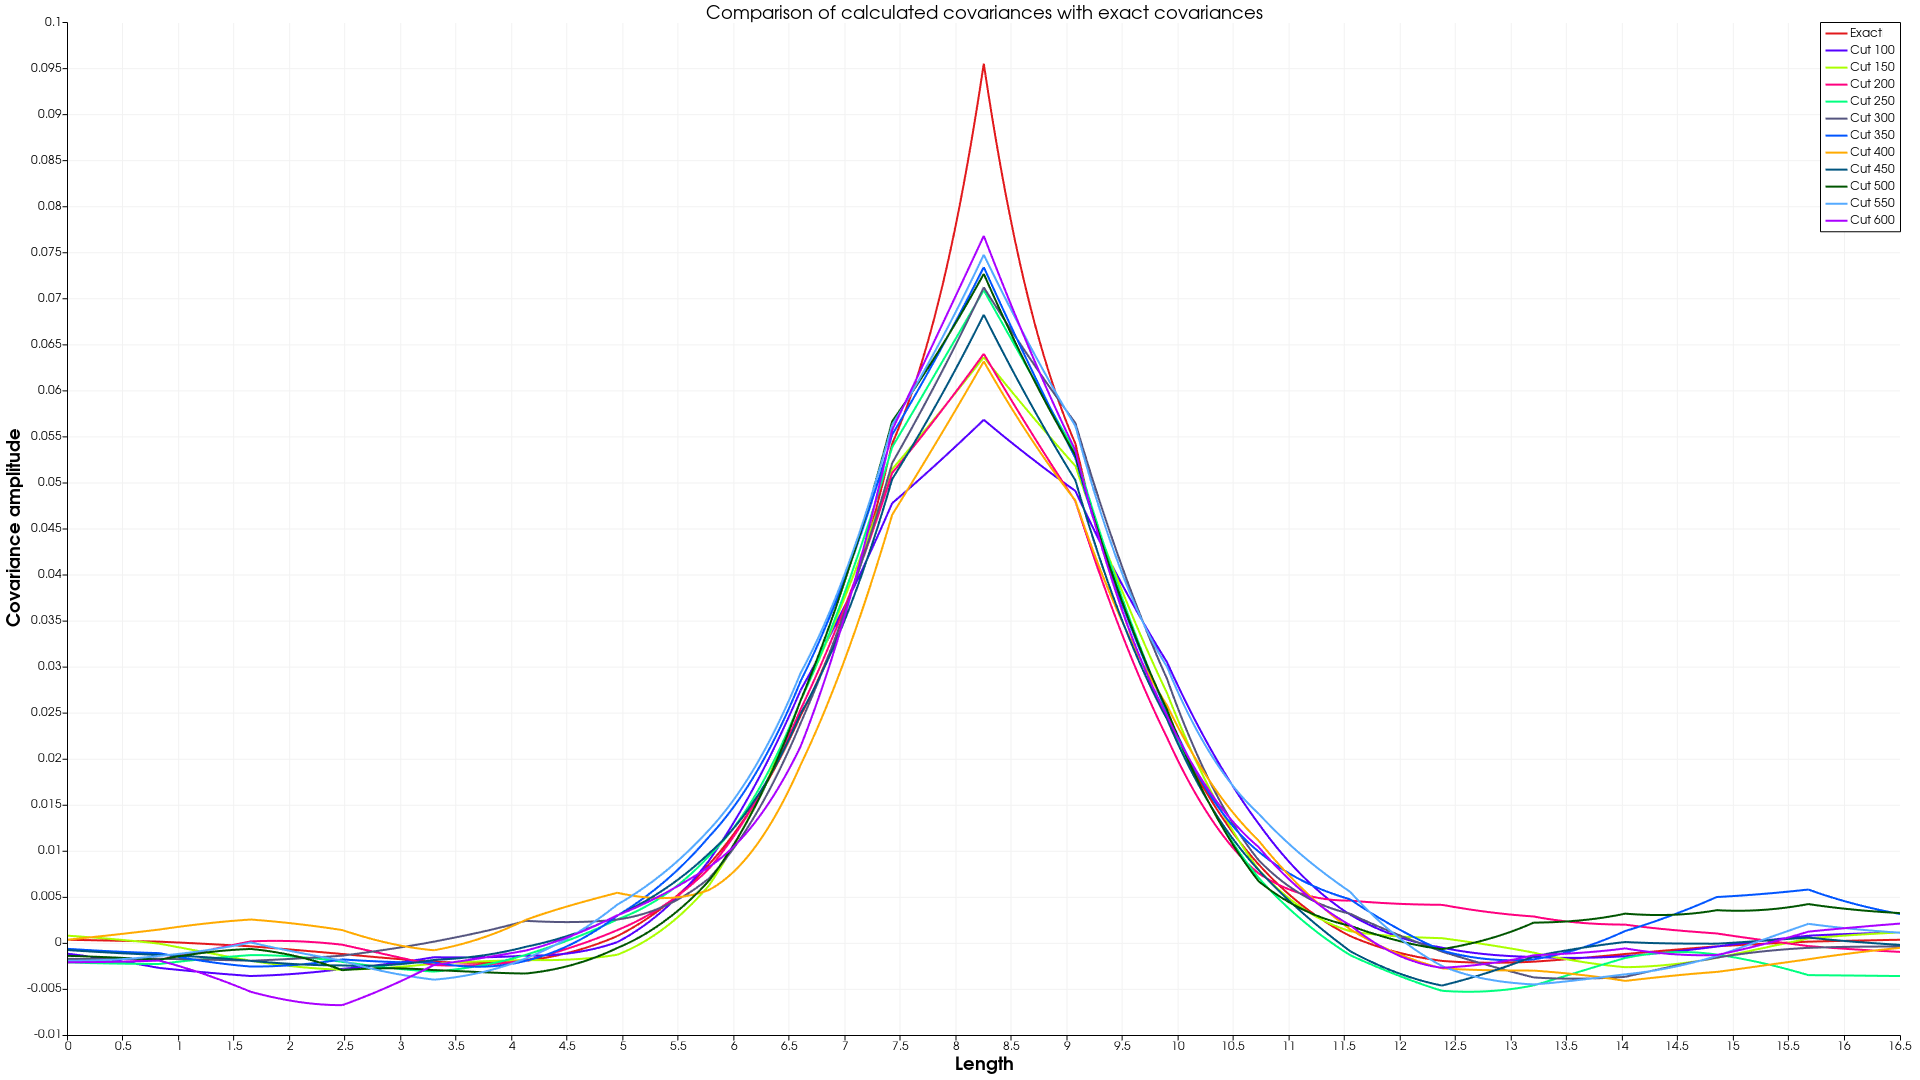
\includegraphics[width=0.4\linewidth]{comparison_covcut0_diag}}%
        \hfill       
        \subcaptionbox{$x$ направление\label{img:comparison_covcut0_x}} 
        {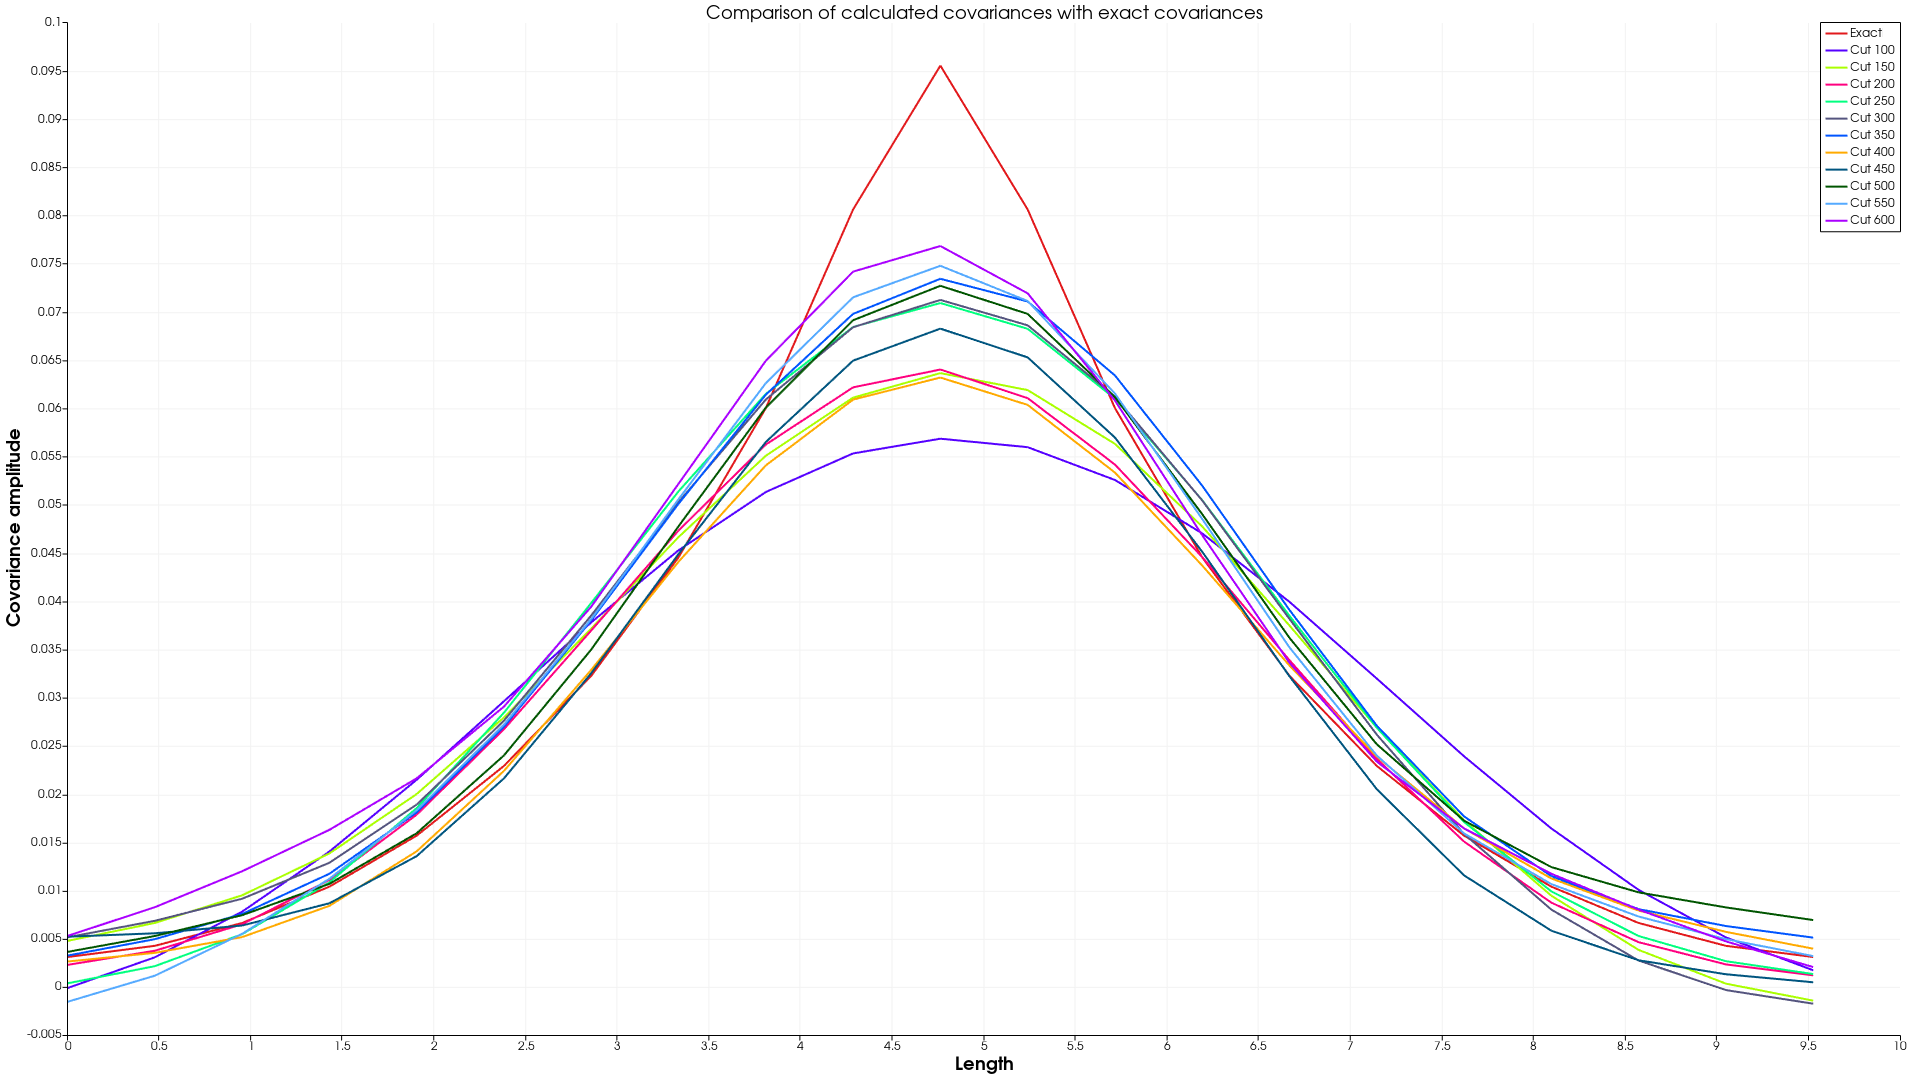
\includegraphics[width=0.4\linewidth]{comparison_covcut0_x}} \\
        \hfill
        \subcaptionbox[List-of-Figures entry]{$y$ направление\label{img:comparison_covcut0_y}} 
        {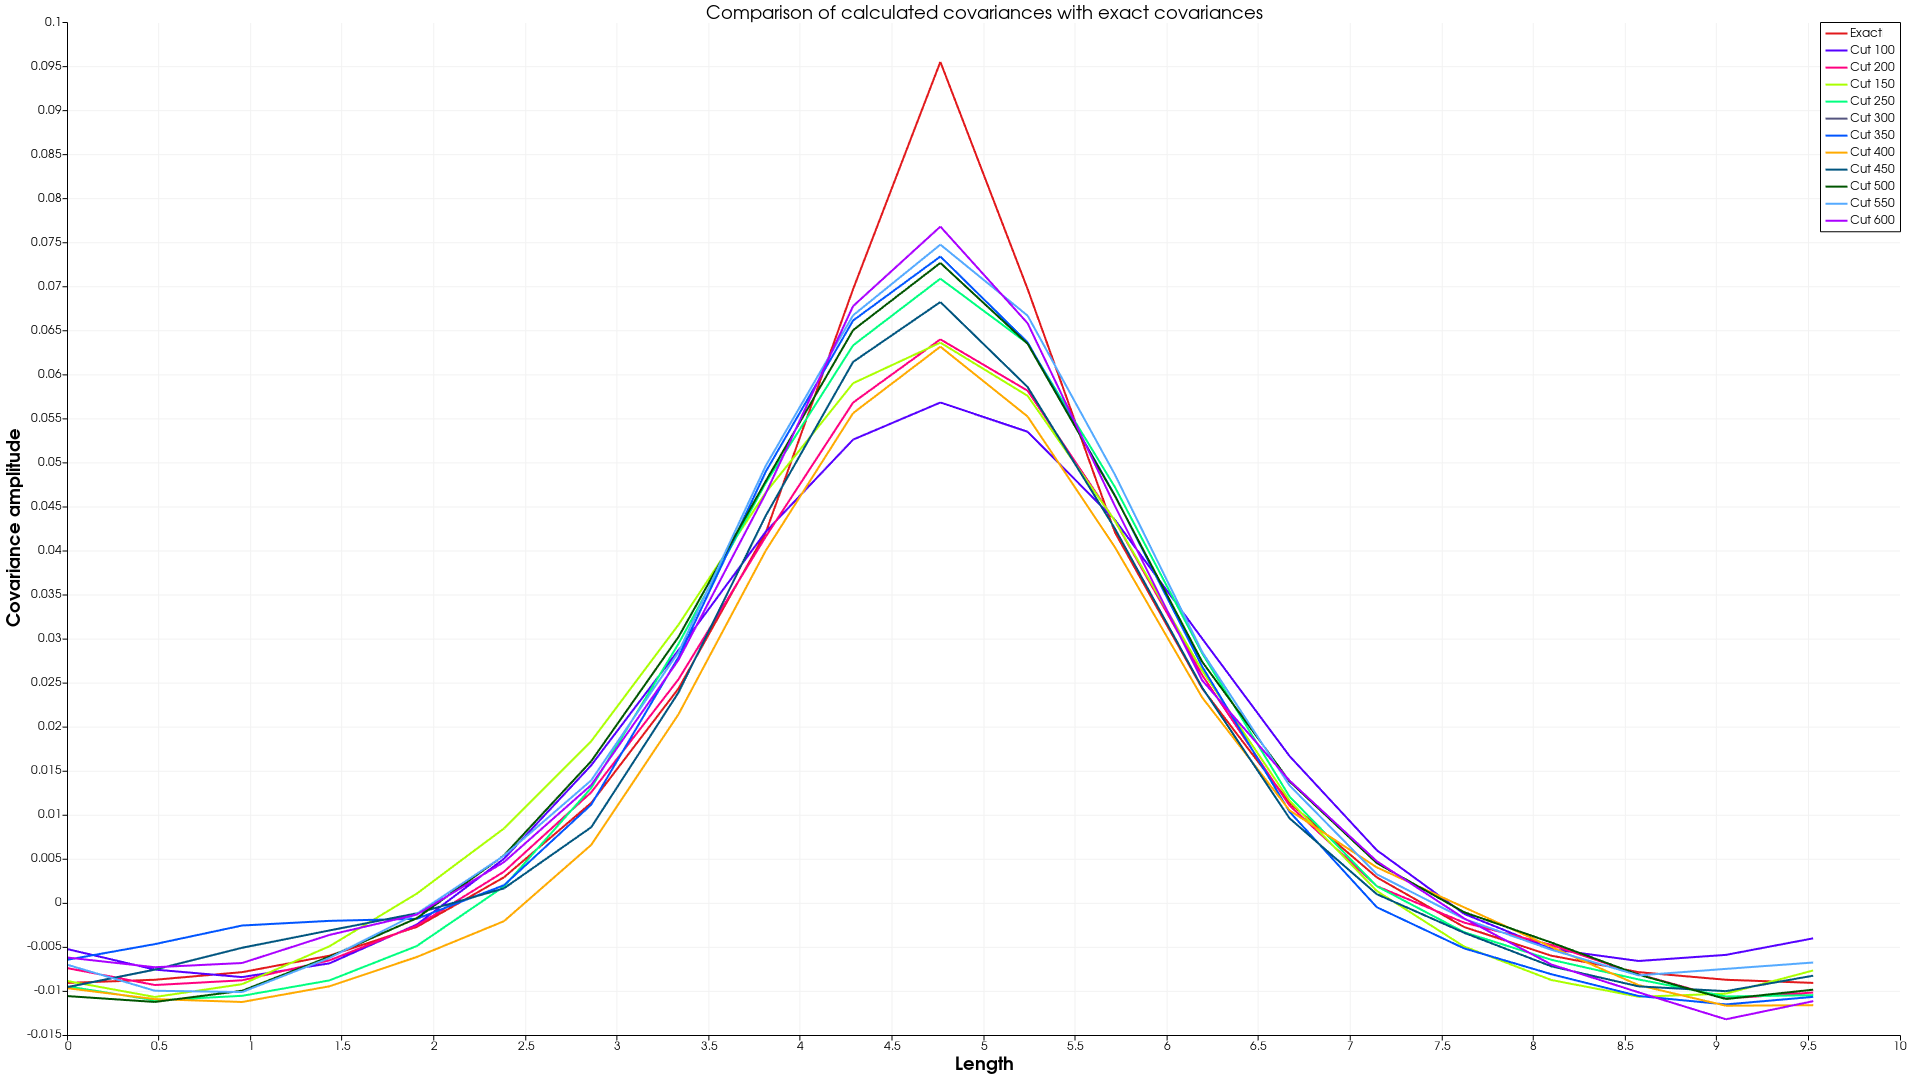
\includegraphics[width=0.4\linewidth]{comparison_covcut0_y}}%
        \hfill       
        \subcaptionbox{$z$ направление\label{img:comparison_covcut0_z}} 
        {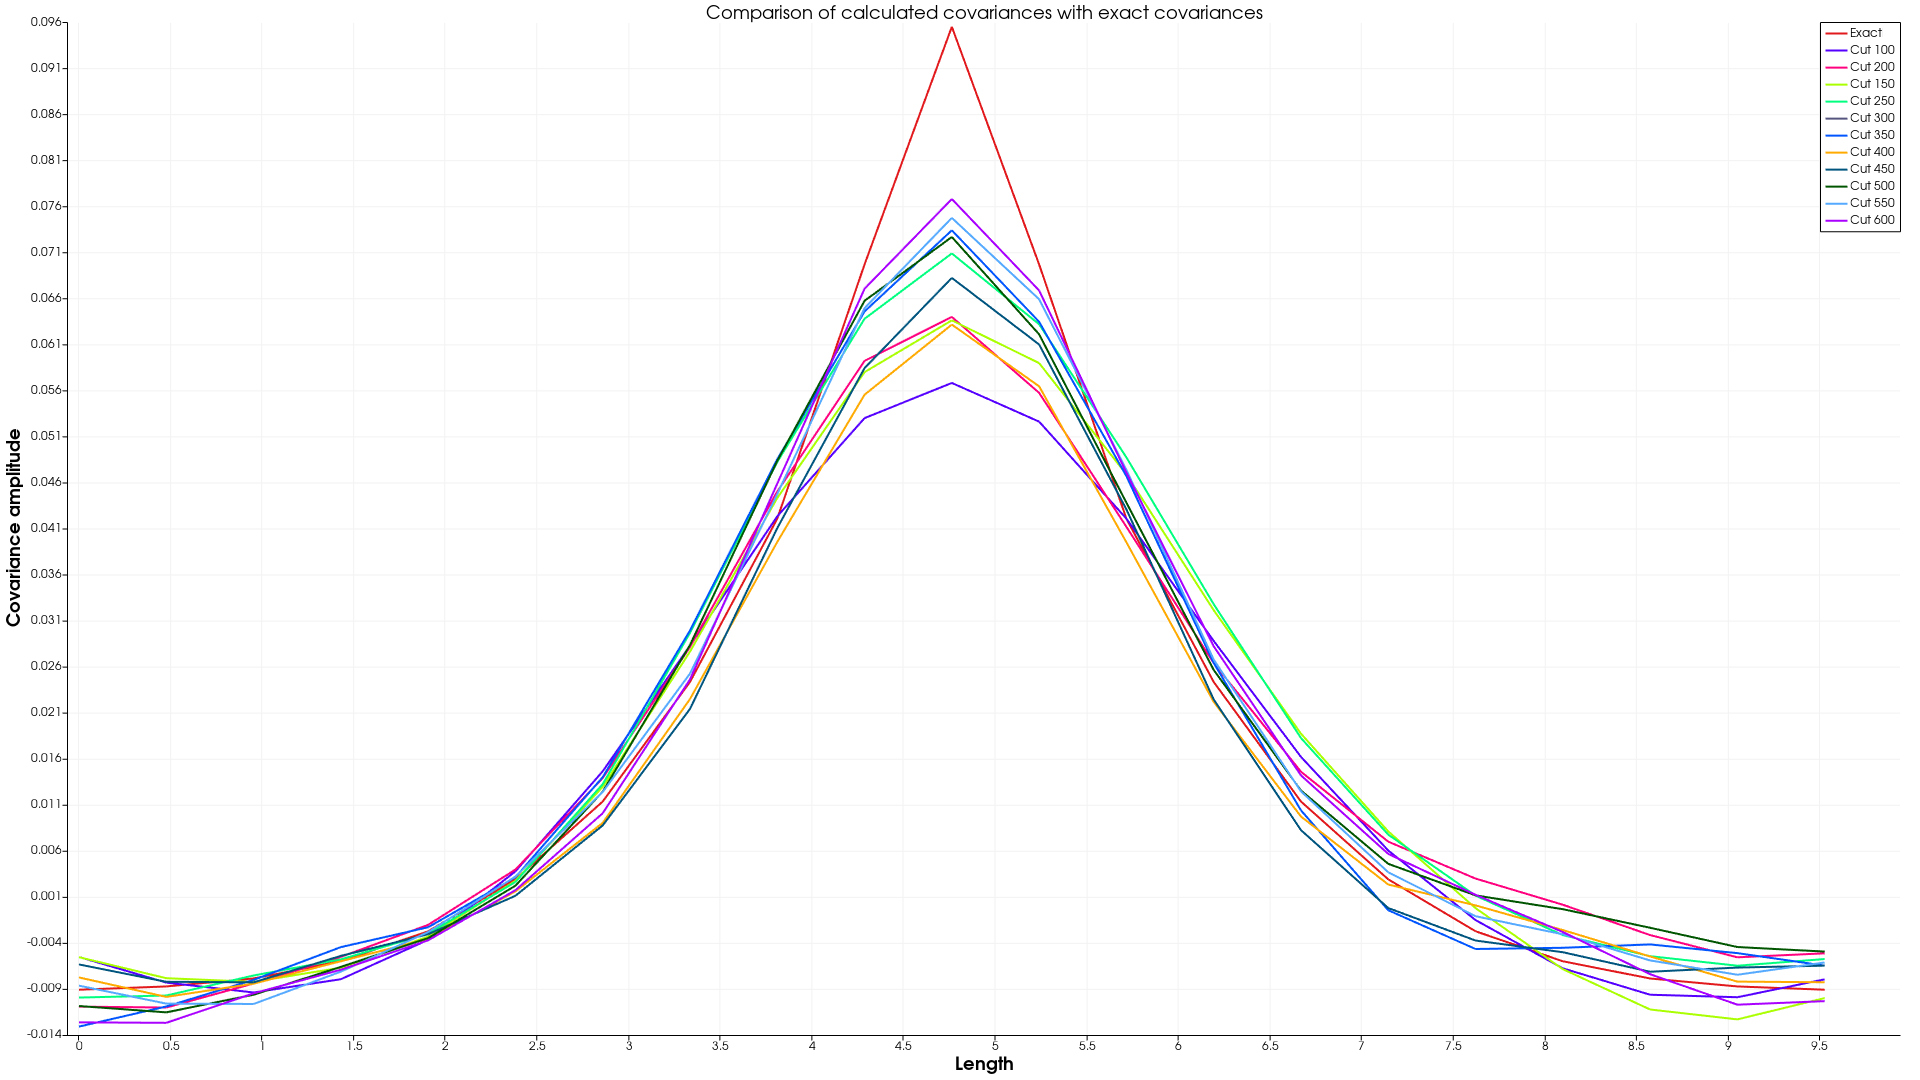
\includegraphics[width=0.4\linewidth]{comparison_covcut0_z}}
        \hfill
    }
    
    \onehalfspacing{Сравнение ковариацинной функции, допуск 0\%, для направлений а) вдоль диагонали, б) вдоль оси $x$, в) вдоль оси $y$, г) вдоль оси $z$}
    \caption{Сравнение ковариационной функции для допуска по амплитуде ковариаций в 0\% для различных направлений в рассматриваемой области}
    \label{img:covcut_0_comparison}  
\end{figure}
%
% Обрезание 1%
%
\begin{figure}[!h]
    \center{
        \hfill
        \subcaptionbox[List-of-Figures entry]{диагональ\label{img:comparison_covcut1_diag}} 
        {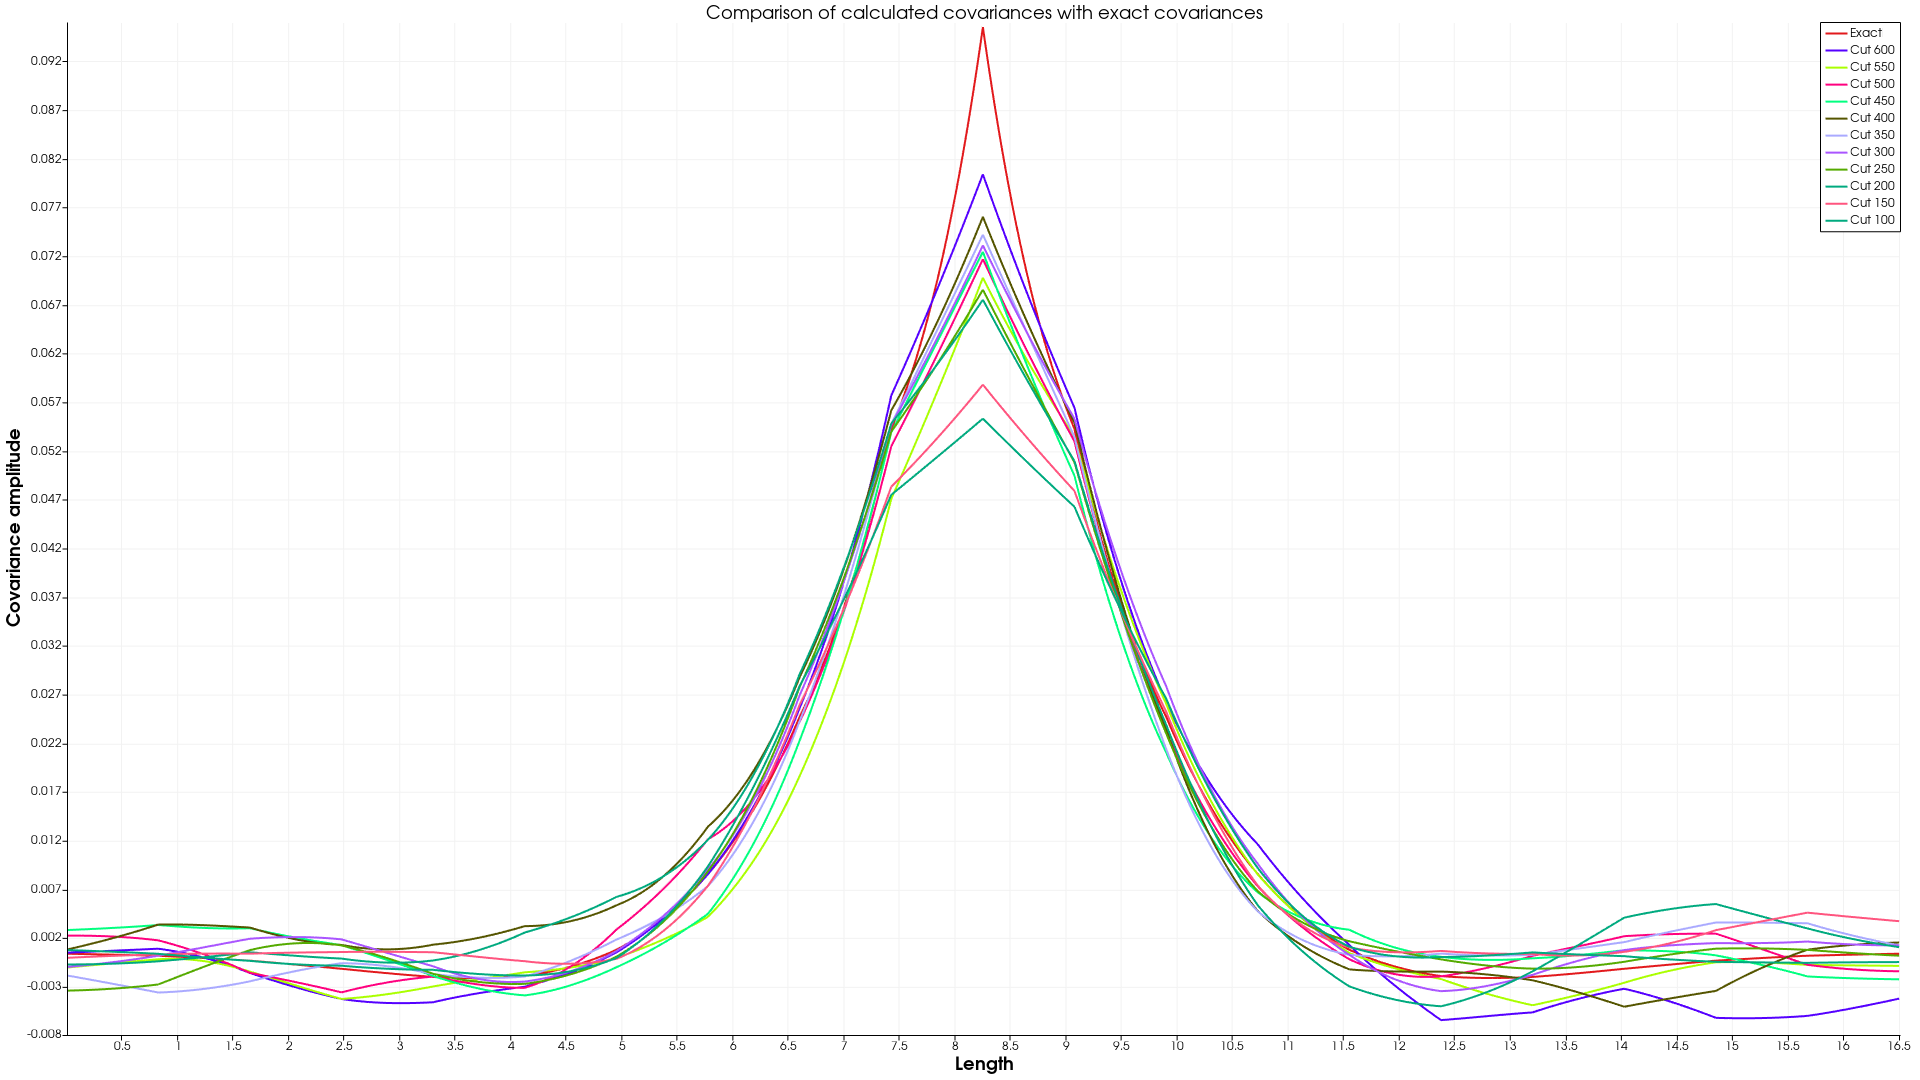
\includegraphics[width=0.4\linewidth]{comparison_covcut1_diag}}%
        \hfill       
        \subcaptionbox{$x$ направление\label{img:comparison_covcut1_x}} 
        {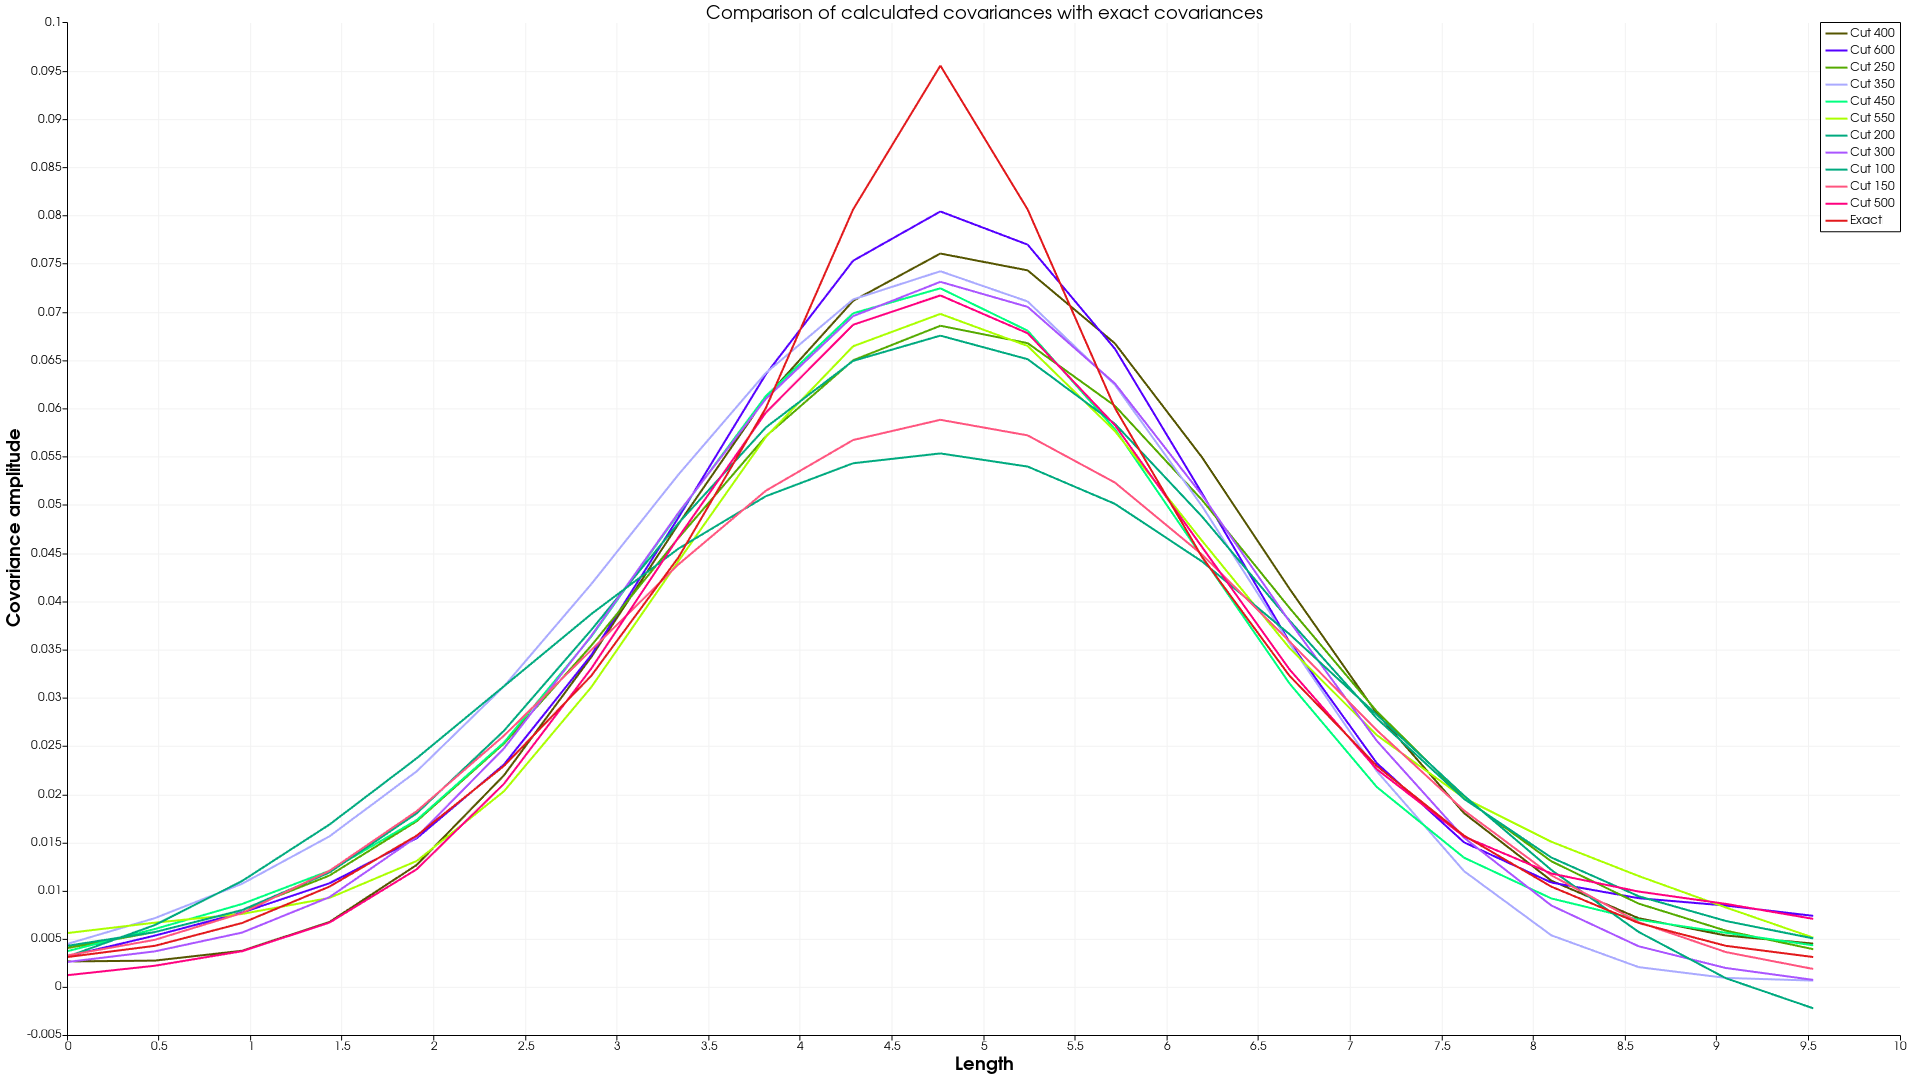
\includegraphics[width=0.4\linewidth]{comparison_covcut1_x}} \\
        \hfill
        \subcaptionbox[List-of-Figures entry]{$y$ направление\label{img:comparison_covcut1_y}} 
        {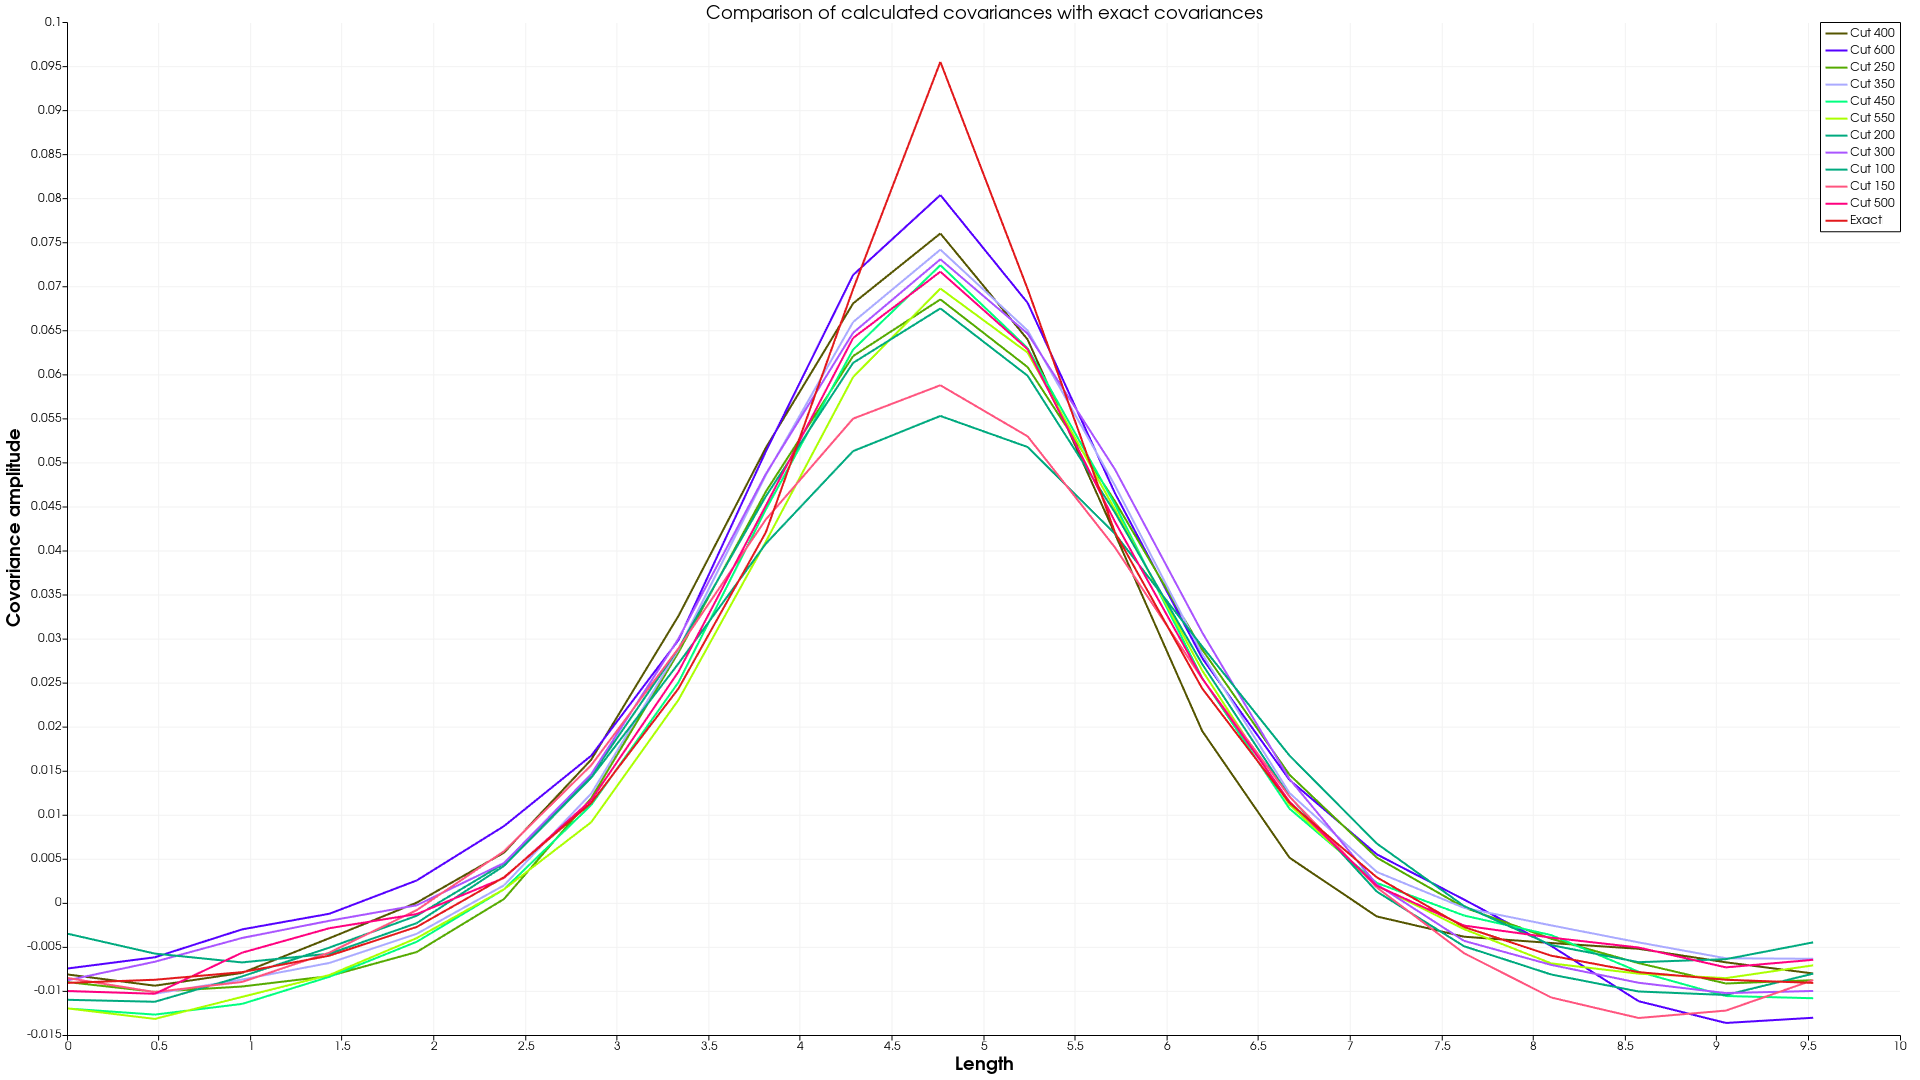
\includegraphics[width=0.4\linewidth]{comparison_covcut1_y}}%
        \hfill       
        \subcaptionbox{$z$ направление\label{img:comparison_covcut1_z}} 
        {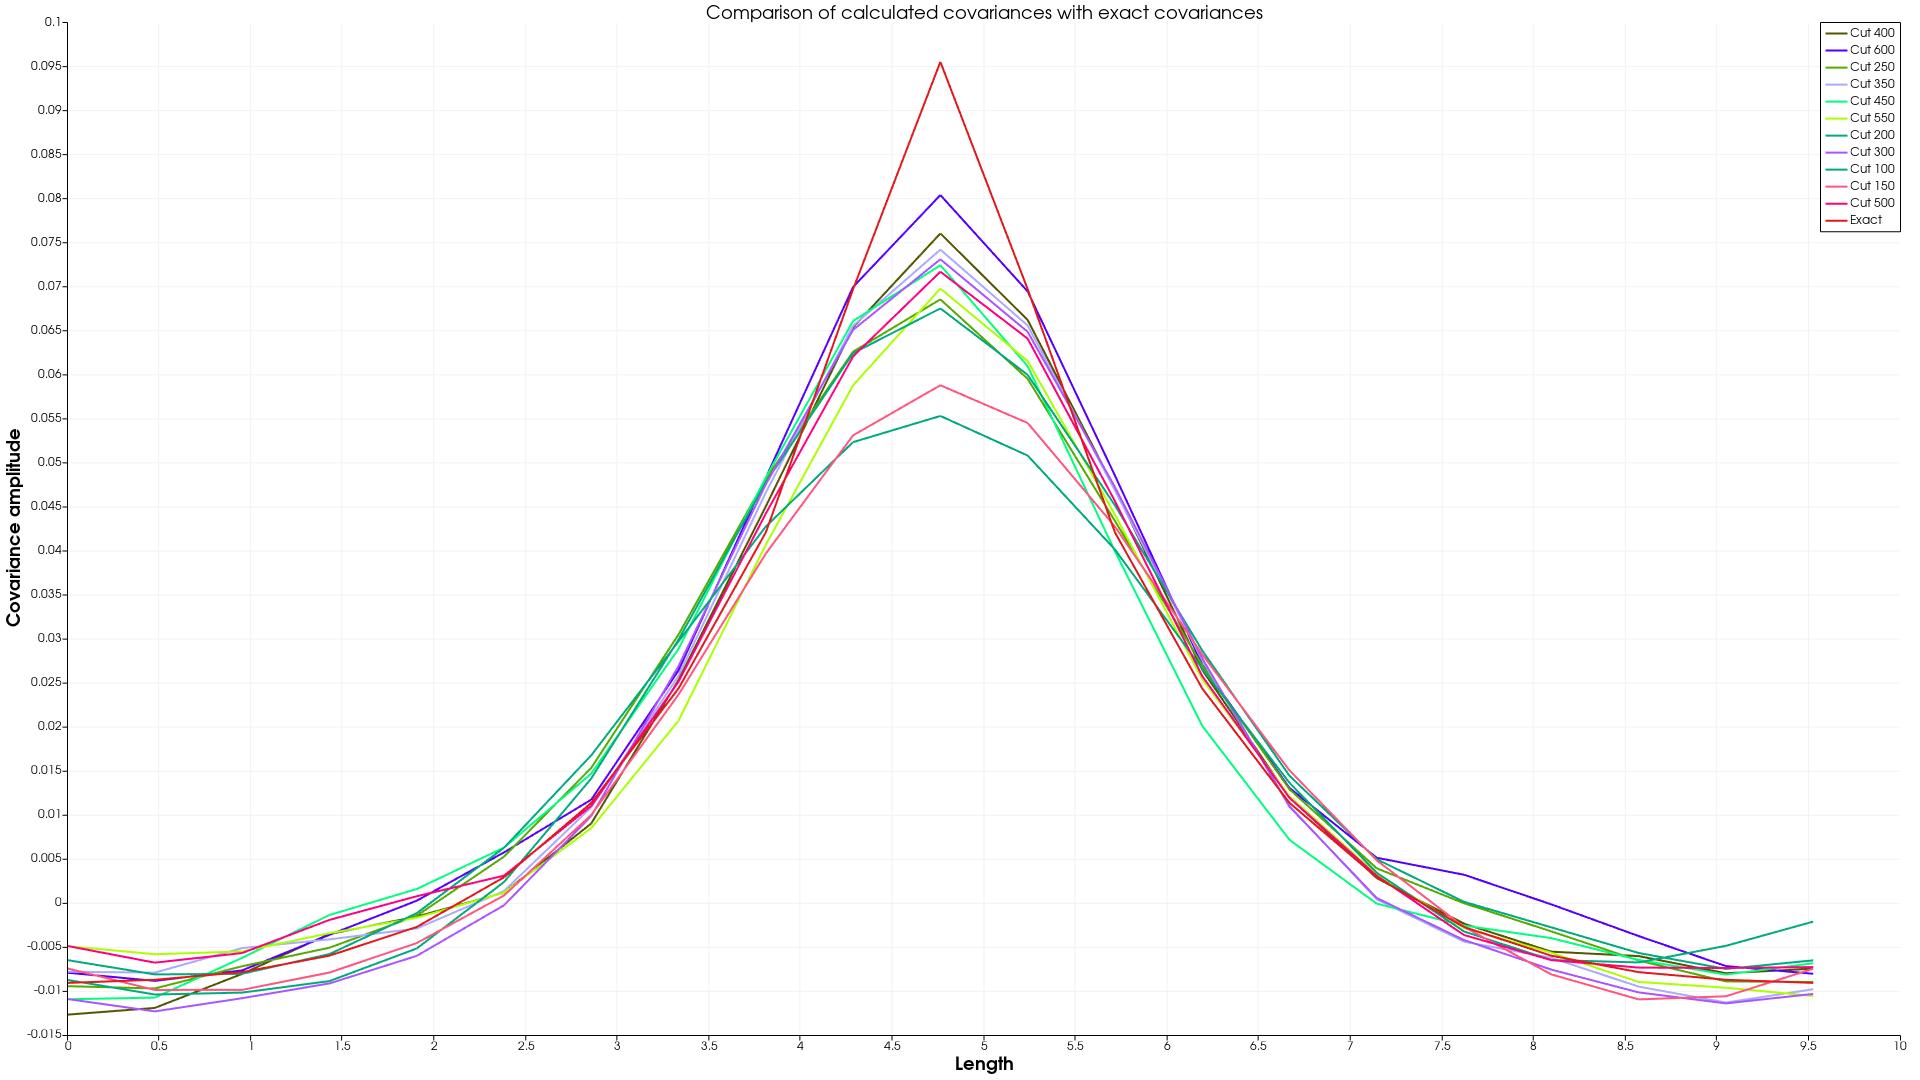
\includegraphics[width=0.4\linewidth]{comparison_covcut1_z}}
        \hfill
    }
    
    \onehalfspacing{Сравнение ковариацинной функции, допуск 1\%, для направлений а) вдоль диагонали, б) вдоль оси $x$, в) вдоль оси $y$, г) вдоль оси $z$}
    \caption{Сравнение ковариационной функции для допуска по амплитуде ковариаций в 1\% для различных направлений в рассматриваемой области}
    \label{img:covcut_1_comparison}  
\end{figure}
%
% Обрезание 2%
%
\begin{figure}[!h]
    \center{
        \hfill
        \subcaptionbox[List-of-Figures entry]{диагональ\label{img:comparison_covcut2_diag}} 
        {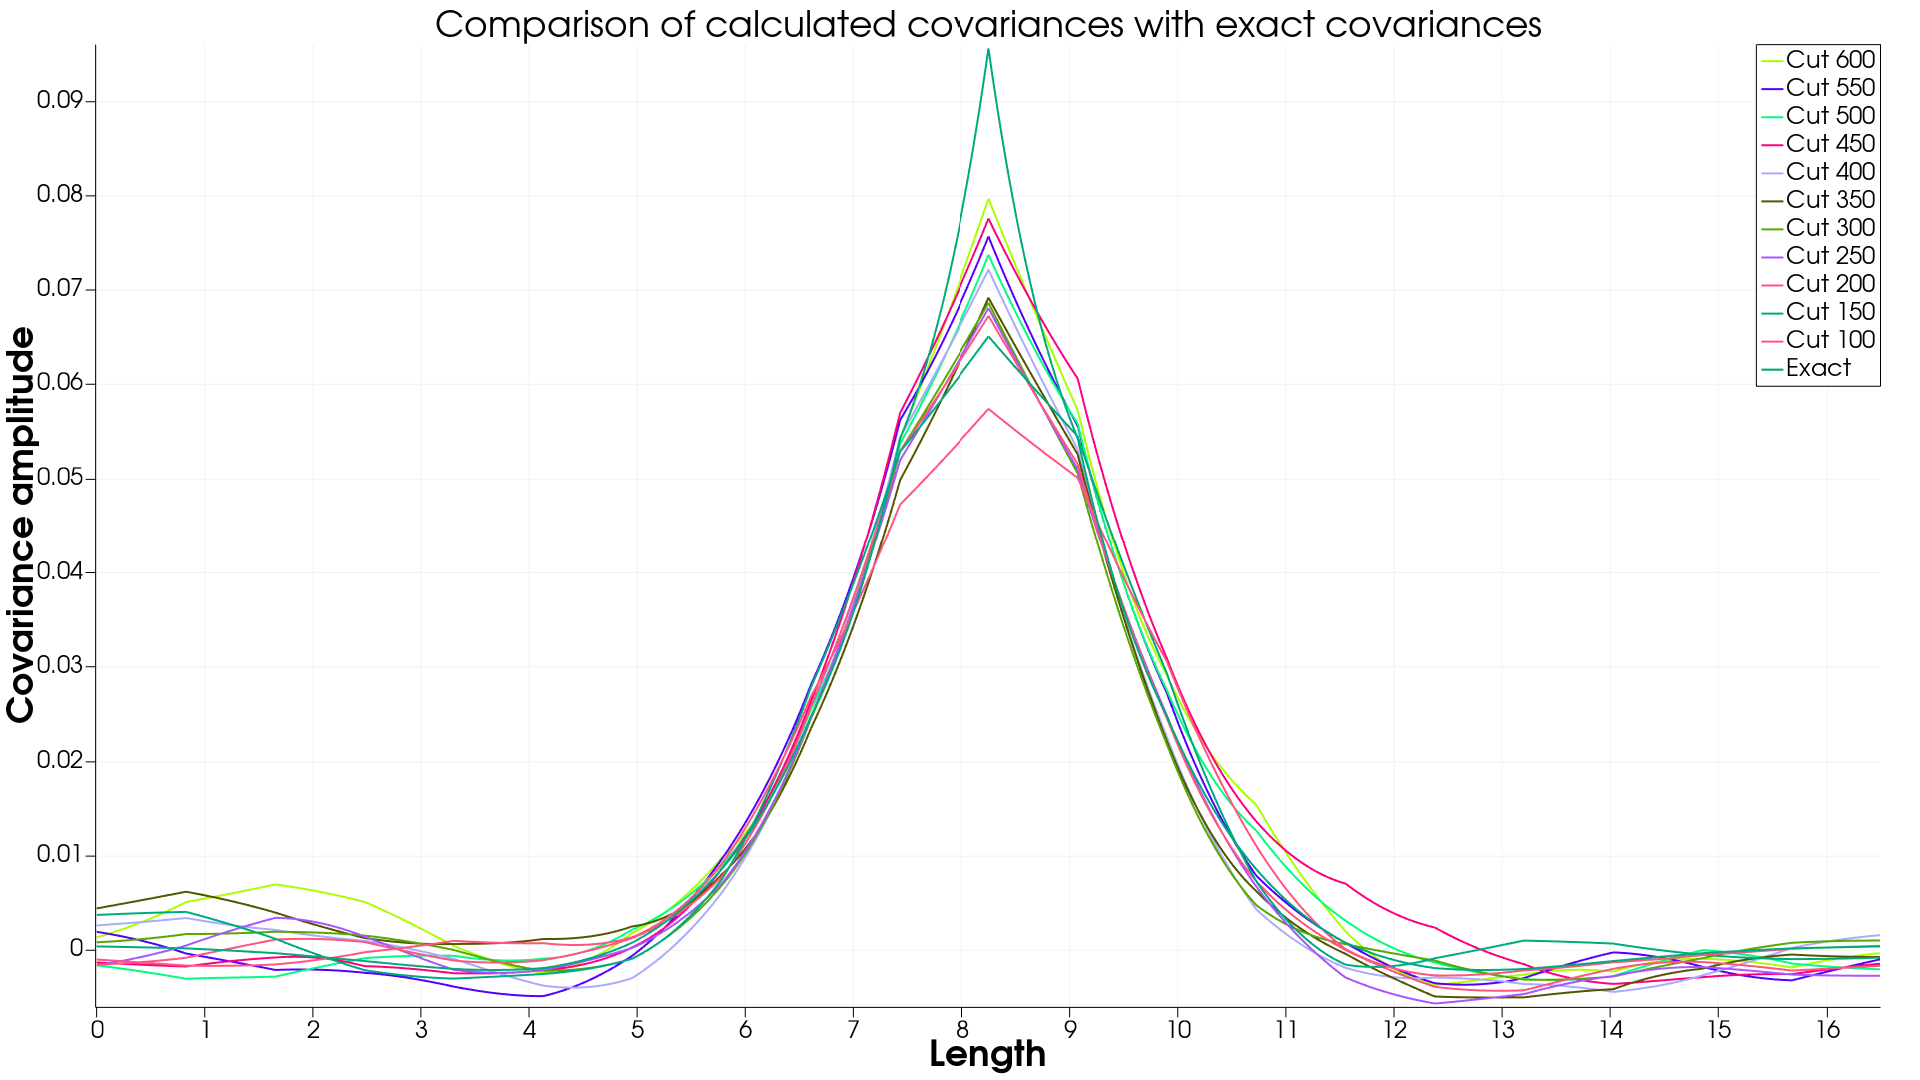
\includegraphics[width=0.4\linewidth]{comparison_covcut2_diag}}%
        \hfill       
        \subcaptionbox{$x$ направление\label{img:comparison_covcut1_x}} 
        {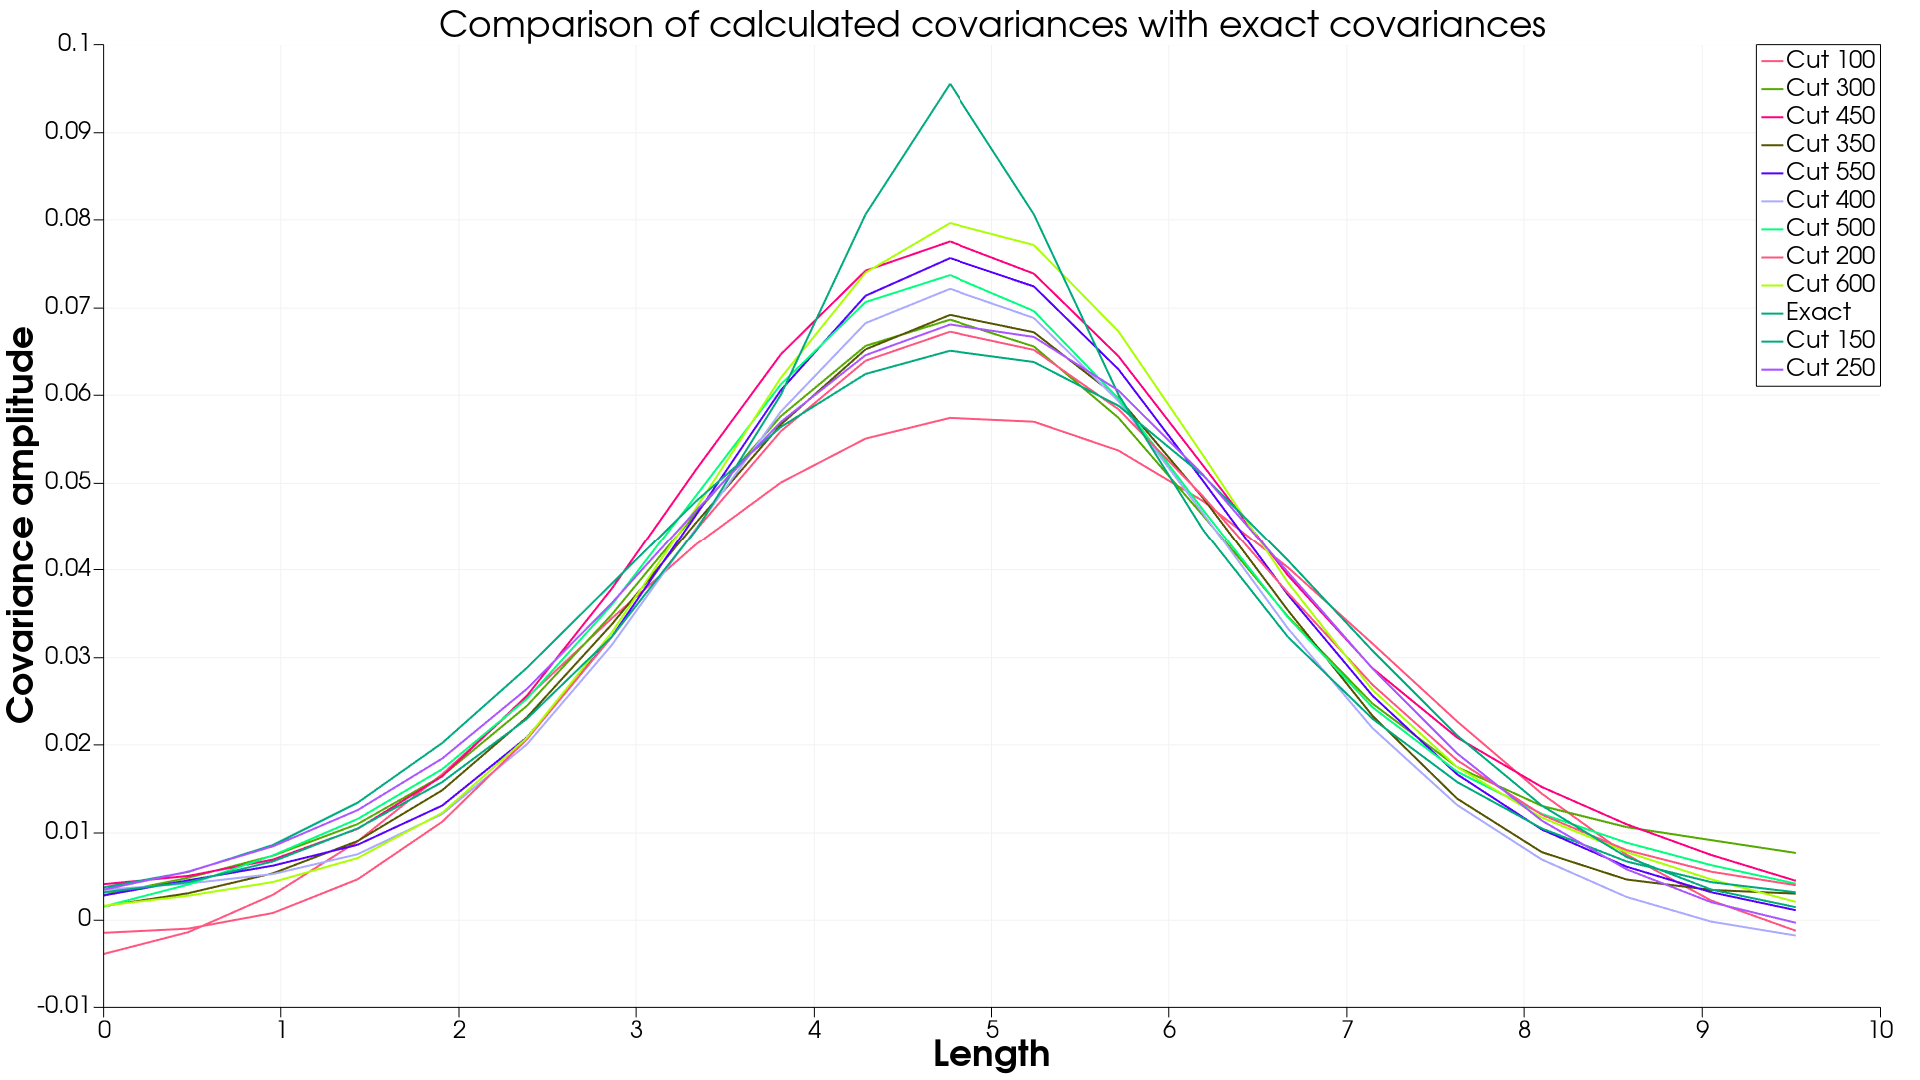
\includegraphics[width=0.4\linewidth]{comparison_covcut2_x}} \\
        \hfill
        \subcaptionbox[List-of-Figures entry]{$y$ направление\label{img:comparison_covcut2_y}} 
        {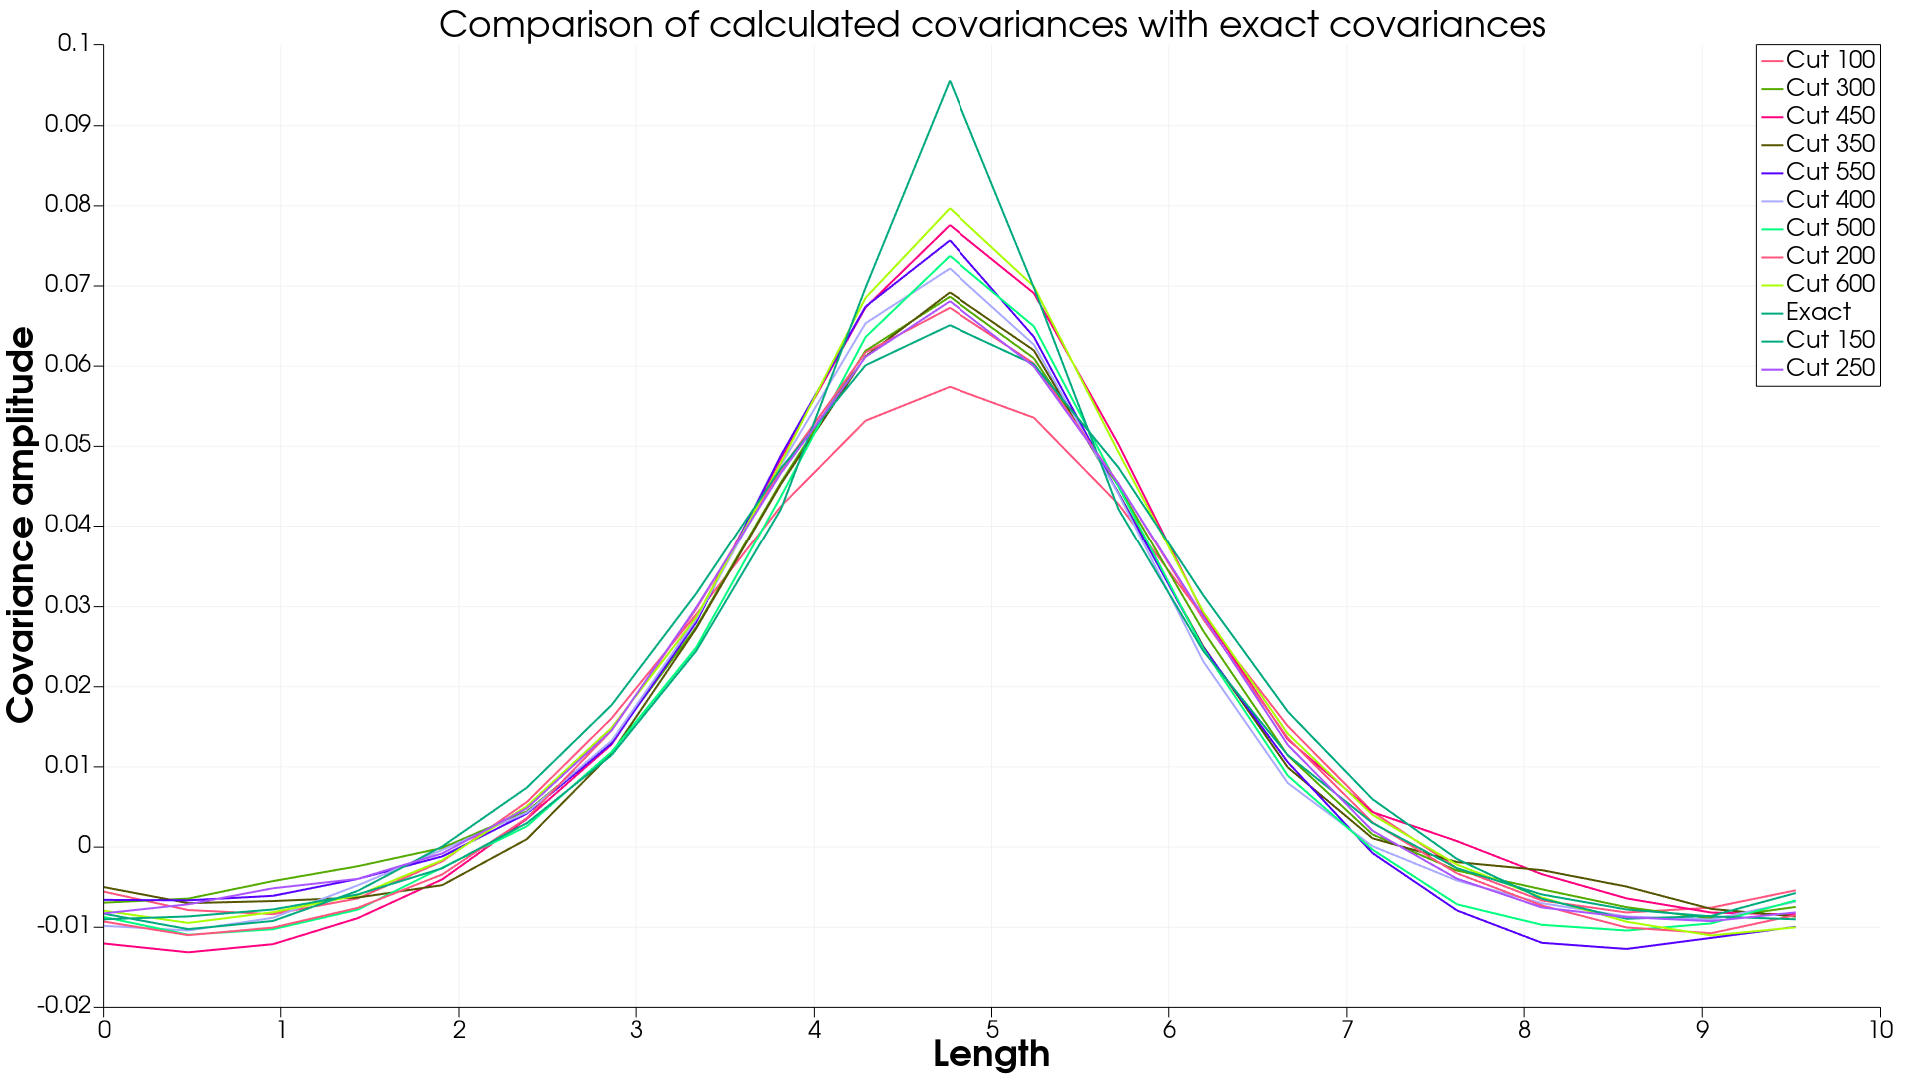
\includegraphics[width=0.4\linewidth]{comparison_covcut2_y}}%
        \hfill       
        \subcaptionbox{$z$ направление\label{img:comparison_covcut2_z}} 
        {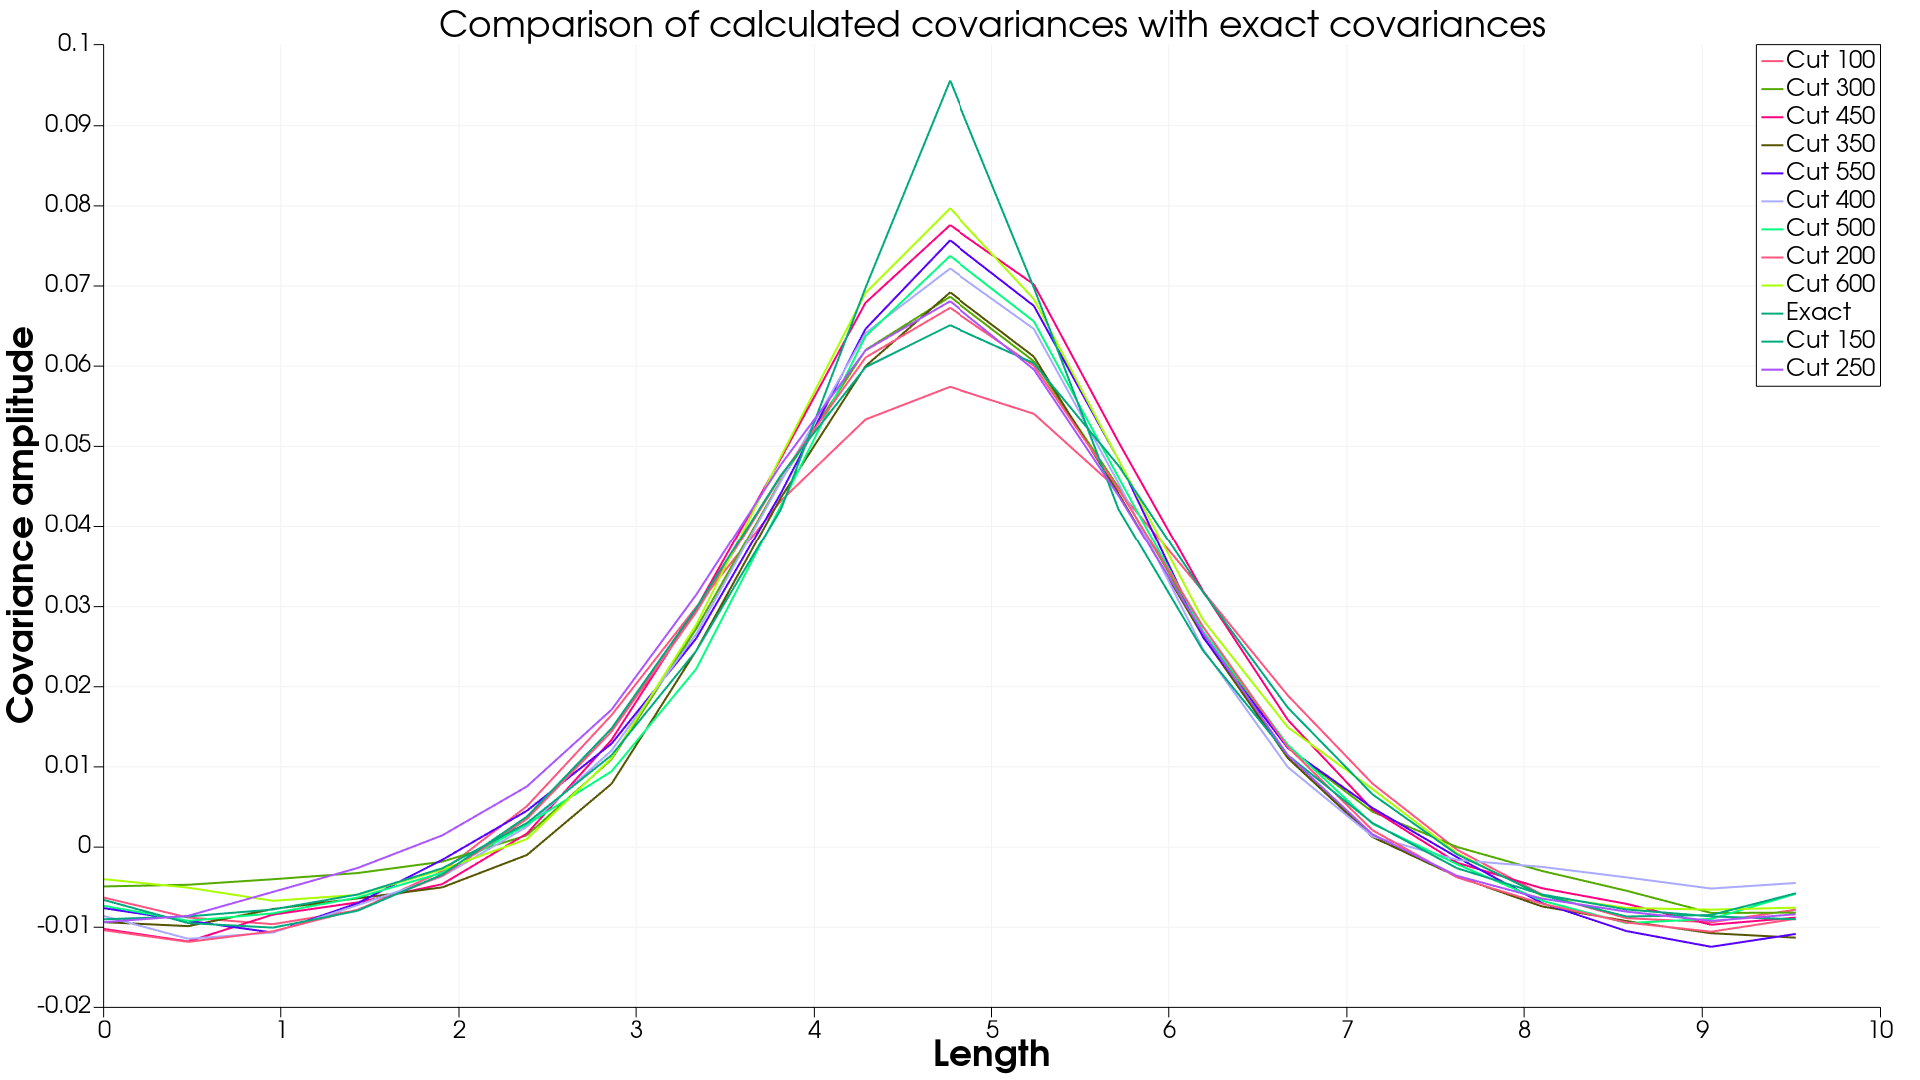
\includegraphics[width=0.4\linewidth]{comparison_covcut2_z}}
        \hfill
    }
    
    \onehalfspacing{Сравнение ковариацинной функции, допуск 2\%, для направлений а) вдоль диагонали, б) вдоль оси $x$, в) вдоль оси $y$, г) вдоль оси $z$}
    \caption{Сравнение ковариационной функции для допуска по амплитуде ковариаций в 2\% для различных направлений в рассматриваемой области}
    \label{img:covcut_2_comparison}  
\end{figure}
%
% Обрезание 3%
%
\begin{figure}[!h]
    \center{
        \hfill
        \subcaptionbox[List-of-Figures entry]{диагональ\label{img:comparison_covcut3_diag}} 
        {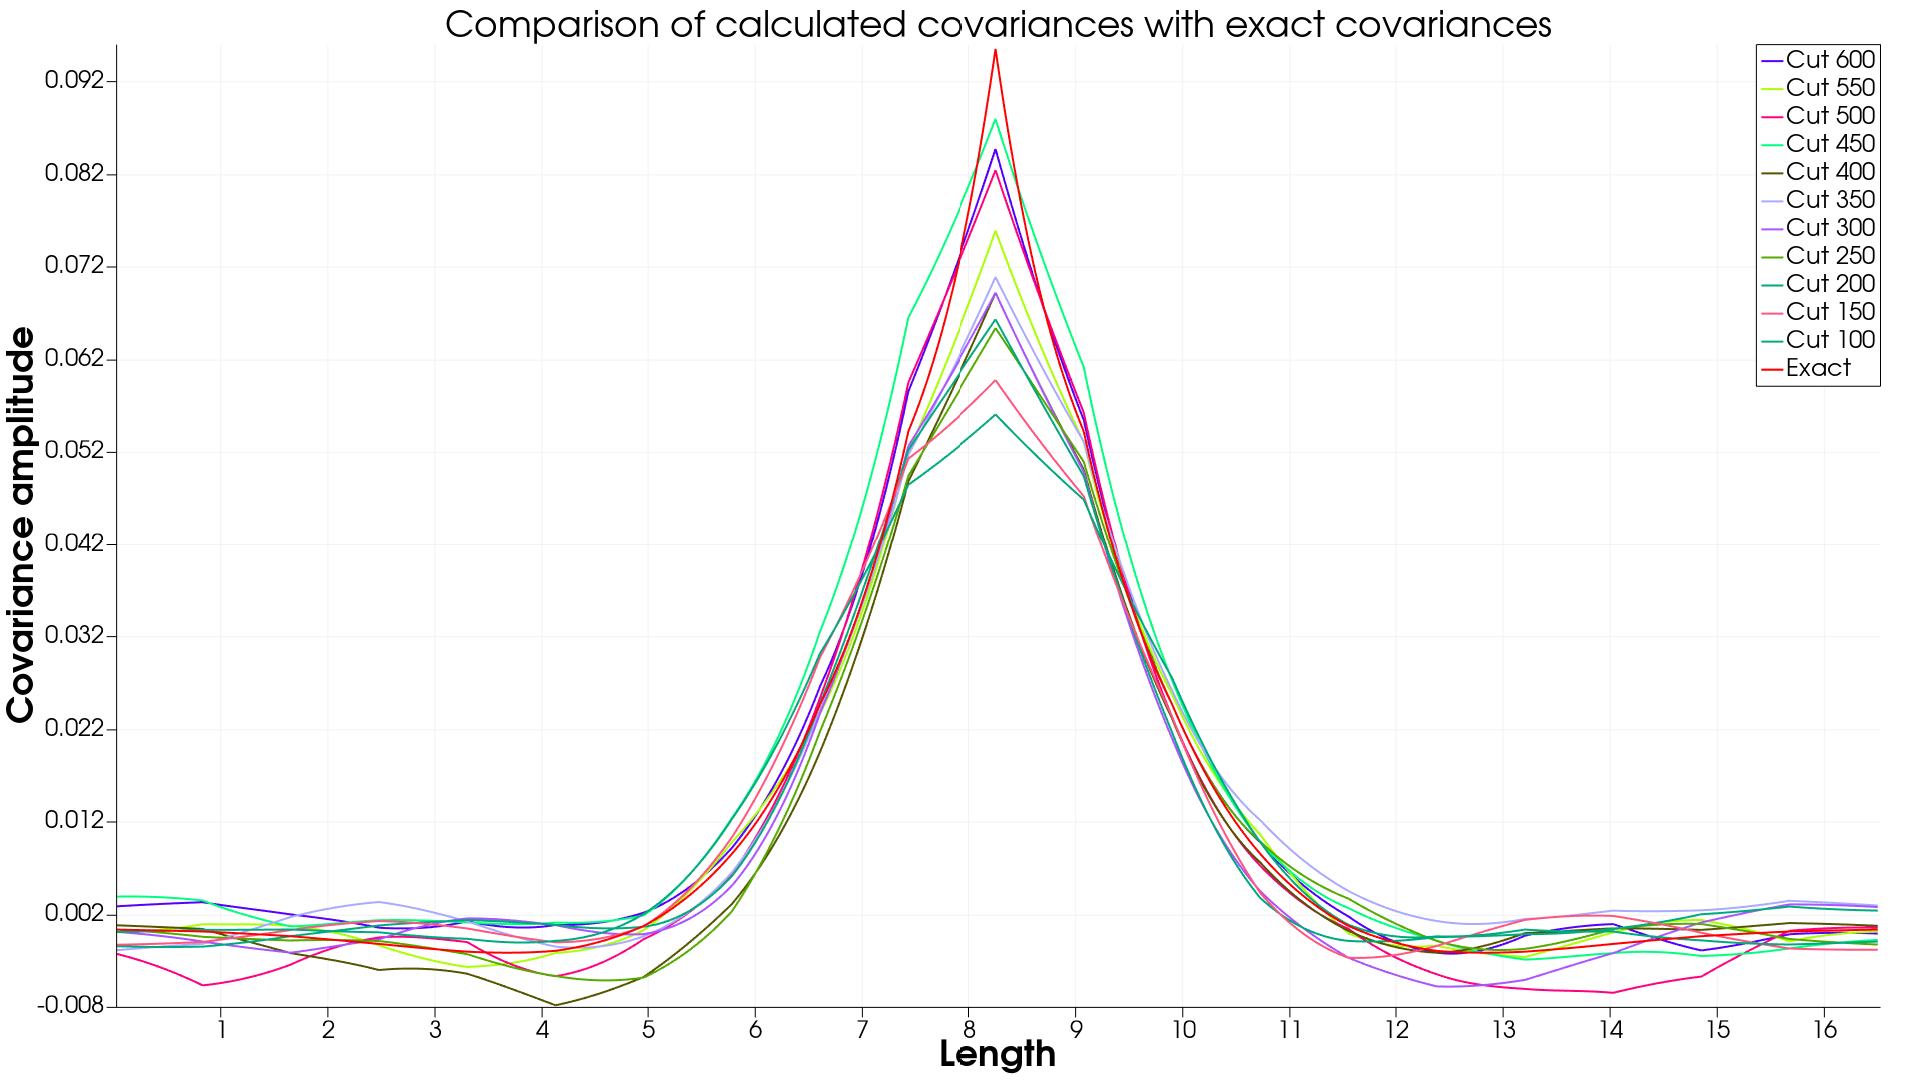
\includegraphics[width=0.4\linewidth]{comparison_covcut3_diag}}%
        \hfill       
        \subcaptionbox{$x$ направление\label{img:comparison_covcut3_x}} 
        {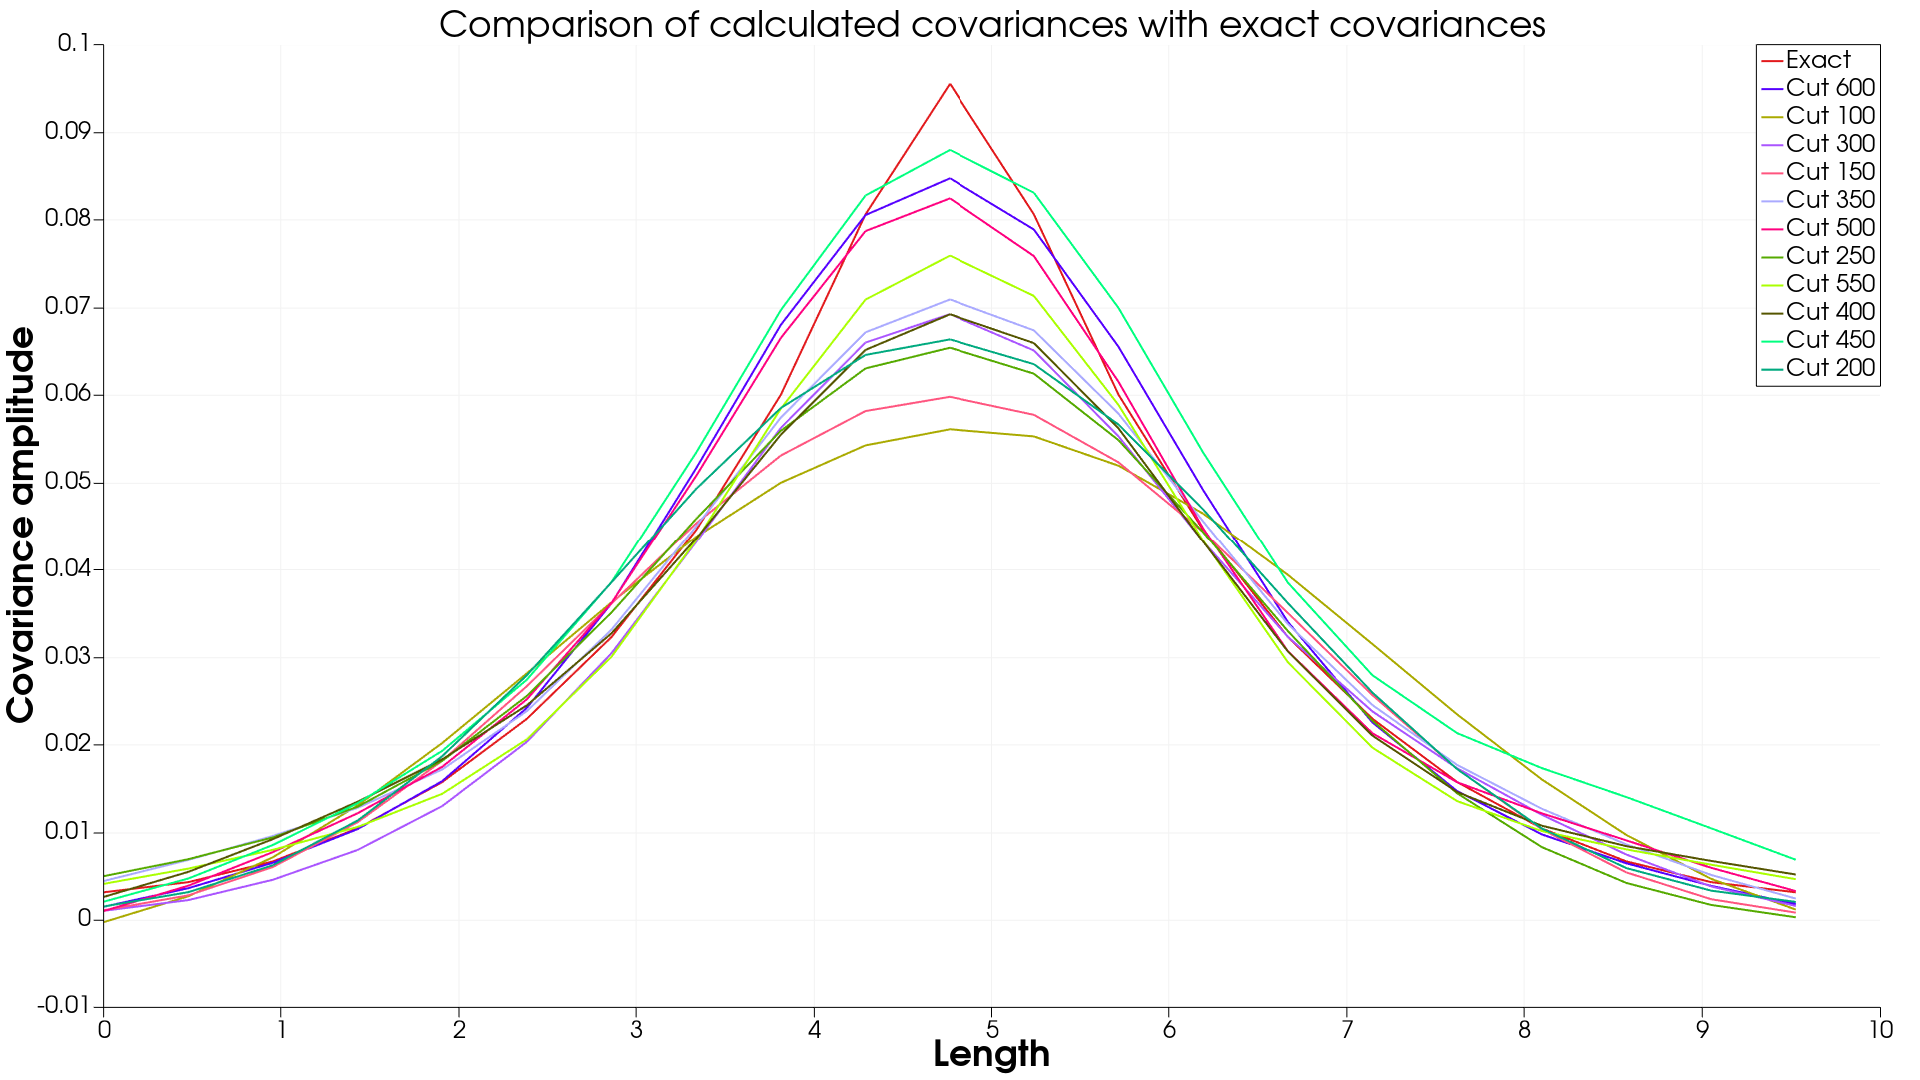
\includegraphics[width=0.4\linewidth]{comparison_covcut3_x}} \\
        \hfill
        \subcaptionbox[List-of-Figures entry]{$y$ направление\label{img:comparison_covcut3_y}} 
        {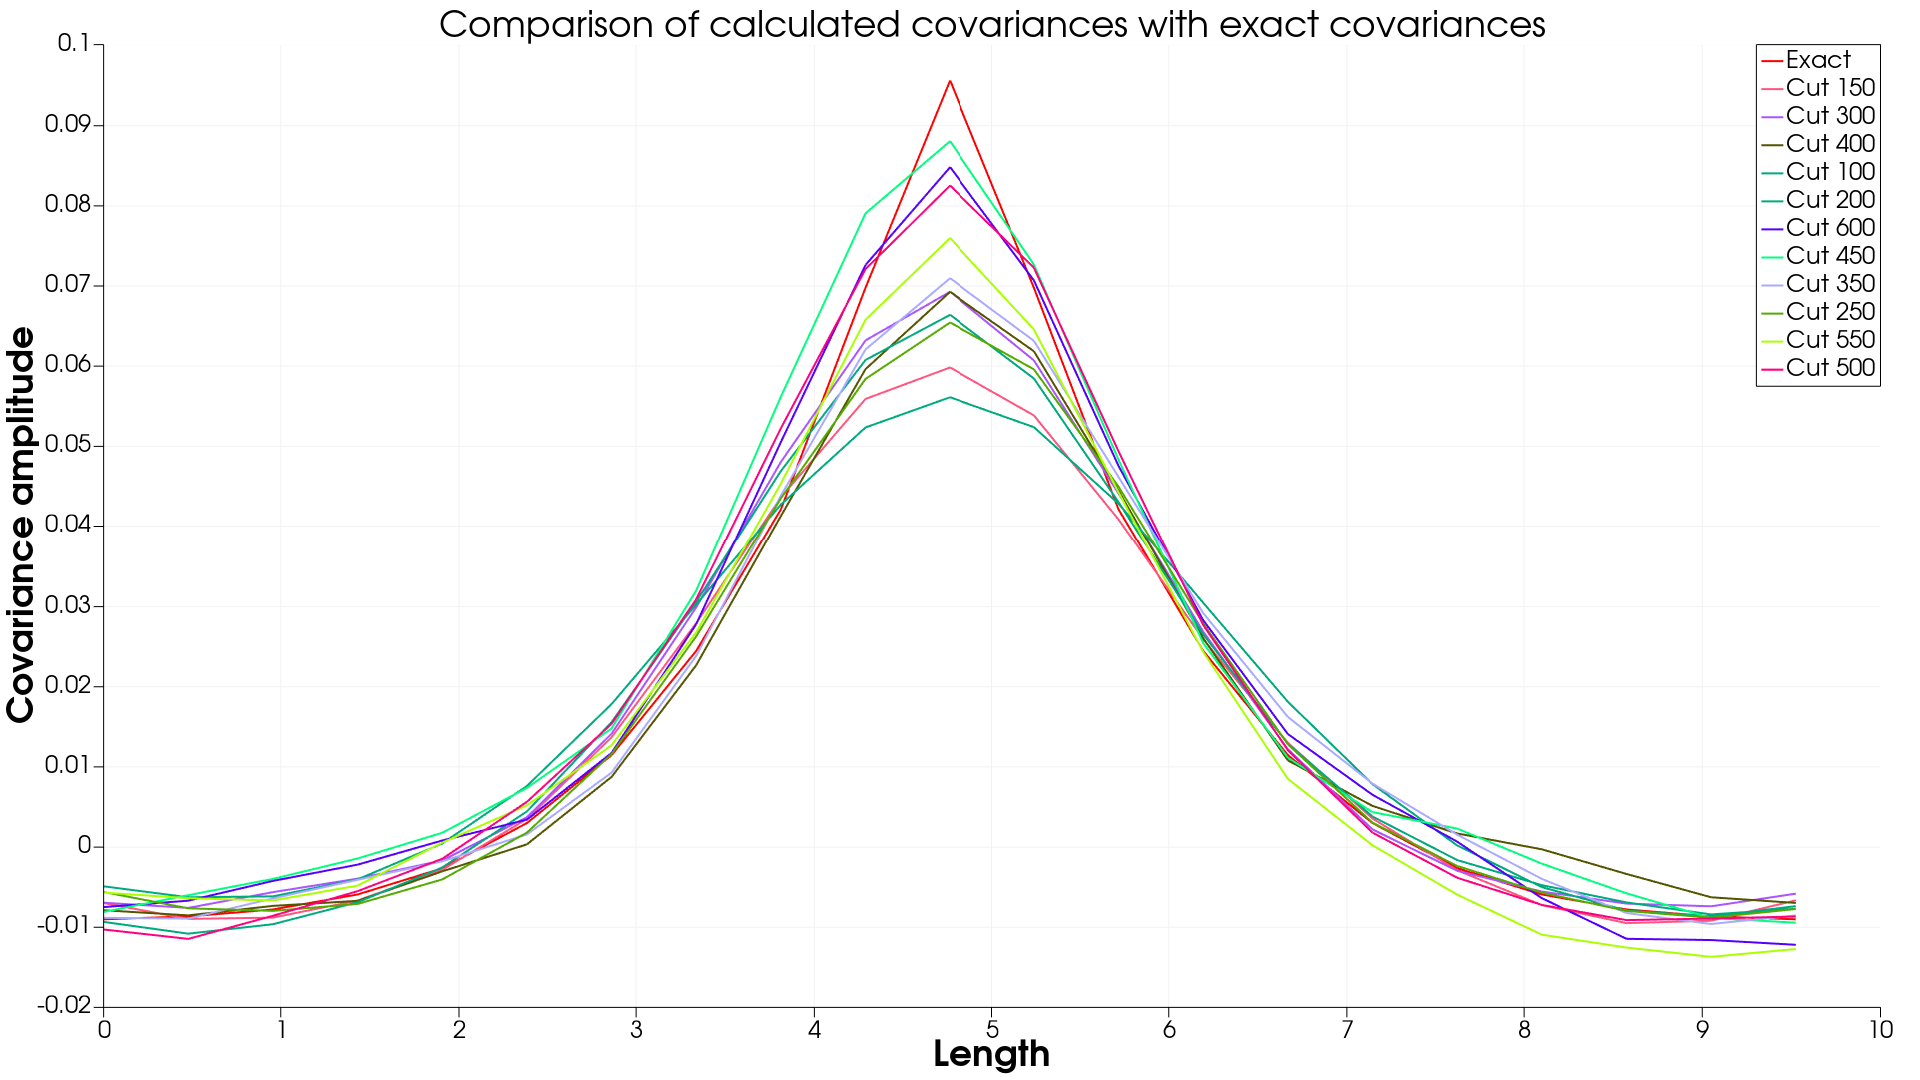
\includegraphics[width=0.4\linewidth]{comparison_covcut3_y}}%
        \hfill       
        \subcaptionbox{$z$ направление\label{img:comparison_covcut3_z}} 
        {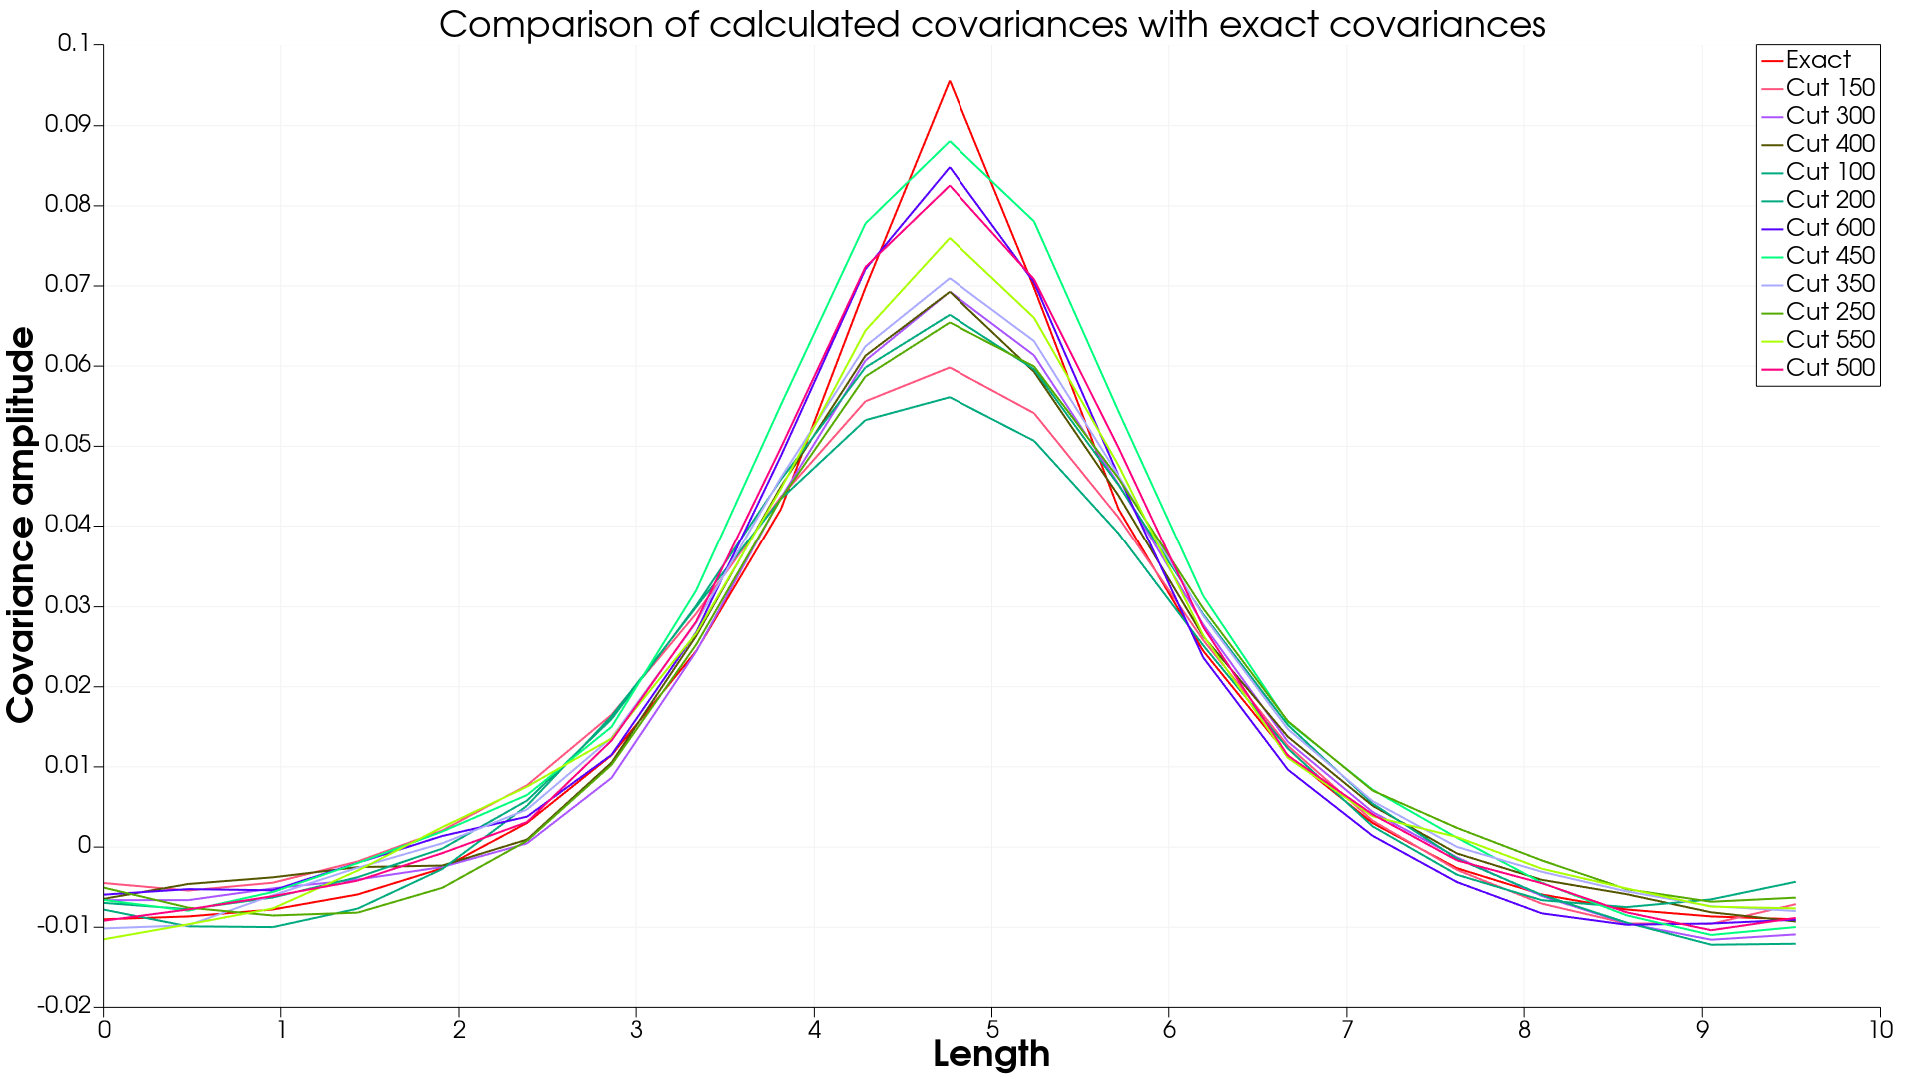
\includegraphics[width=0.4\linewidth]{comparison_covcut3_z}}
        \hfill
    }
    
    \onehalfspacing{Сравнение ковариацинной функции, допуск 3\%, для направлений а) вдоль диагонали, б) вдоль оси $x$, в) вдоль оси $y$, г) вдоль оси $z$}
    \caption{Сравнение ковариационной функции для допуска по амплитуде ковариаций в 3\% для различных направлений в рассматриваемой области}
    \label{img:covcut_3_comparison}  
\end{figure}
%
% Обрезание 4%
%
\begin{figure}[!h]
    \center{
        \hfill
        \subcaptionbox[List-of-Figures entry]{диагональ\label{img:comparison_covcut4_diag}} 
        {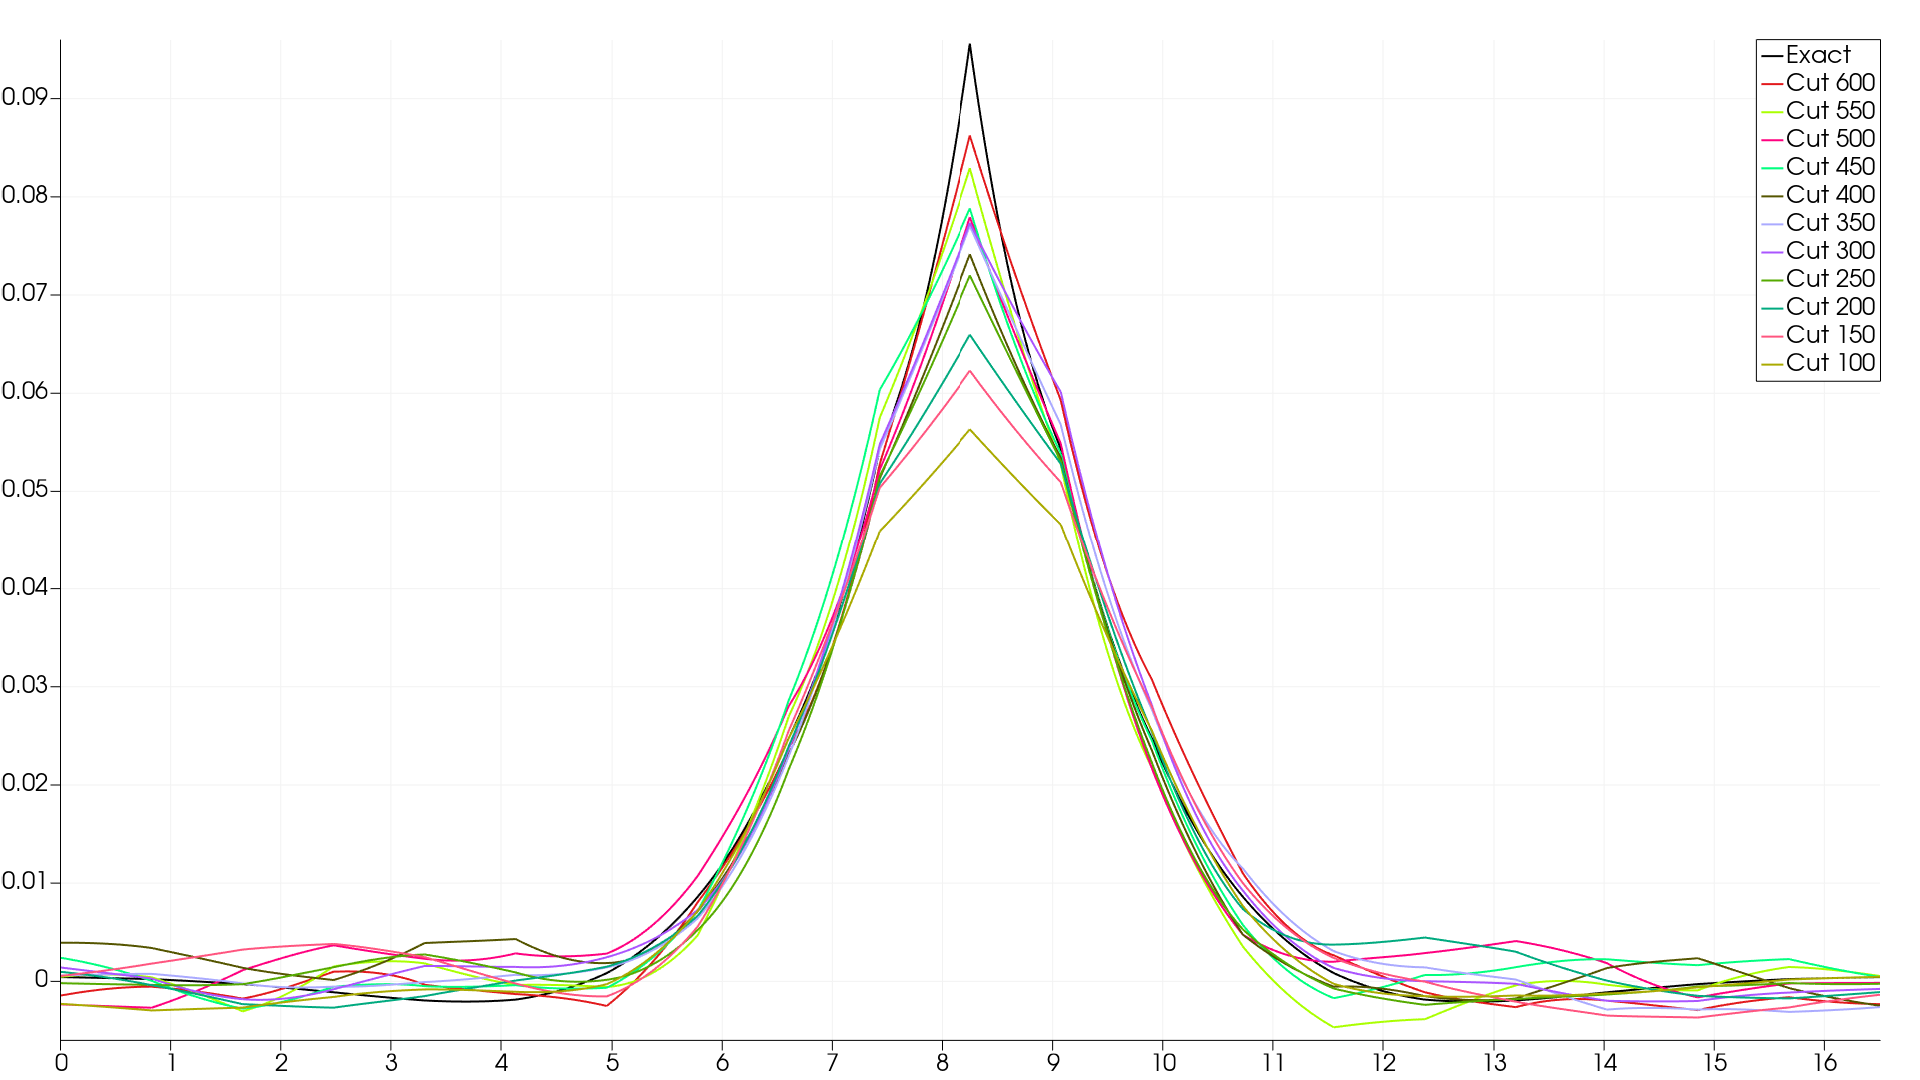
\includegraphics[width=0.4\linewidth]{comparison_covcut4_diag}}%
        \hfill       
        \subcaptionbox{$x$ направление\label{img:comparison_covcut4_y}} 
        {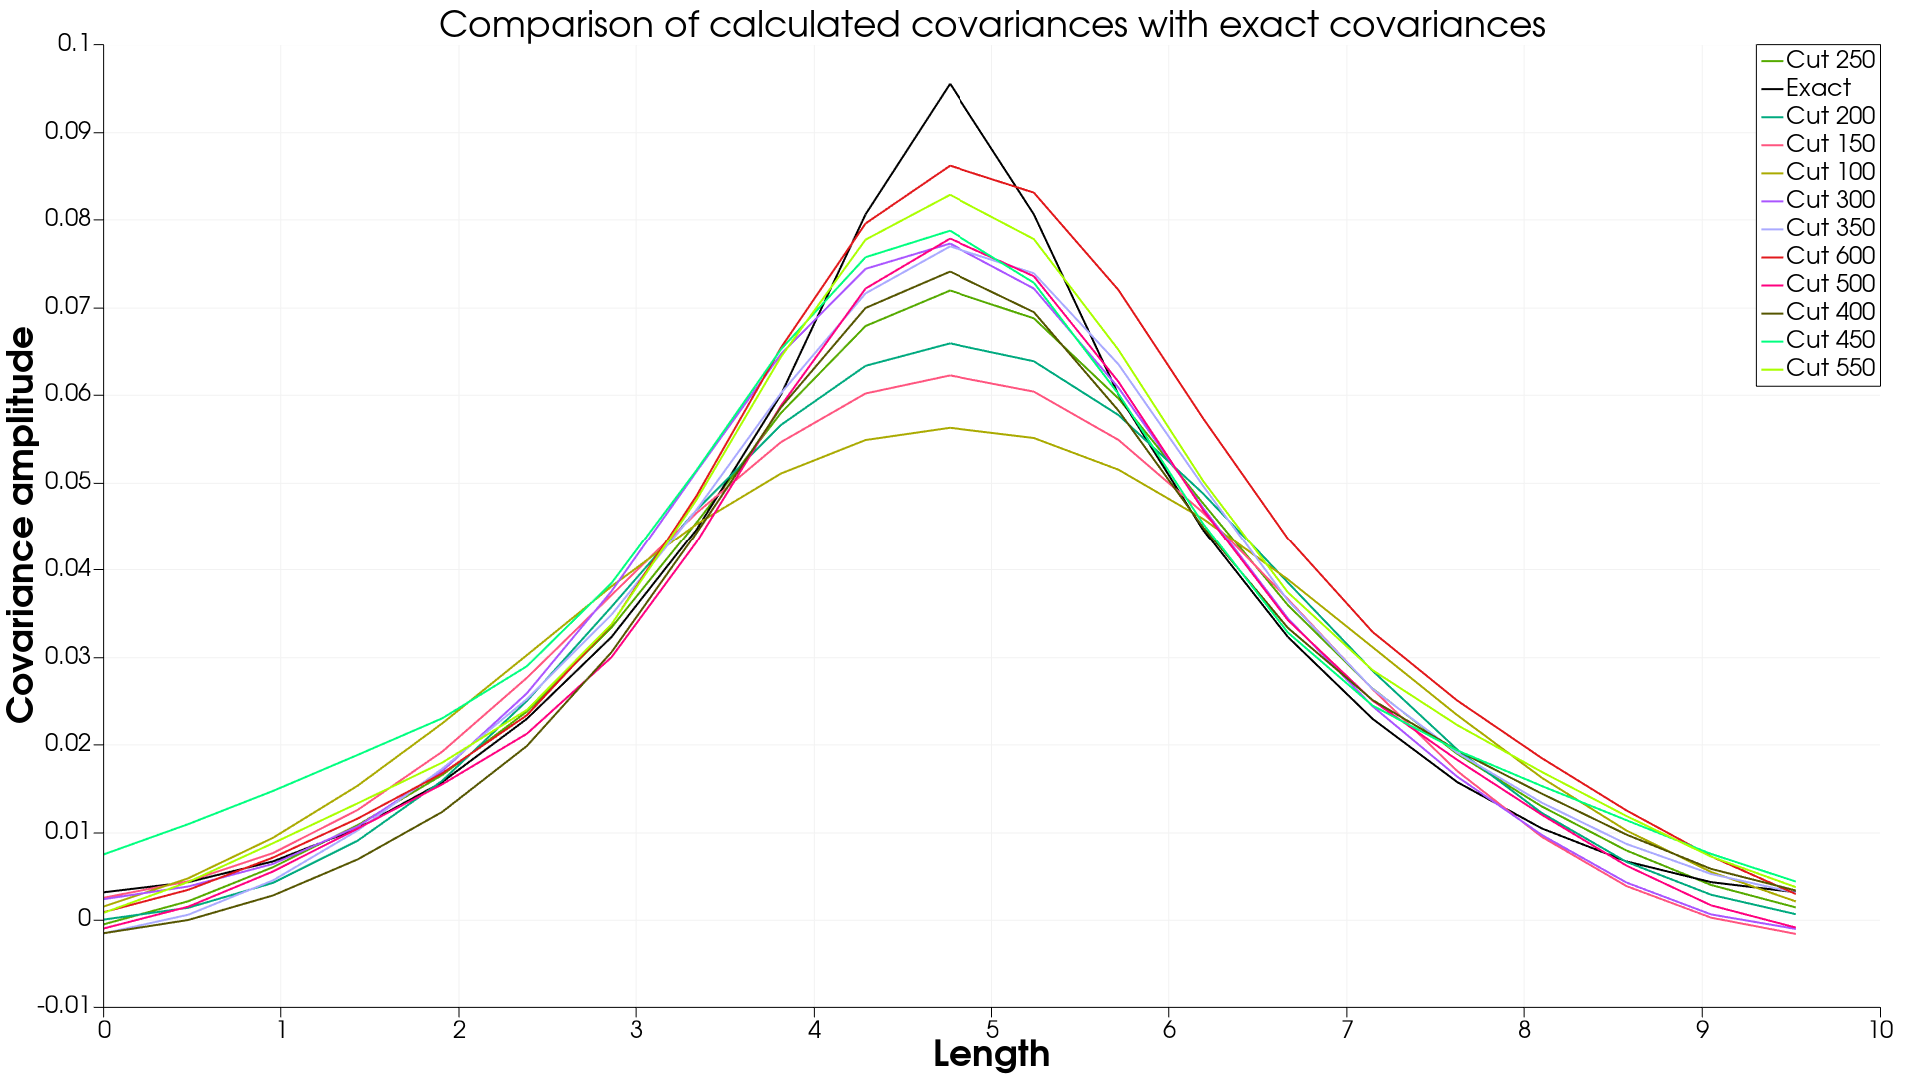
\includegraphics[width=0.4\linewidth]{comparison_covcut4_x}} \\
        \hfill
        \subcaptionbox[List-of-Figures entry]{$y$ направление\label{img:comparison_covcut4_y}} 
        {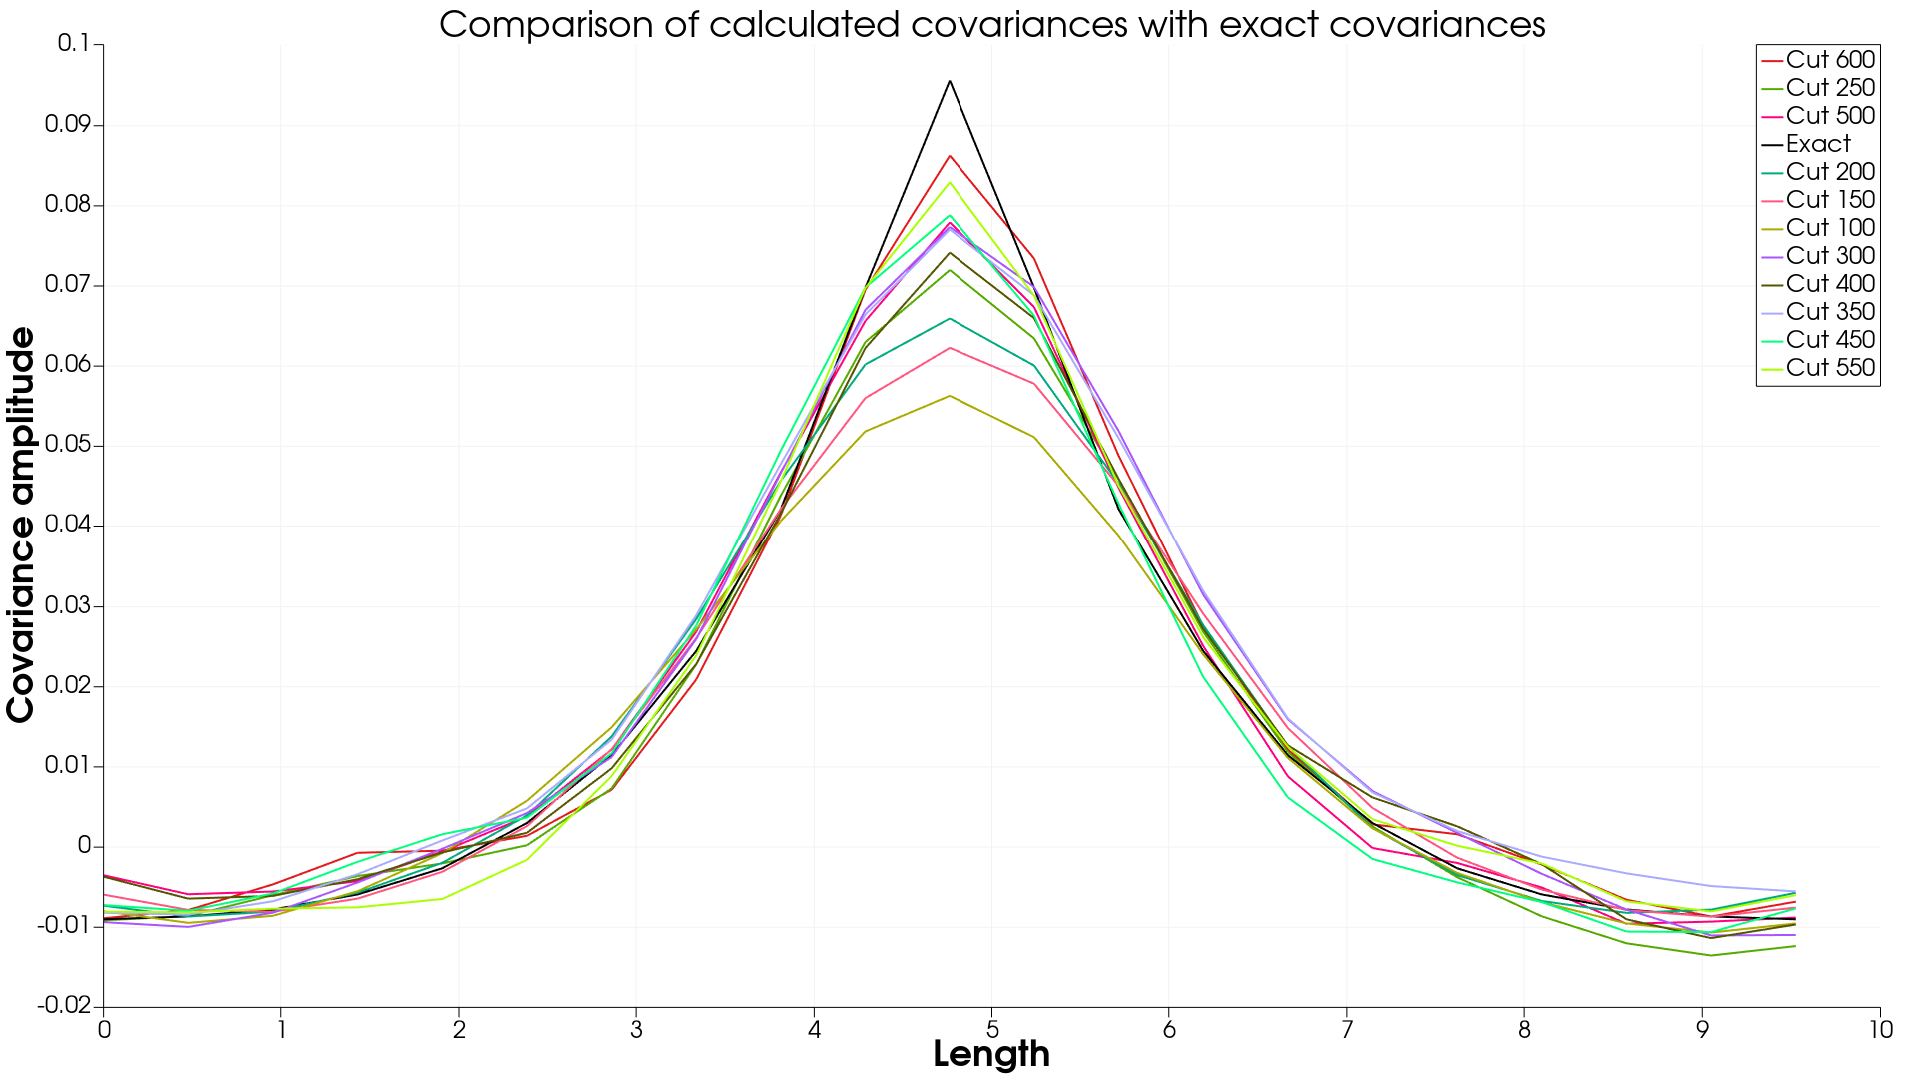
\includegraphics[width=0.4\linewidth]{comparison_covcut4_y}}%
        \hfill       
        \subcaptionbox{$z$ направление\label{img:comparison_covcut4_z}} 
        {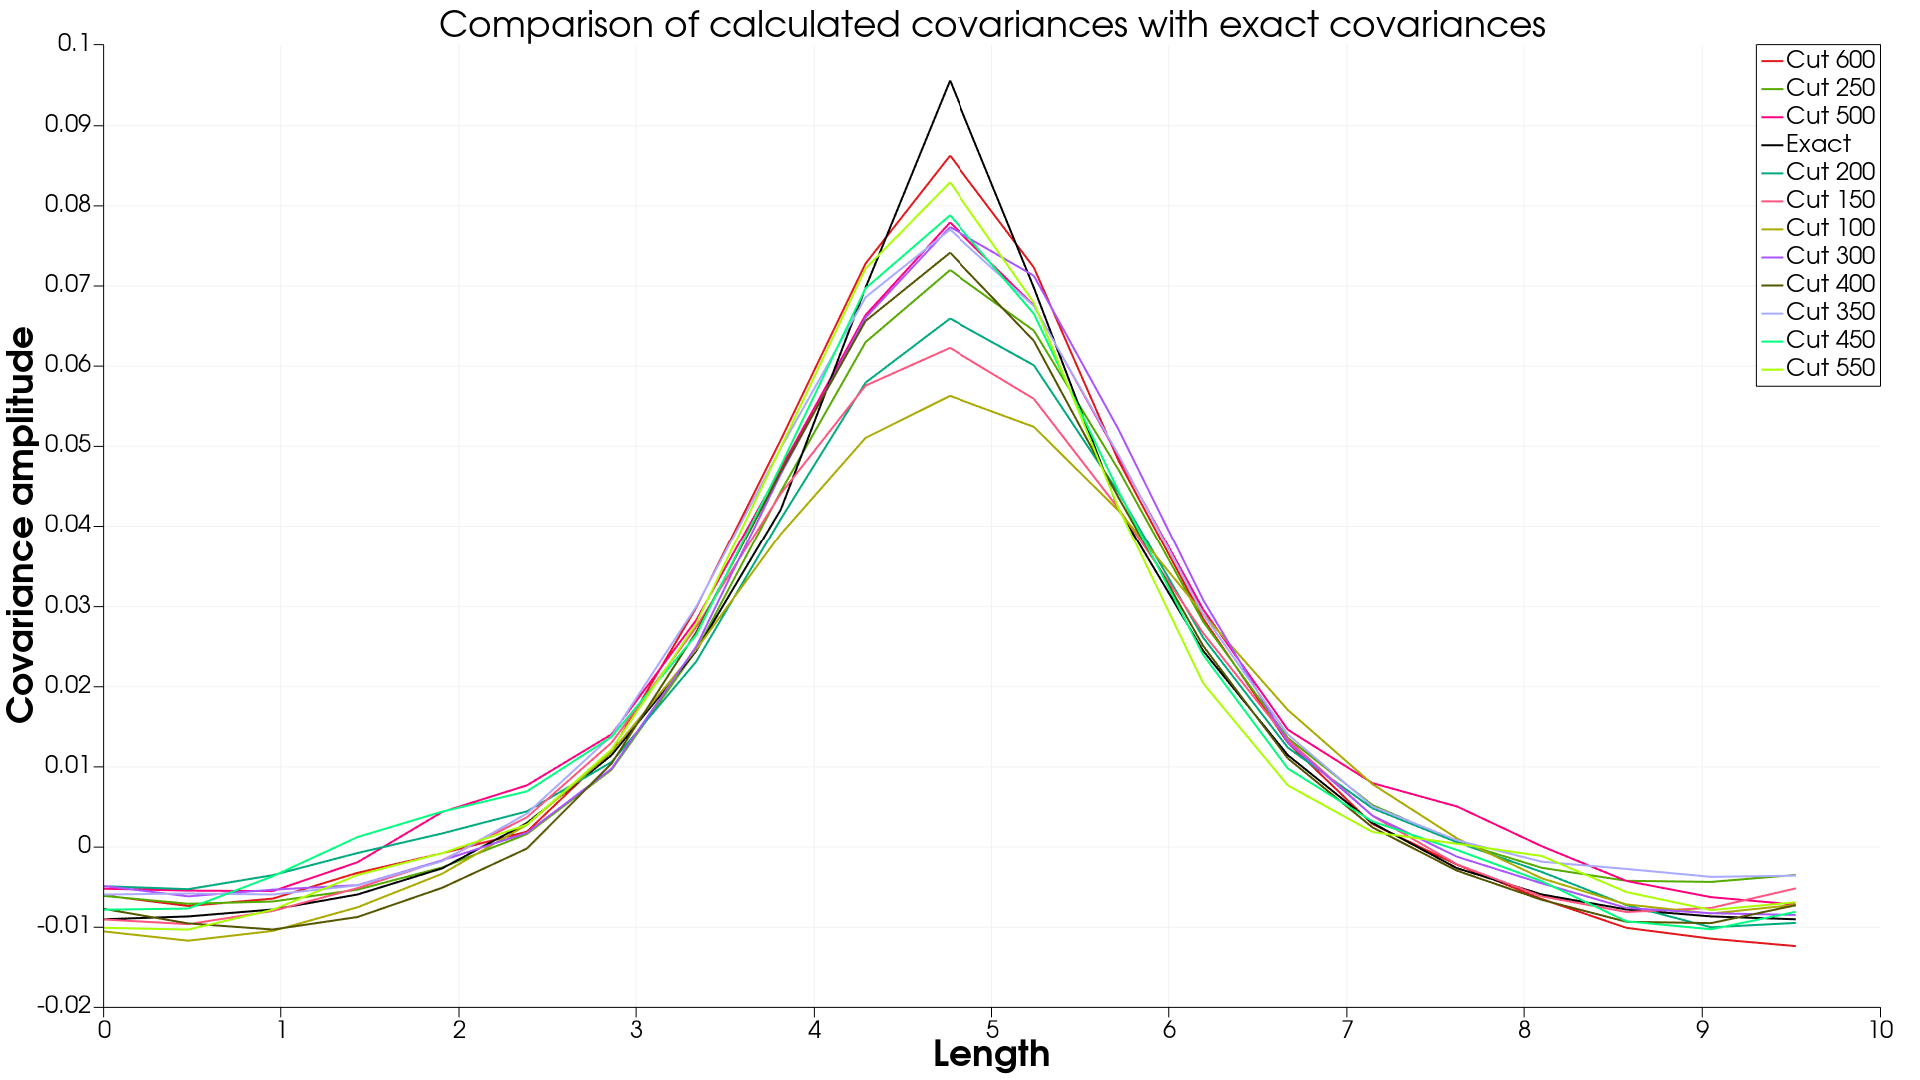
\includegraphics[width=0.4\linewidth]{comparison_covcut4_z}}
        \hfill
    }
    
    \onehalfspacing{Сравнение ковариацинной функции, допуск 4\%, для направлений а) вдоль диагонали, б) вдоль оси $x$, в) вдоль оси $y$, г) вдоль оси $z$}
    \caption{Сравнение ковариационной функции для допуска по амплитуде ковариаций в 4\% для различных направлений в рассматриваемой области}
    \label{img:covcut_4_comparison}  
\end{figure}
%
% Обрезание 5%
%
\begin{figure}[!h]
    \center{
        \hfill
        \subcaptionbox[List-of-Figures entry]{диагональ\label{img:comparison_covcut5_diag}} 
        {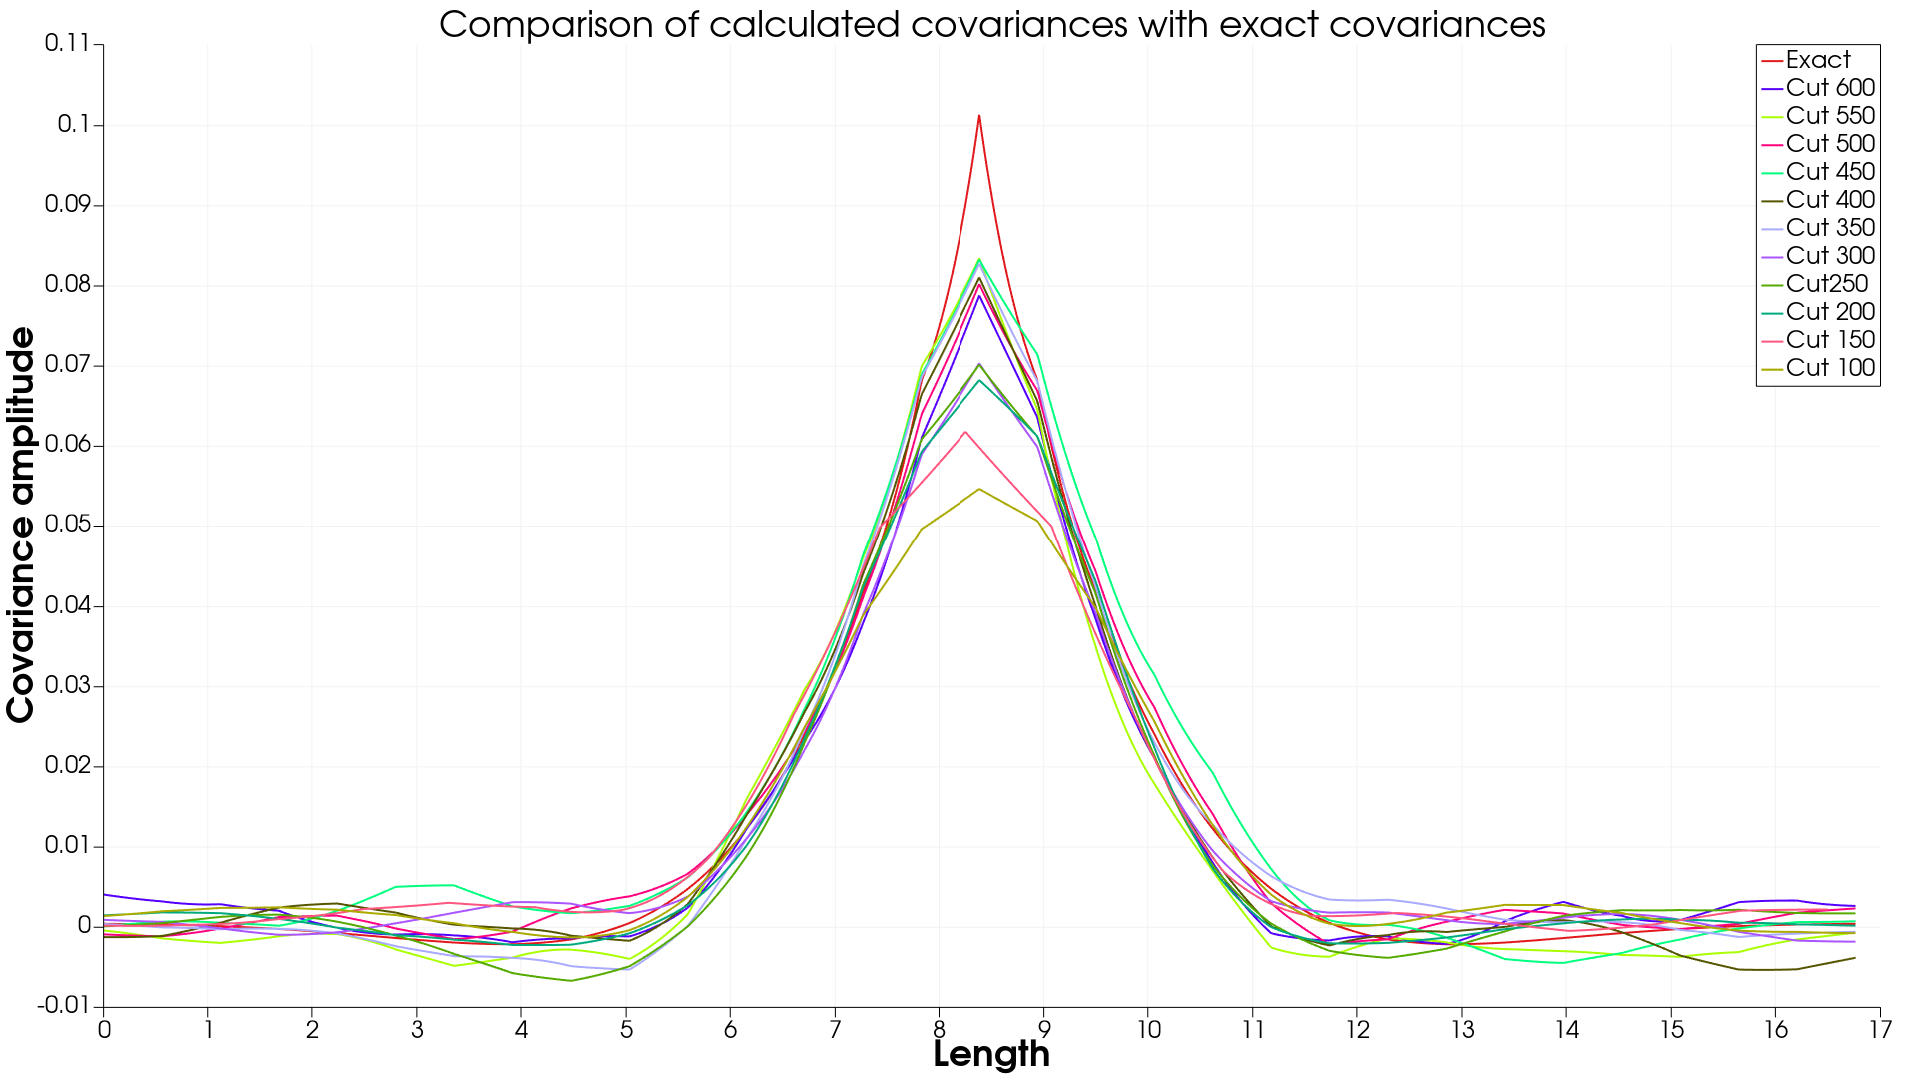
\includegraphics[width=0.4\linewidth]{comparison_covcut5_diag}}%
        \hfill       
        \subcaptionbox{$x$ направление\label{img:comparison_covcut5_x}} 
        {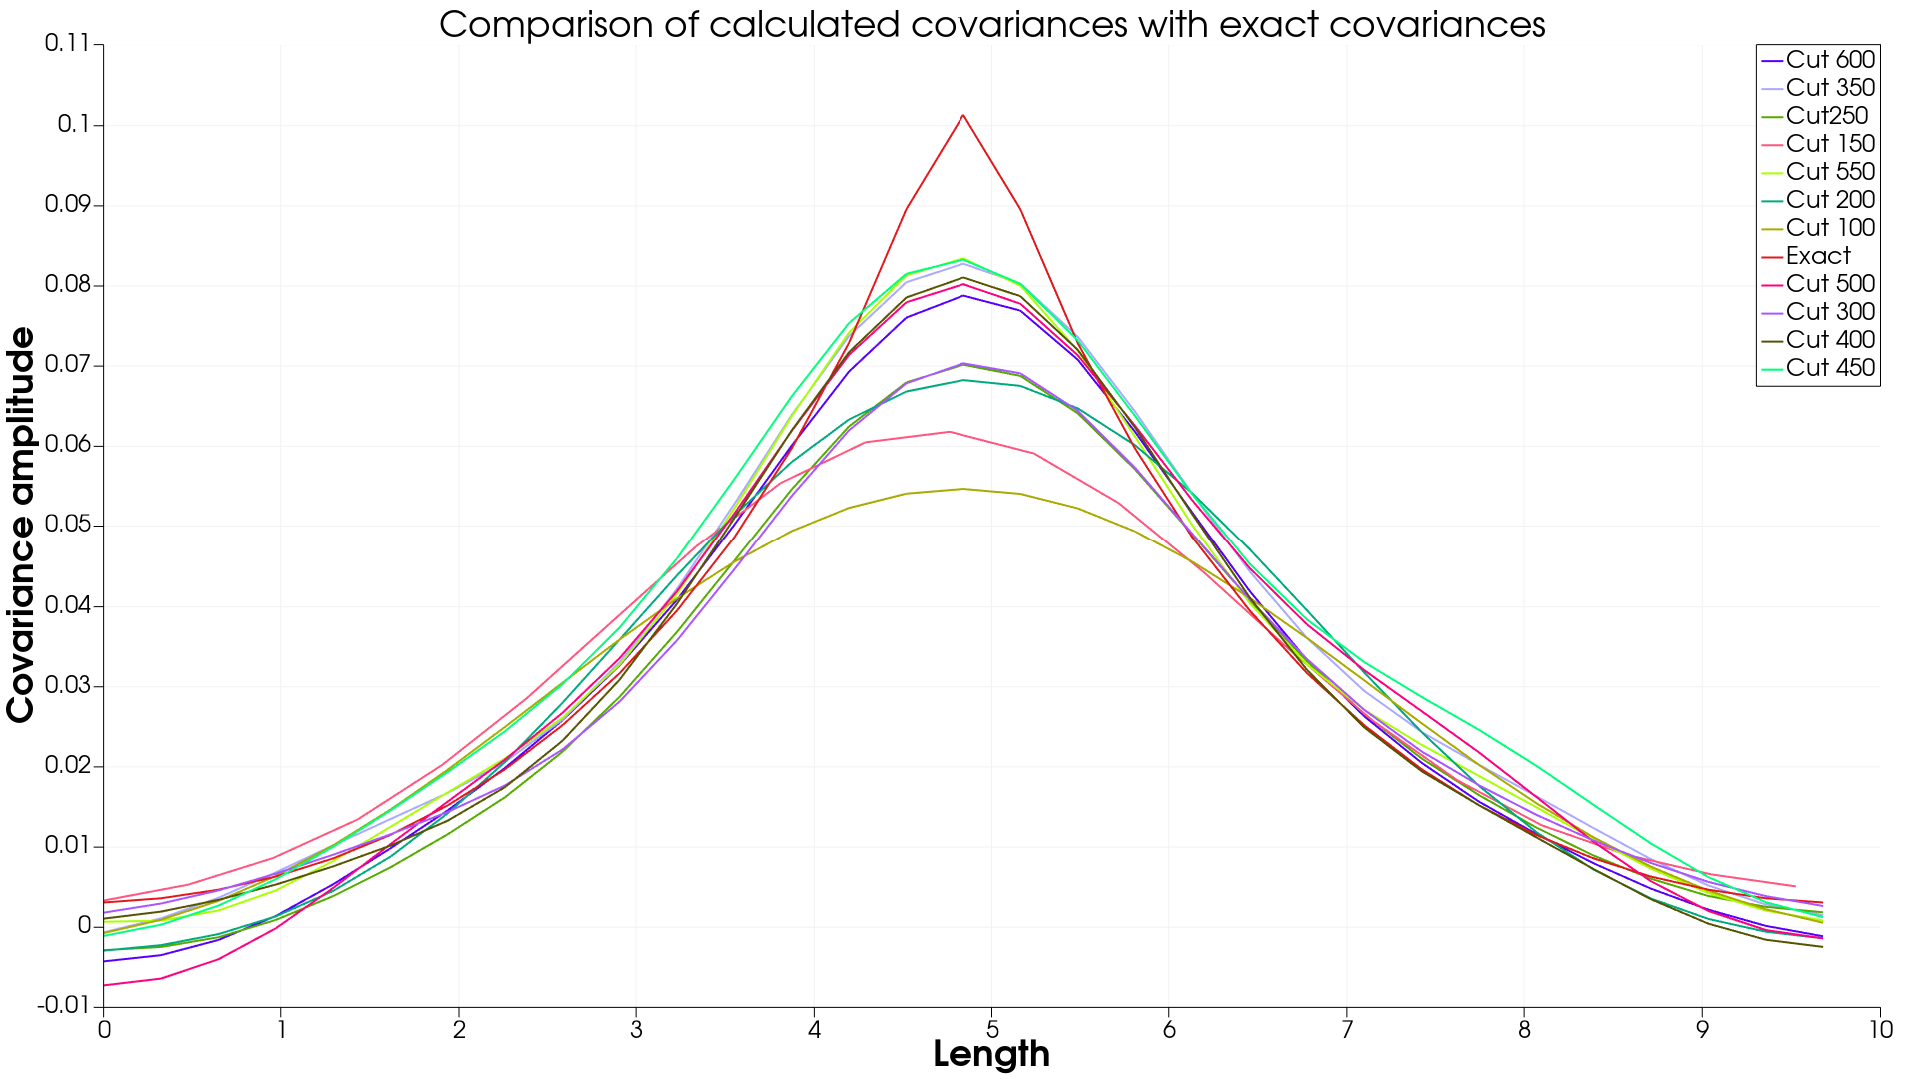
\includegraphics[width=0.4\linewidth]{comparison_covcut5_x}} \\
        \hfill
        \subcaptionbox[List-of-Figures entry]{$y$ направление\label{img:comparison_covcut5_y}} 
        {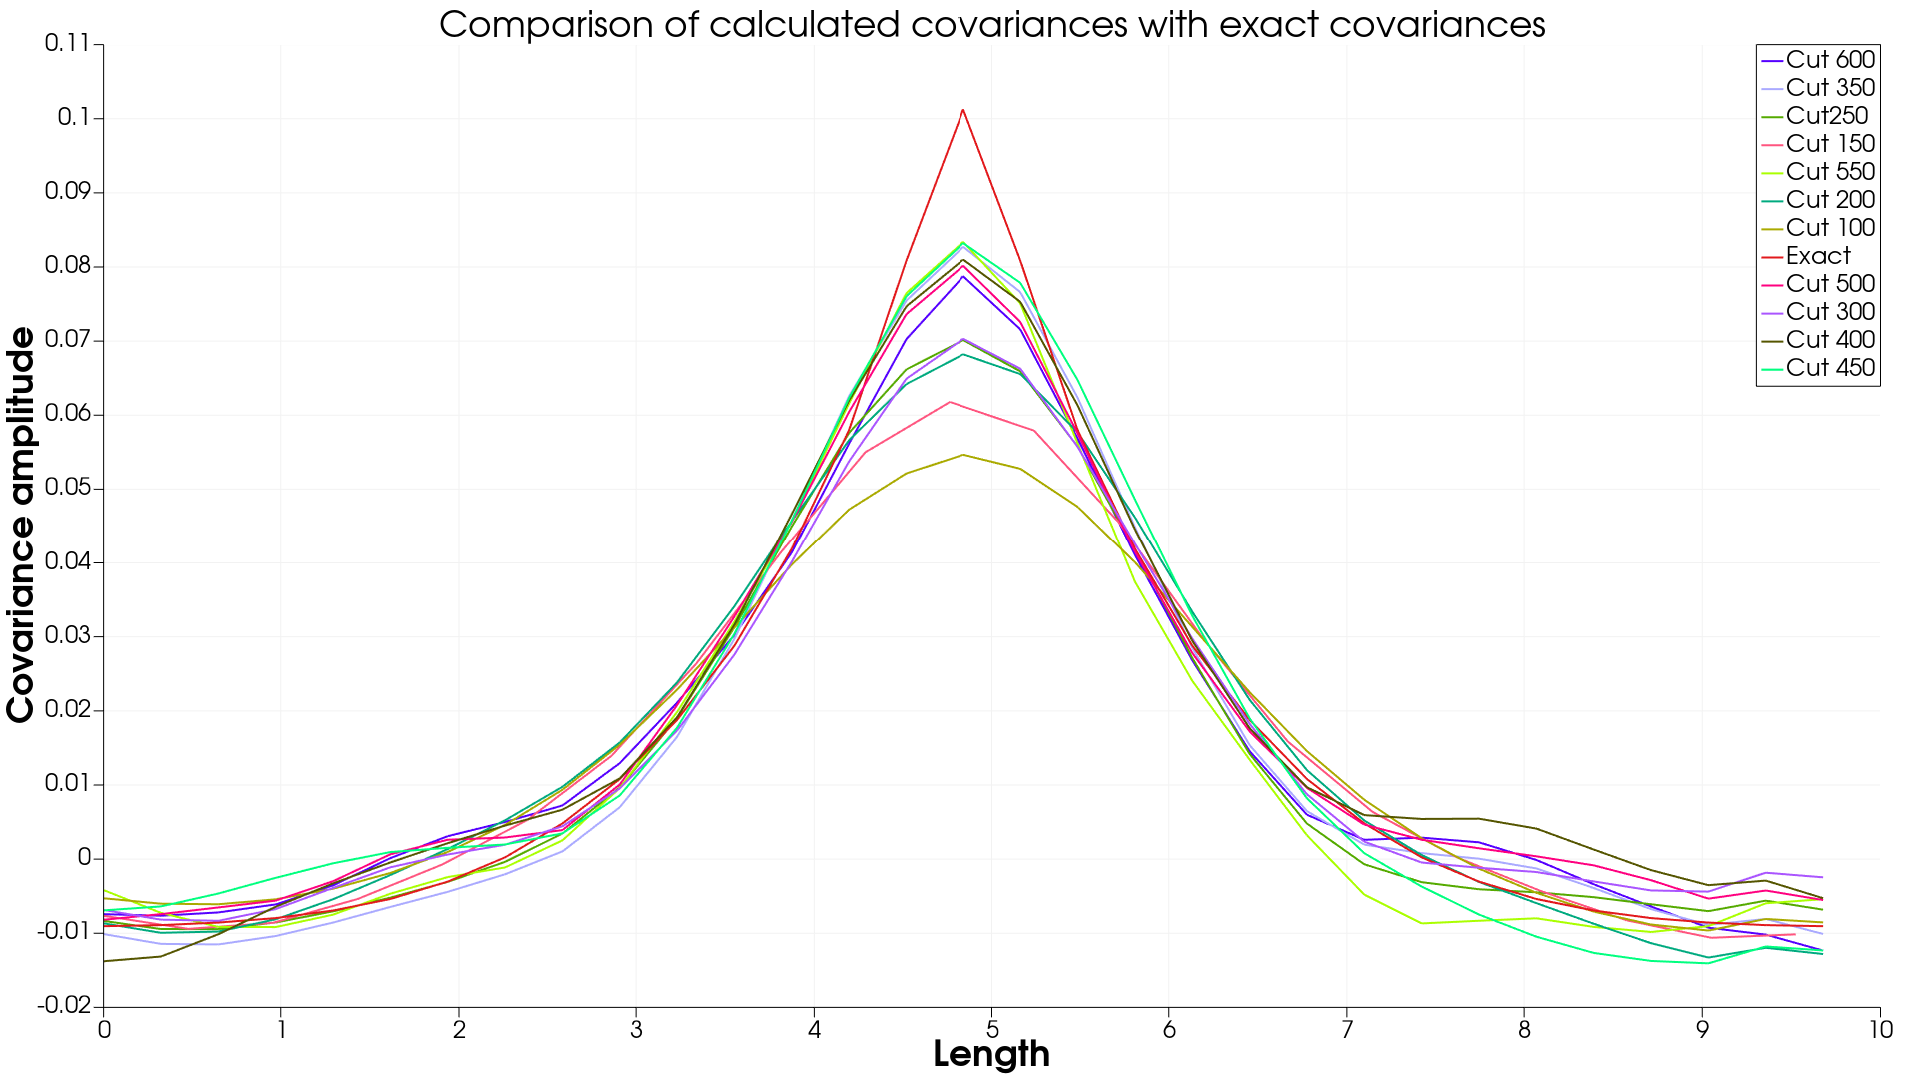
\includegraphics[width=0.4\linewidth]{comparison_covcut5_y}}%
        \hfill       
        \subcaptionbox{$z$ направление\label{img:comparison_covcut5_z}} 
        {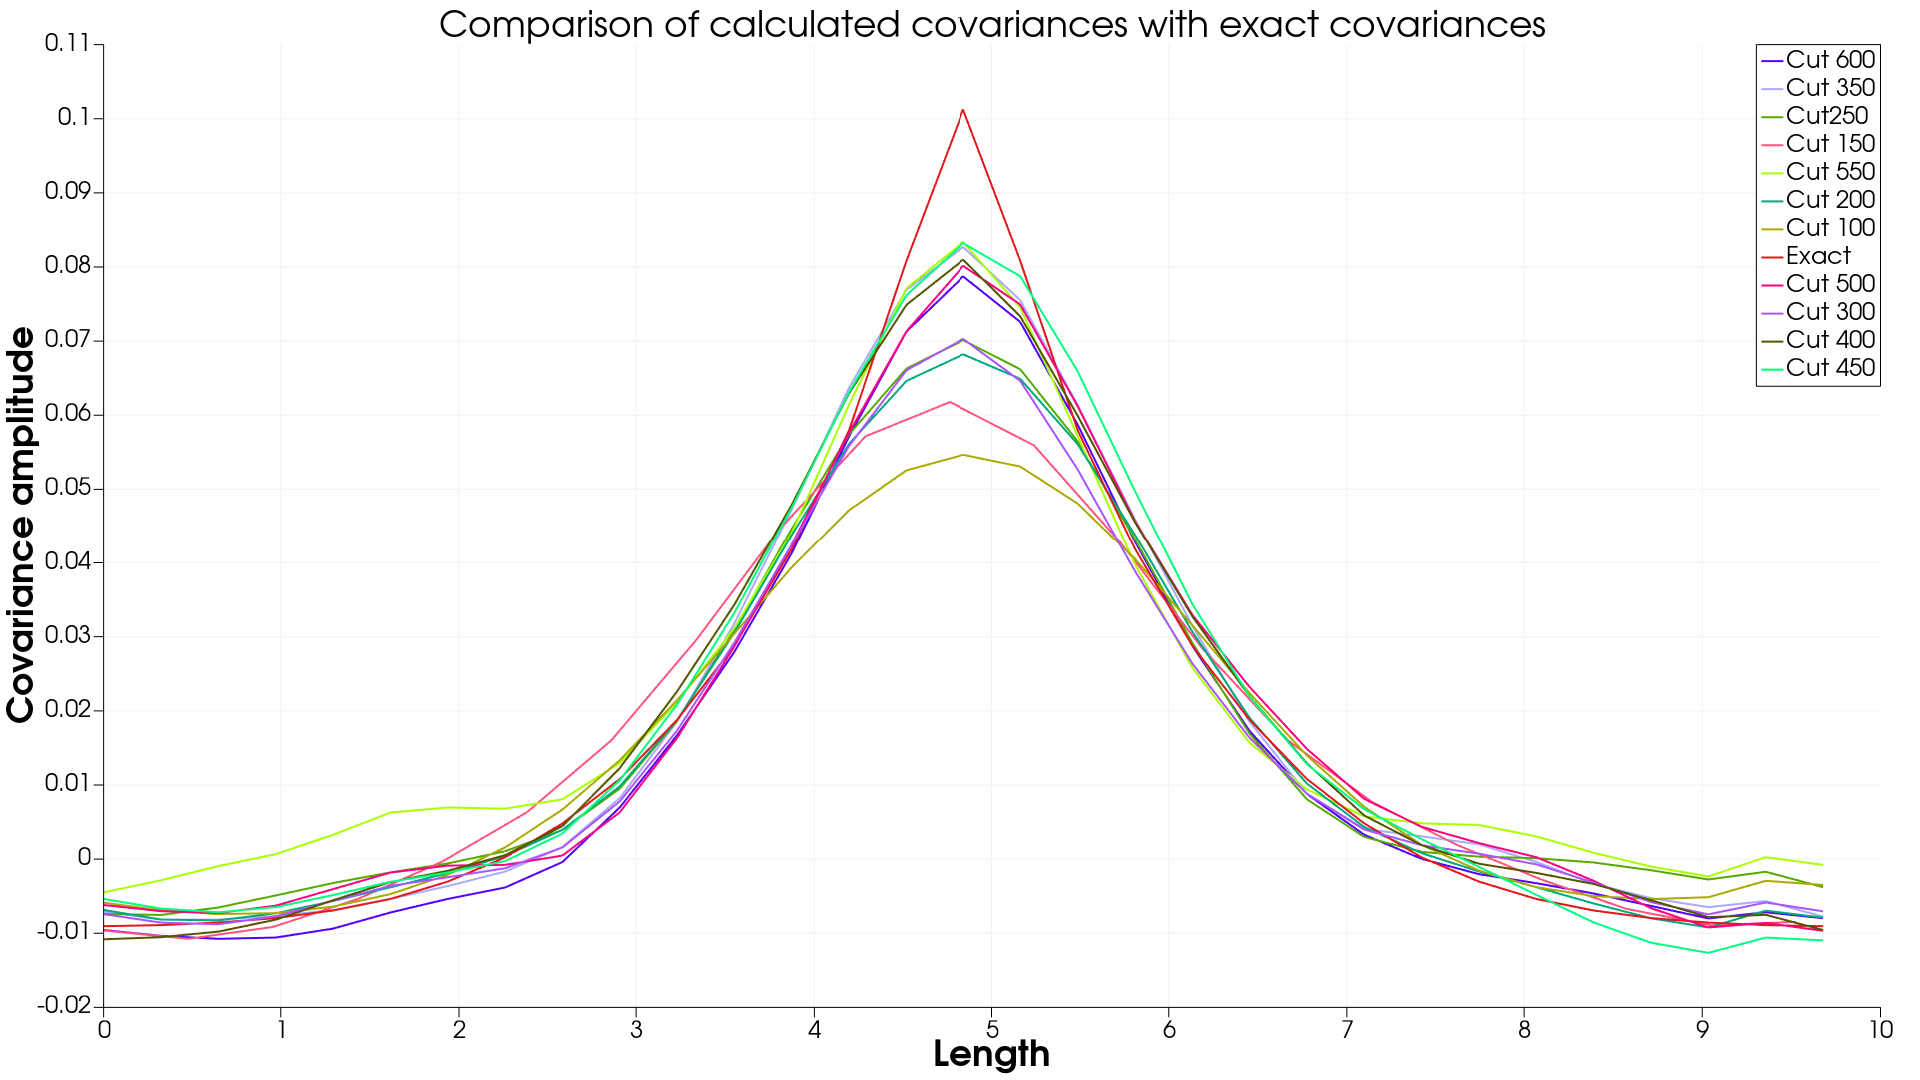
\includegraphics[width=0.4\linewidth]{comparison_covcut5_z}}
        \hfill
    }
    
    \onehalfspacing{Сравнение ковариацинной функции, допуск 5\%, для направлений а) вдоль диагонали, б) вдоль оси $x$, в) вдоль оси $y$, г) вдоль оси $z$}
    \caption{Сравнение ковариационной функции для допуска по амплитуде ковариаций в 5\% для различных направлений в рассматриваемой области}
    \label{img:covcut_5_comparison}  
\end{figure}

Так как расчёт статистических параметров, например ковариационной функции, требует какого-то набора реализаций полей скорости, необходимо также проверить, как влияет число генерируемых полей для подсчёта статистических характеристик. Это важный критерий в силу того, что основными параметрами валидации являются статистические величины. Естественно, наиболее точный случай это бесконечное число реализаций, но это также несёт в себе дополнительные временные затраты. Например, если необходимо для случая генерации поля на некоторой сетке оценить то, как хорошо метод подходит для использования на данной топологии сетки, или, например, какое число собственных значений и векторов стоит брать для последующей генерации флуктуации необходимо провести статистическое исследование, дабы не увеличивать требуемое время, стоит провести оценку некоторого оптимального числа реализаций, на котором можно проводить последующие валидации. На рисунке \ref{covcut0_eigvalues_step_samples} ниже представлены сравнение ковариационных функций, полученных в результате использования $n$ реализаций поля скоростей для подсчёта. В целом, для числа реализаций равного 1000, уже наблюдается хорошее совпадение с целевым спектром вблизи его пика, чем дальше мы отдаляемся от центра куба, тем сильнее начинает играть роль число взятых сгенерированных полей. С ростом числа взятых для расчёта реализаций также уменьшается разница между целевой ковариационной функций и рассчитанной.

\begin{figure}[!h]
    \center{
        \hfill
        \subcaptionbox[List-of-Figures entry]{диагональ\label{img:diagonal_alleigenvalues_samples_step}} 
        {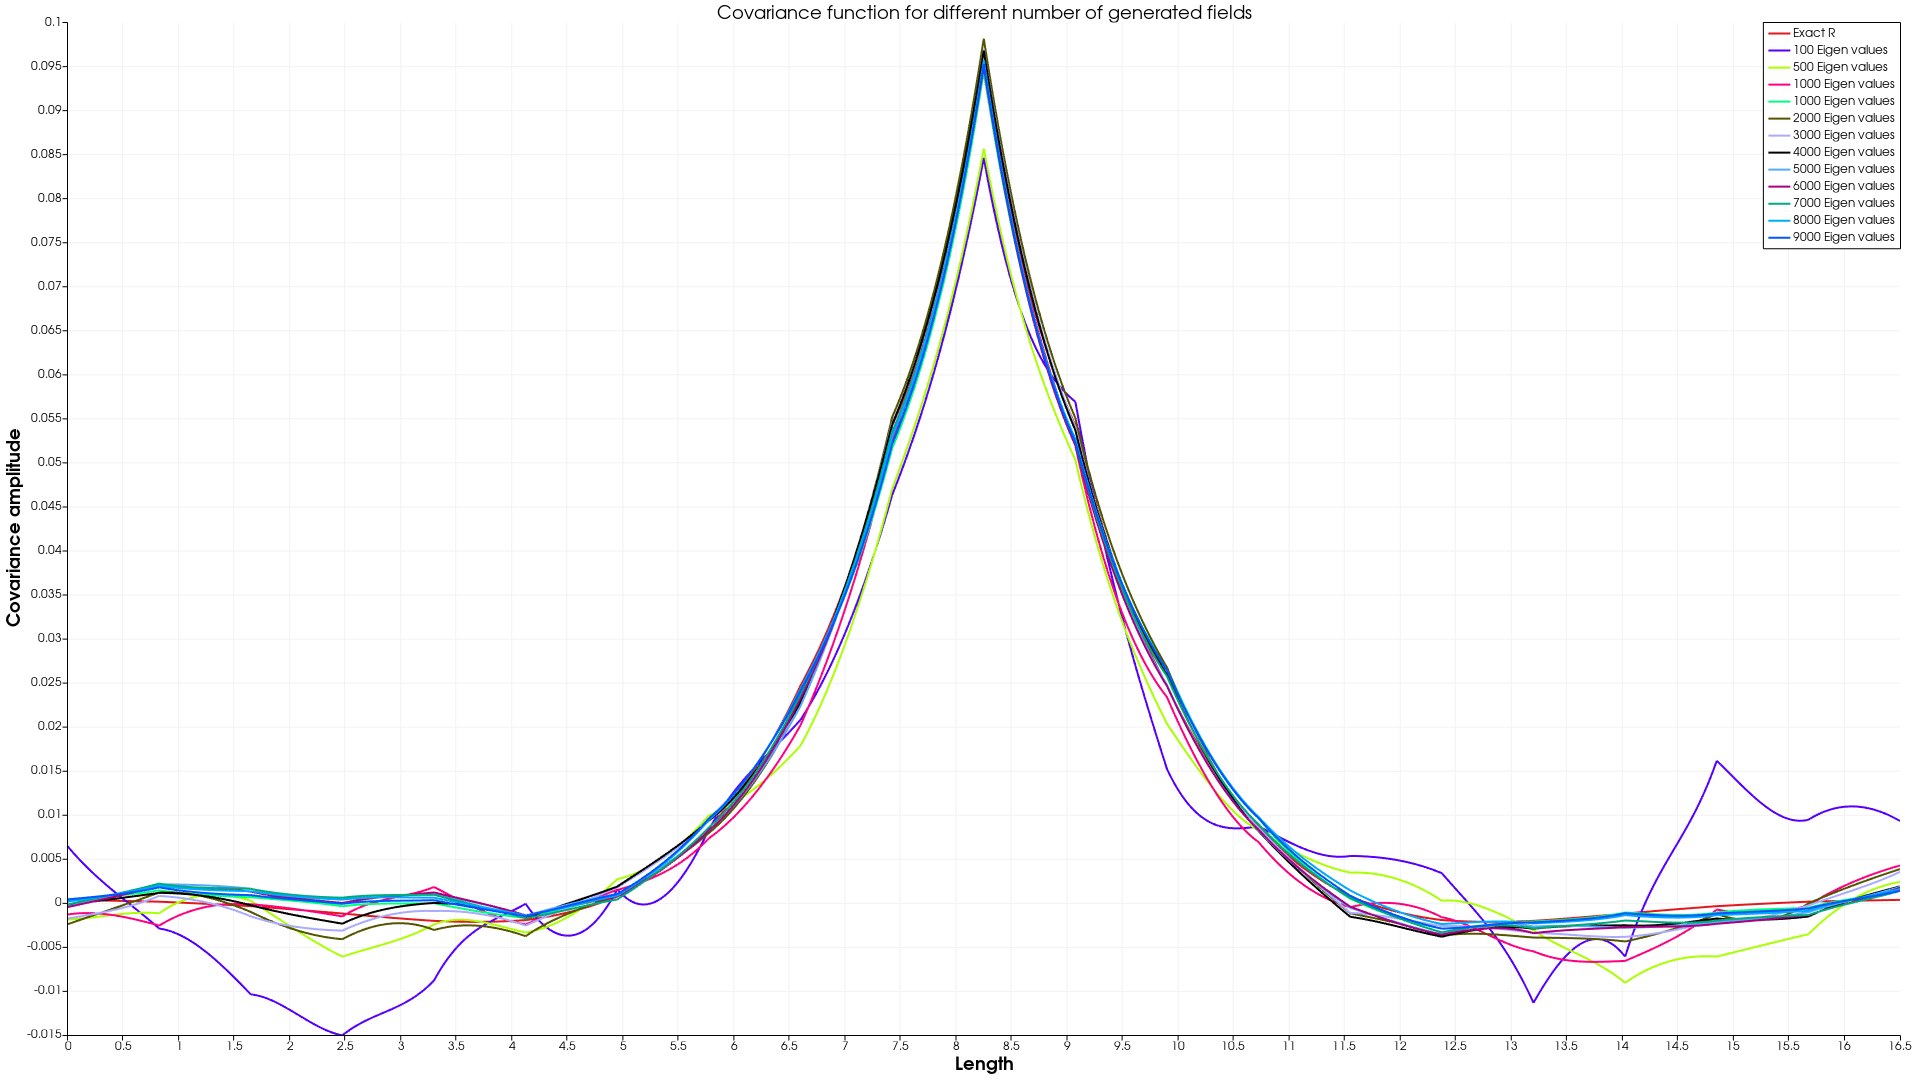
\includegraphics[width=0.4\linewidth]{diagonal_alleigenvalues_samples_step}}%
        \hfill       
        \subcaptionbox{$x$ направление\label{img:x_axis_alleigenvalues_samples_step}} 
        {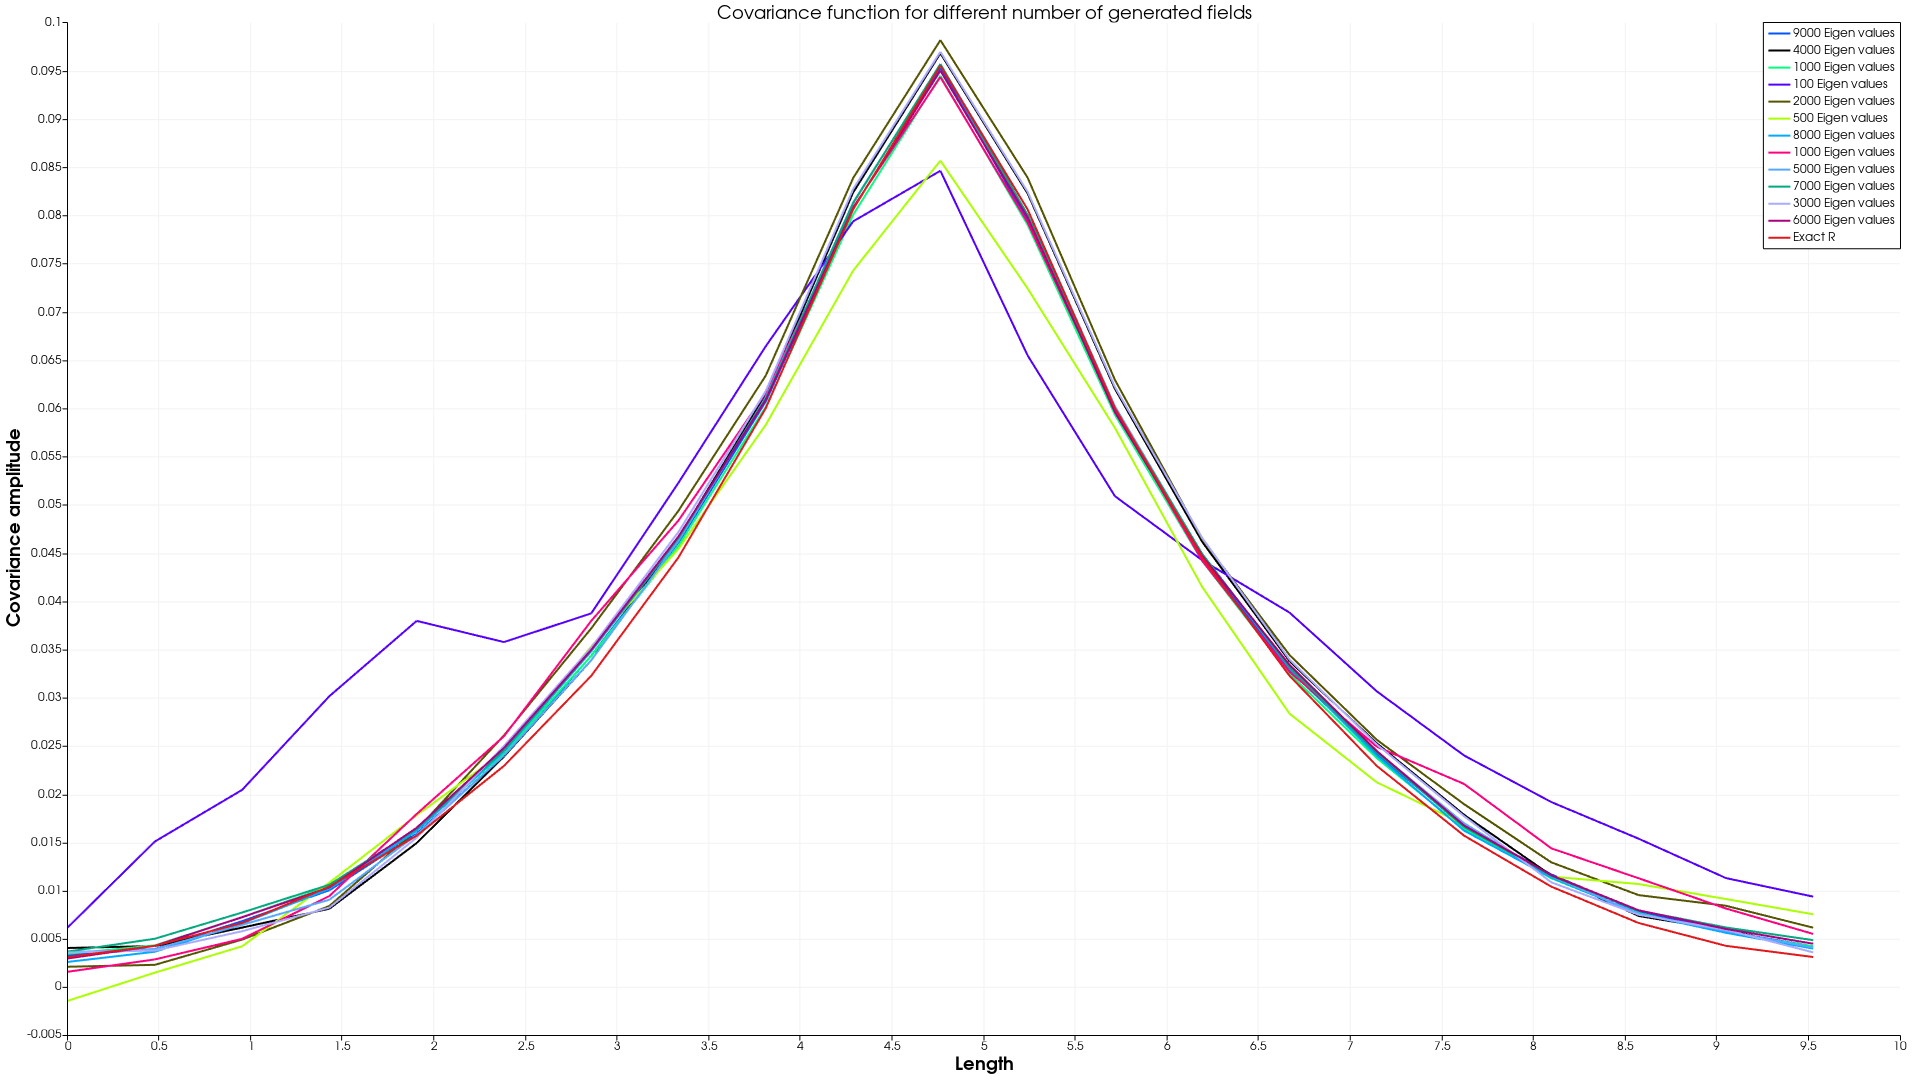
\includegraphics[width=0.4\linewidth]{x_axis_alleigenvalues_samples_step}} \\
        \hfill
        \subcaptionbox[List-of-Figures entry]{$y$ направление\label{img:y_axis_alleigenvalues_samples_step}} 
        {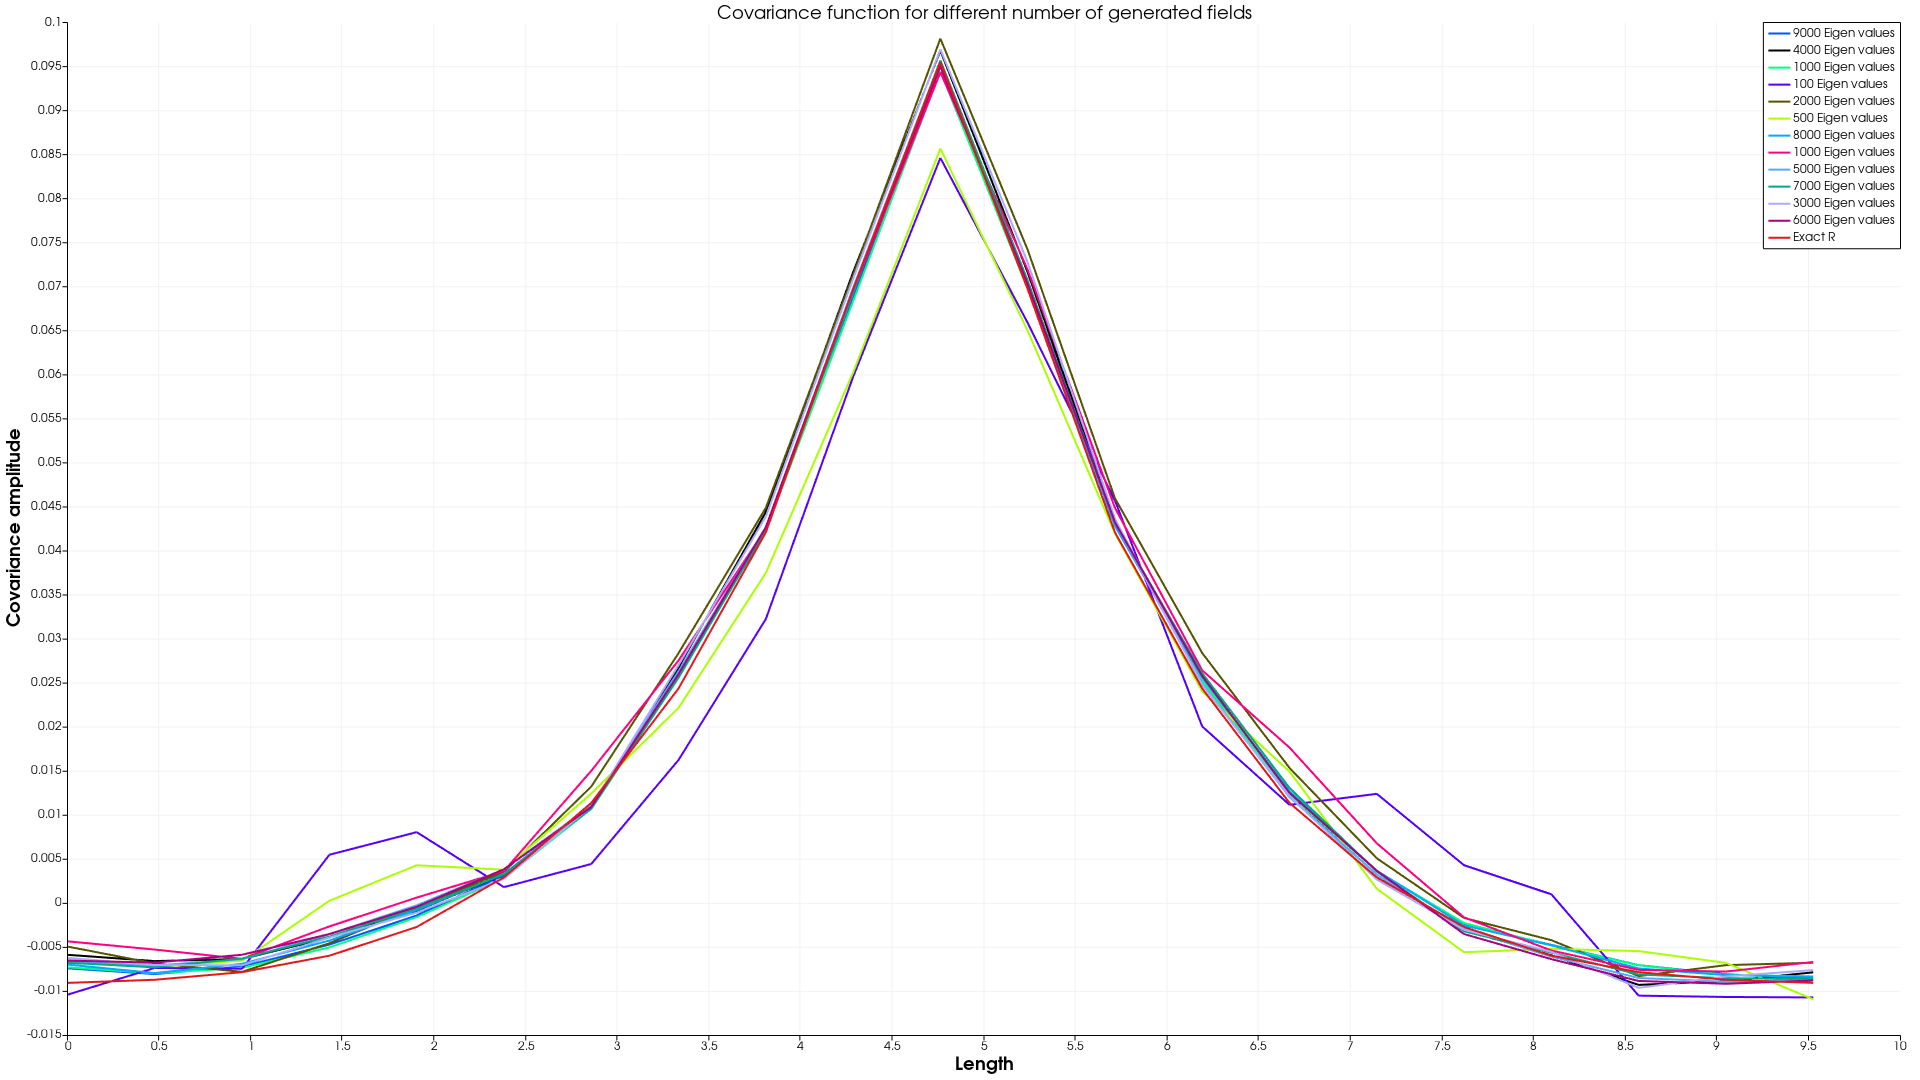
\includegraphics[width=0.4\linewidth]{y_axis_alleigenvalues_samples_step}}%
        \hfill       
        \subcaptionbox{$z$ направление\label{img:z_axis_alleigenvalues_samples_step}} 
        {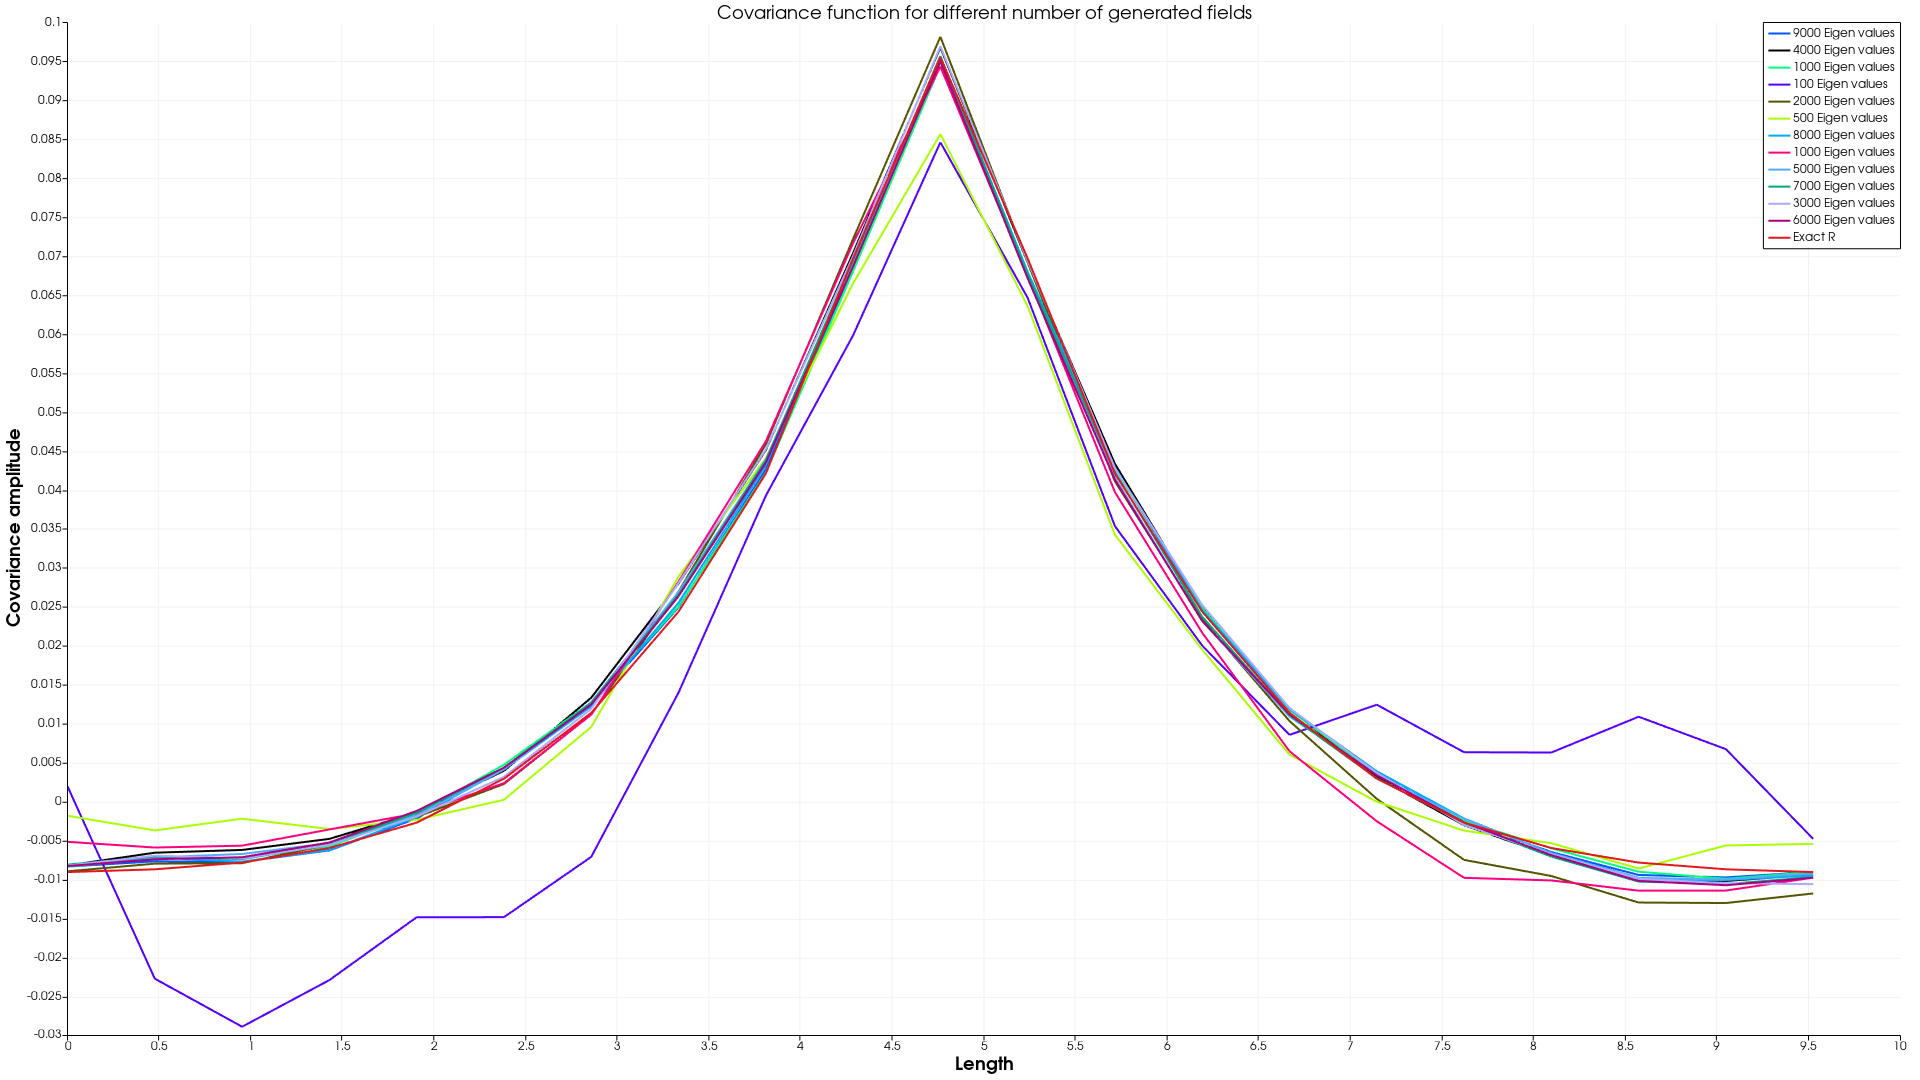
\includegraphics[width=0.4\linewidth]{z_axis_alleigenvalues_samples_step}}
        \hfill
    }
    
    \onehalfspacing{Сравнение ковариацинной функции, допуск 0\%, для направлений а) вдоль диагонали, б) вдоль оси $x$, в) вдоль оси $y$, г) вдоль оси $z$}
    \caption{Сравнение ковариационной функции для допуска по амплитуде ковариаций в 0\% для различного числа взятых реализаций полей флуктуаций для расчёта ковариационной функции в рассматриваемой области}
    \label{img:covcut0_eigvalues_step_samples}  
\end{figure}

\begin{table} [!h]%
	\caption{Величина разности между пиками для смоделированных ковариационных функций с пиком полученным из аналитического спектра преобразованием Фурье}%
	\label{tbl:peak_diff_table}
    \setlength\extrarowheight{4pt} %вот этим управляем расстоянием между рядами, \arraystretch даёт неудачный результат
    \setlength{\tymin}{1.5cm}
\begin{tabulary}{\textwidth}{@{}>{\zz}L >{\zz}C >{\zz}C >{\zz}C >{\zz}C >{\zz}C >{\zz}C@{}}
        \toprule     %%% верхняя линейка
            Число собственных значений &
            Допуск 0\% &
    	Допуск 1\% &
    	Допуск 2\% &
            Допуск 3\% &
            Допуск 4\% &
            Допуск 5\% \\
        \midrule %%% тонкий разделитель. Отделяет названия столбцов. Обязателен по ГОСТ 2.105 пункт 4.4.5 
        100 & -0.03868 & -0.04020 & -0.03814 & -0.03944  & -0.03927  & -0.0466  \\
        150 & -0.03188 & -0.03672 & -0.03047 & -0.03574  & -0.03329  & -0.03375 \\
        200 & -0.03150 & -0.02799 & -0.02830 & -0.02918  & -0.02963  & -0.03303 \\
        250 & -0.02461 & -0.02697 & -0.02748 & -0.03013  & -0.02360  & -0.03111 \\
        300 & -0.02429 & -0.02242 & -0.02693 & -0.02630  & -0.01824  & -0.03094 \\
        350 & -0.02210 & -0.02132 & -0.02638 & -0.02462  & -0.01856  & -0.01853 \\
        400 & -0.03234 & -0.01948 & -0.02341 & -0.02631  & -0.02144  & -0.02025 \\
        450 & -0.02727 & -0.02309 & -0.01800 & -0.007552 & -0.01678  & -0.01803 \\
        500 & -0.02283 & -0.02383 & -0.02184 & -0.01308  & -0.01767  & -0.02109 \\
        550 & -0.02075 & -0.02574 & -0.01990 & -0.01961  & -0.01268  & -0.01786 \\
        600 & -0.01870 & -0.01512 & -0.01590 & -0.01079  & -0.009351 & -0.02251 \\
        \midrule%%% тонкий разделитель
        \multicolumn{7}{@{}p{\textwidth}}{%
            \vspace*{-4ex}% этим подтягиваем повыше
            \hspace*{2.5em}% абзацный отступ - требование ГОСТ 2.105
            Примечание -- значения заданы до 4 значащих цифр
        }
        \\
        \bottomrule %%% нижняя линейка
    \end{tabulary}%
\end{table}

В таблице \ref{peak_diff_table} представлены значения разности между пиком точной функции и пиками для функций отвечающим различному числу взятых собственных чисел. 

\begin{table} [!h]%
	\caption{Величина $\iiint_V (R - R_{exact})^2 dV$ смоделированных ковариационных функций с пиком полученным из аналитического спектра преобразованием Фурье}%
	\label{tbl:sqr_diff_table}
    \setlength\extrarowheight{4pt} %вот этим управляем расстоянием между рядами, \arraystretch даёт неудачный результат
    \setlength{\tymin}{1.5cm}
\begin{tabulary}{\textwidth}{@{}>{\zz}L >{\zz}C >{\zz}C >{\zz}C >{\zz}C >{\zz}C >{\zz}C@{}}
        \toprule     %%% верхняя линейка
            Число собственных значений &
            Допуск 0\% &
    	Допуск 1\% &
    	Допуск 2\% &
            Допуск 3\% &
            Допуск 4\% &
            Допуск 5\% \\
        \midrule %%% тонкий разделитель. Отделяет названия столбцов. Обязателен по ГОСТ 2.105 пункт 4.4.5 
        100 & 0.005392 & 0.005629 & 0.005147 & 0.005709  & 0.005091  & 0.005871  \\
        150 & 0.004312 & 0.004123 & 0.004802 & 0.004546  & 0.004971  & 0.005351 \\
        200 & 0.004390 & 0.004272 & 0.003796 & 0.005035  & 0.005468  & 0.007215 \\
        250 & 0.004358 & 0.003895 & 0.004723 & 0.004545  & 0.006956  & 0.007789 \\
        300 & 0.004783 & 0.005905 & 0.004314 & 0.005086  & 0.006408  & 0.007328 \\
        350 & 0.005015 & 0.005662 & 0.005505 & 0.005314  & 0.007291  & 0.008133 \\
        400 & 0.005787 & 0.006087 & 0.005244 & 0.004887  & 0.006656  & 0.01095 \\
        450 & 0.005369 & 0.004789 & 0.005936 & 0.007729  & 0.006879  & 0.009317 \\
        500 & 0.004492 & 0.004212 & 0.004497 & 0.006602  & 0.006941  & 0.007891 \\
        550 & 0.004914 & 0.004454 & 0.004986 & 0.005357  & 0.008319  & 0.01020 \\
        600 & 0.004977 & 0.007869 & 0.006807 & 0.007966  & 0.008000  & 0.007966 \\
        \midrule%%% тонкий разделитель
        \multicolumn{7}{@{}p{\textwidth}}{%
            \vspace*{-4ex}% этим подтягиваем повыше
            \hspace*{2.5em}% абзацный отступ - требование ГОСТ 2.105
            Примечание -- значения заданы до 4 значащих цифр
        }
        \\
        \bottomrule %%% нижняя линейка
    \end{tabulary}%
\end{table}

В таблице \ref{integrals_for_samples_step} представлены характеристики характеризующие близость расчётной ковариационной функции с точной. Как говорилось ранее, для 1000 реализаций уже наблюдается хорошее соответствие, таким образом для быстрой оценки, вполне может хватить взятия 1000 модельных полей. Как можно видеть разница между пиковыми значениями достаточно сильно изменяется и в данном случае не в полной мере характеризует точность расчёта статистики, это следует из того факта, что интегральное значение квадрата разности расчётной и аналитической функций уменьшается с ростом числа взятых реализаций, что является более жестким критерием близости двух функций. При числе взятых реализаций в районе 5000-6000 наблюдается наибольший баланс между обеими характеристиками. Также, примерно при этих же значениях разность между двумя функциями начинает уменьшаться более медленно. В общем для получения приемлемой оценки статистических параметров за наилучшее время стоит проводить статистический анализ на количестве реализаций в районе 5000.

\begin{table} [!h]%
	\caption{Интегральные величины характеризующие точность рассчитываемых статистических характеристик}%
	\label{tbl:integrals_for_samples_step}
    \setlength\extrarowheight{4pt} %вот этим управляем расстоянием между рядами, \arraystretch даёт неудачный результат
    \setlength{\tymin}{1.5cm}
    \begin{tabulary}{\textwidth}{@{}>{\zz}L >{\zz}C >{\zz}C@{}}
        \toprule     %%% верхняя линейка
            Число реализаций &
            Разница между пиками &
    	$\iiint_V (R - R_{exact})^2 dV$ \\
        \midrule %%% тонкий разделитель. Отделяет названия столбцов. Обязателен по ГОСТ 2.105 пункт 4.4.5 
      100               &       -0.01090   &       0.06227 \\
      500               &       -0.00985   &       0.01167 \\
      1000              &       -0.00119   &       0.00697 \\
      2000              &       0.002638    &       0.003698 \\ 
      3000              &       0.001430    &       0.002393 \\ 
      4000              &       0.001282   &       0.001941 \\ 
      5000              &       0.000118  &       0.001532 \\
      6000              &       -0.00052  &       0.001211 \\ 
      7000              &       0.000171  &       0.001097 \\ 
      8000              &       0.000160   &       0.0009520 \\ 
      9000              &       -0.00025  &       0.0008152 \\ 
     10000              &       -0.00104   &       0.0007344 \\
        \midrule%%% тонкий разделитель
        \multicolumn{3}{@{}p{\textwidth}}{%
            \vspace*{-4ex}% этим подтягиваем повыше
            \hspace*{2.5em}% абзацный отступ - требование ГОСТ 2.105
            Примечание -- значения заданы до 4 значащих цифр
        }
        \\
        \bottomrule %%% нижняя линейка
    \end{tabulary}%
\end{table}

Как можно видеть из таблиц \ref{tbl:peak_diff_table} и \ref{tbl:sqr_diff_table}, а также рисунков \ref{img:covcut_0_comparison}, \ref{img:covcut_1_comparison}, \ref{img:covcut_2_comparison}, \ref{img:covcut_3_comparison}, \ref{img:covcut_4_comparison}, \ref{img:covcut_5_comparison} нет чётких значений параметров для которых наблюдается наилучшее соотношение сходимости между численным и точным графиками ковариационной функции. Также стоит отметить, что при проведении численных экспериментов наблюдались отрицательные собственные числа, которые были отброшены при дальнейших расчётах так как их число на фоне общего числа собственных чисел достаточно мало.

Перейдем к рассмотрению генерации турбулентных флуктуаций с применением кокригинга для стохастического метода. Как было описано в \ref{sect1_3} и в отличие от ранее рассмотренного одномерного подхода, необходимо иметь тензоры спектра скоростей и ковариаций. Используется подход в сборке матриц ковариаций в которой отдельные элементы отвечают за отдельные компоненты скоростей.

При построении тензоров задавалась их симметричность. Связано это с текущим рассмотрение в данной работе однородной и изотропной турбулентности. В более общем случае тензор пространственной ковариации несимметричен. Также симметричность требуется из определения тензора спектра скоростей. Так как метод требует построения глобальной матрицы, а также нахождения её собственных значений и собственных векторов мы немного экономим память для алгоритма, тем самым имея возможность, например, сгустить сетку, либо взять большее число собственных значений и векторов.

Целевой спектр задается в следующем виде

\[
    E(k) = \left\{
    \begin{alignedat}{2}
        &k^2, \quad &\text{eсли } x\leqslant 0 \\
        &k^{\frac{5}{3}}, \quad & \text{eсли } 0 < k < 3 \\
        &k^{-3}, k \geqslant 3 \\
    \end{alignedat}
    \right.
\]

Как и при рассмотрении спектрального метода, также используется вычислительная область в виде куба, центрированного в начале координат со стороной $l=10$, как для пространства Фурье, так и для физического пространства. Опорное волновое число в задаче $k_0=\frac{\pi}{5}$.  

Рассмотрим качественно получаемое поле флуктуаций. Ниже представлены полное сгенерированное поле скоростей, а также поле на срезе в плоскости $xy$ при $z = 0$, под различными углами. Наблюдаются как большие вихревые структуры, так и меньшие. Так как пик задаваемого спектра находится при $k \approx 1.0$ мы можем оценить средний размер генерируемых вихрей $ l = \frac{2 pi}{k} \approx \approx 2 \pi$, тем самым мы можем примерно выделить преобладающие вихри. Цветом представлена амплитуда вектора флуктуации, наибольшая амплитуда флуктуаций $v_{max} = 6.25$, наименьшая $v_{max} = 0.055$.  

\begin{figure}[!h]
    \center{
        \hfill
        \subcaptionbox[List-of-Figures entry]{Полное сгенерированное поле\label{img:full_cube_field}} 
        {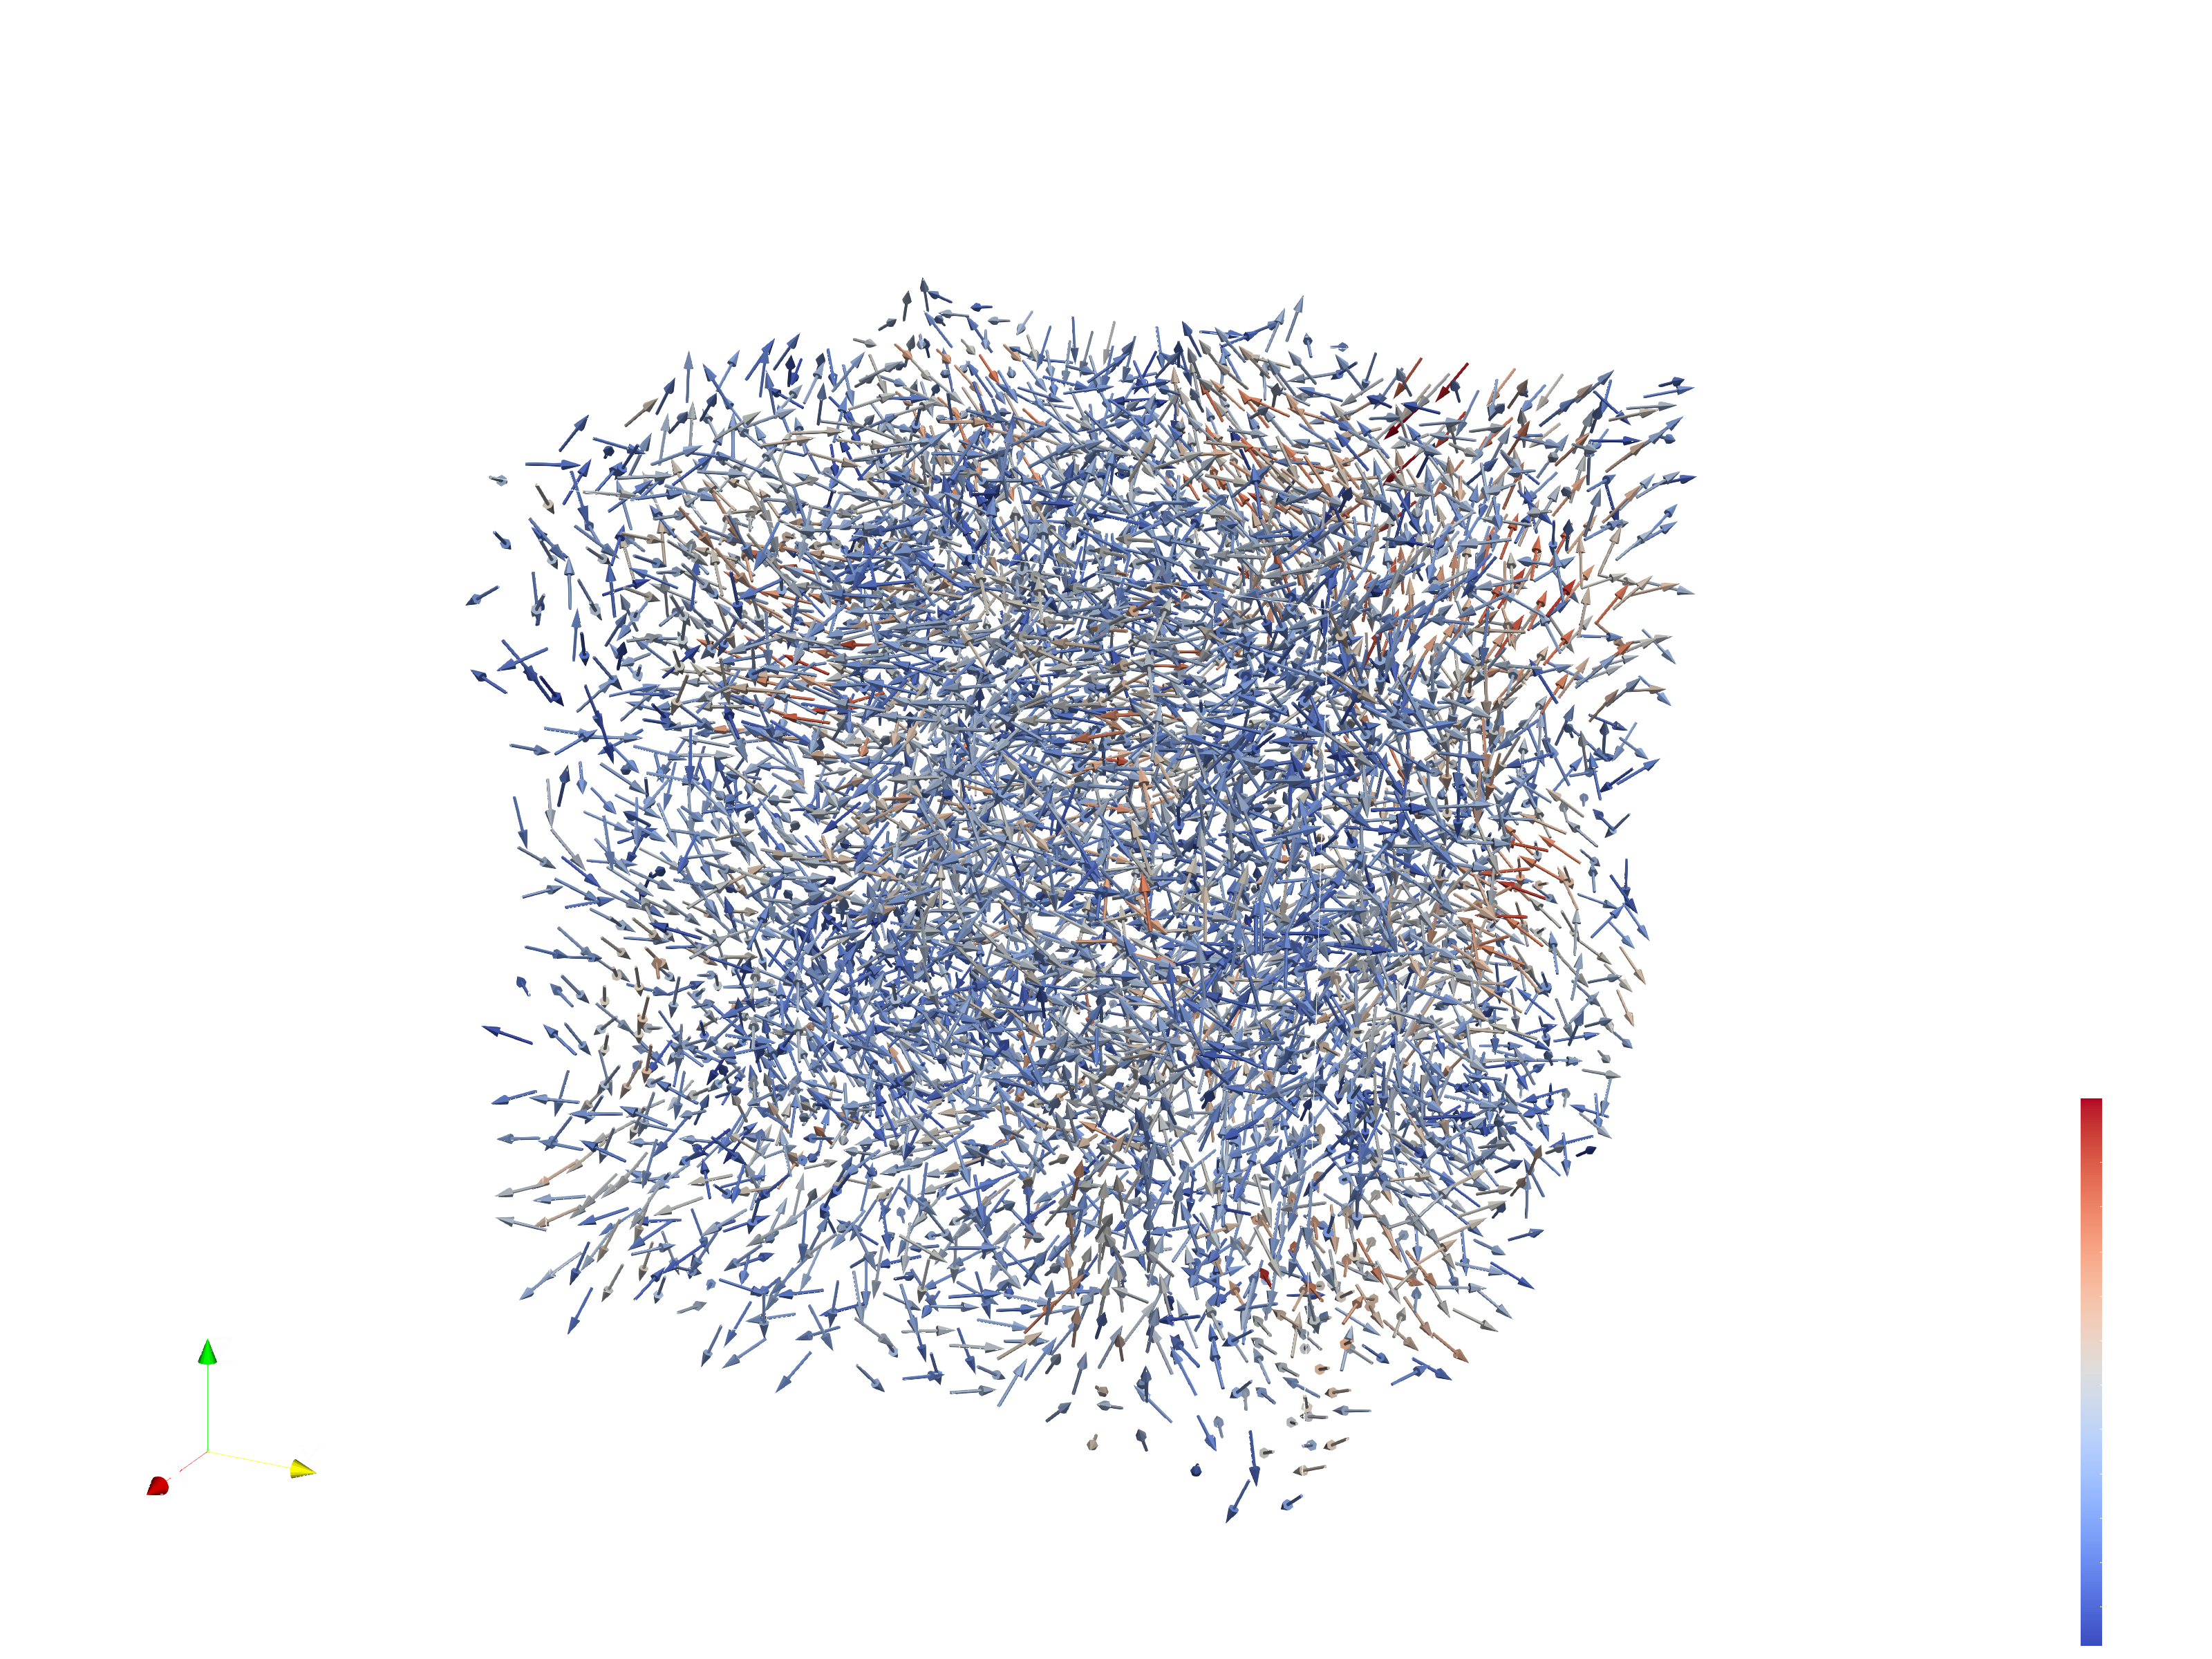
\includegraphics[width=0.4\linewidth]{images/kriging/3components/full_field_velocity_field.png}}%
        \hfill       
        \subcaptionbox{плоскость $xy$, $z = 0$\label{img:slice_velcotiy_field_xy_znormal_angle_1}} 
        {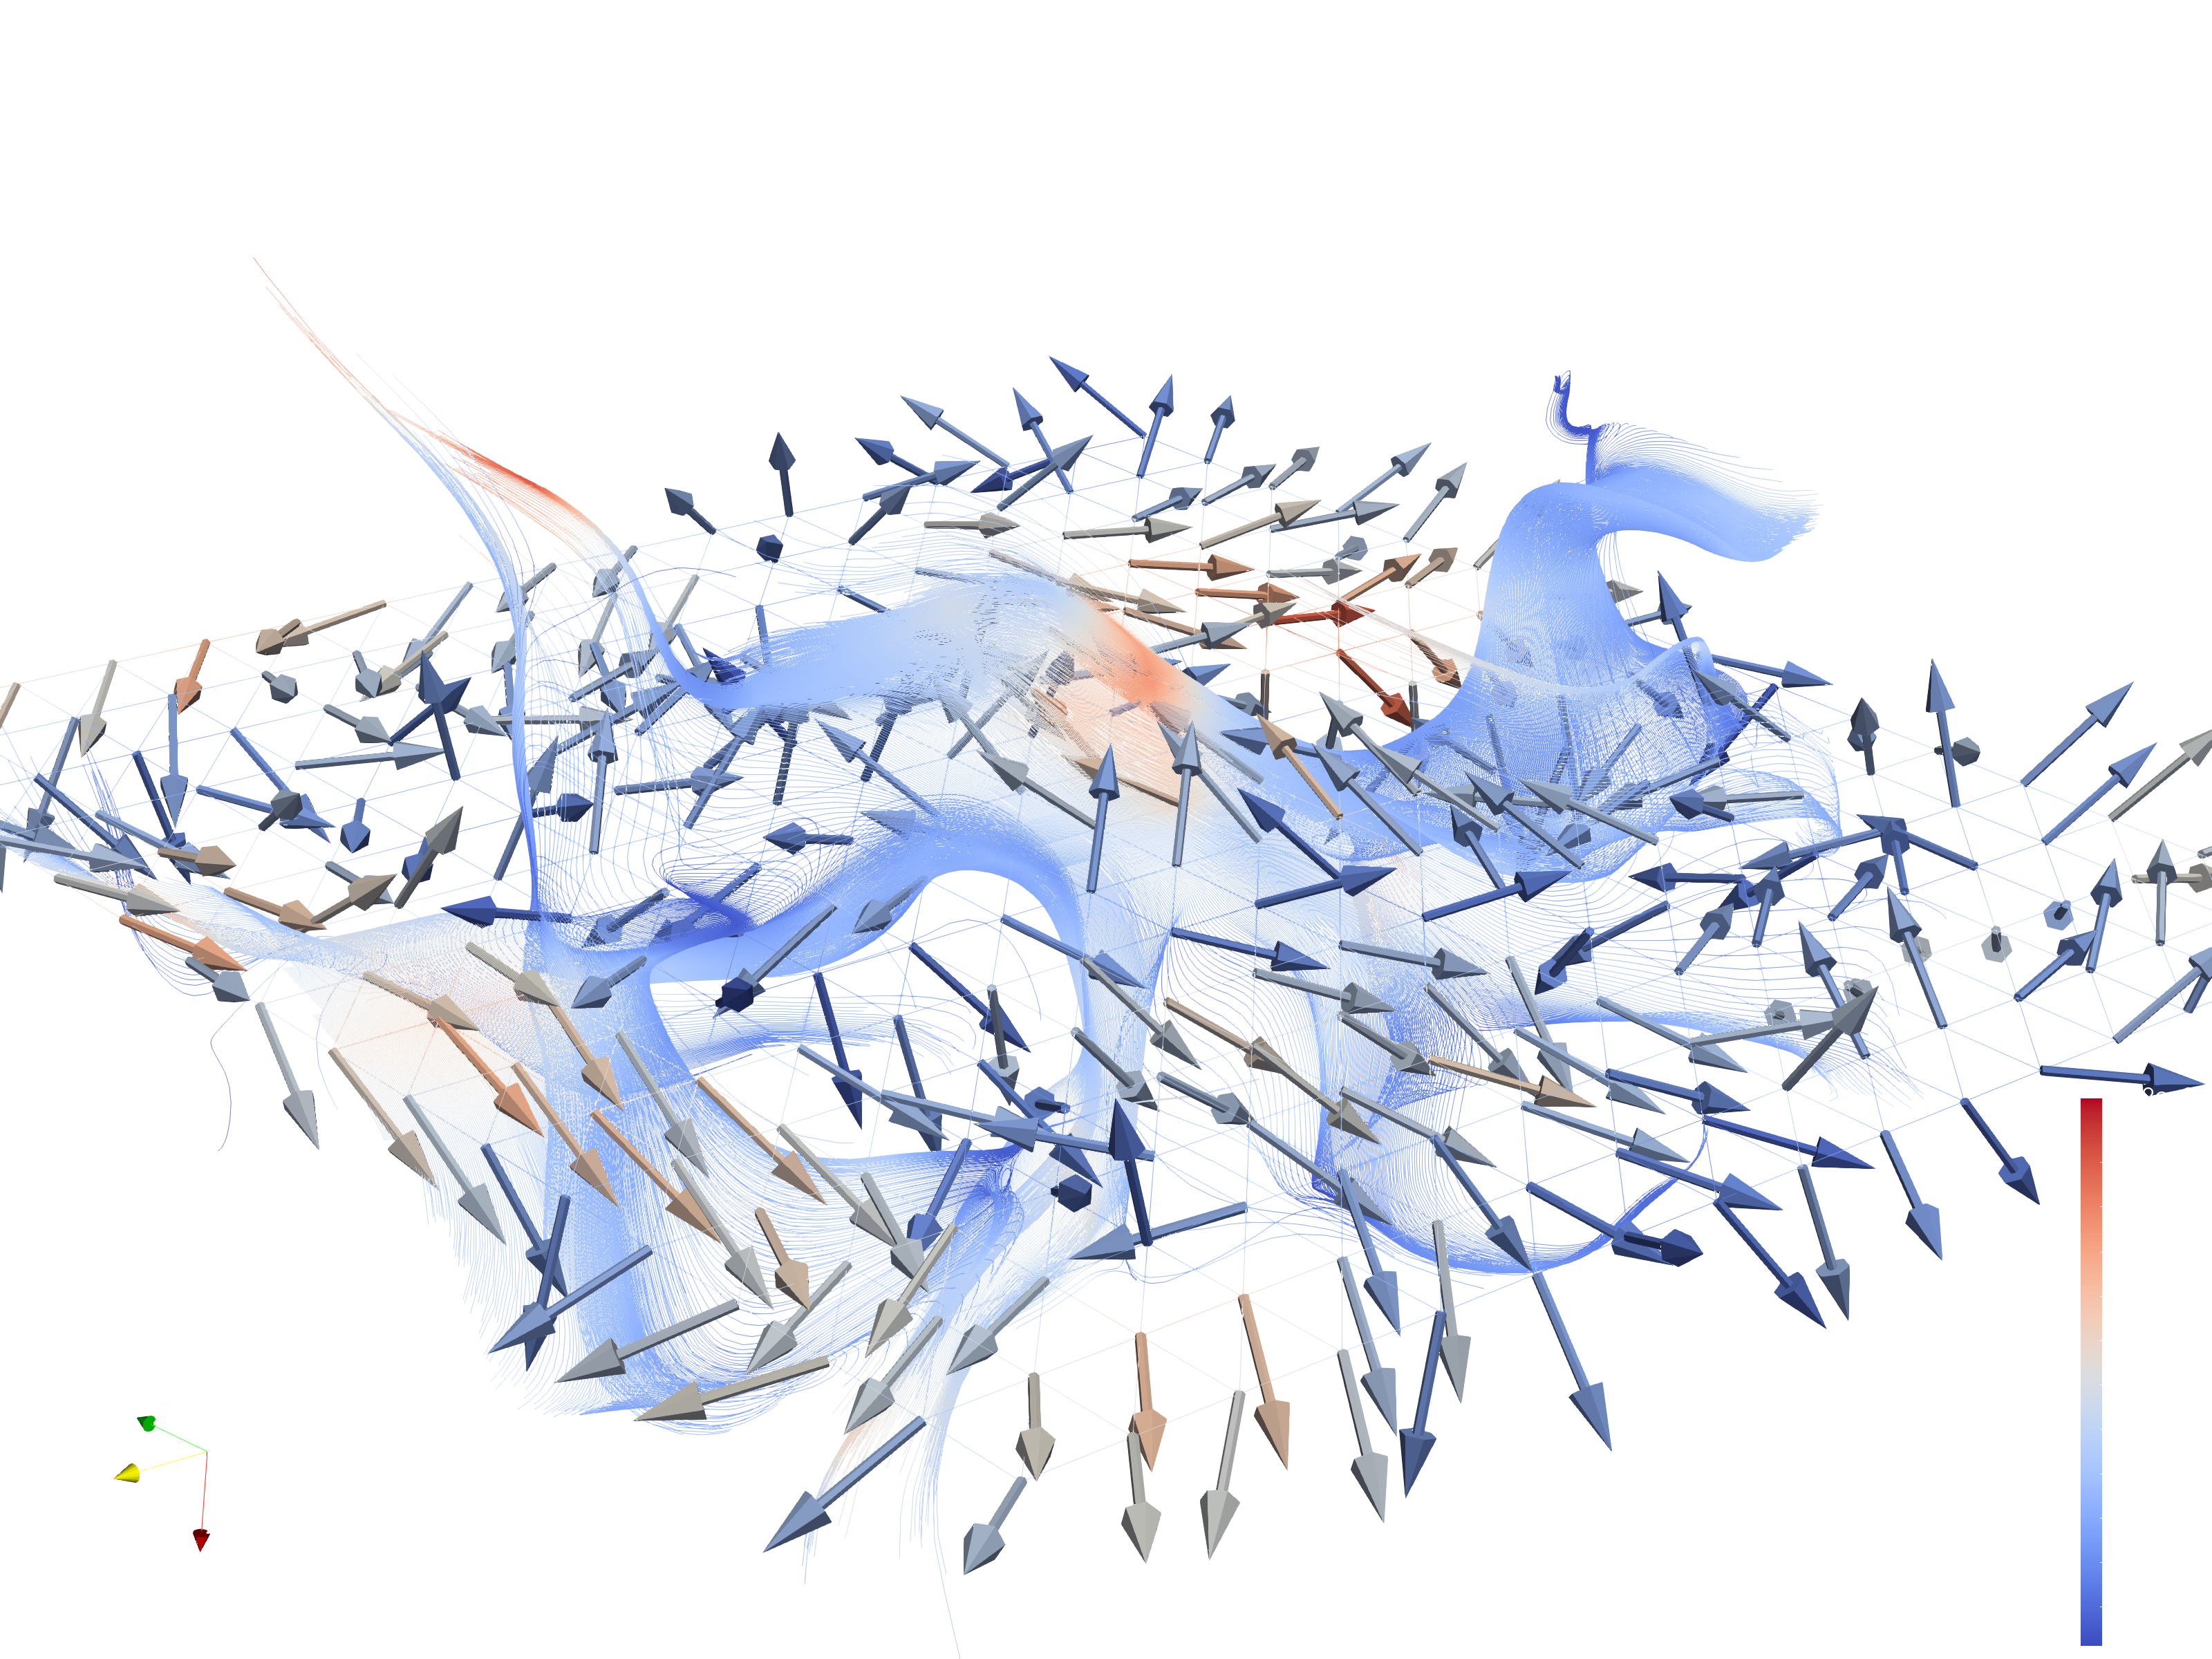
\includegraphics[width=0.4\linewidth]{images/kriging/3components/z_normal_xyplane_on_angle_with_stream_trace.png}} \\
        \hfill
        \subcaptionbox[List-of-Figures entry]{плоскость $xy$, $z = 0$\label{img:slice_velcotiy_field_xy_znormal_angle_2}} 
        {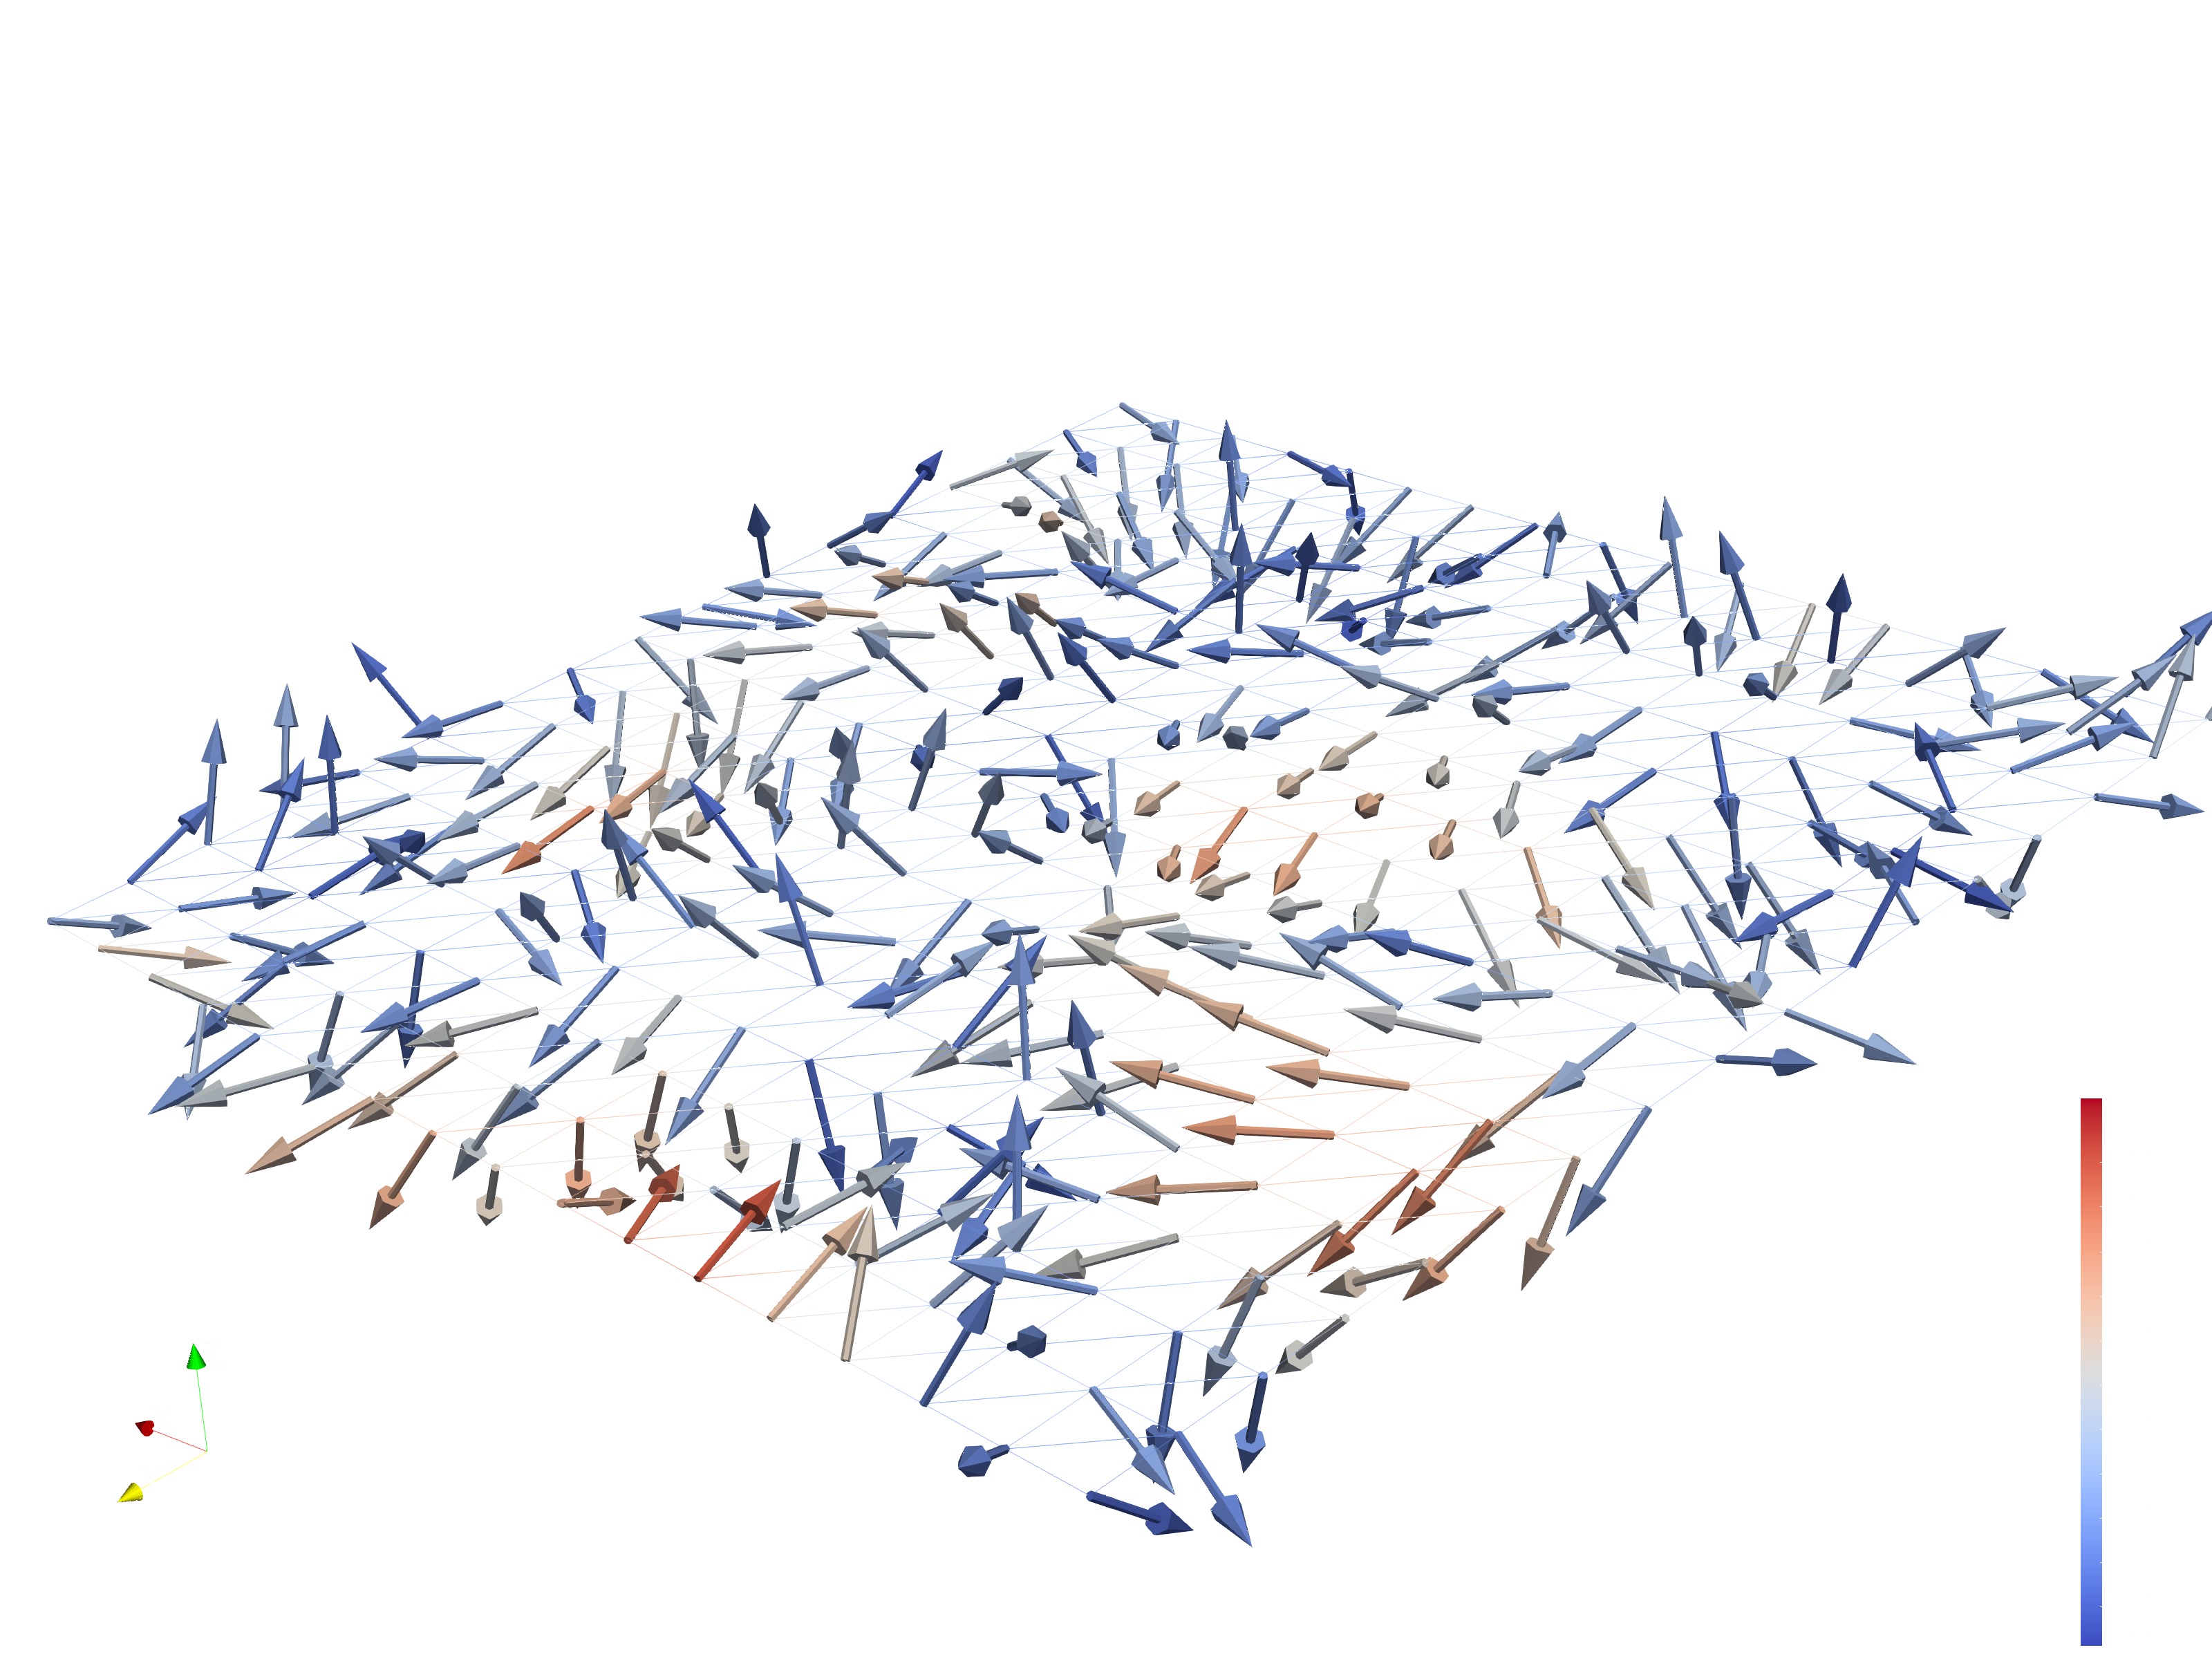
\includegraphics[width=0.4\linewidth]{images/kriging/3components/z_normal_xyplane_on_angle.png}}%
        \hfill       
        \subcaptionbox{плоскость $xy$, $z = 0$\label{img:slice_velcotiy_field_xy_znormal_no_angle}} 
        {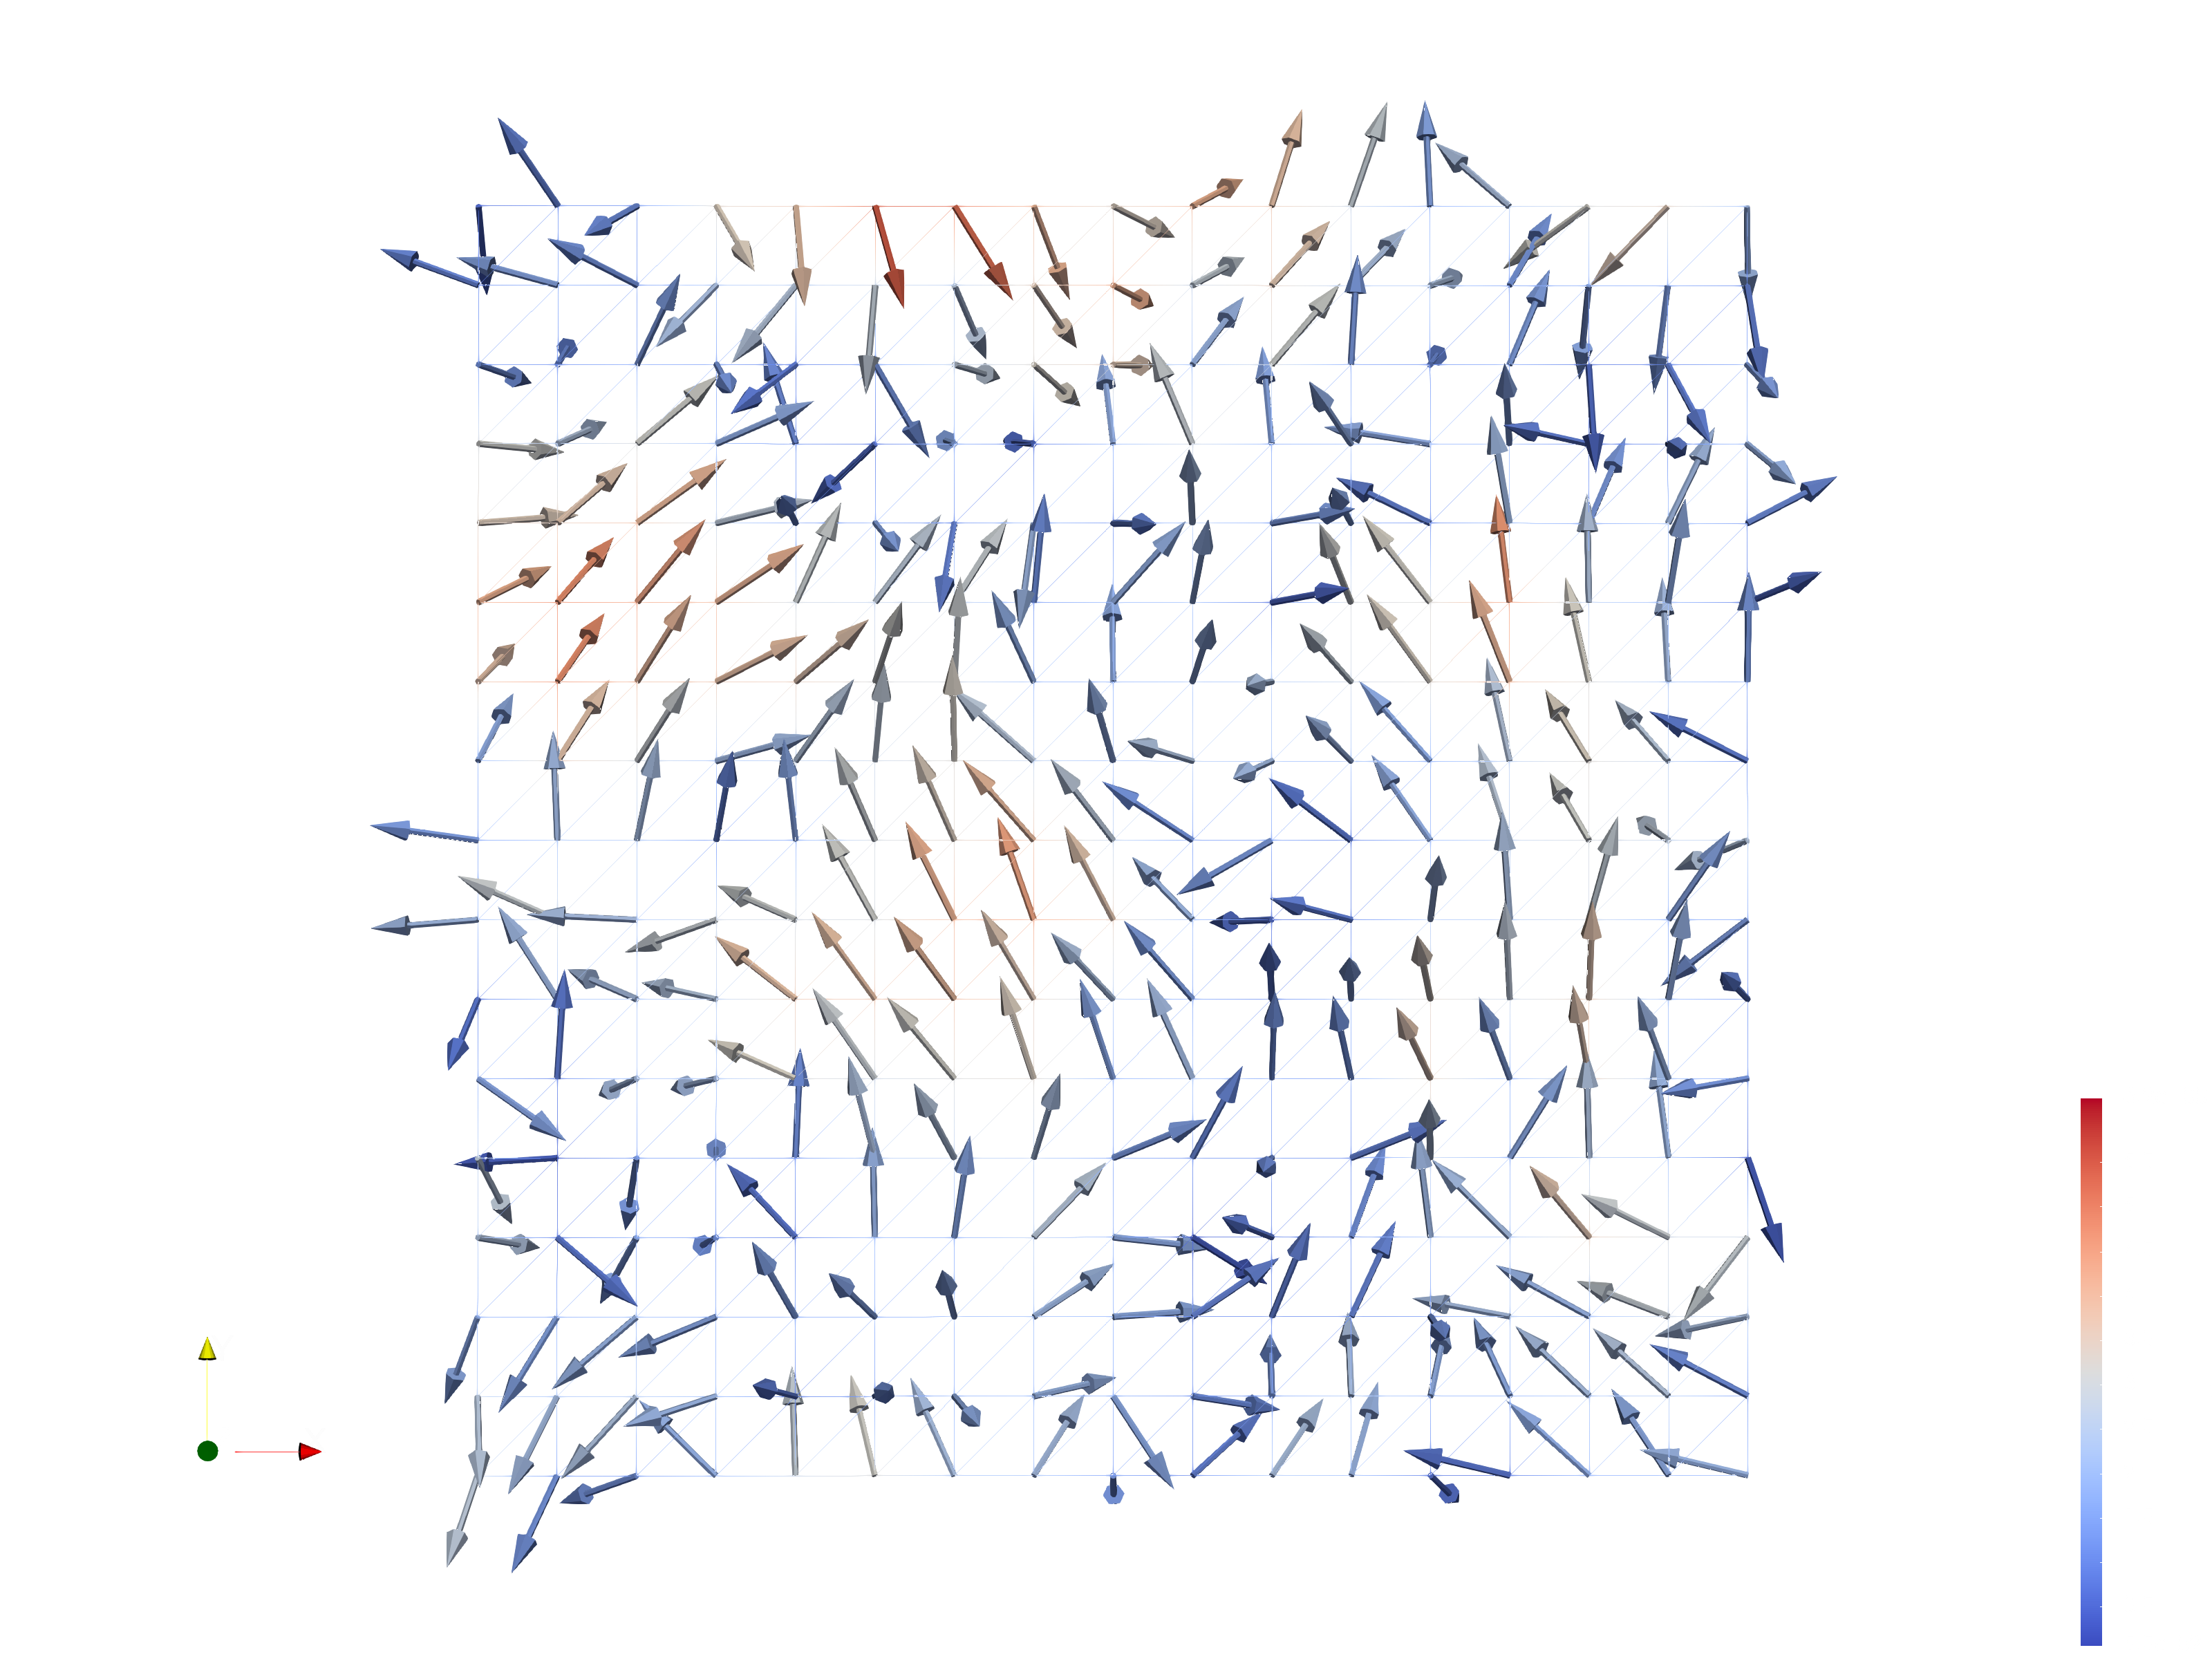
\includegraphics[width=0.4\linewidth]{images/kriging/3components/z_normal_xyplane.png}}
        \hfill
    }
    
    \onehalfspacing{Поле на картинке б представлено с линиями тока, расчитанными вдоль оси $y$}
    \caption{Поле флуктуаций сгенерированных трёхмерным стохастическим методом, цветом обозначена амплитуда флуктуаций}
    \label{img:velocity_fluctuation_field_forkriging}  
\end{figure}

Приведём тепловые карты тензора ковариаций полученного из целевого спектра при помощи \eqref{eq:part3_2} и \eqref{eq:kriging_equation14_2}.

%
% Точная ковариация
%
\begin{figure}[!h]
    \center{
        \hfill
        \subcaptionbox[List-of-Figures entry]{$R_{xx}$  $x$-нормаль\label{img:kriging_exact_cov_r_11}} 
        {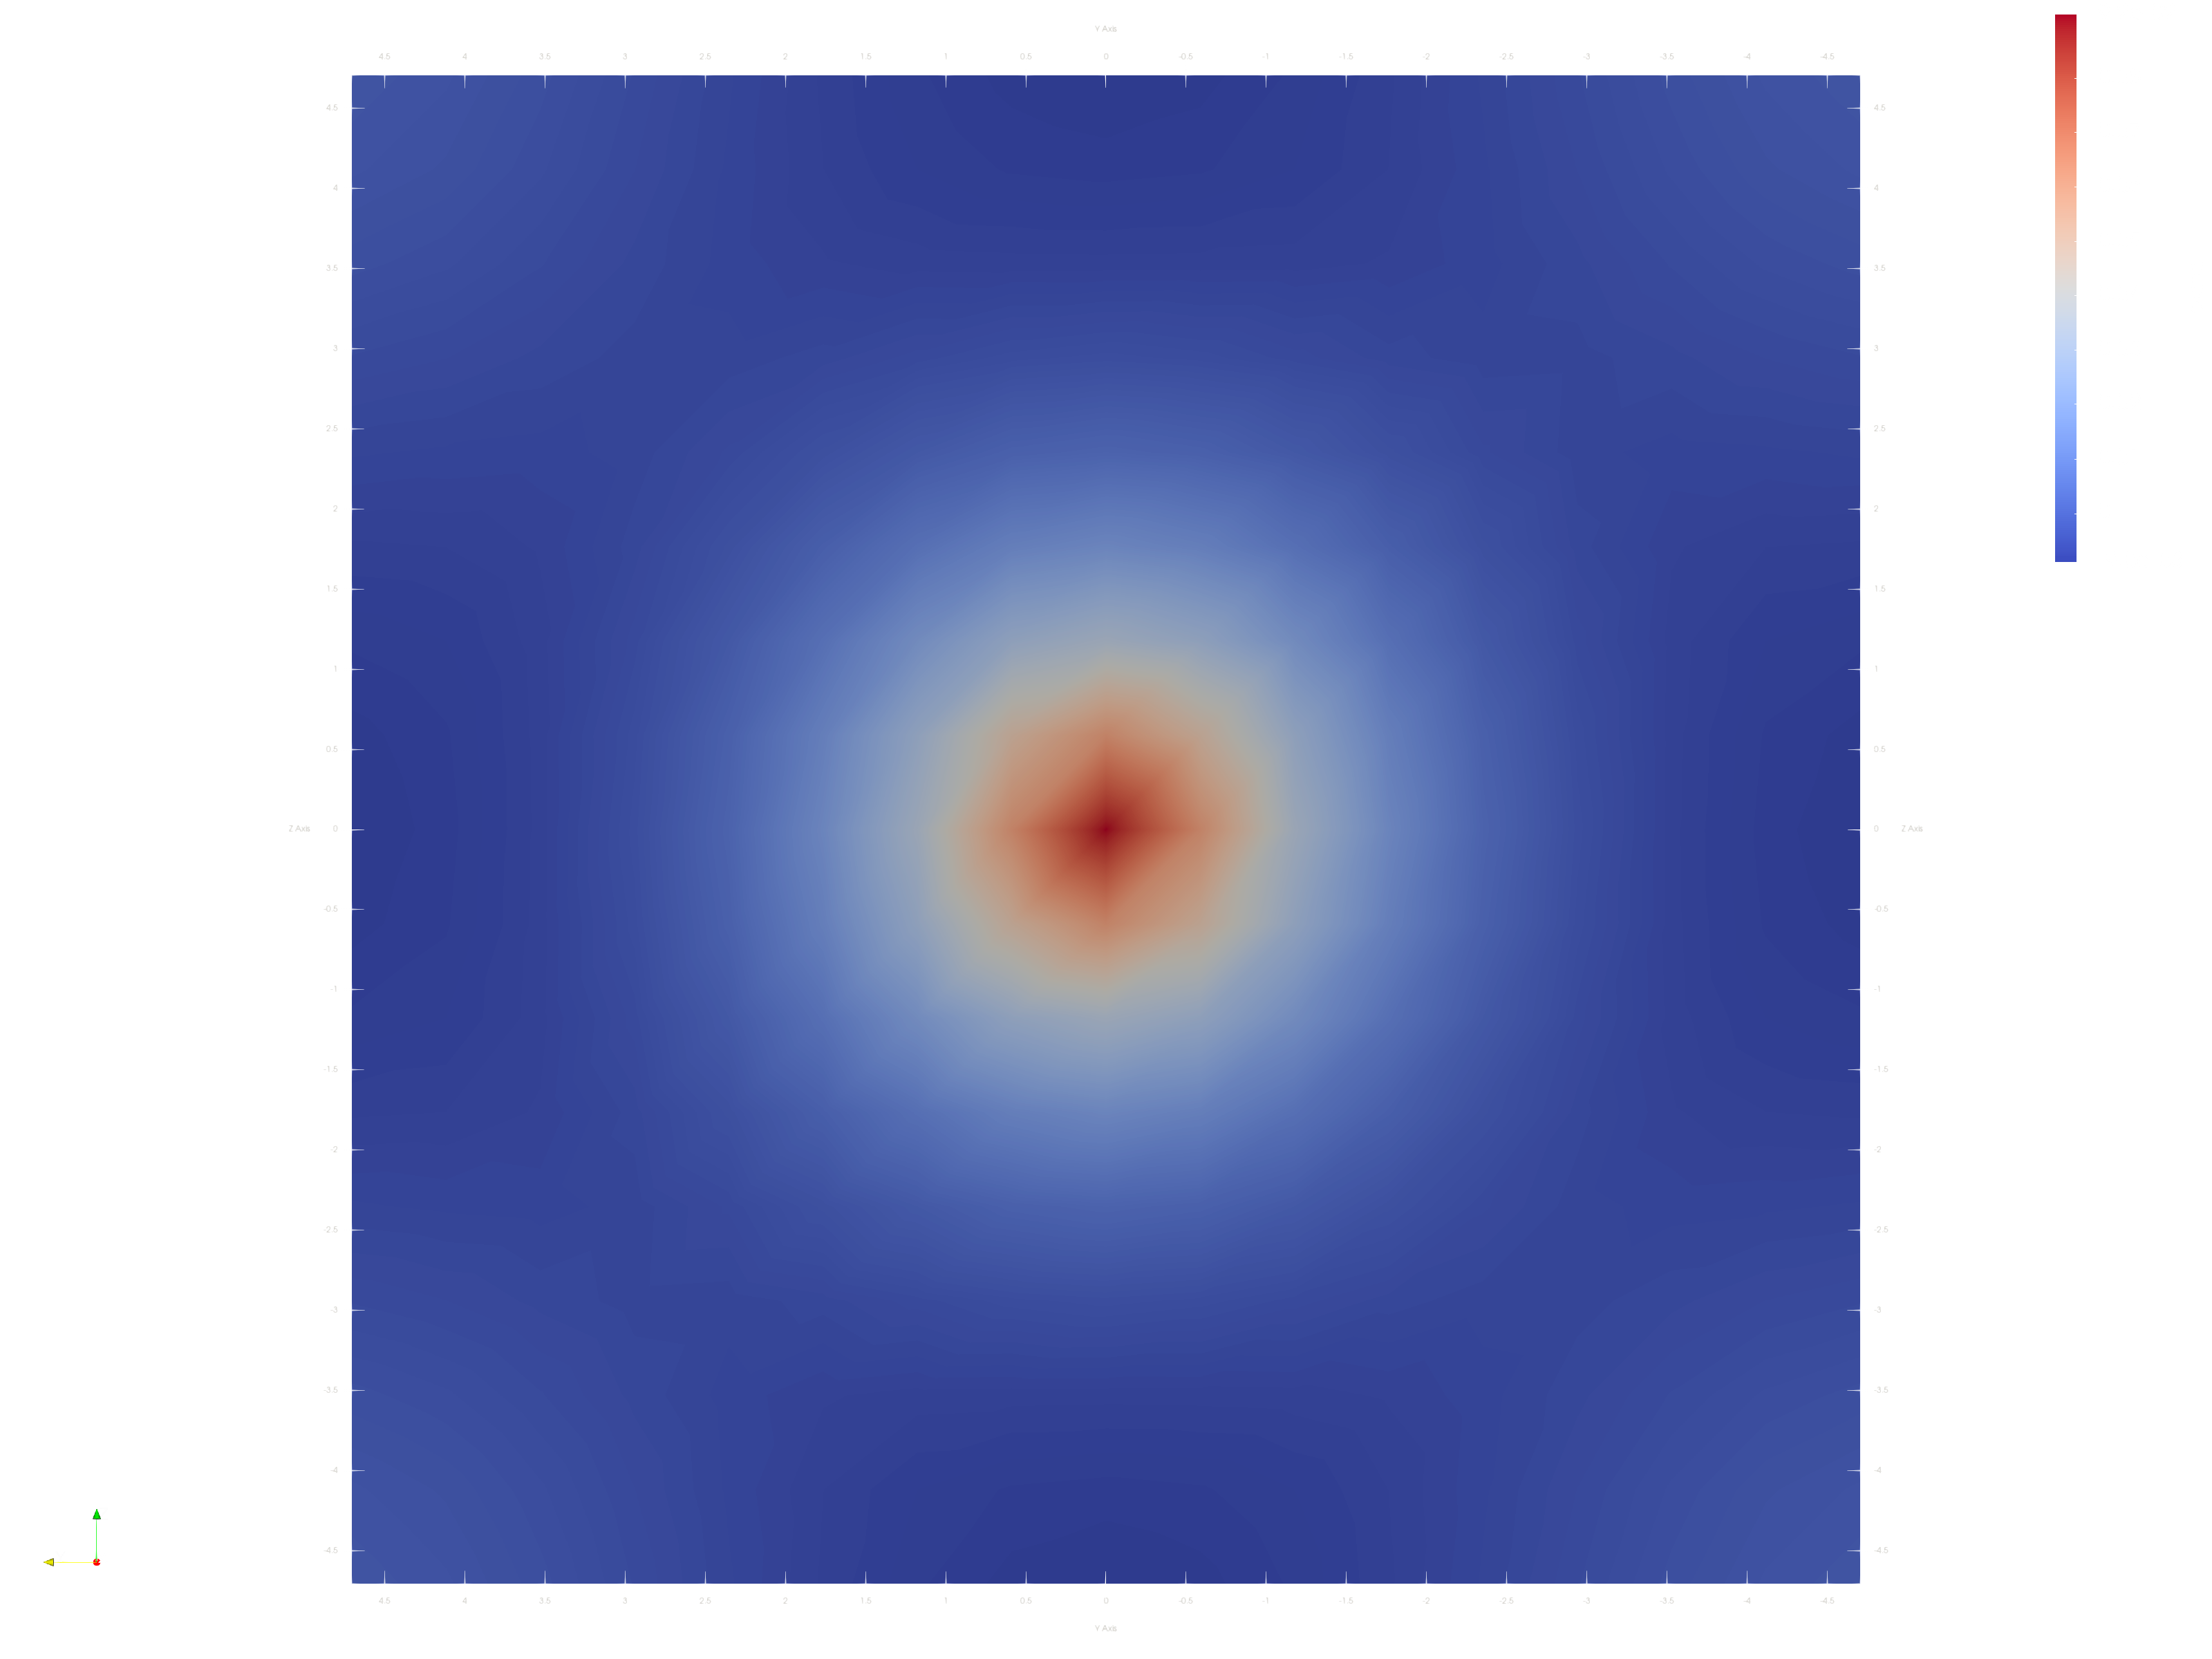
\includegraphics[width=0.32\linewidth]{images/kriging/3components/exact_cov_11_xx.png}}%
        \hfill       
        \subcaptionbox{$R_{xx}$  $y$-нормаль \label{img:kriging_exact_cov_r_12}} 
        {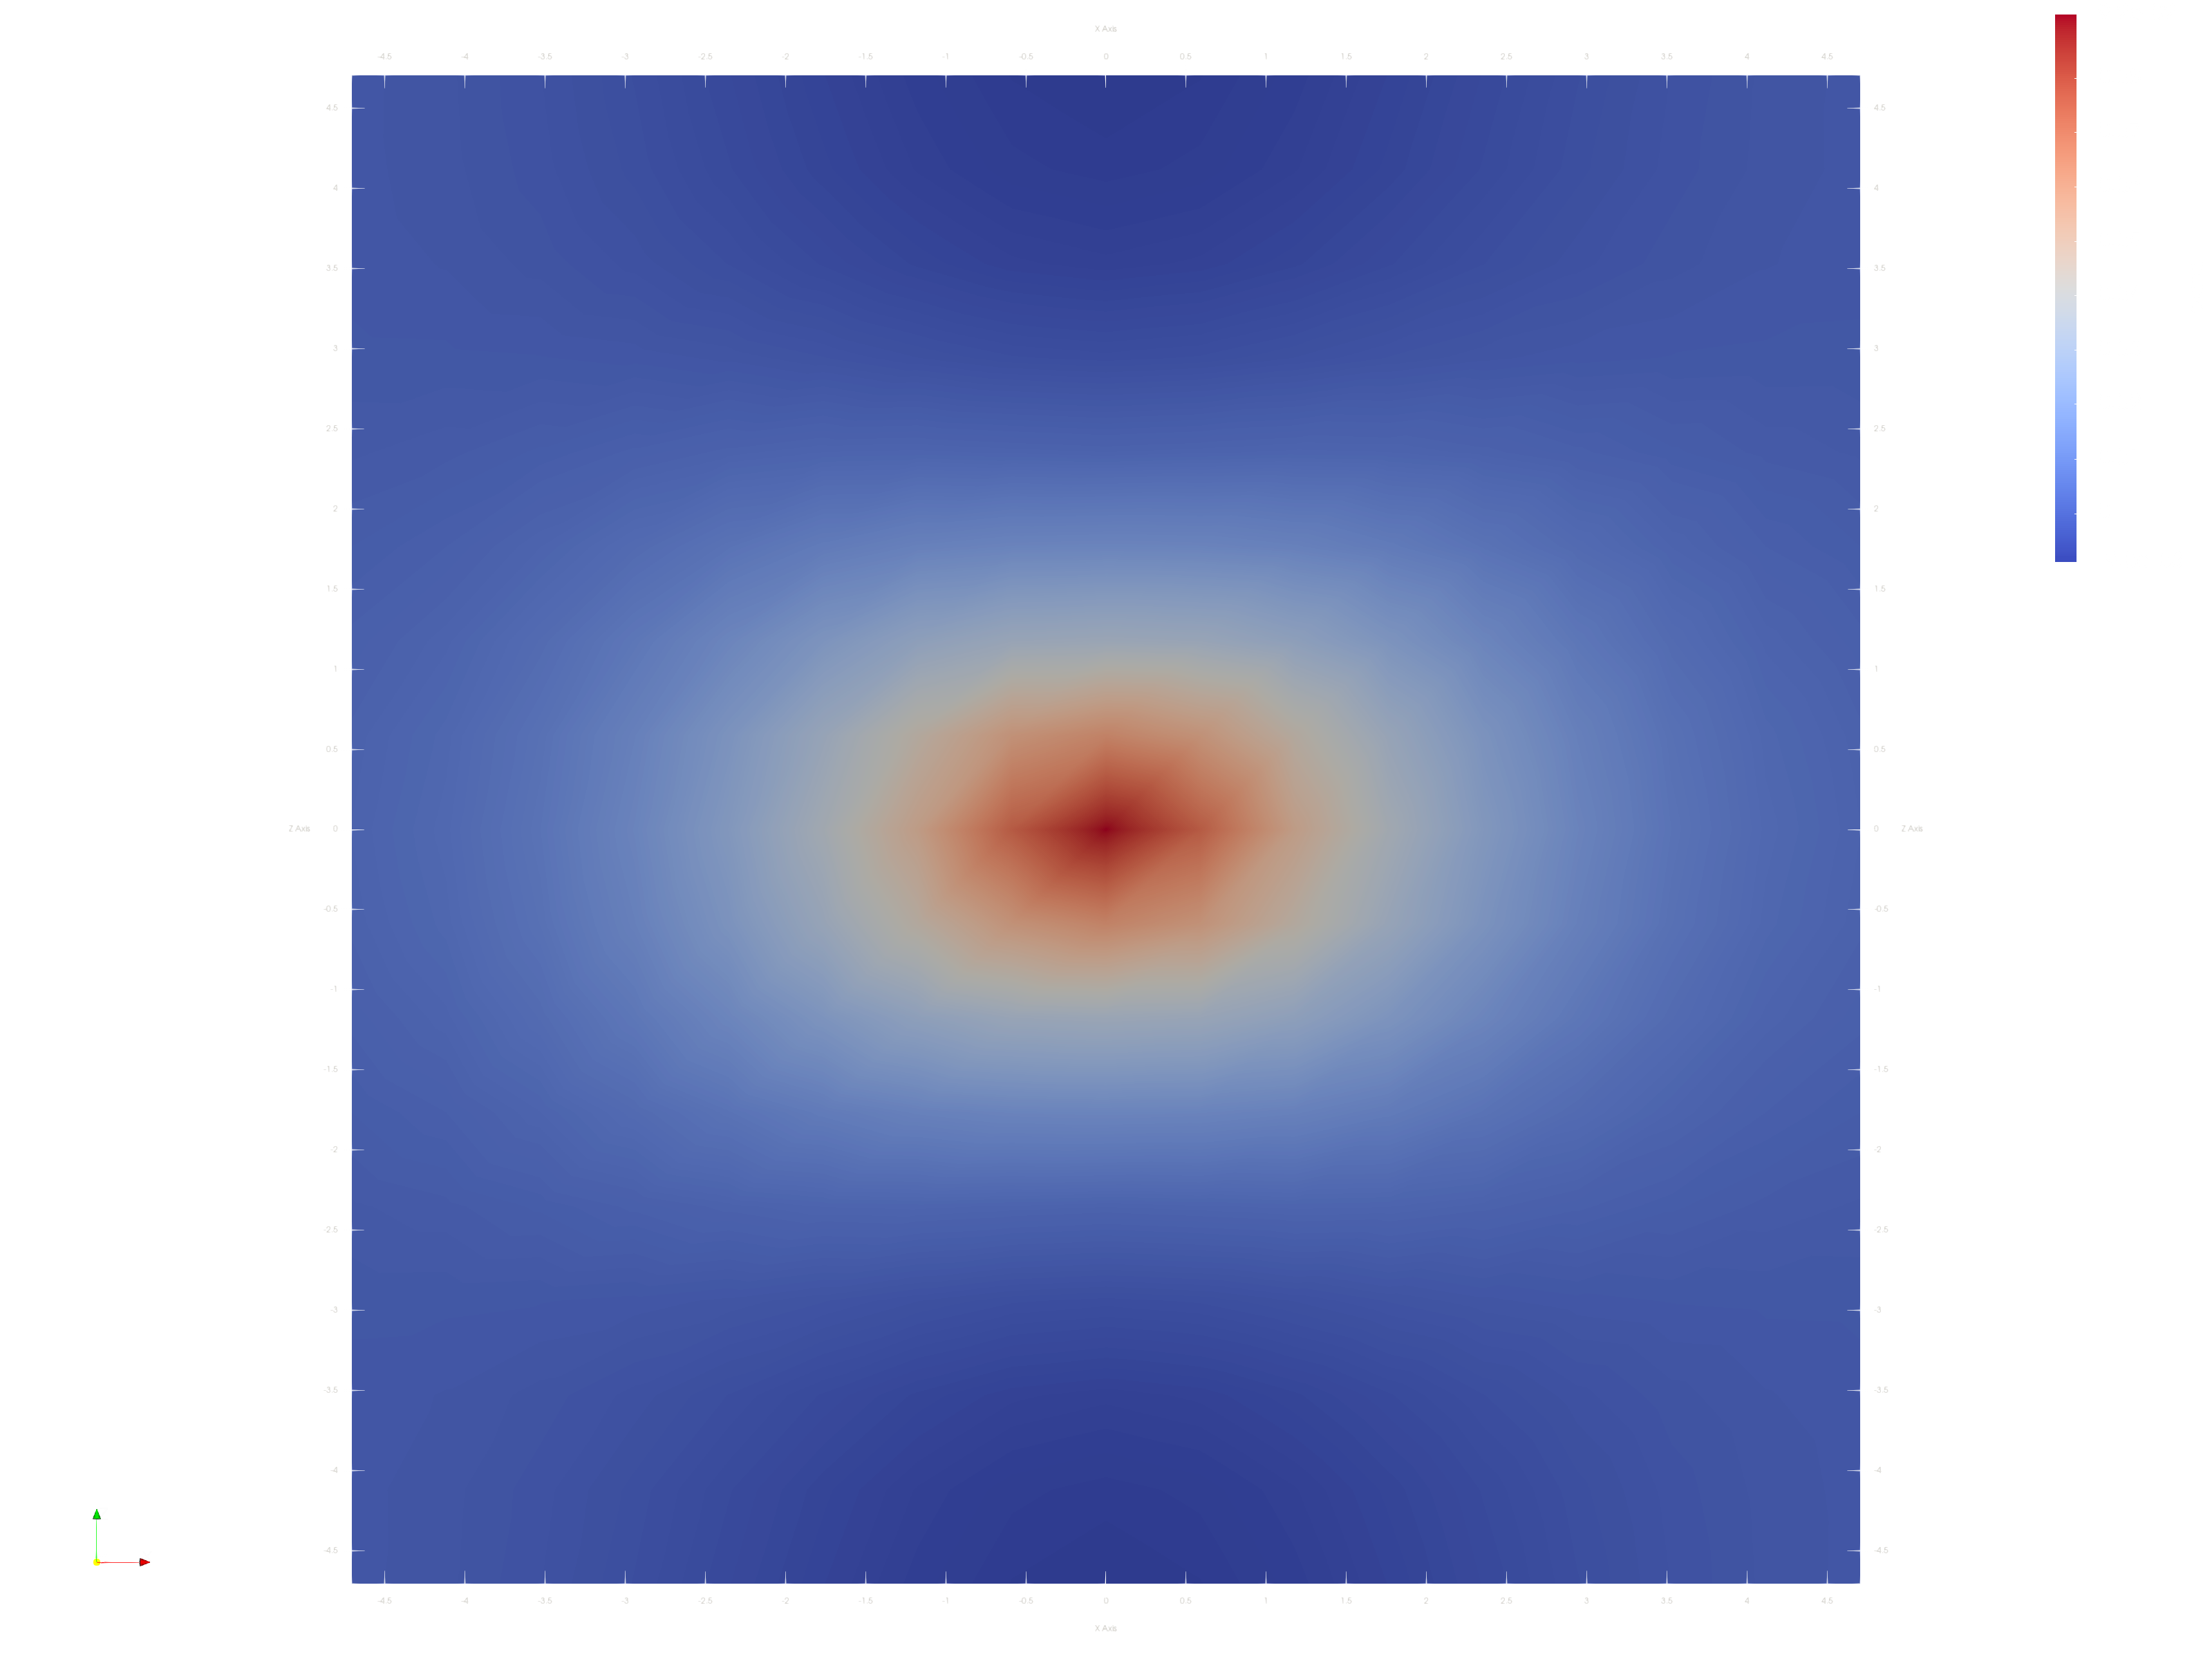
\includegraphics[width=0.32\linewidth]{images/kriging/3components/exact_cov_11_yy.png}}
        \hfill
        \subcaptionbox{$R_{xx}$  $z$-нормаль\label{img:kriging_exact_cov_r_13}} 
        {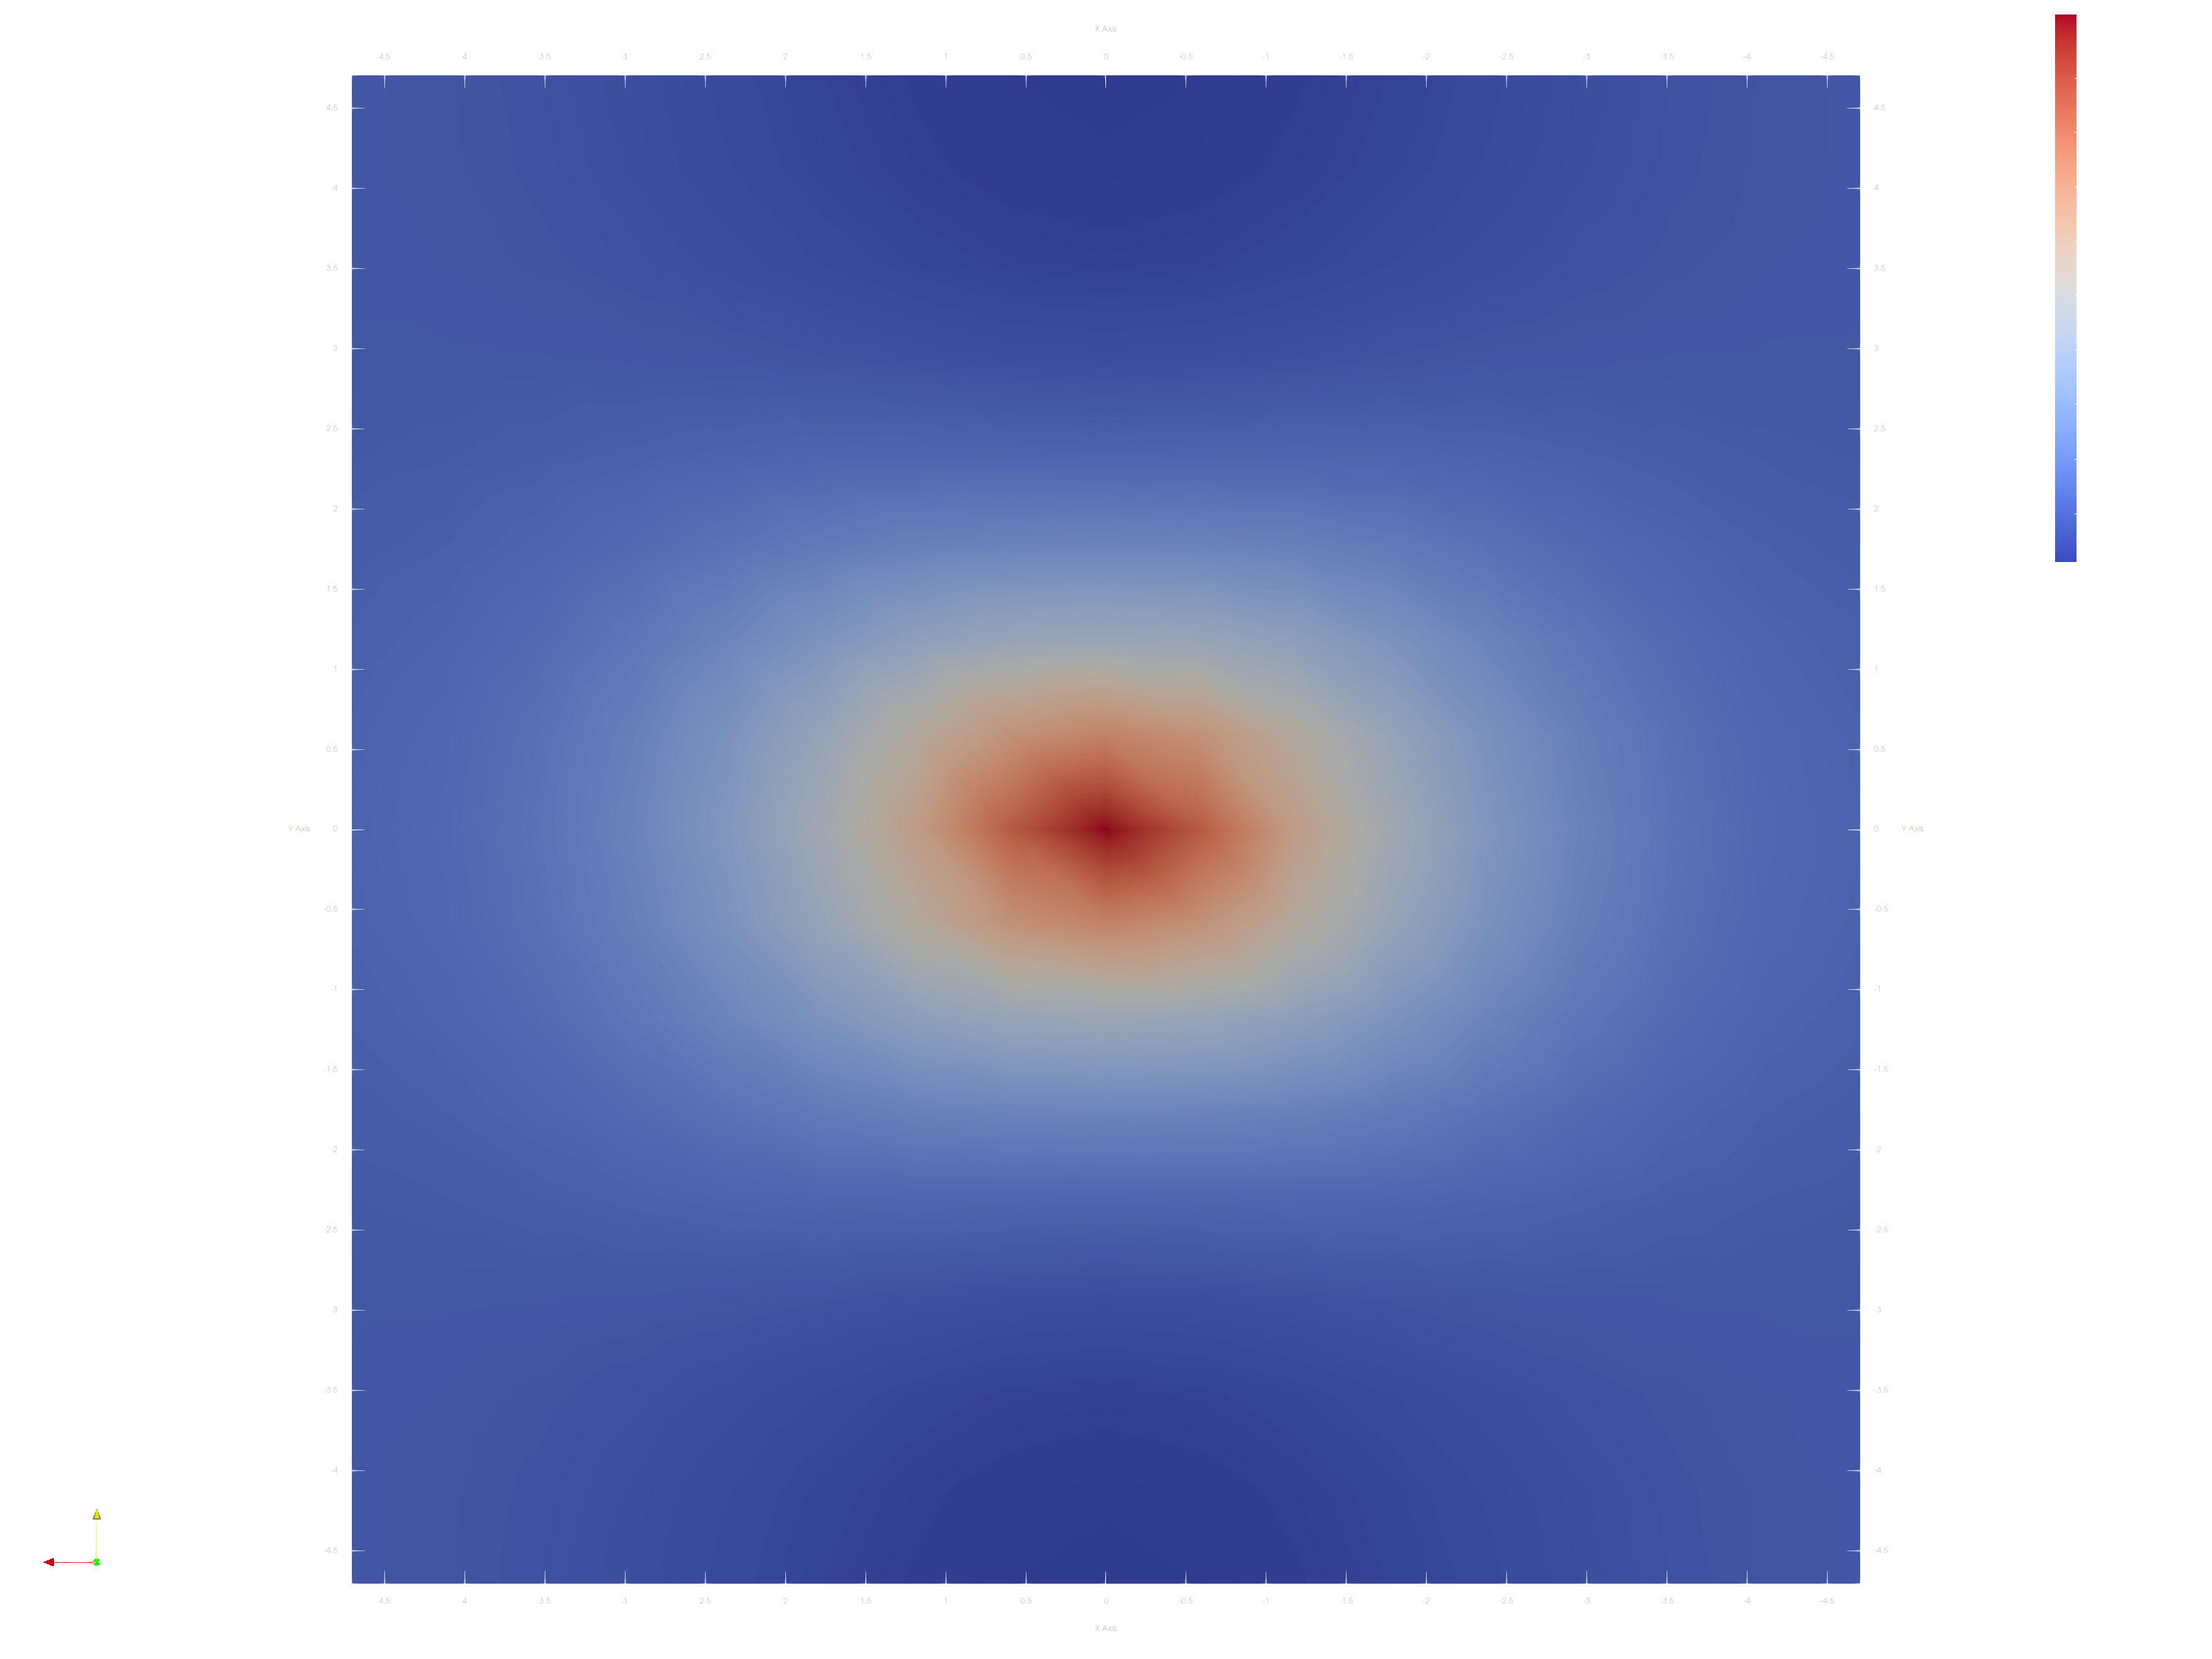
\includegraphics[width=0.32\linewidth]{images/kriging/3components/exact_cov_11_zz.png}}%
        \hfill       
        
        \subcaptionbox{$R_{yy}$ $x$-нормаль \label{img:kriging_exact_cov_r_22}} 
        {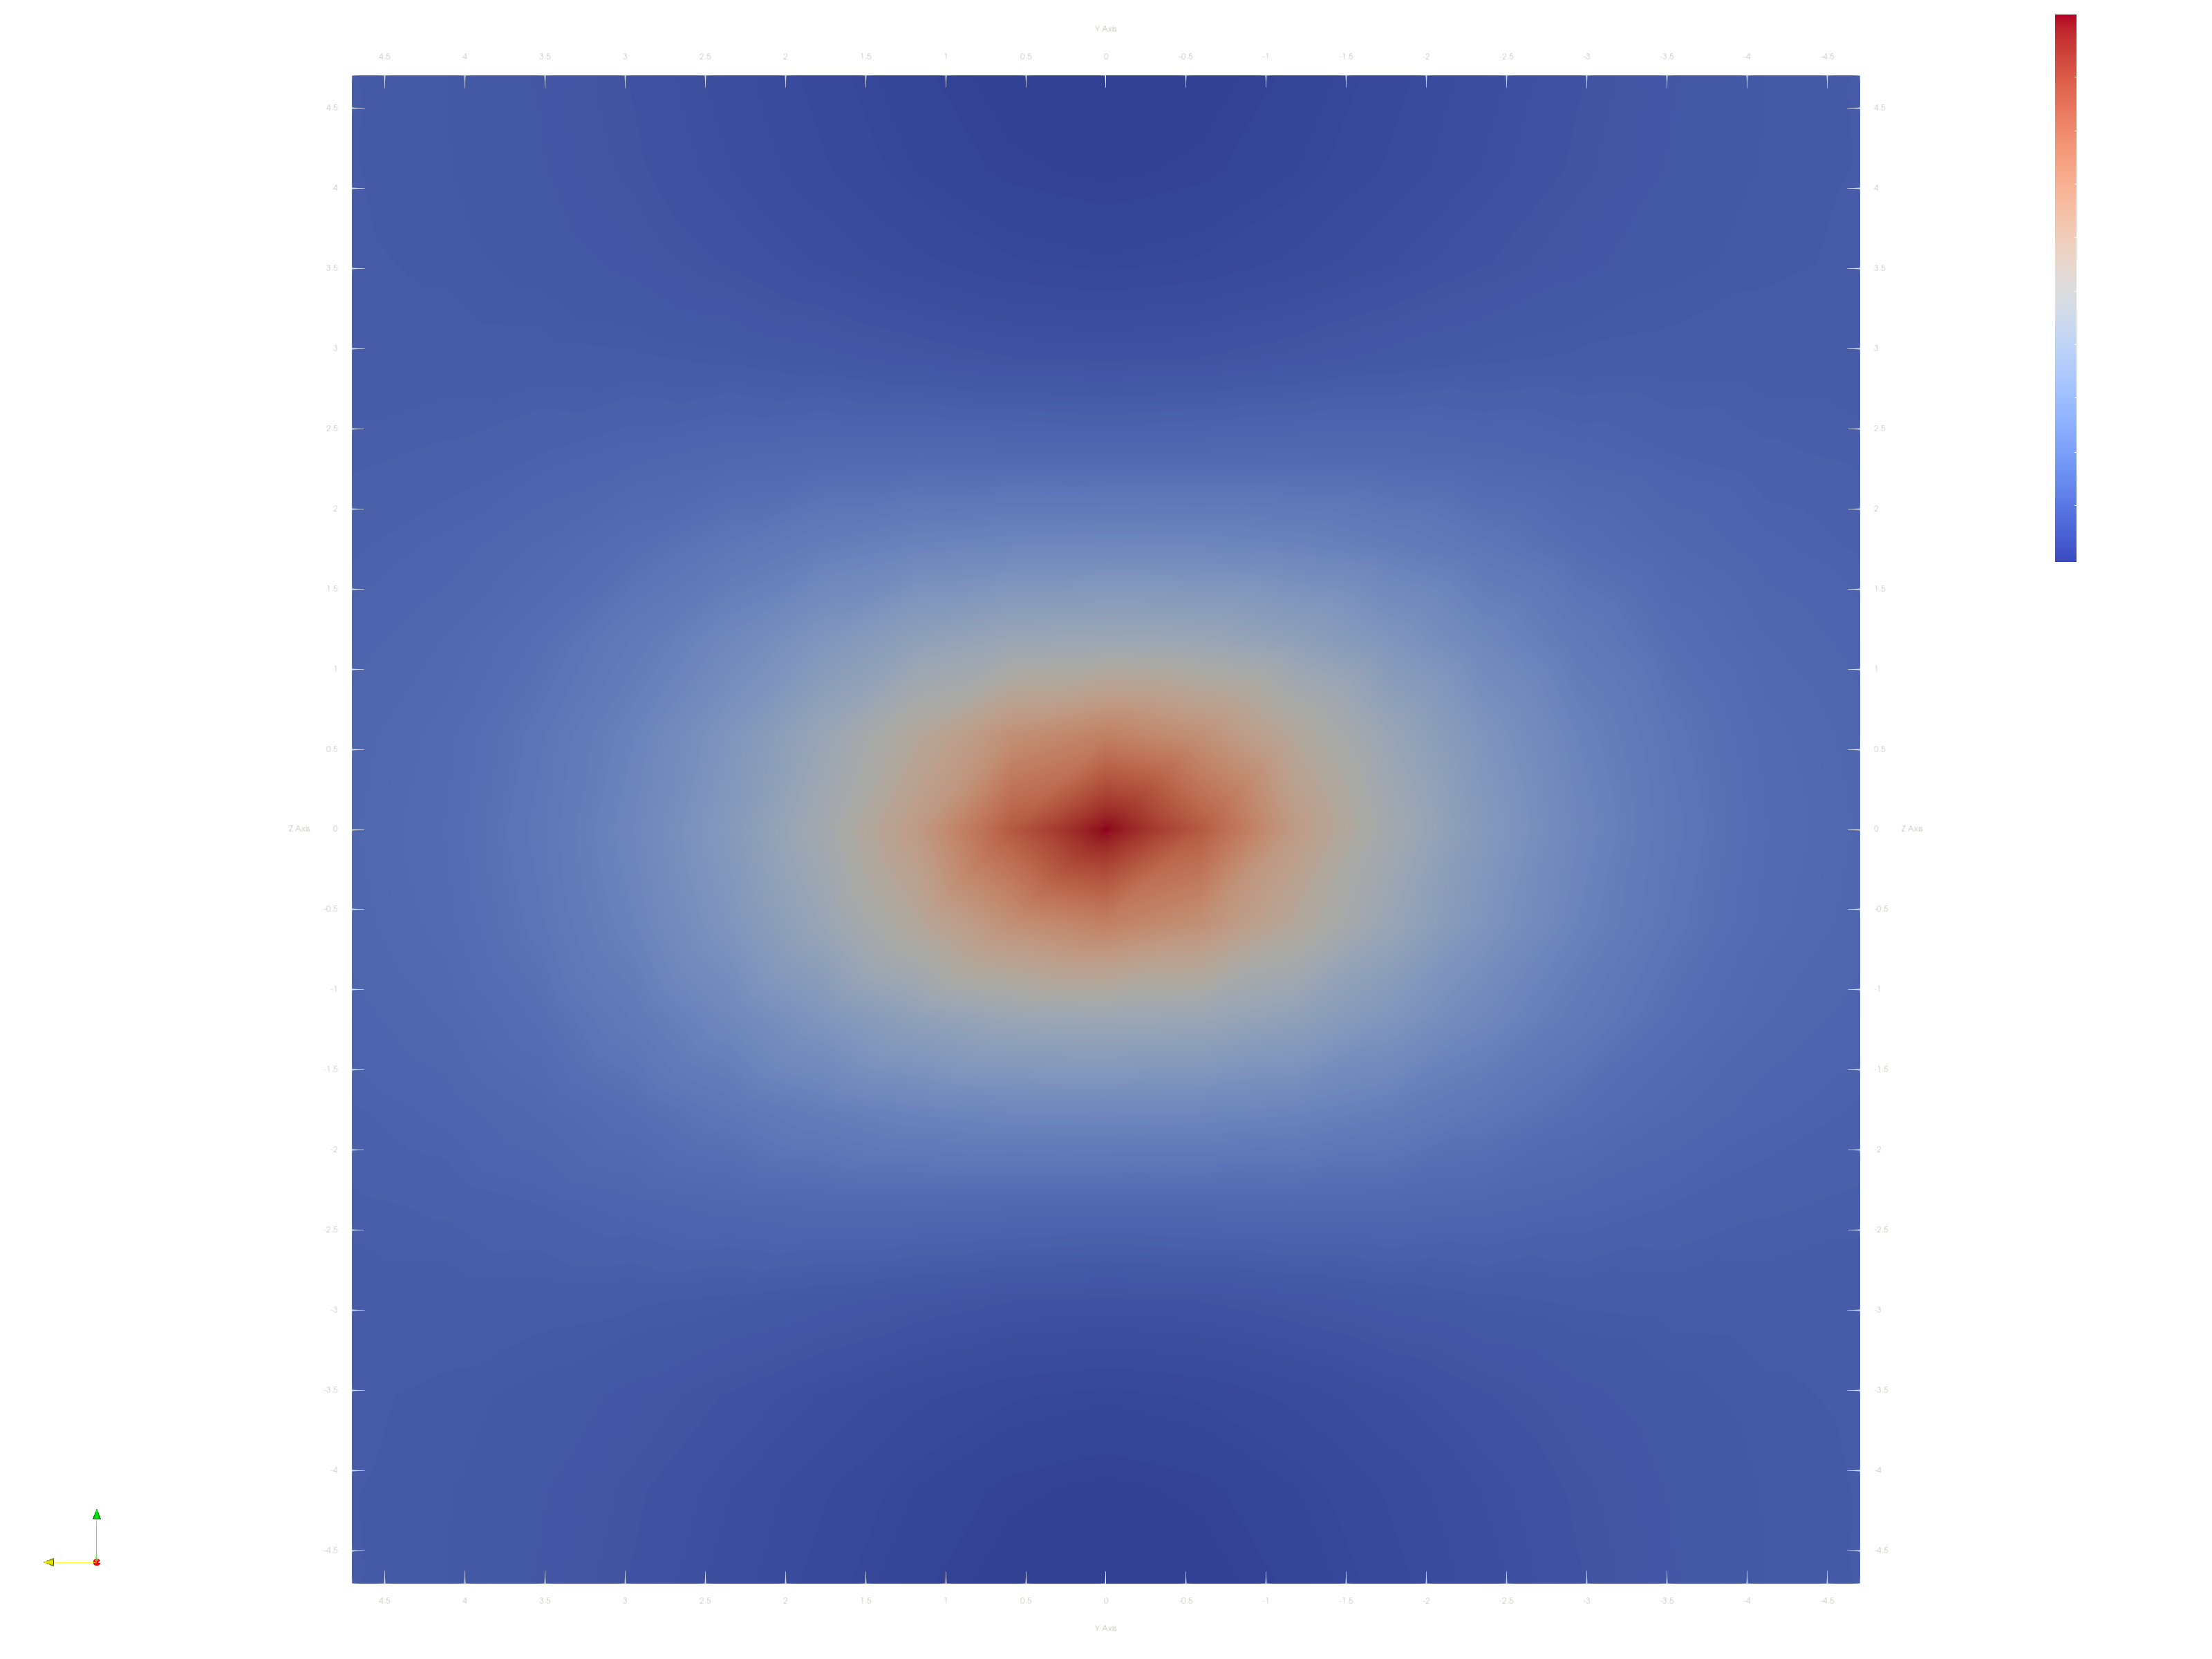
\includegraphics[width=0.32\linewidth]{images/kriging/3components/exact_cov_22_xx.png}}
        \hfill
        \subcaptionbox{$R_{yy}$ $y$-нормаль \label{img:kriging_exact_cov_r_23}} 
        {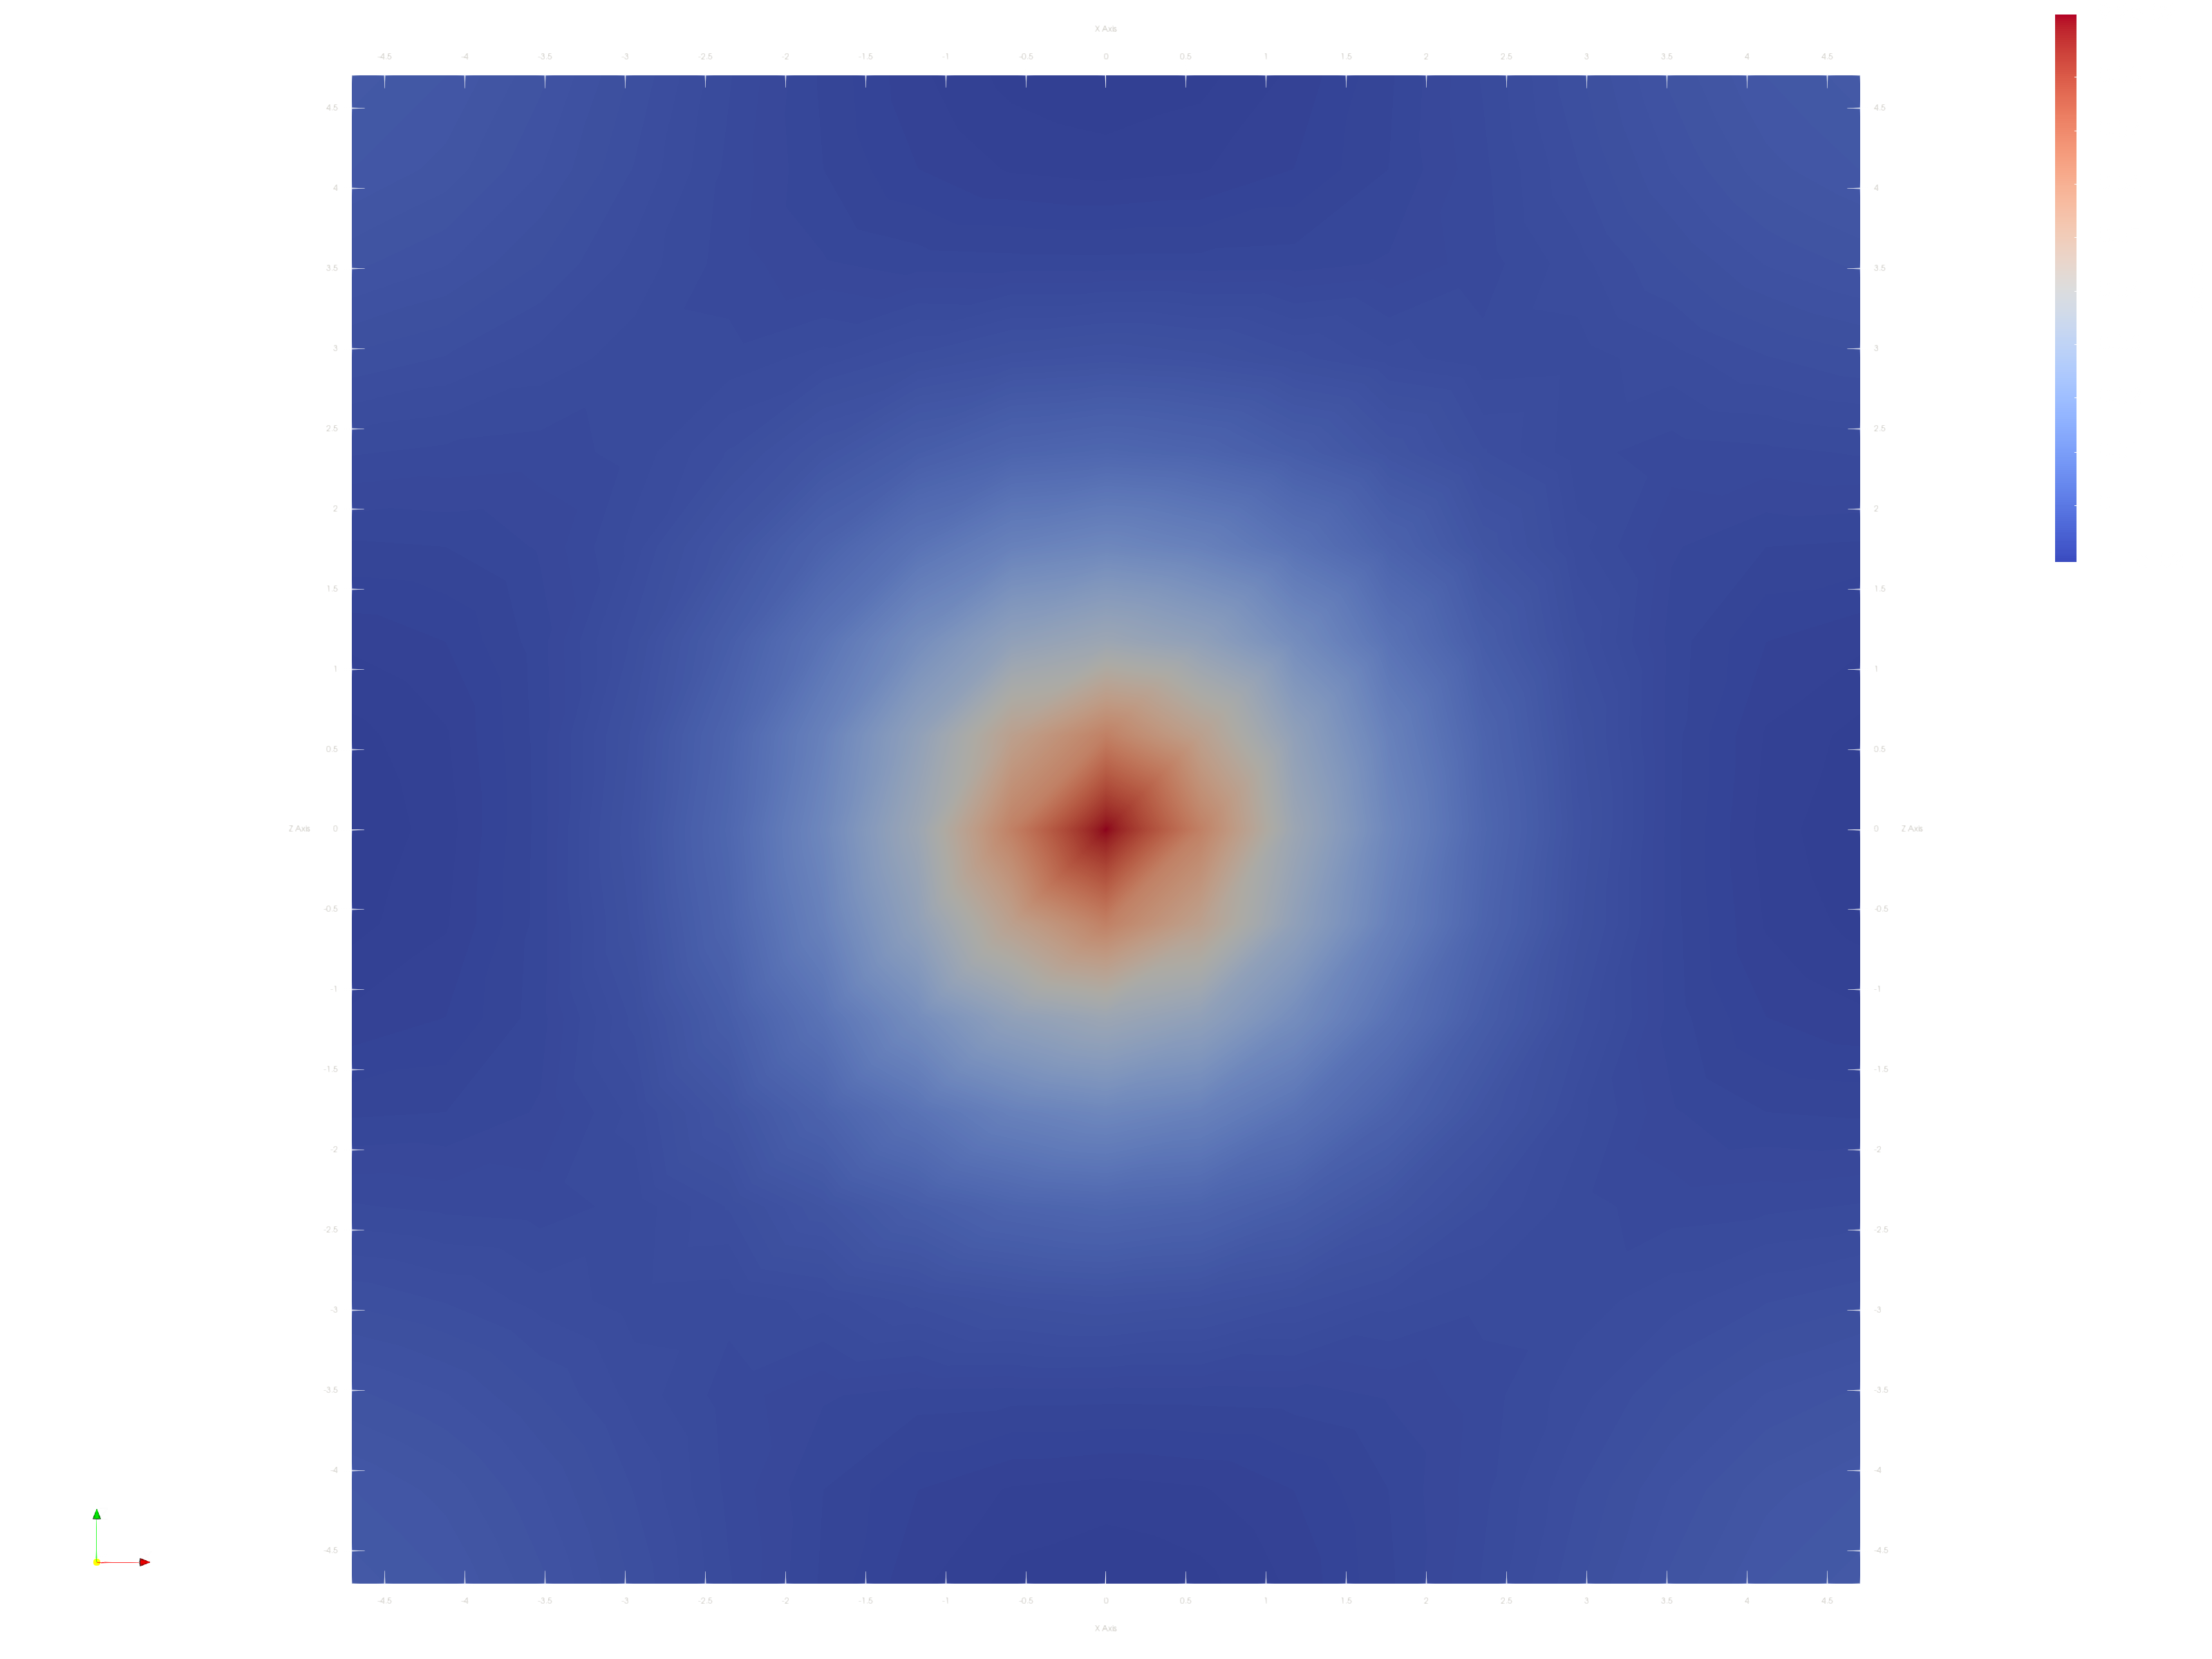
\includegraphics[width=0.32\linewidth]{images/kriging/3components/exact_cov_22_yy.png}}
        \hfill
        \subcaptionbox{$R_{yy}$ $z$-нормаль \label{img:kriging_exact_cov_r_33}} 
        {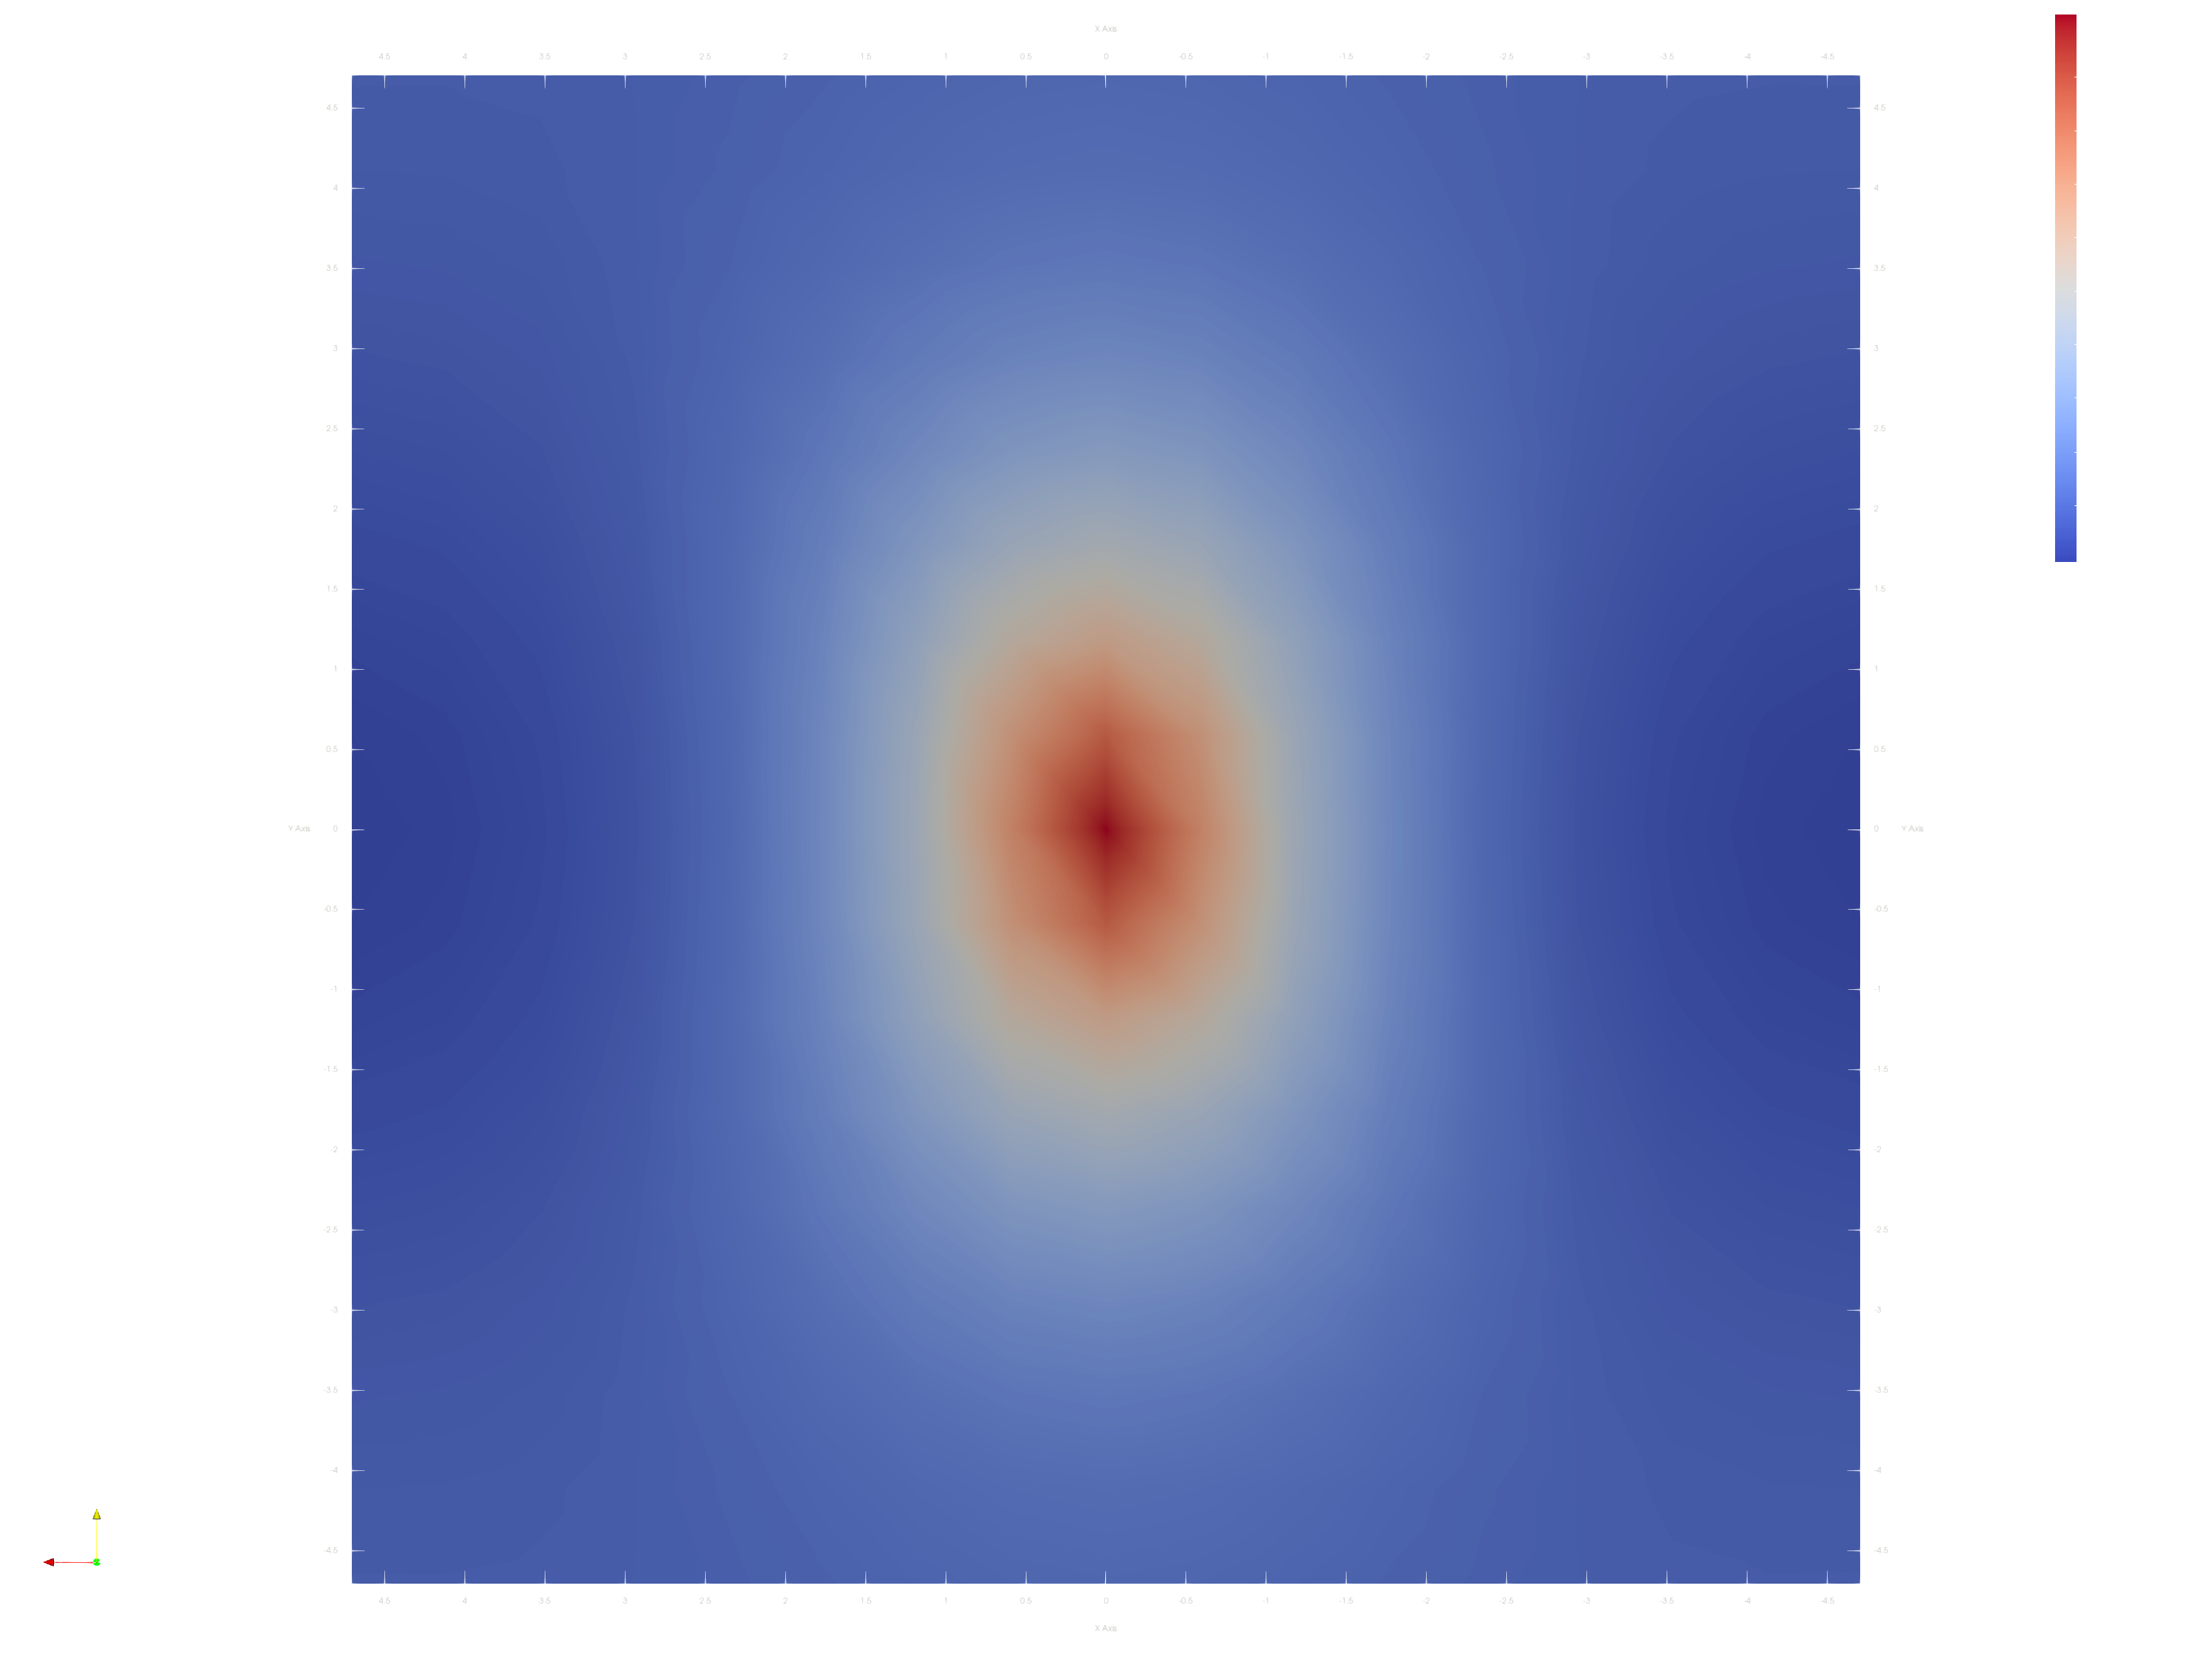
\includegraphics[width=0.32\linewidth]{images/kriging/3components/exact_cov_22_zz.png}}
        \hfill
        
        \subcaptionbox{$R_{zz}$ $x$-нормаль \label{img:kriging_exact_cov_r_22}} 
        {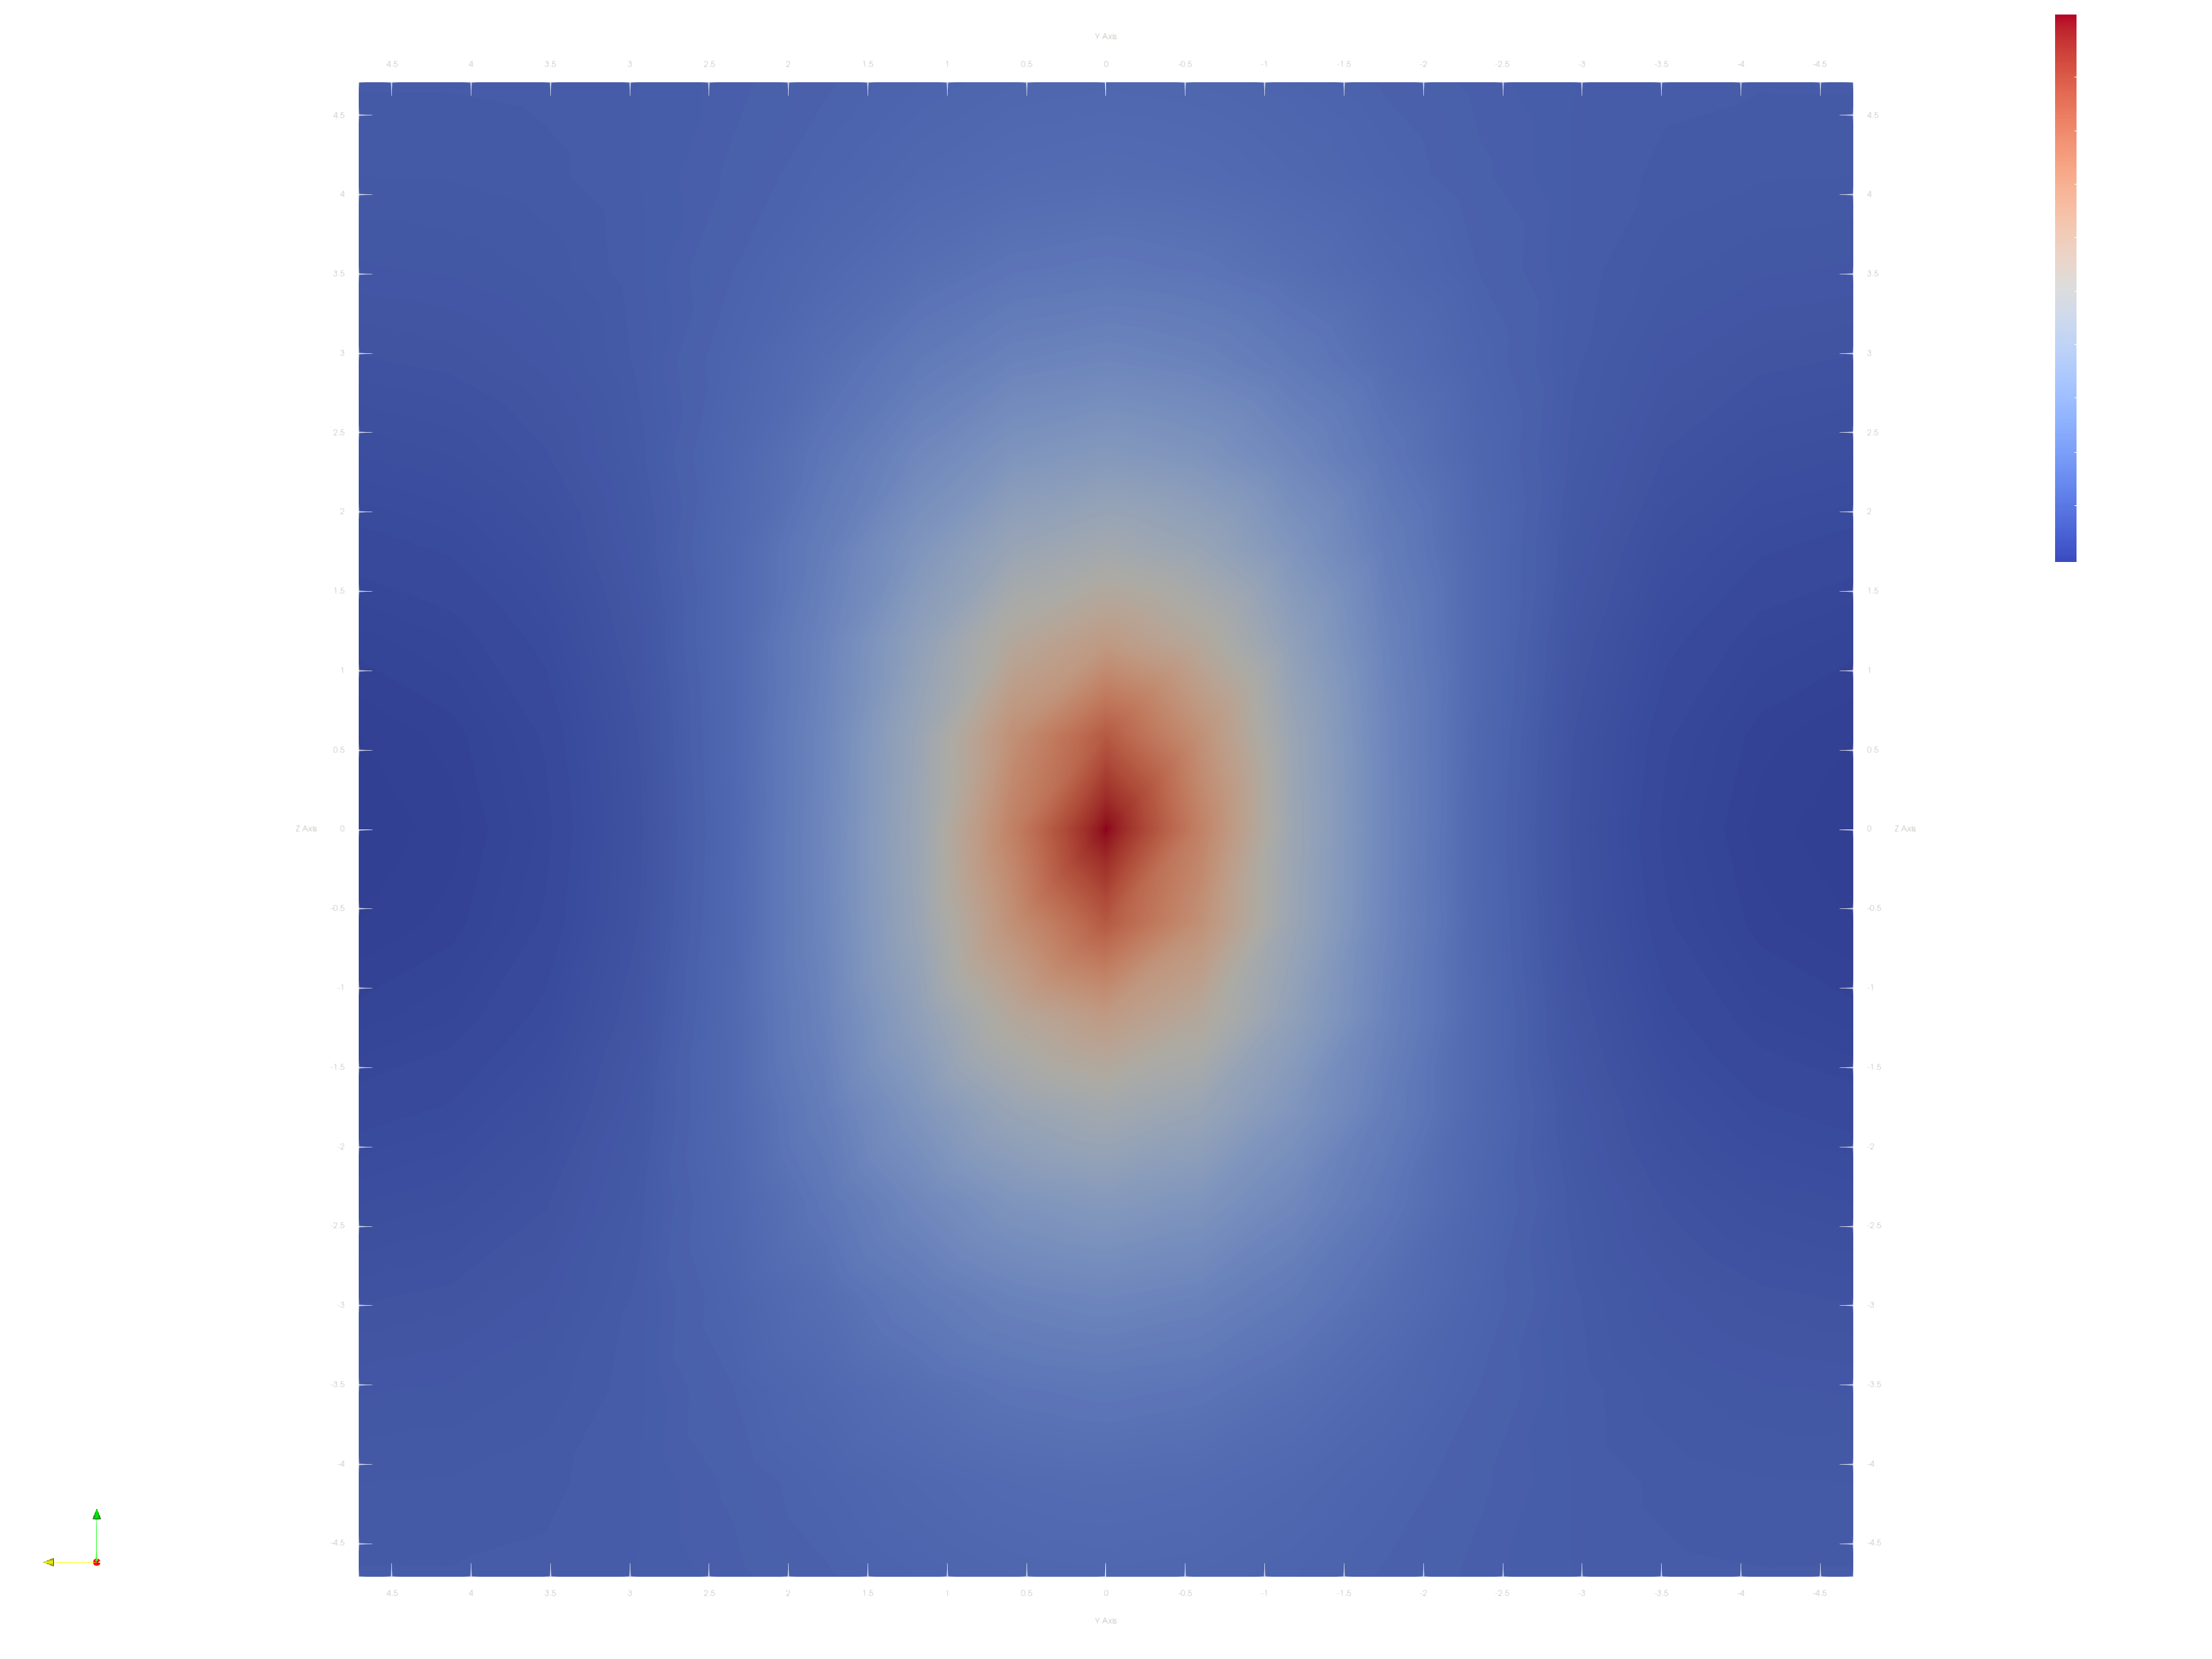
\includegraphics[width=0.32\linewidth]{images/kriging/3components/exact_cov_33_xx.png}}
        \hfill
        \subcaptionbox{$R_{zz}$ $y$-нормаль \label{img:kriging_exact_cov_r_23}} 
        {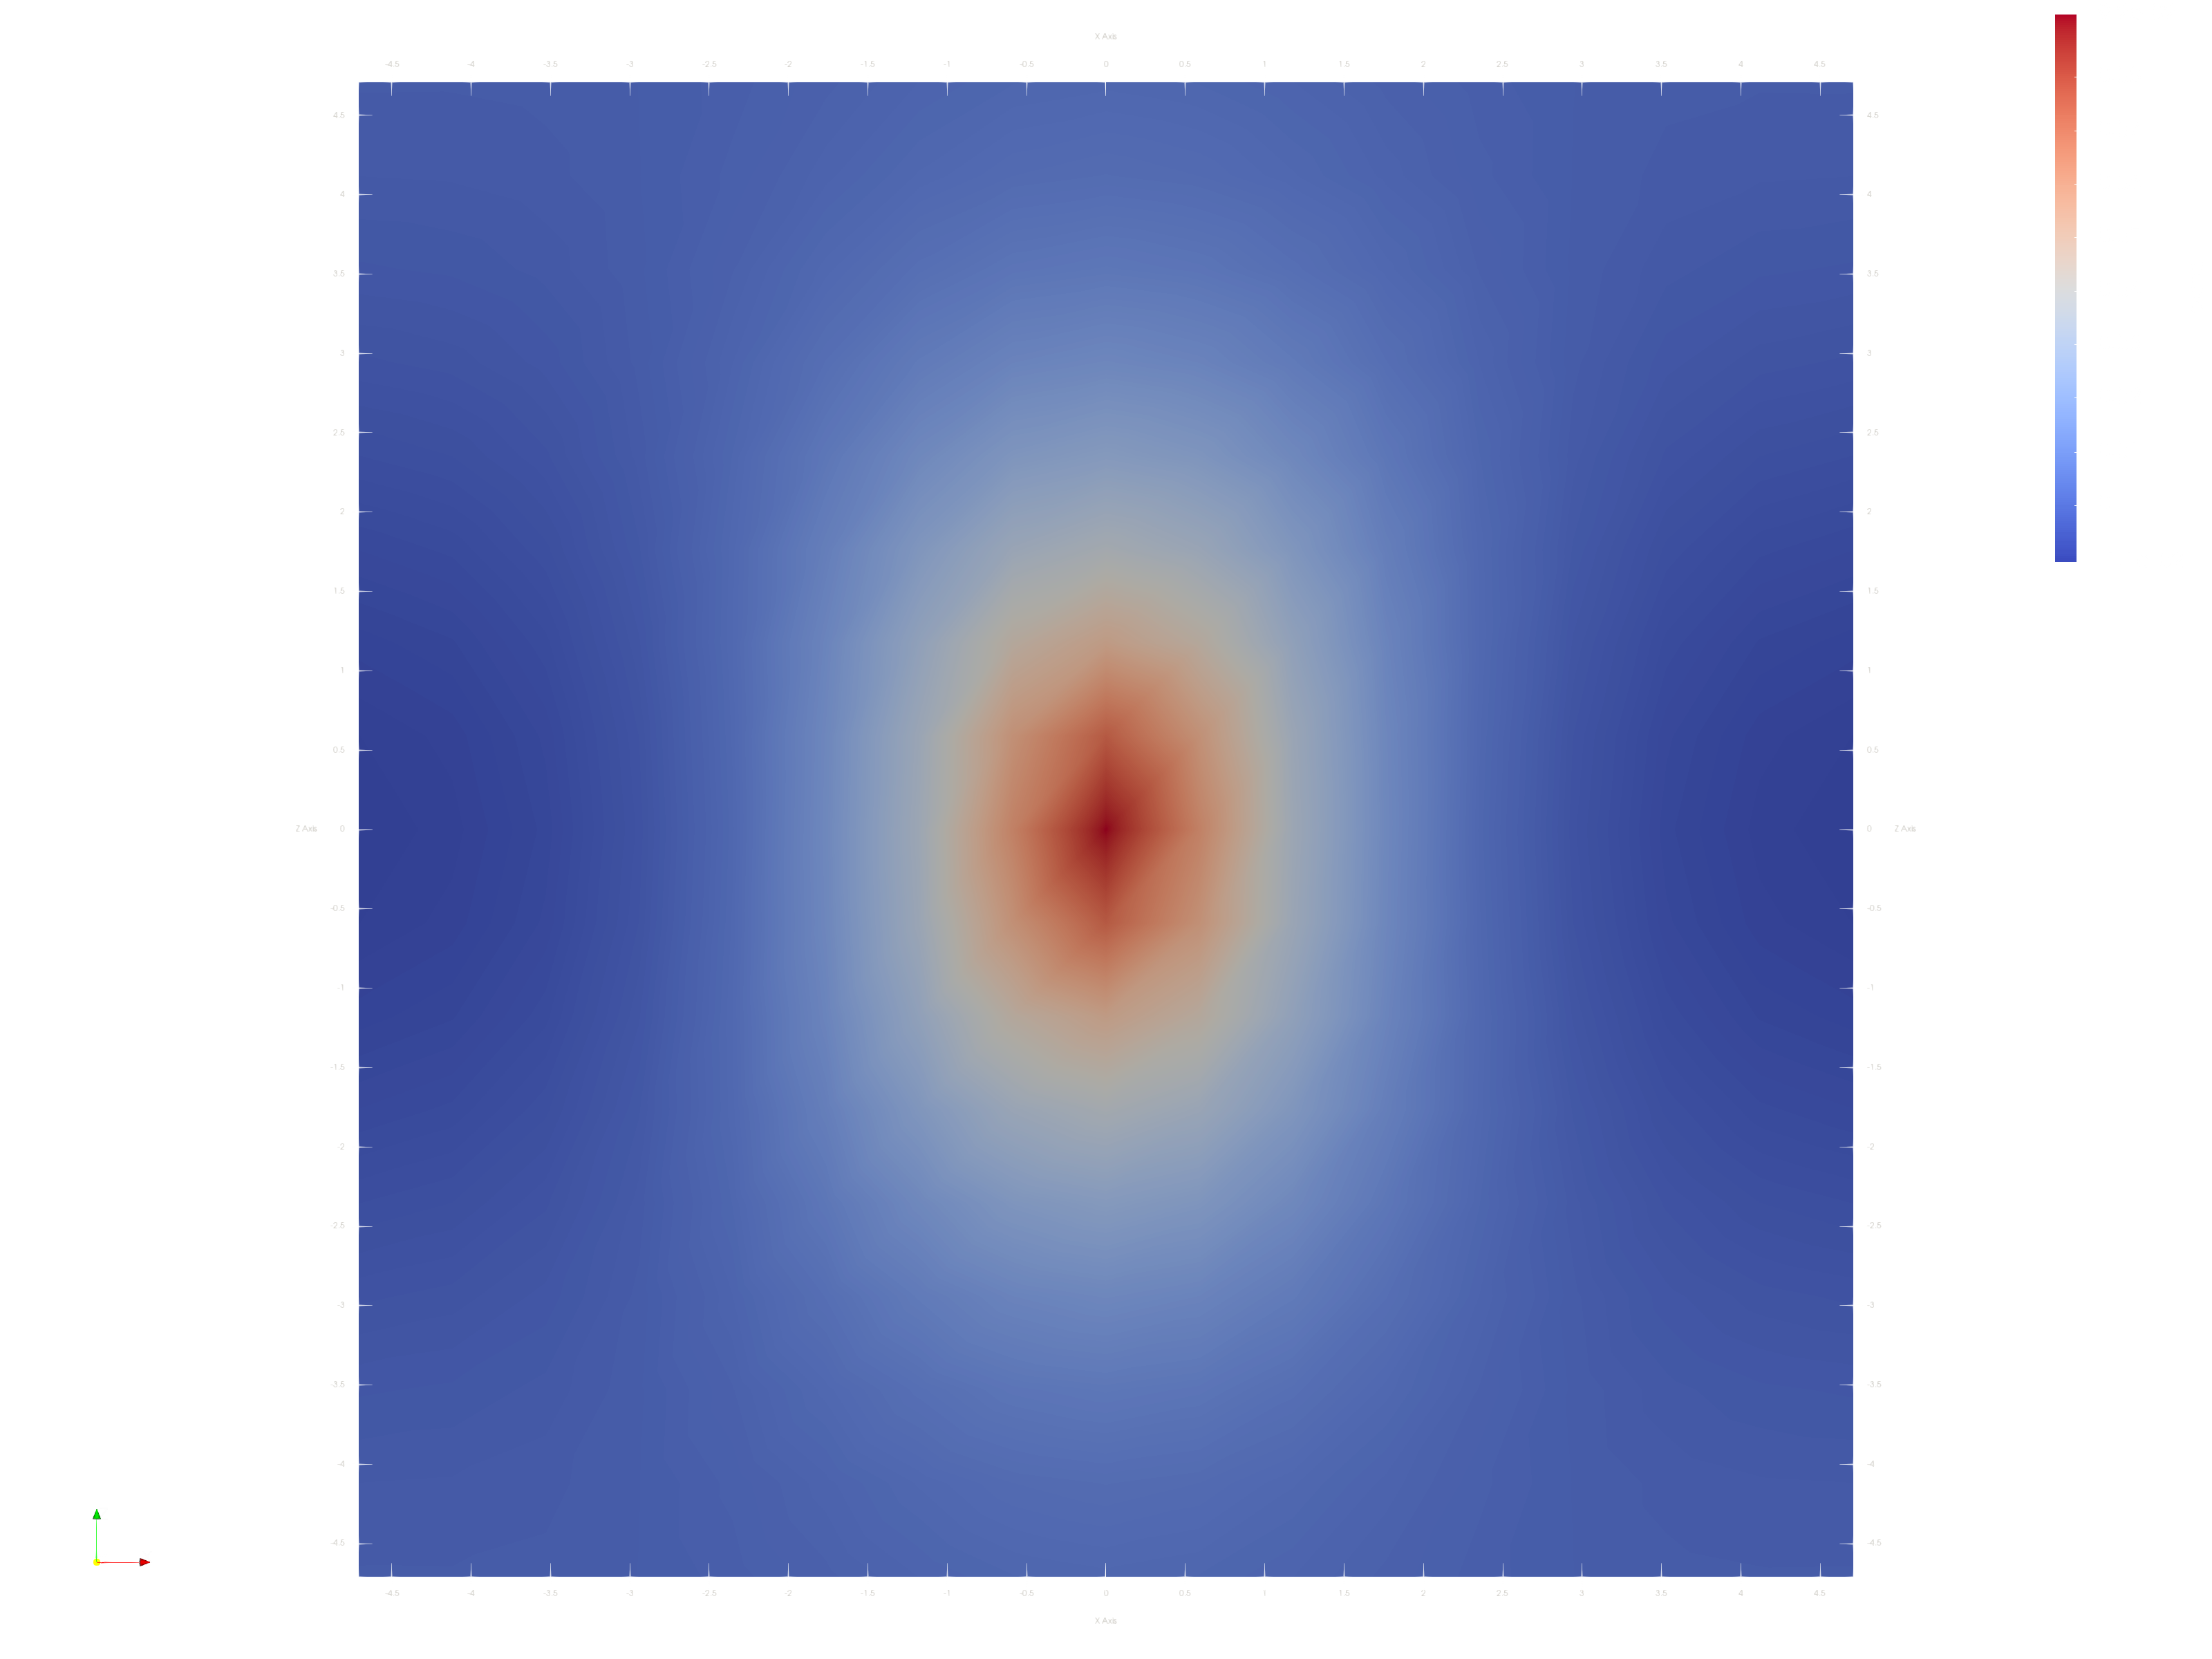
\includegraphics[width=0.32\linewidth]{images/kriging/3components/exact_cov_33_yy.png}}
        \hfill
        \subcaptionbox{$R_{zz}$ $z$-нормаль \label{img:kriging_exact_cov_r_33}} 
        {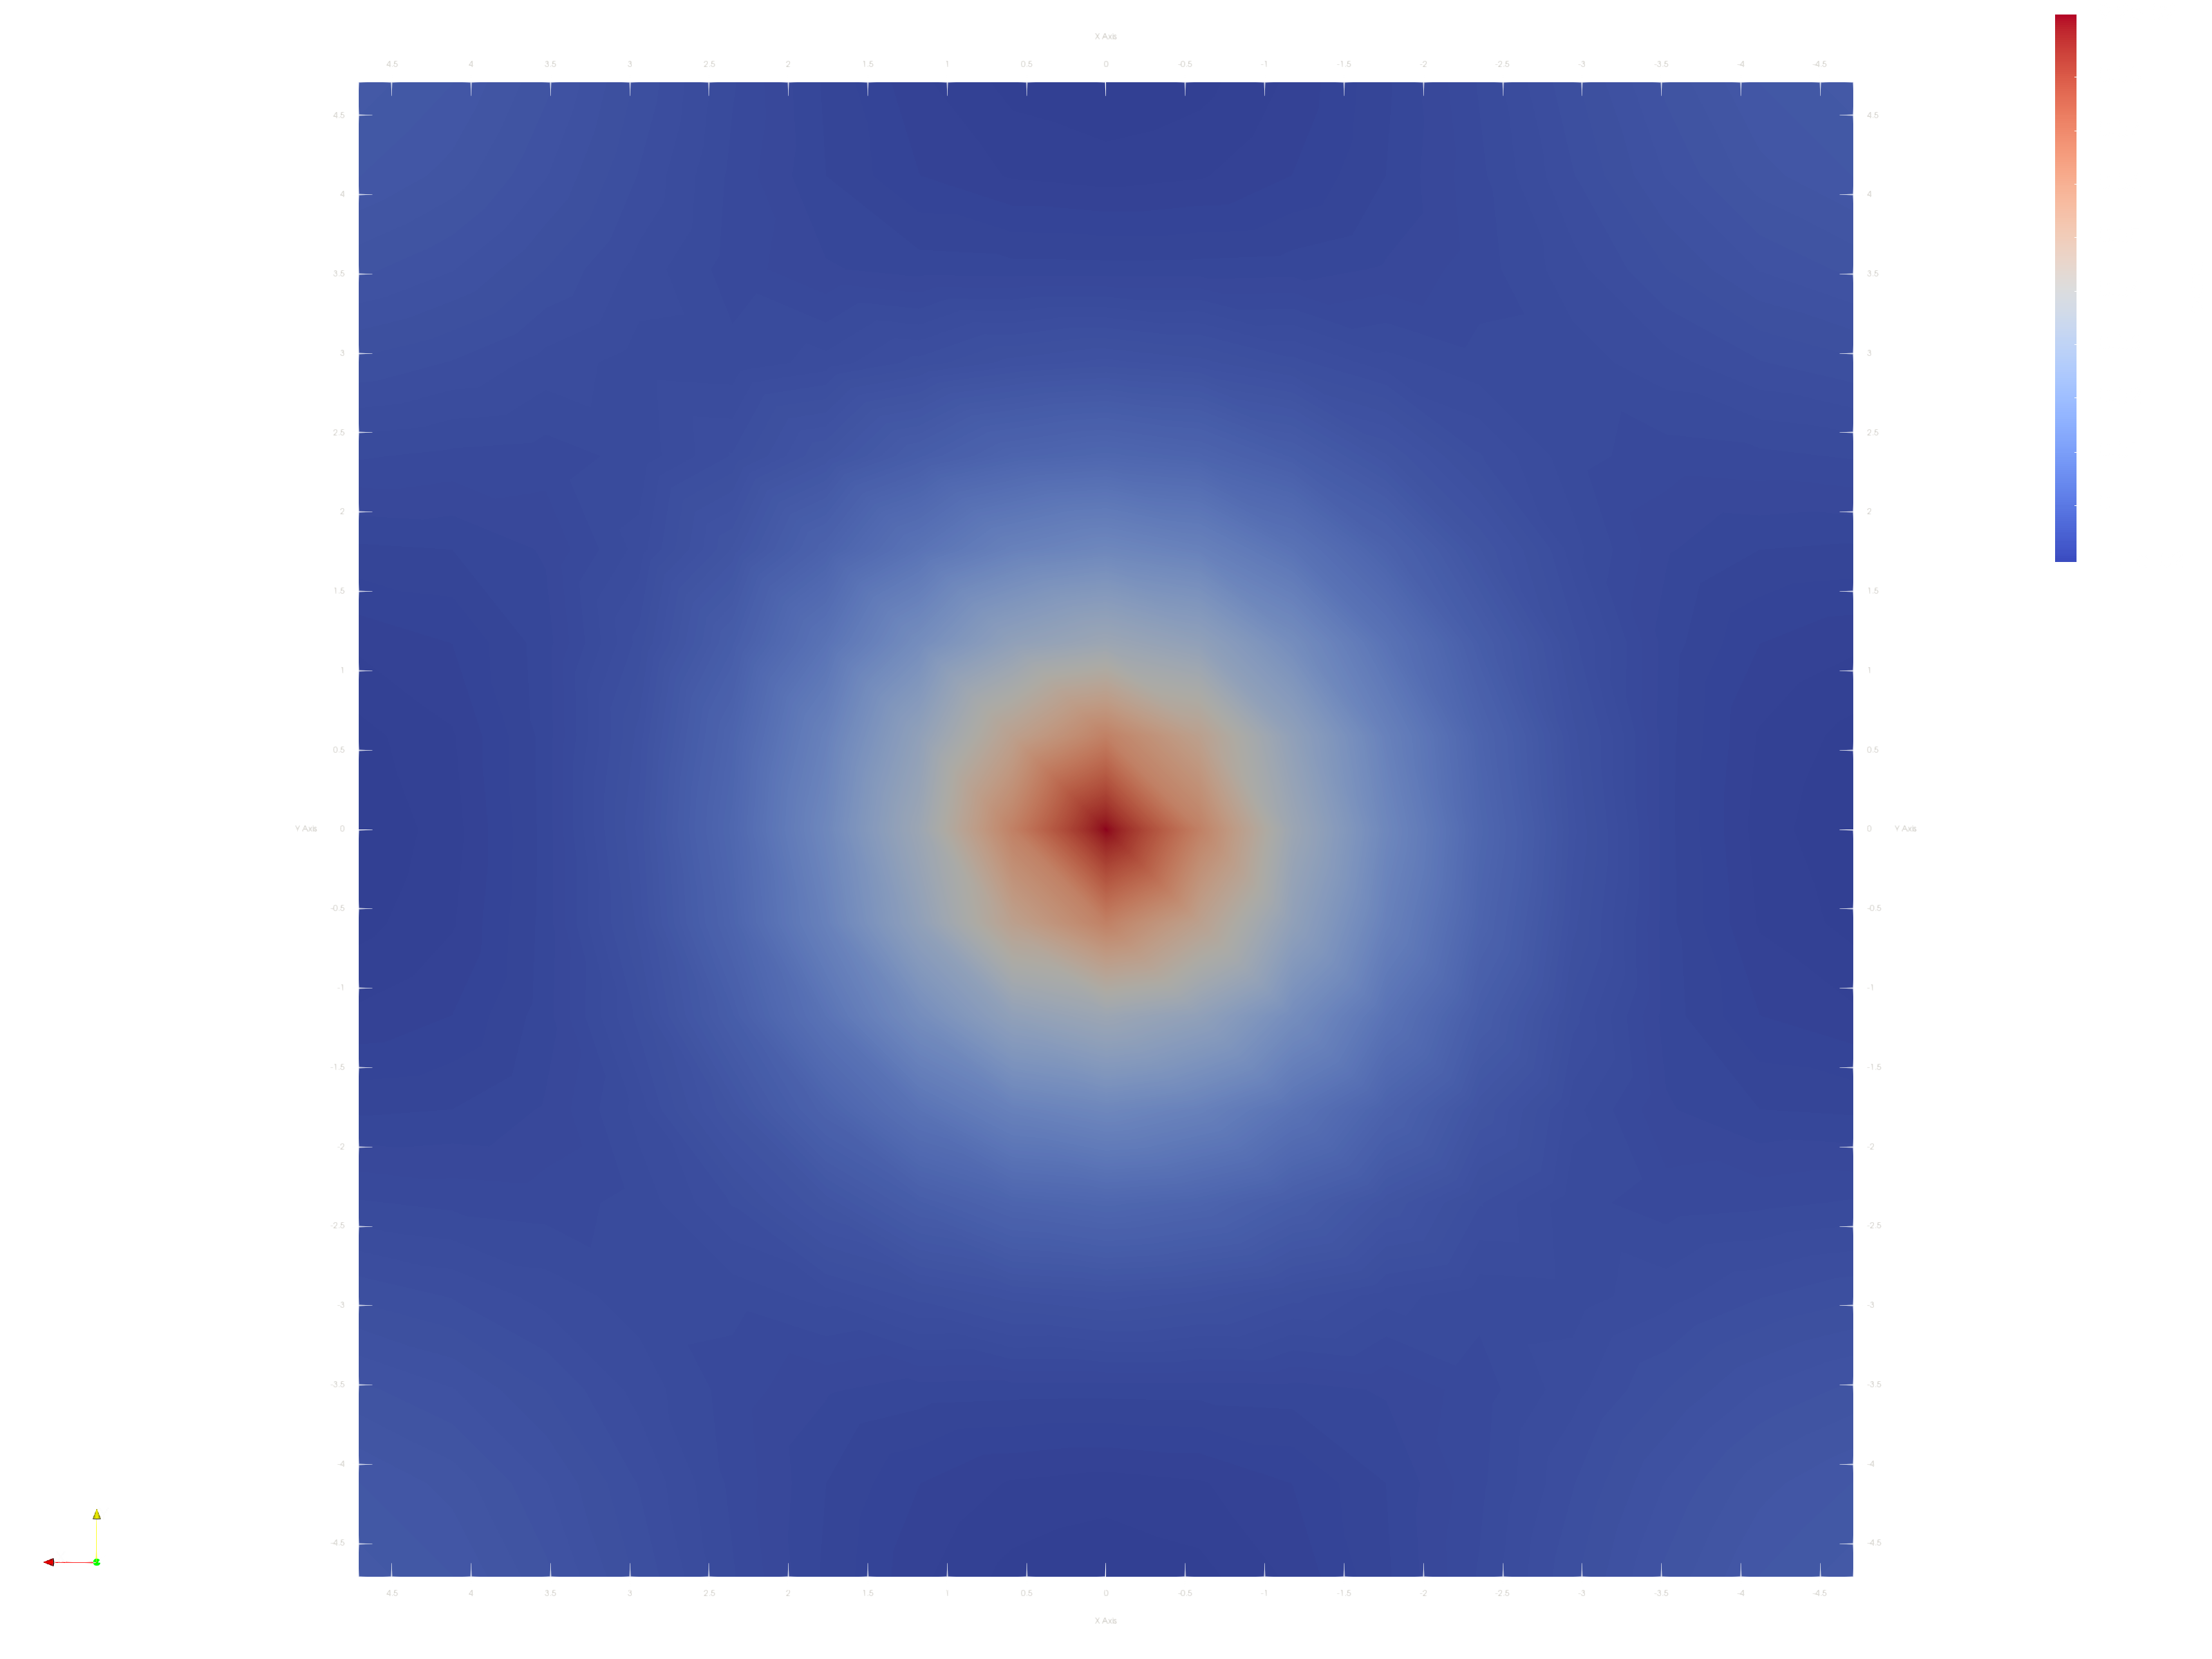
\includegraphics[width=0.32\linewidth]{images/kriging/3components/exact_cov_33_zz.png}}
        \hfill
    }
    
    \onehalfspacing{}
    \caption{Ковариационные функции, заданные для применения трёхмерного стохастического метода}
    \label{img:exact_covariance_comparison_heat_maps}  
\end{figure}

Первое, что необходимо заметить, это пространственное вытягивание компонент тензора в смежных плоскостях, в плоскостях, нормальных к текущей компоненте наблюдается симметрия ковариационной функции. При сравнении с численно полученным результатом также учтём это. Вне диагональные компоненты не представлены, так как их значение можно считать нулевыми.

Ниже представлены графики пространственной ковариации рассчитанные на 10000 реализаций полей флуктуаций полученные в результате трёхмерного стохастического моделирования. На рисунках представлены значения вдоль диагонали куба от точки $\{-5, -5, -5\}$ до точки $\{ 5, 5, 5 \}$ и значения вдоль осей координат.

%
% Ковариация по осям координат
%
\begin{figure}[ht] 
  \center
  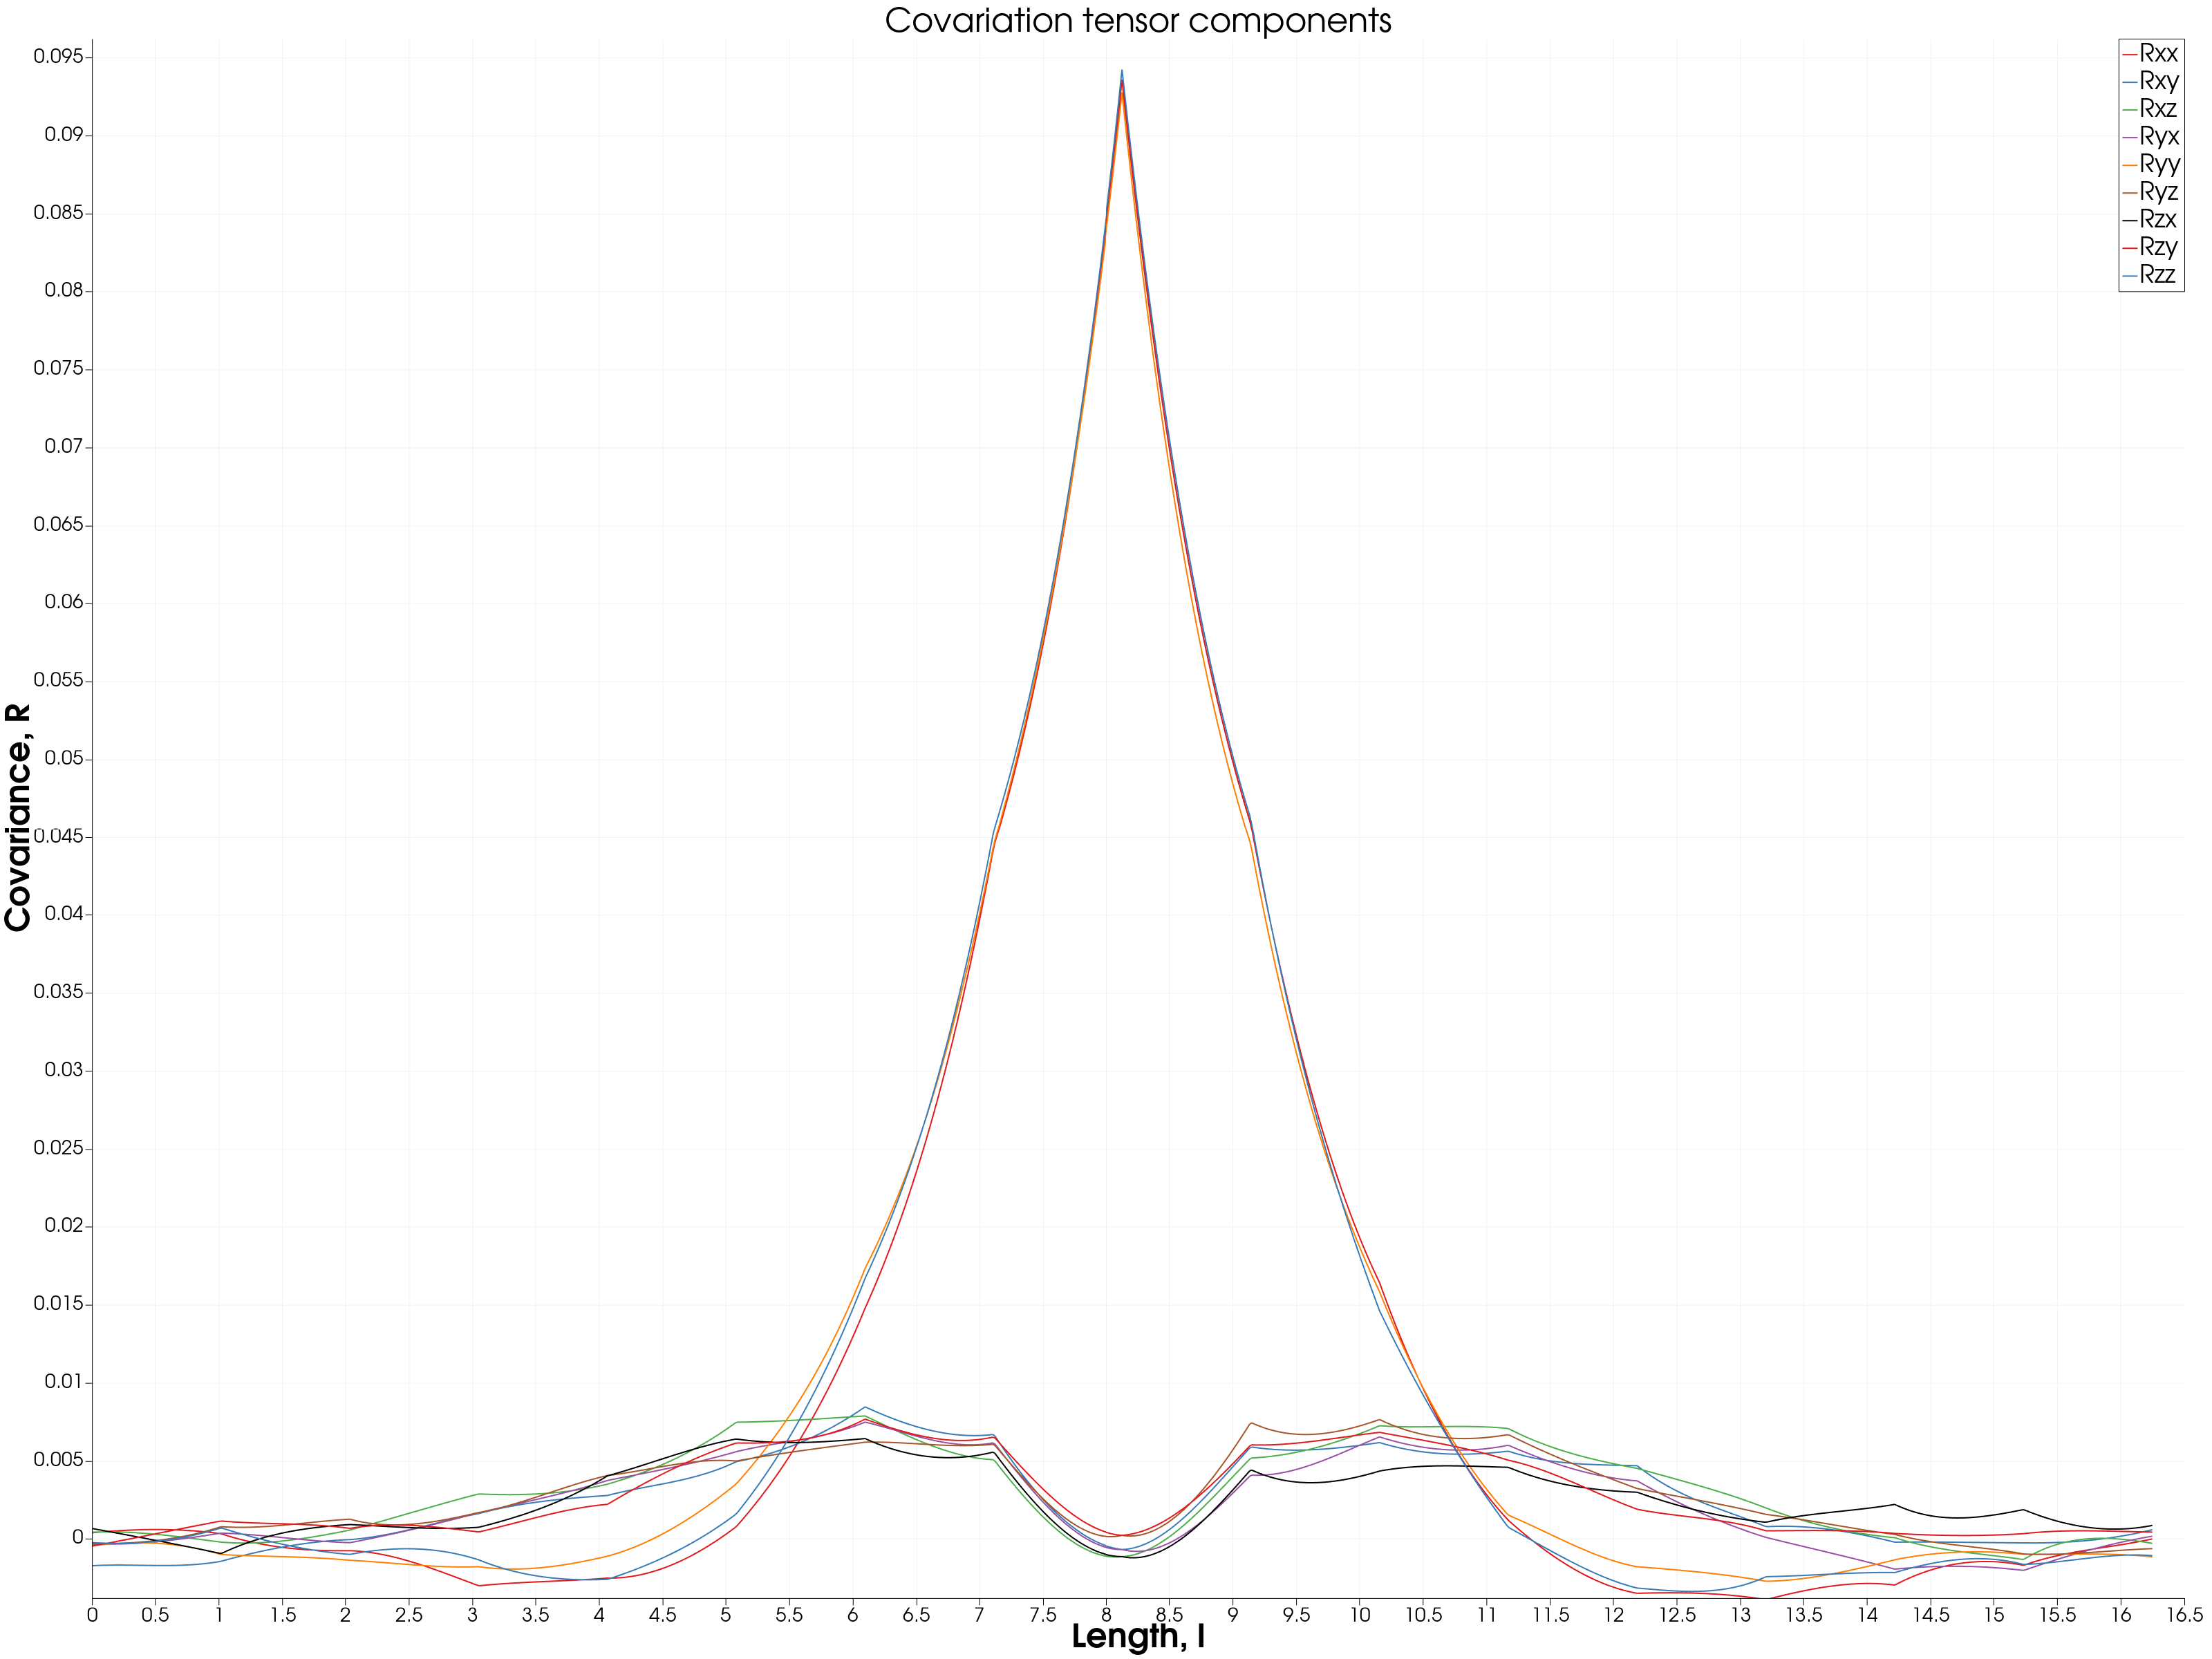
\includegraphics [width=0.8\linewidth] {images/kriging/3components/calculated_all_diag.png}
  \caption{Расчётная ковариационная функция $R_{ik}$ на основе стохастического метода вдоль диагонали области } 
  \label{img:kriging_covariances_diag}  
\end{figure}

\begin{figure}[ht] 
  \center
  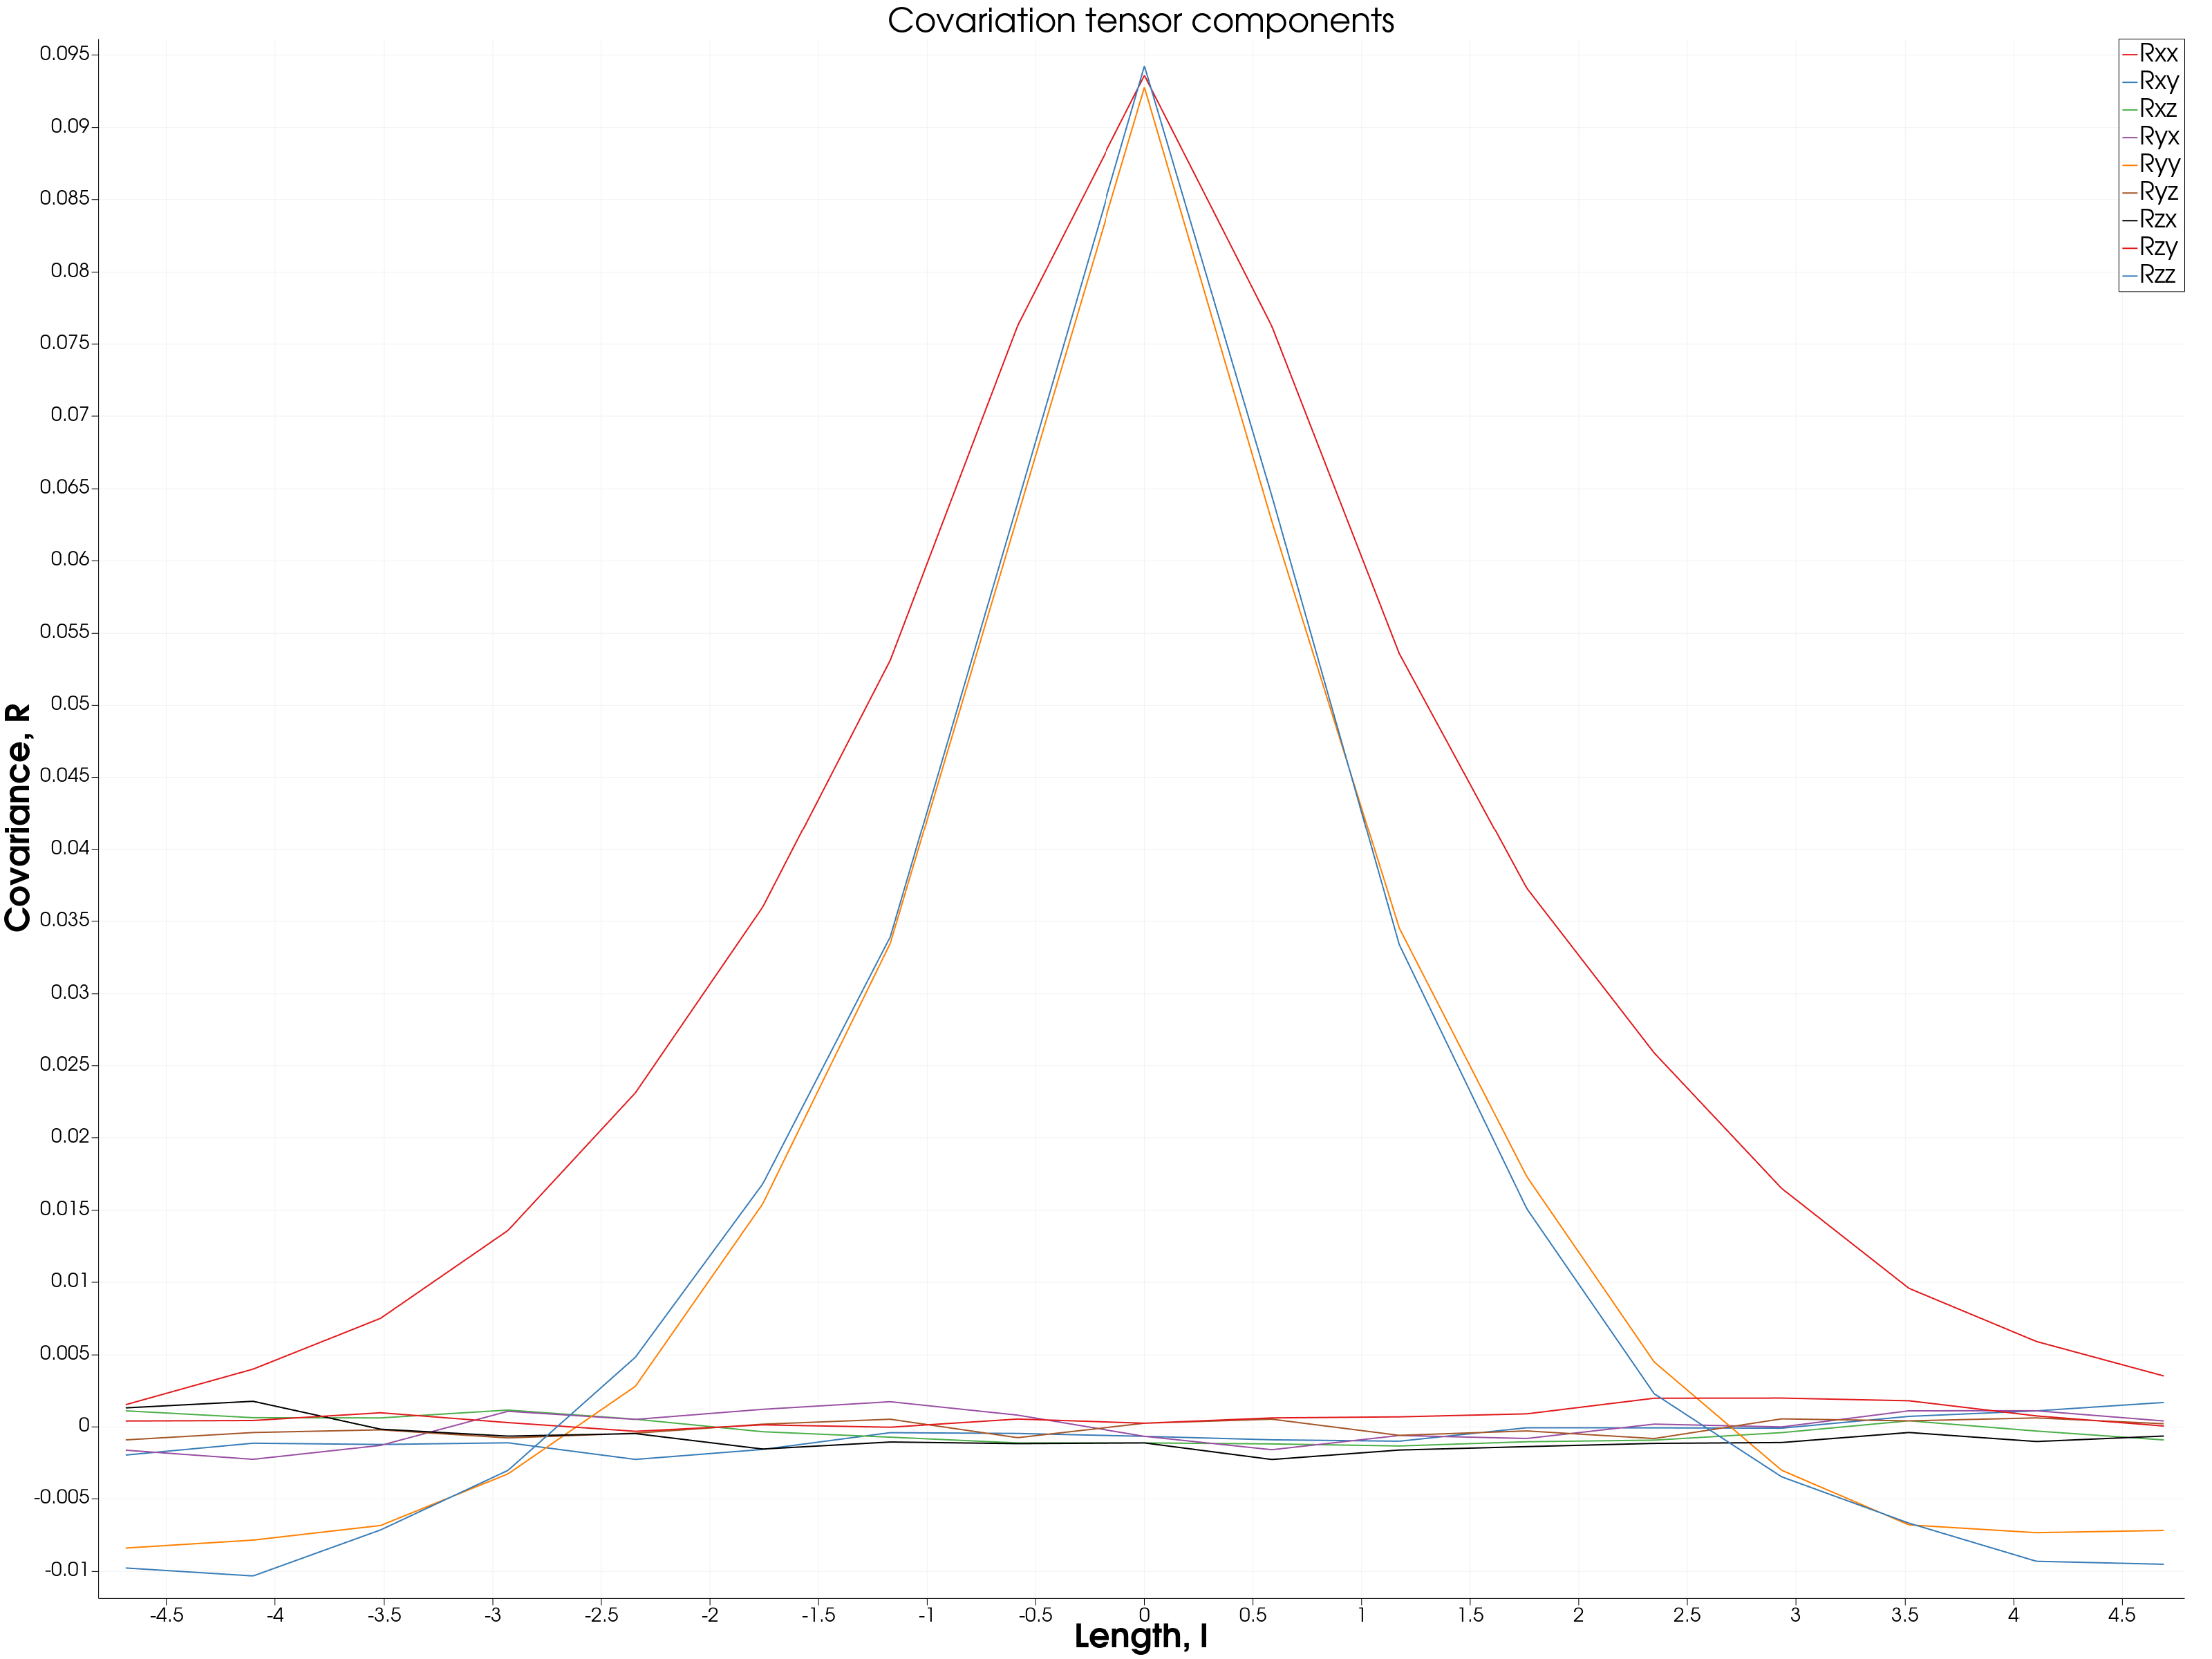
\includegraphics [width=0.8\linewidth] {images/kriging/3components/calculated_all_x.png}
  \caption{Расчётная ковариационная функция $R_{ik}$ на основе стохастического метода вдоль оси $x$ области } 
  \label{img:kriging_covariances_diag}  
\end{figure}

\begin{figure}[ht] 
  \center
  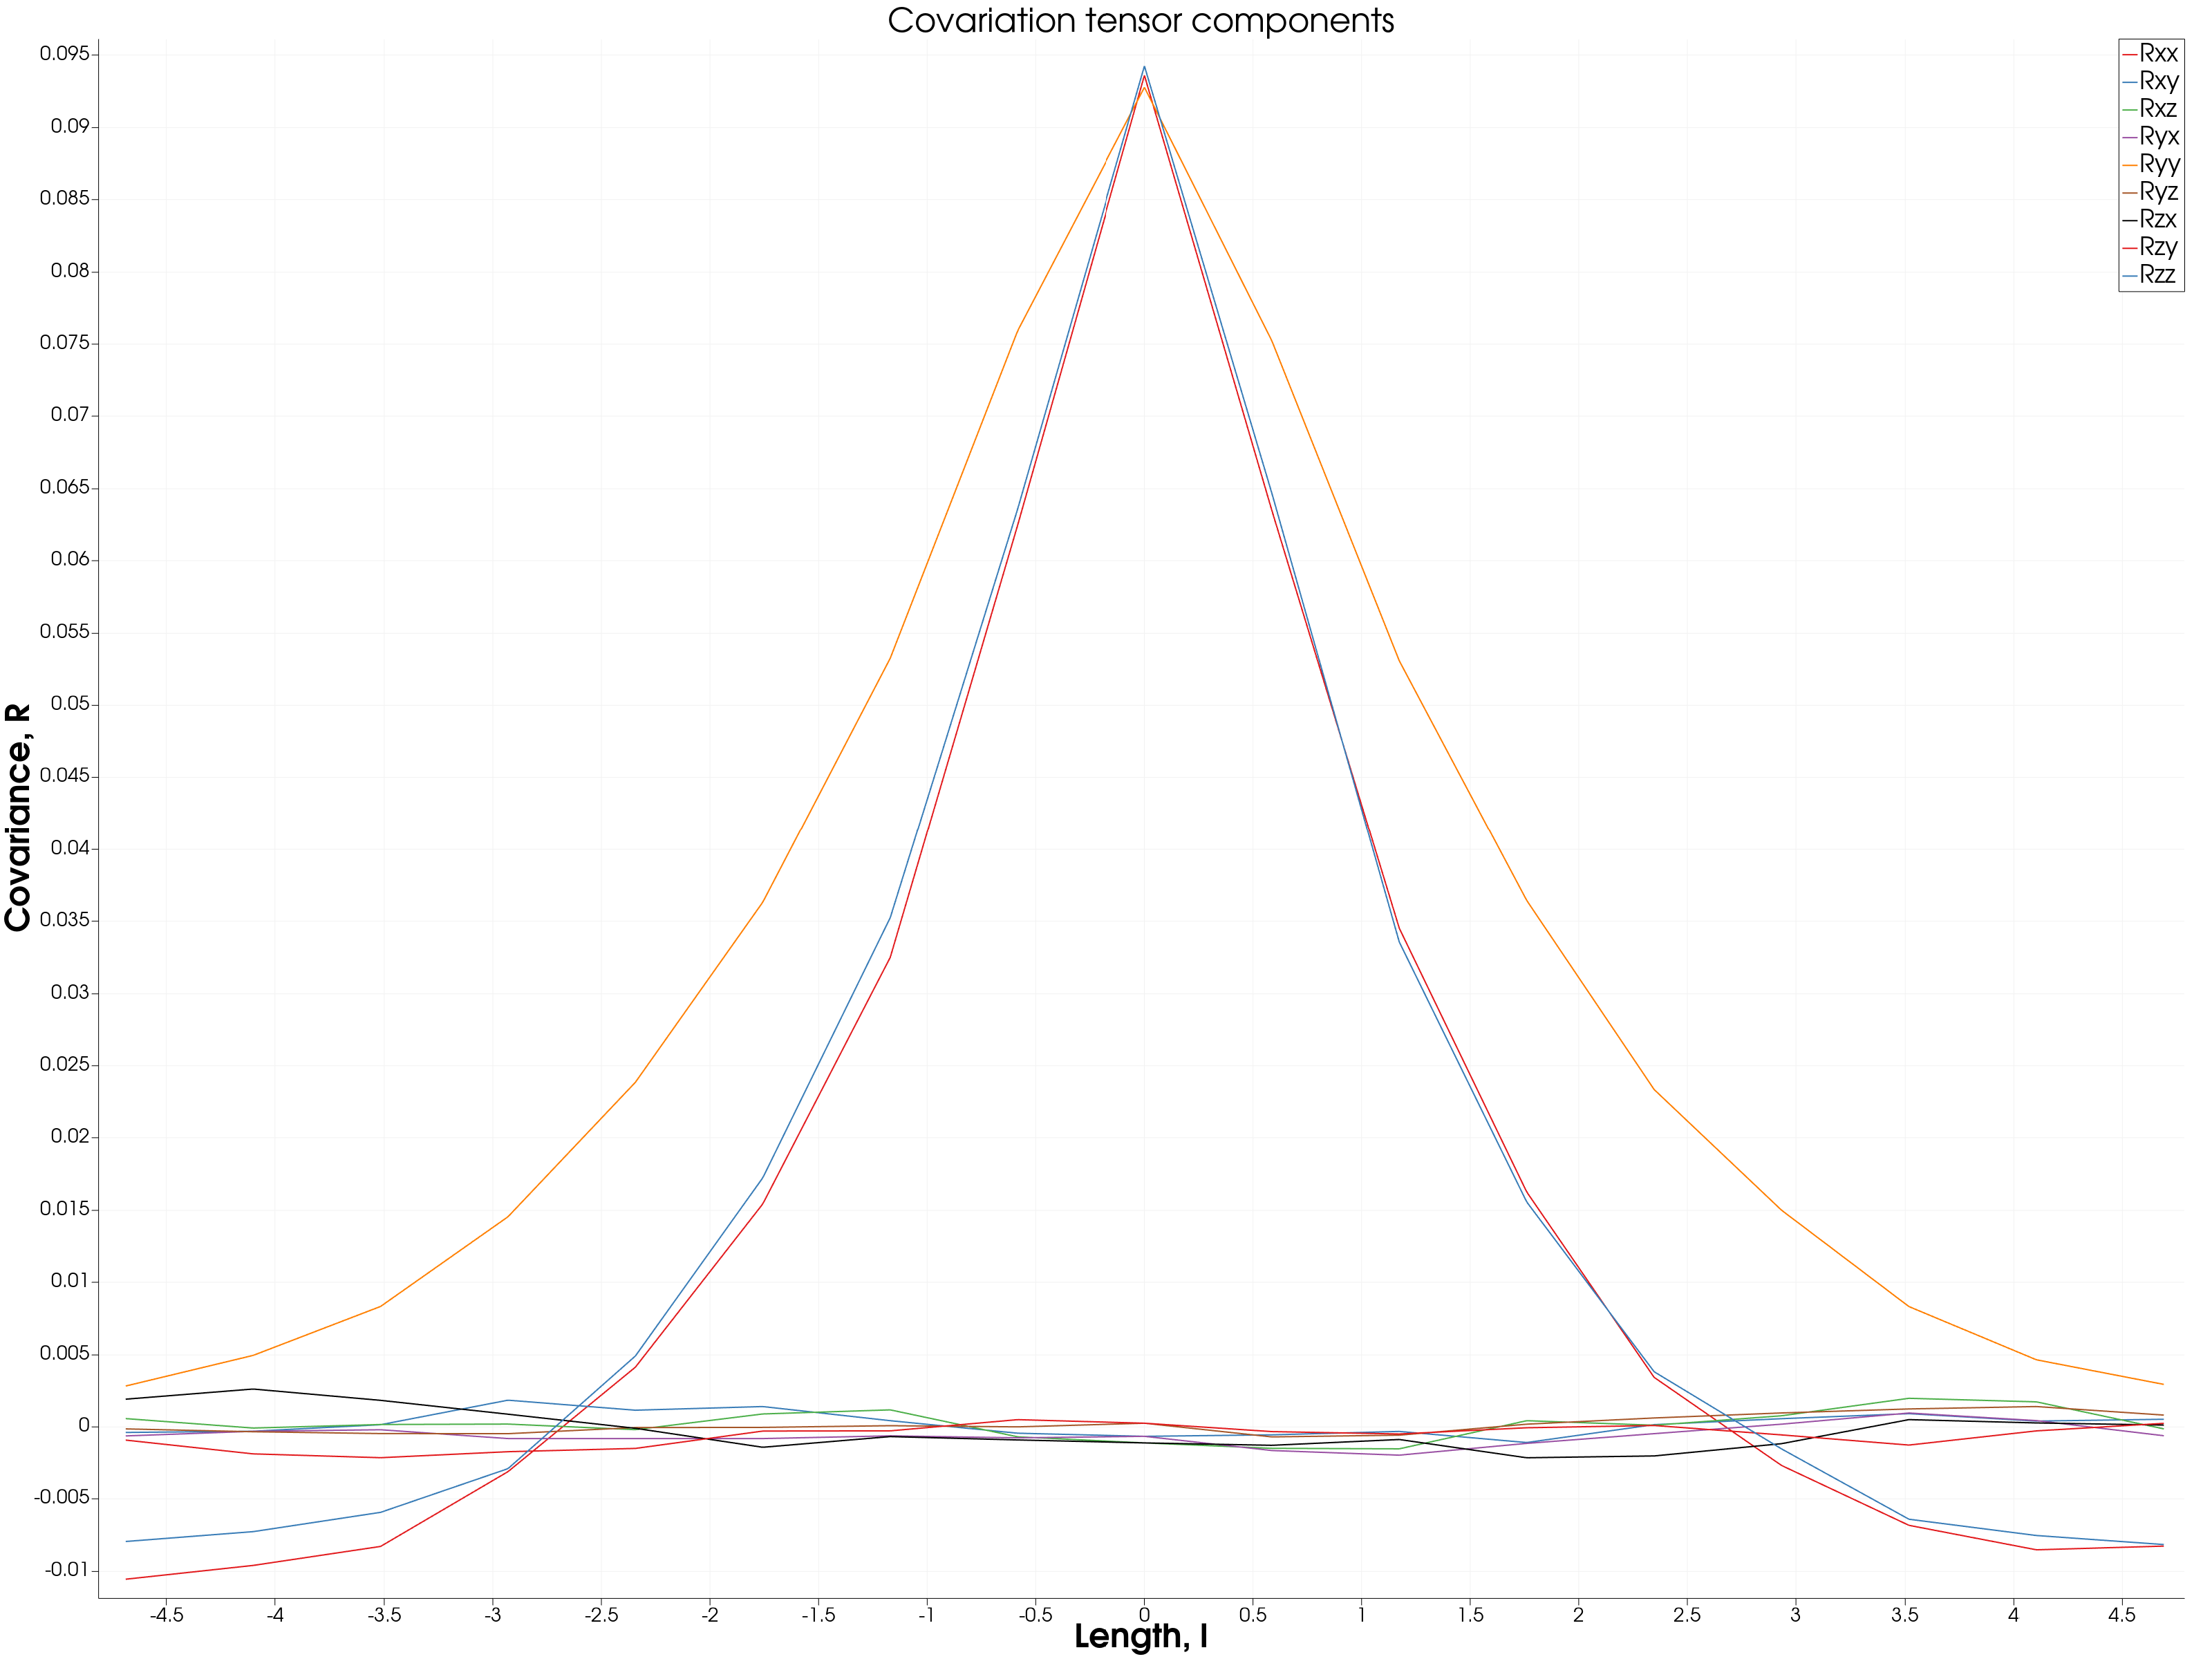
\includegraphics [width=0.8\linewidth] {images/kriging/3components/calculated_all_y.png}
  \caption{Расчётная ковариационная функция $R_{ik}$ на основе стохастического метода вдоль оси $y$ области } 
  \label{img:kriging_covariances_diag}  
\end{figure}

\begin{figure}[ht] 
  \center
  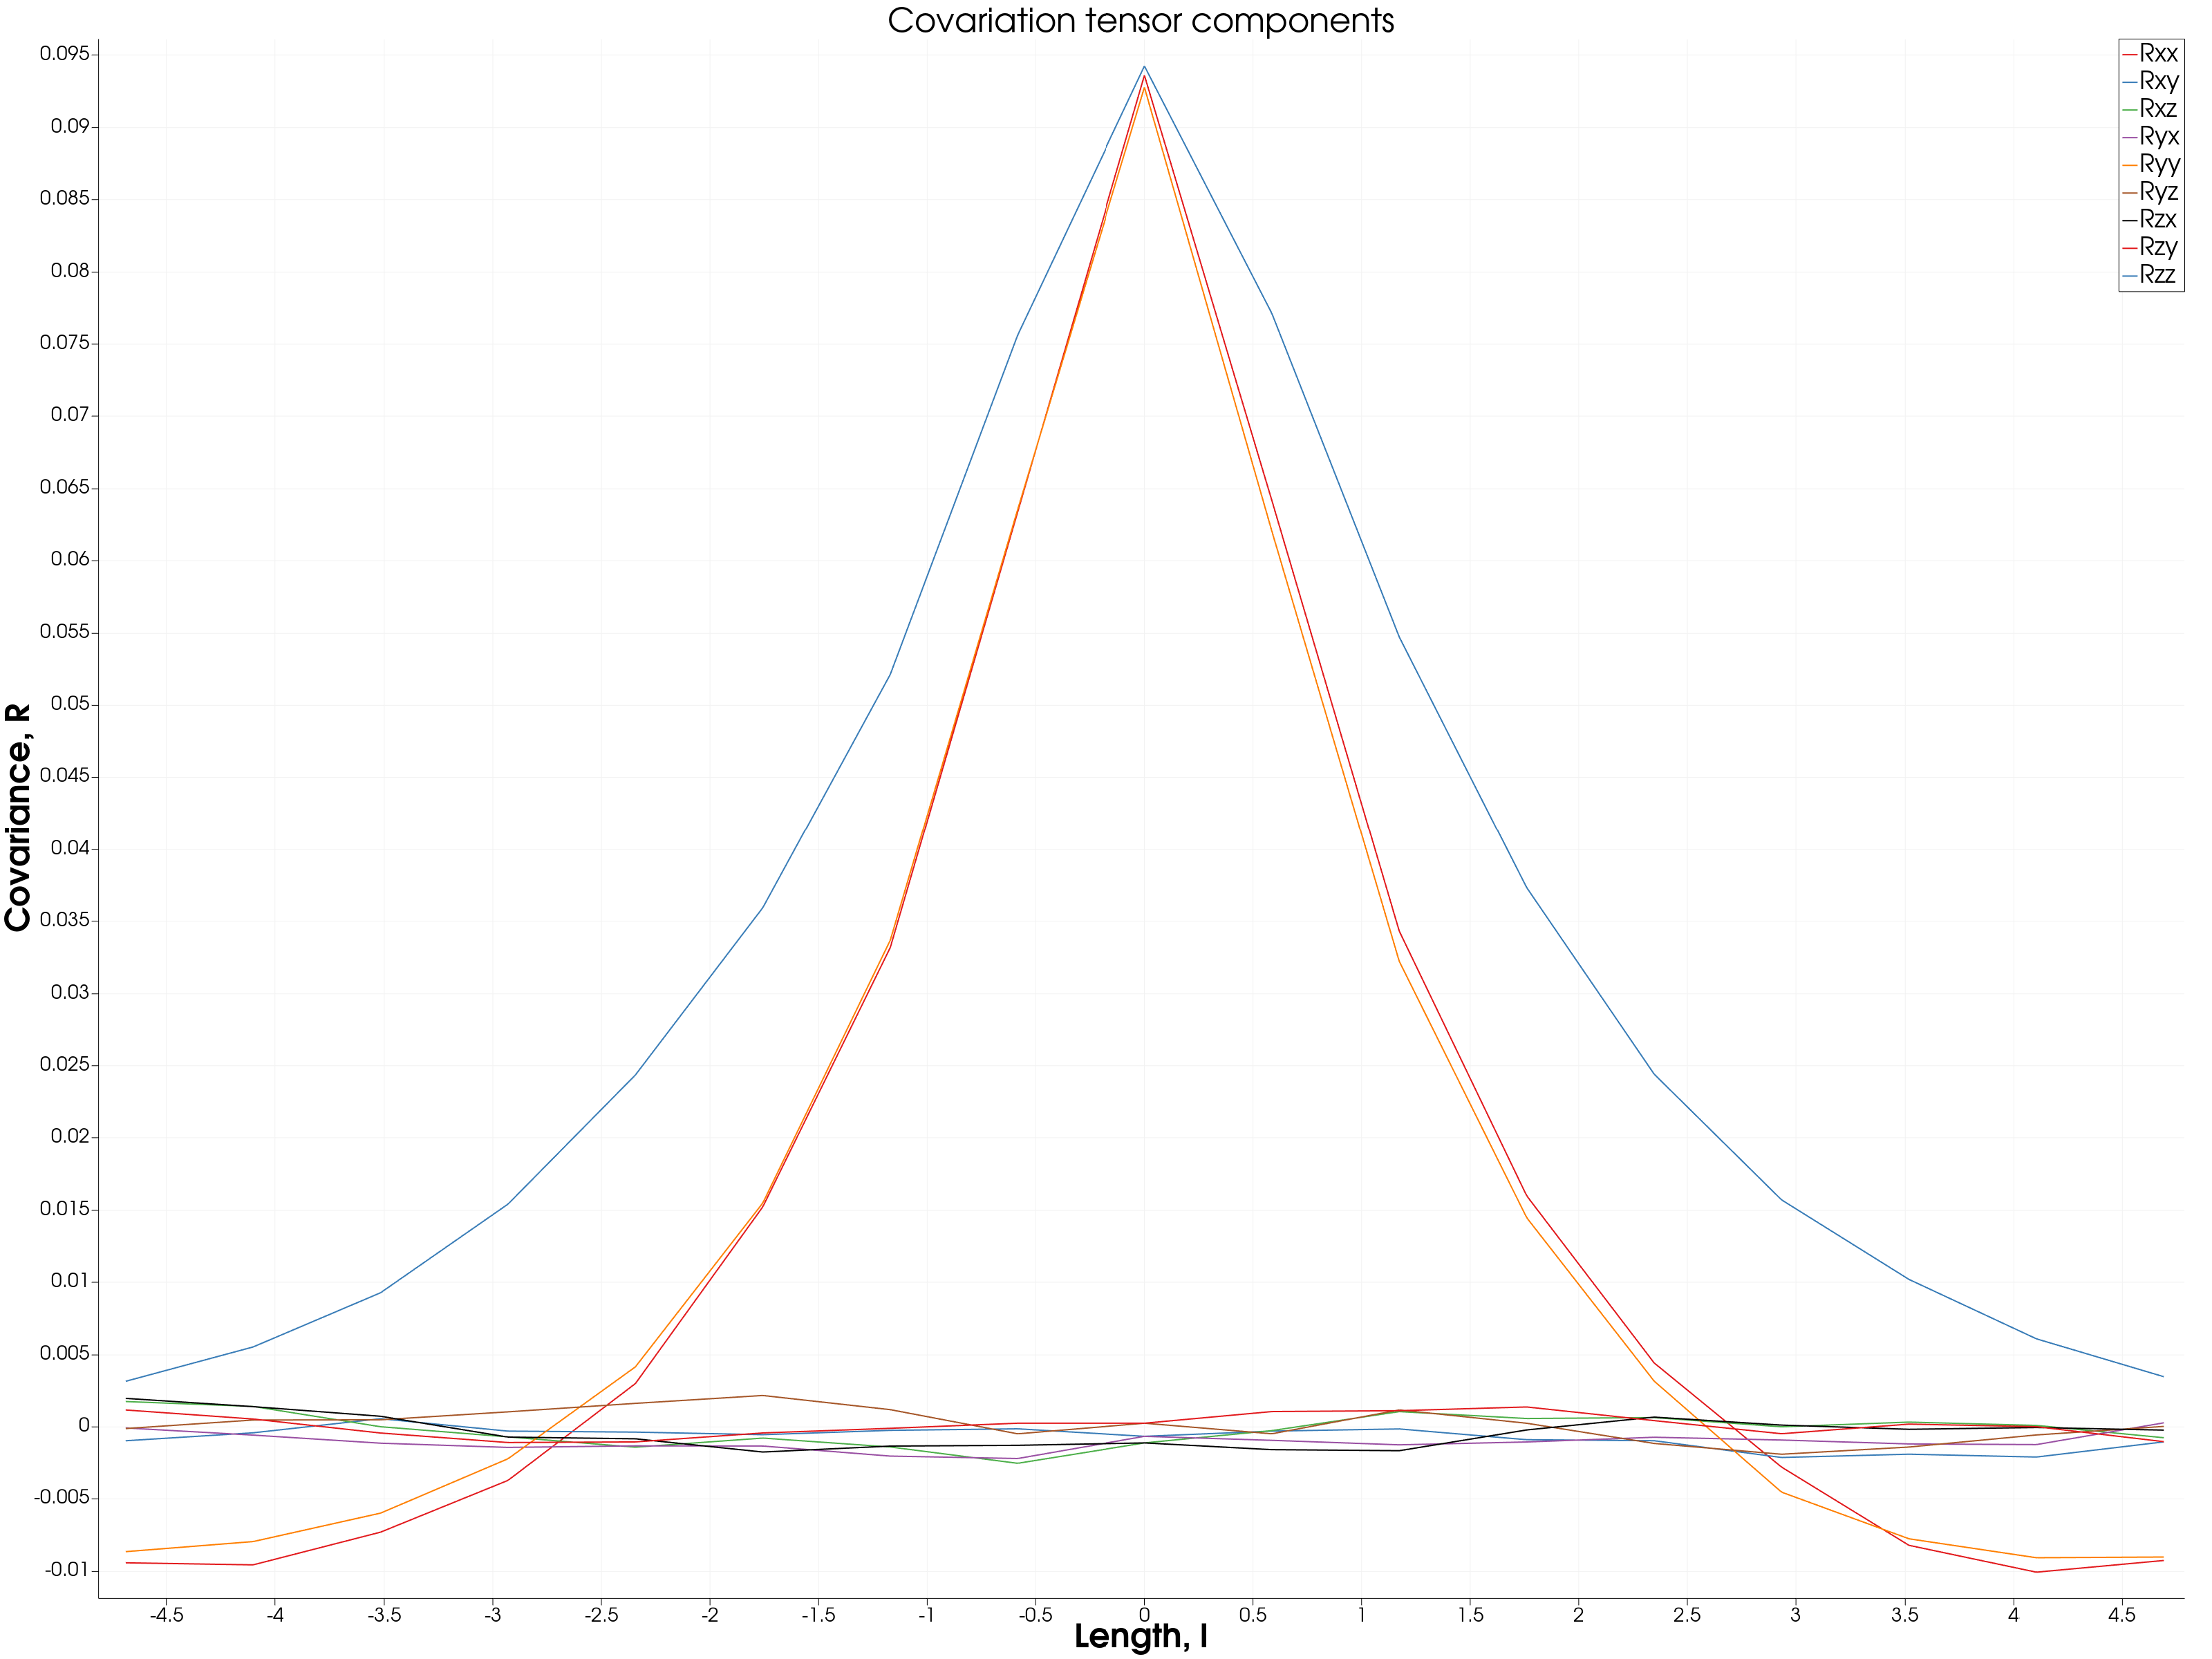
\includegraphics [width=0.8\linewidth] {images/kriging/3components/calculated_all_z.png}
  \caption{Расчётная ковариационная функция $R_{ik}$ на основе стохастического метода вдоль оси $z$ области } 
  \label{img:kriging_covariances_diag}  
\end{figure}

Как можно видеть из приведённых выше графиков, наблюдается вытягивание вдоль соответствующих компонент. Также наблюдается достаточно высокая визуальная симметрия относительно начала координат. С ростом расстояния наблюдаются большие отклонения ковариационной функции, связанные с тем, что выборка, на которой рассчитывались ковариационные функции конечна. Ниже представлены сравнения полученных ковариационны функций для диагональных компонент в различных направлениях с задаваемыми, а также с симметризованной относительно начала координат расчётной ковариационной функцией.

\begin{figure}[ht] 
  \center
  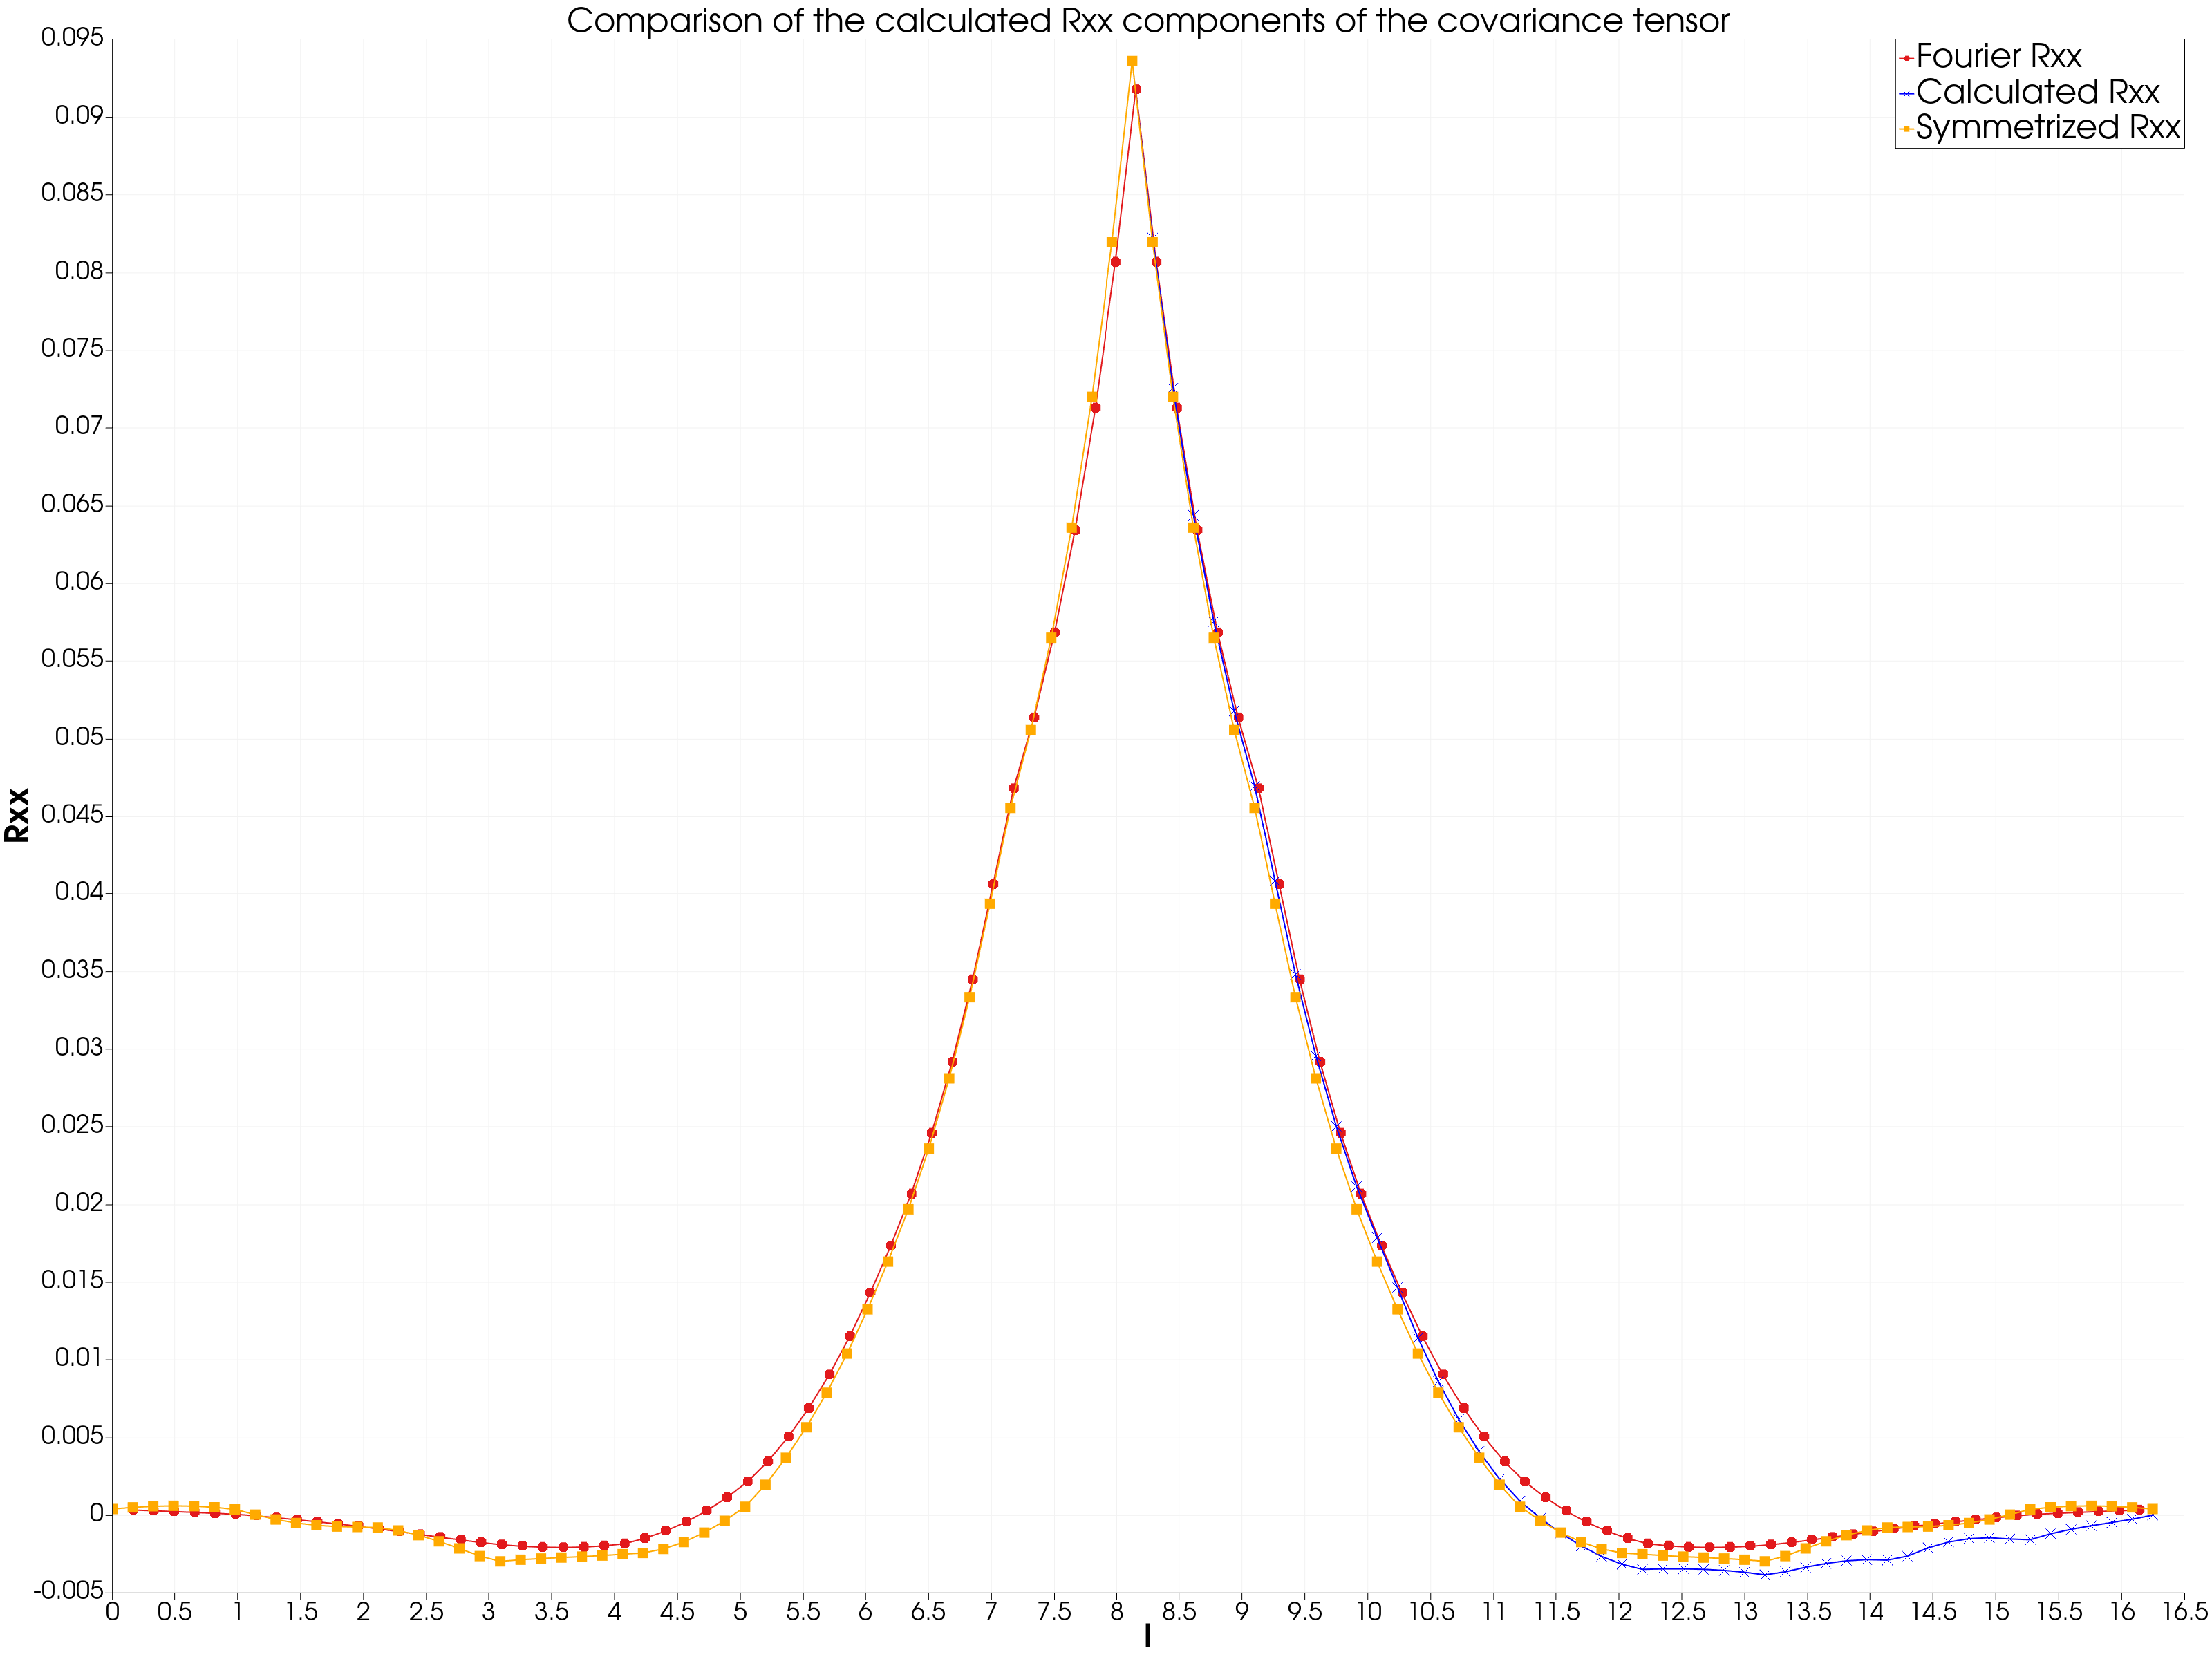
\includegraphics [width=0.8\linewidth] {images/kriging/3components/diagonal_r11_x.png}
  \caption{Расчётная ковариационная функция $R_{xx}$ на основе стохастического метода вдоль диагонали области } 
  \label{img:kriging_covariances_diag}  
\end{figure}

\begin{figure}[ht] 
  \center
  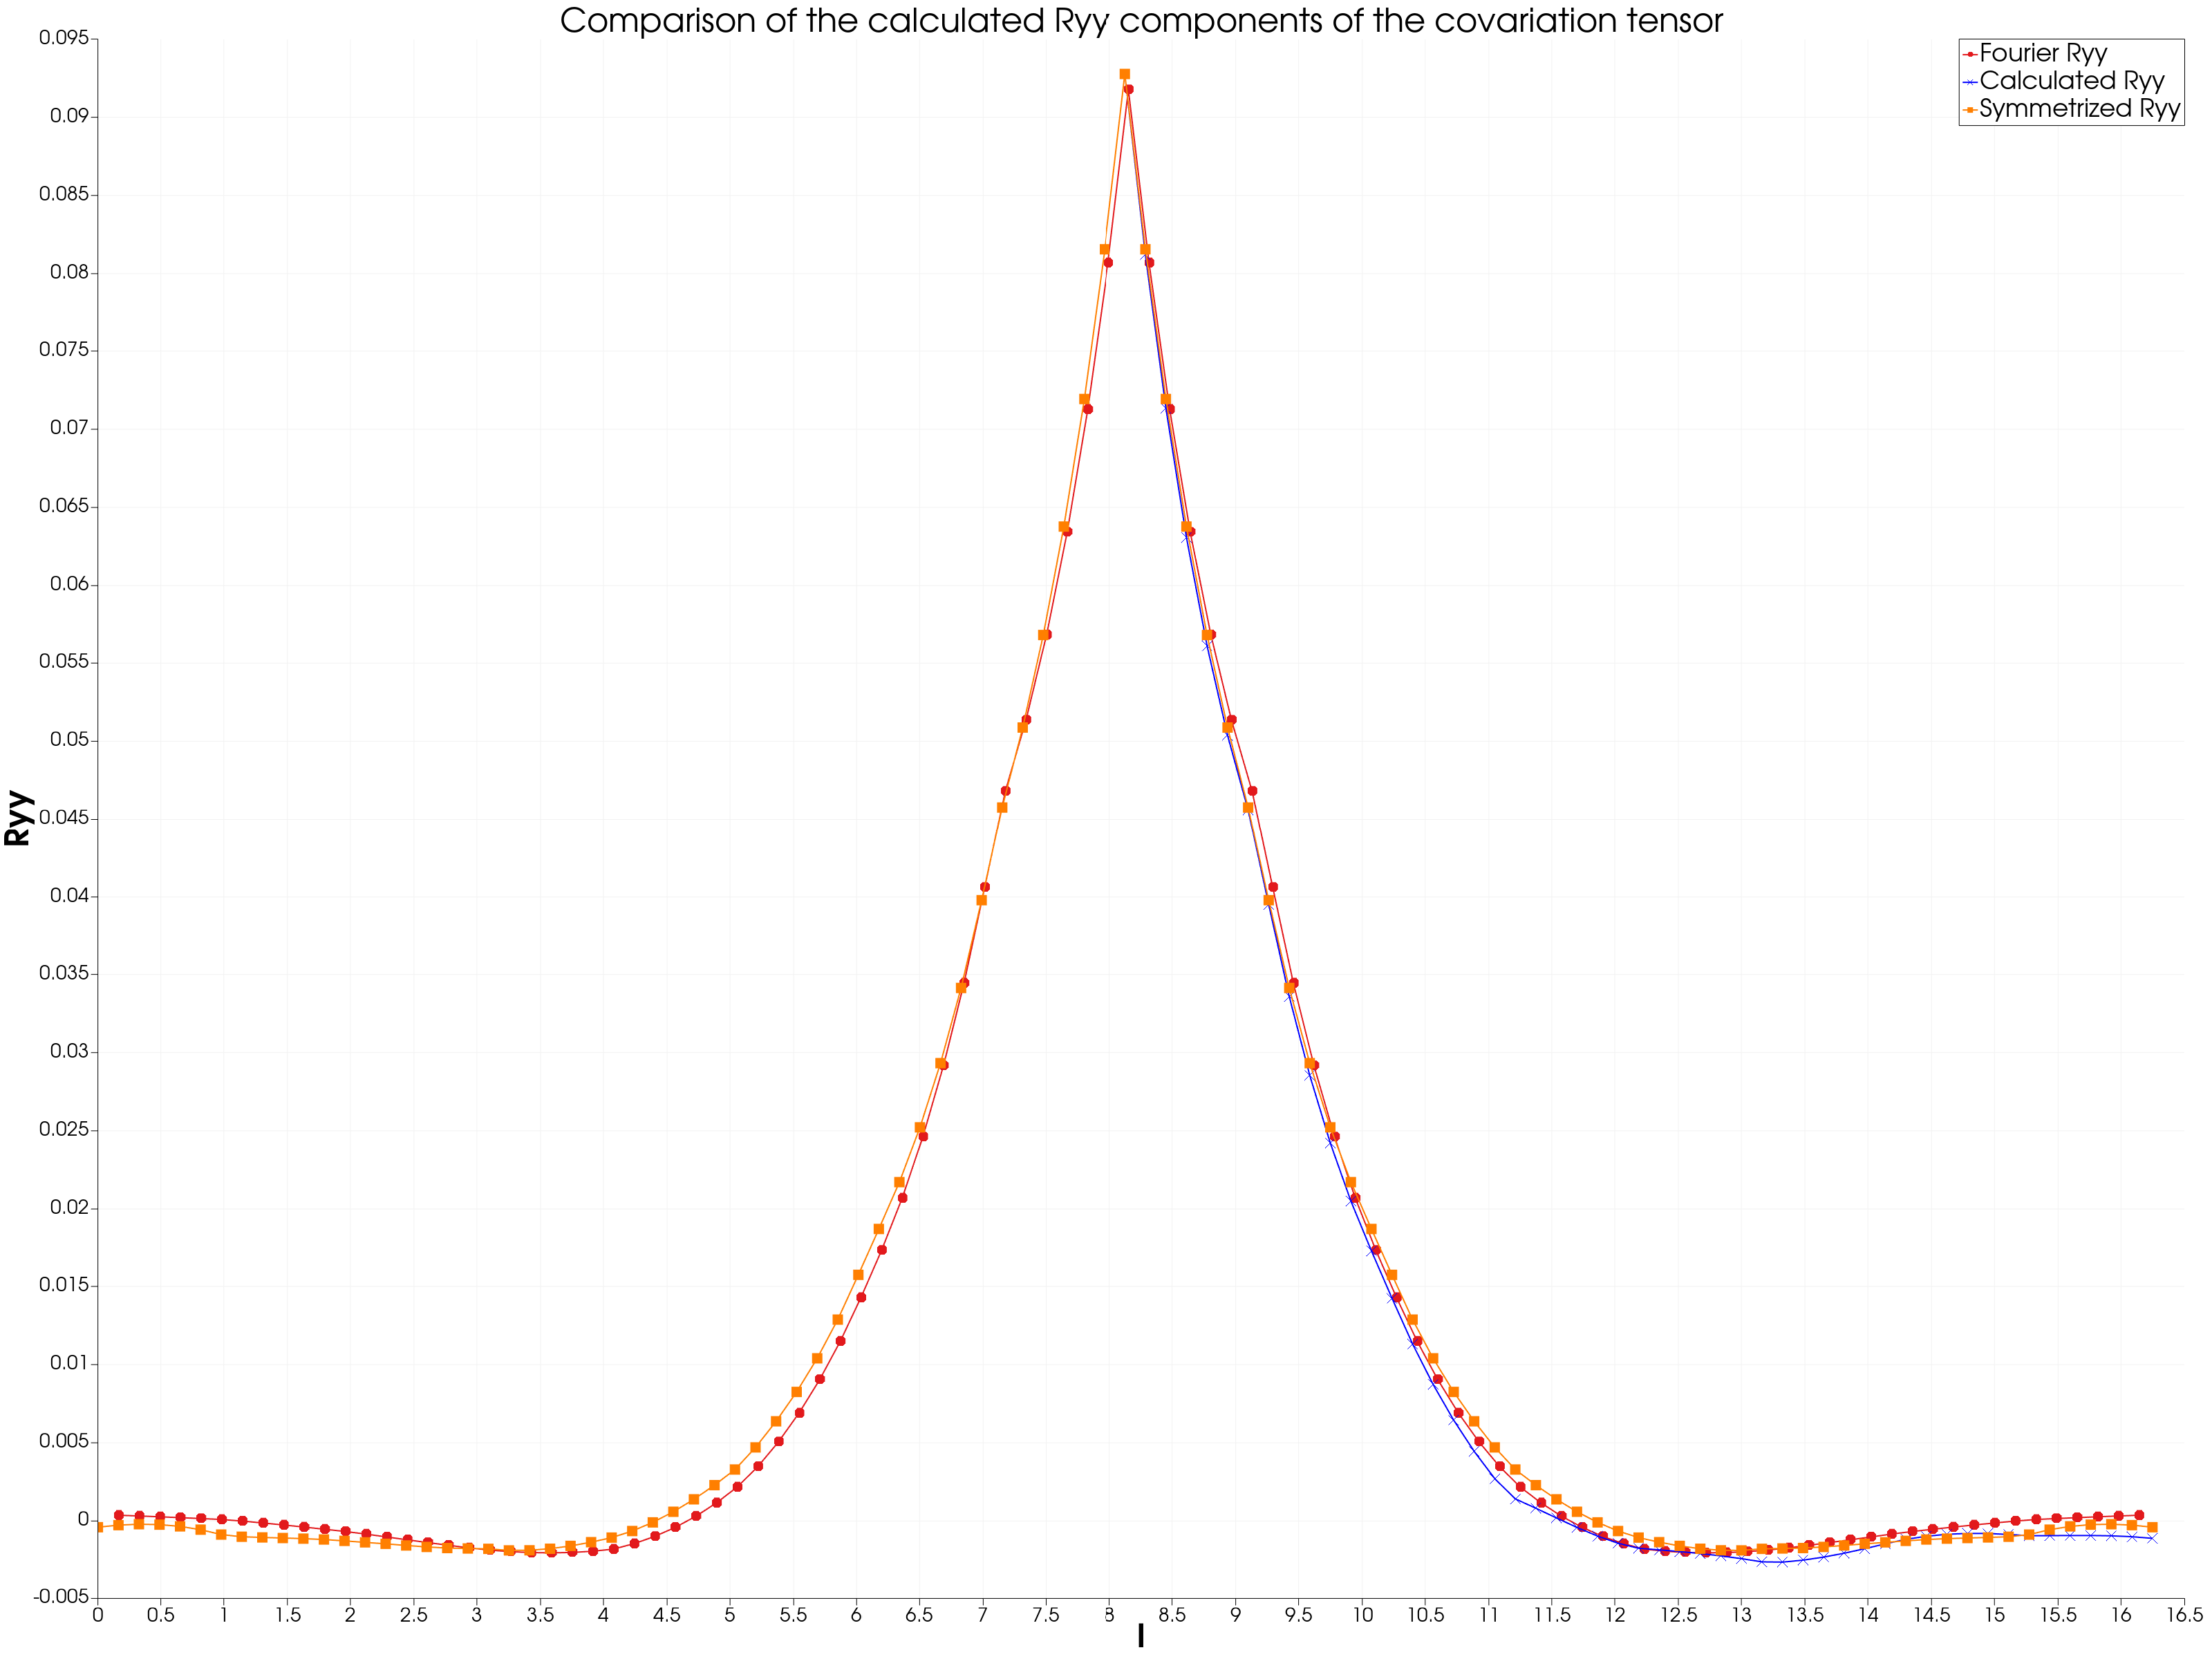
\includegraphics [width=0.8\linewidth] {images/kriging/3components/diagonal_r22_yy.png}
  \caption{Расчётная ковариационная функция $R_{yy}$ на основе стохастического метода вдоль диагонали области } 
  \label{img:kriging_covariances_diag}  
\end{figure}

\begin{figure}[ht] 
  \center
  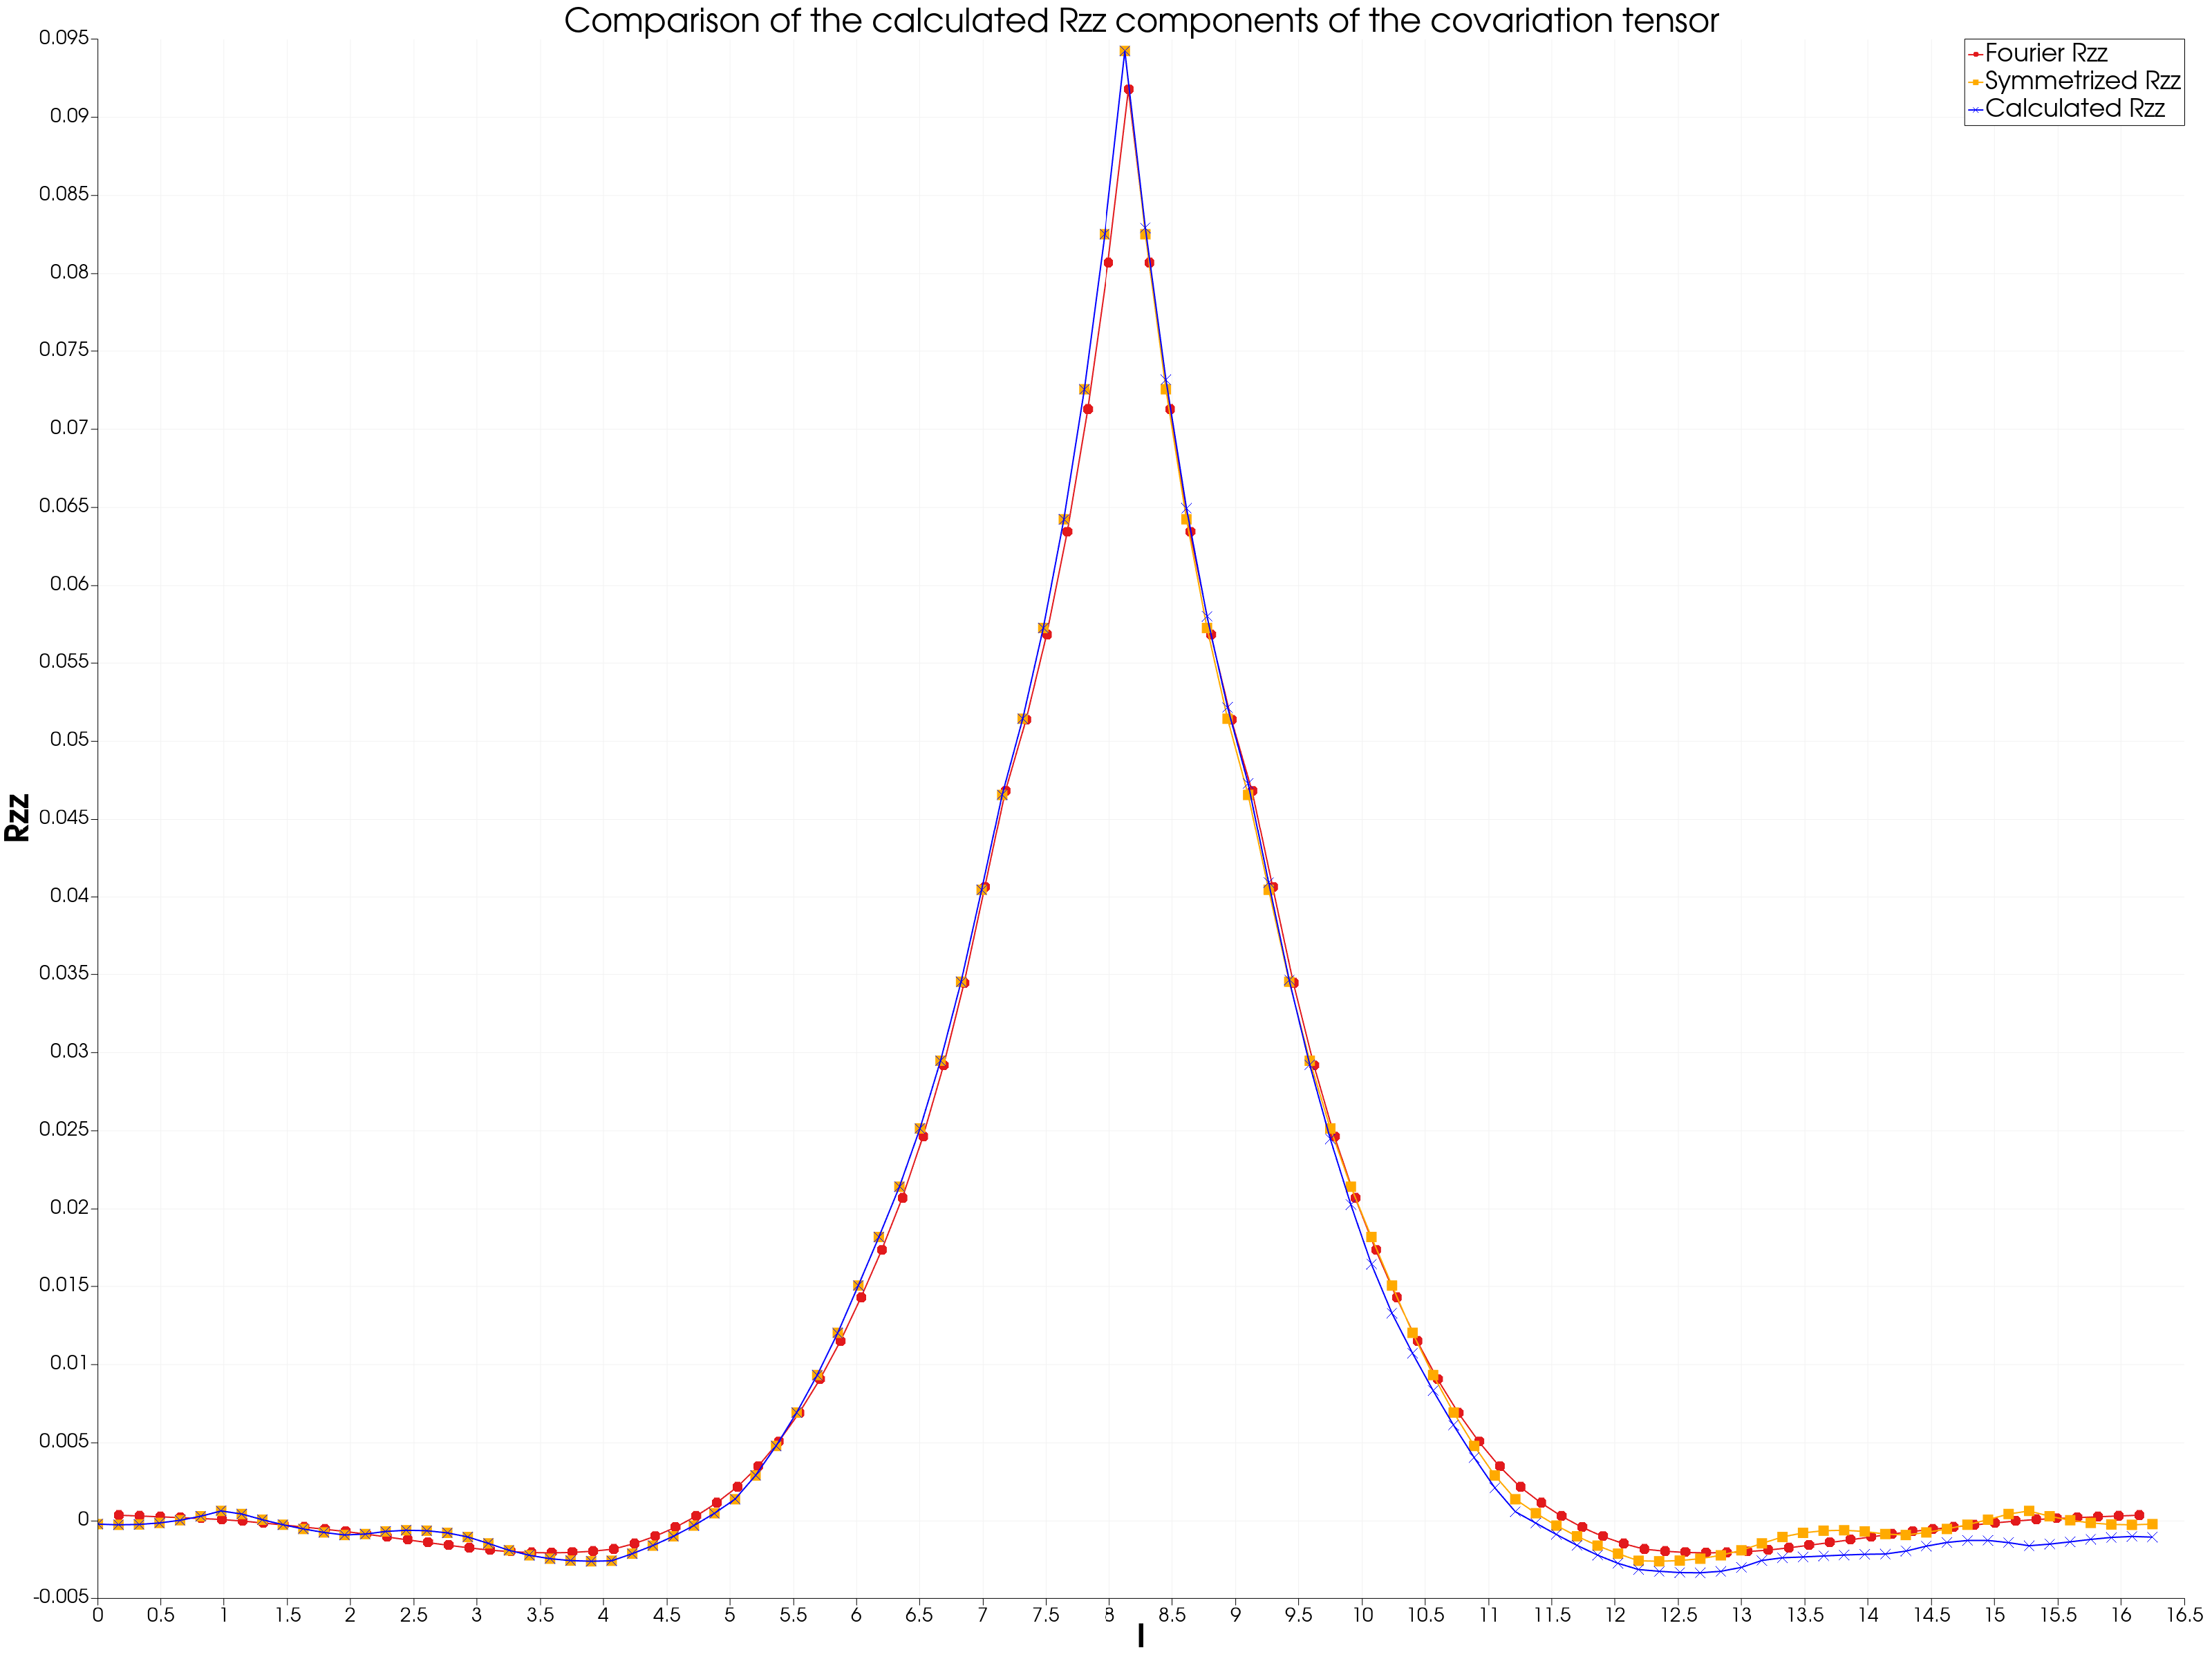
\includegraphics [width=0.8\linewidth] {images/kriging/3components/diagonal_r33_zz.png}
  \caption{Расчётная ковариационная функция $R_{zz}$ на основе стохастического метода вдоль диагонали области } 
  \label{img:kriging_covariances_diag}  
\end{figure}

По правой части графиков можно заметить насколько расчётная ковариационная функция не симметрична. Из-за этого дальнейшие расчёты тензора спектра скоростей и энергетического спектра проводились на симметризованной ковариационной функции. Процедура симметризации спектра необходима для устранения фазового смещения будущего тензора спектра скоростей, так как в ином случае при проведении преобразования Фурье, возникает мнимая часть, связанная с фазовым сдвигом, возникающим в следствии несимметричности функции, так как использовалось быстрое преобразование Фурье, требующее искусственного продолжения периодического сигнала. Возникающий скачок между продолженными ковариационными функциями, вносит фазовое смещение, откуда и возникает мнимая часть преобразования. Можно сказать, что мы рассматриваем не весь куб, а лишь его первый октант, данные для которого были симметрично продолжены относительно начала координат и граничащих плоскостей координат. 

Из-за мало корреляции компонент скоростей на больших расстояниях, также присутствуют большие отклонения ковариационной функции относительно задаваемой, что также вносит свою небольшую ошибку. Этот эффект отражается на последующем преобразовании Фурье при переходе от функций пространственной ковариации к тензору спектра скоростей. Ниже представлено сравнение расчётных значений тензора спектра скоростей с полученными применением формулы \eqref{eq:part3_2}. 
\noindent
\begin{figure}[!h]
    \center{
        \hfill
        \subcaptionbox[List-of-Figures entry]{$R_{xx}$\label{img:kriging_computed_phi_11_diagonal}} 
        {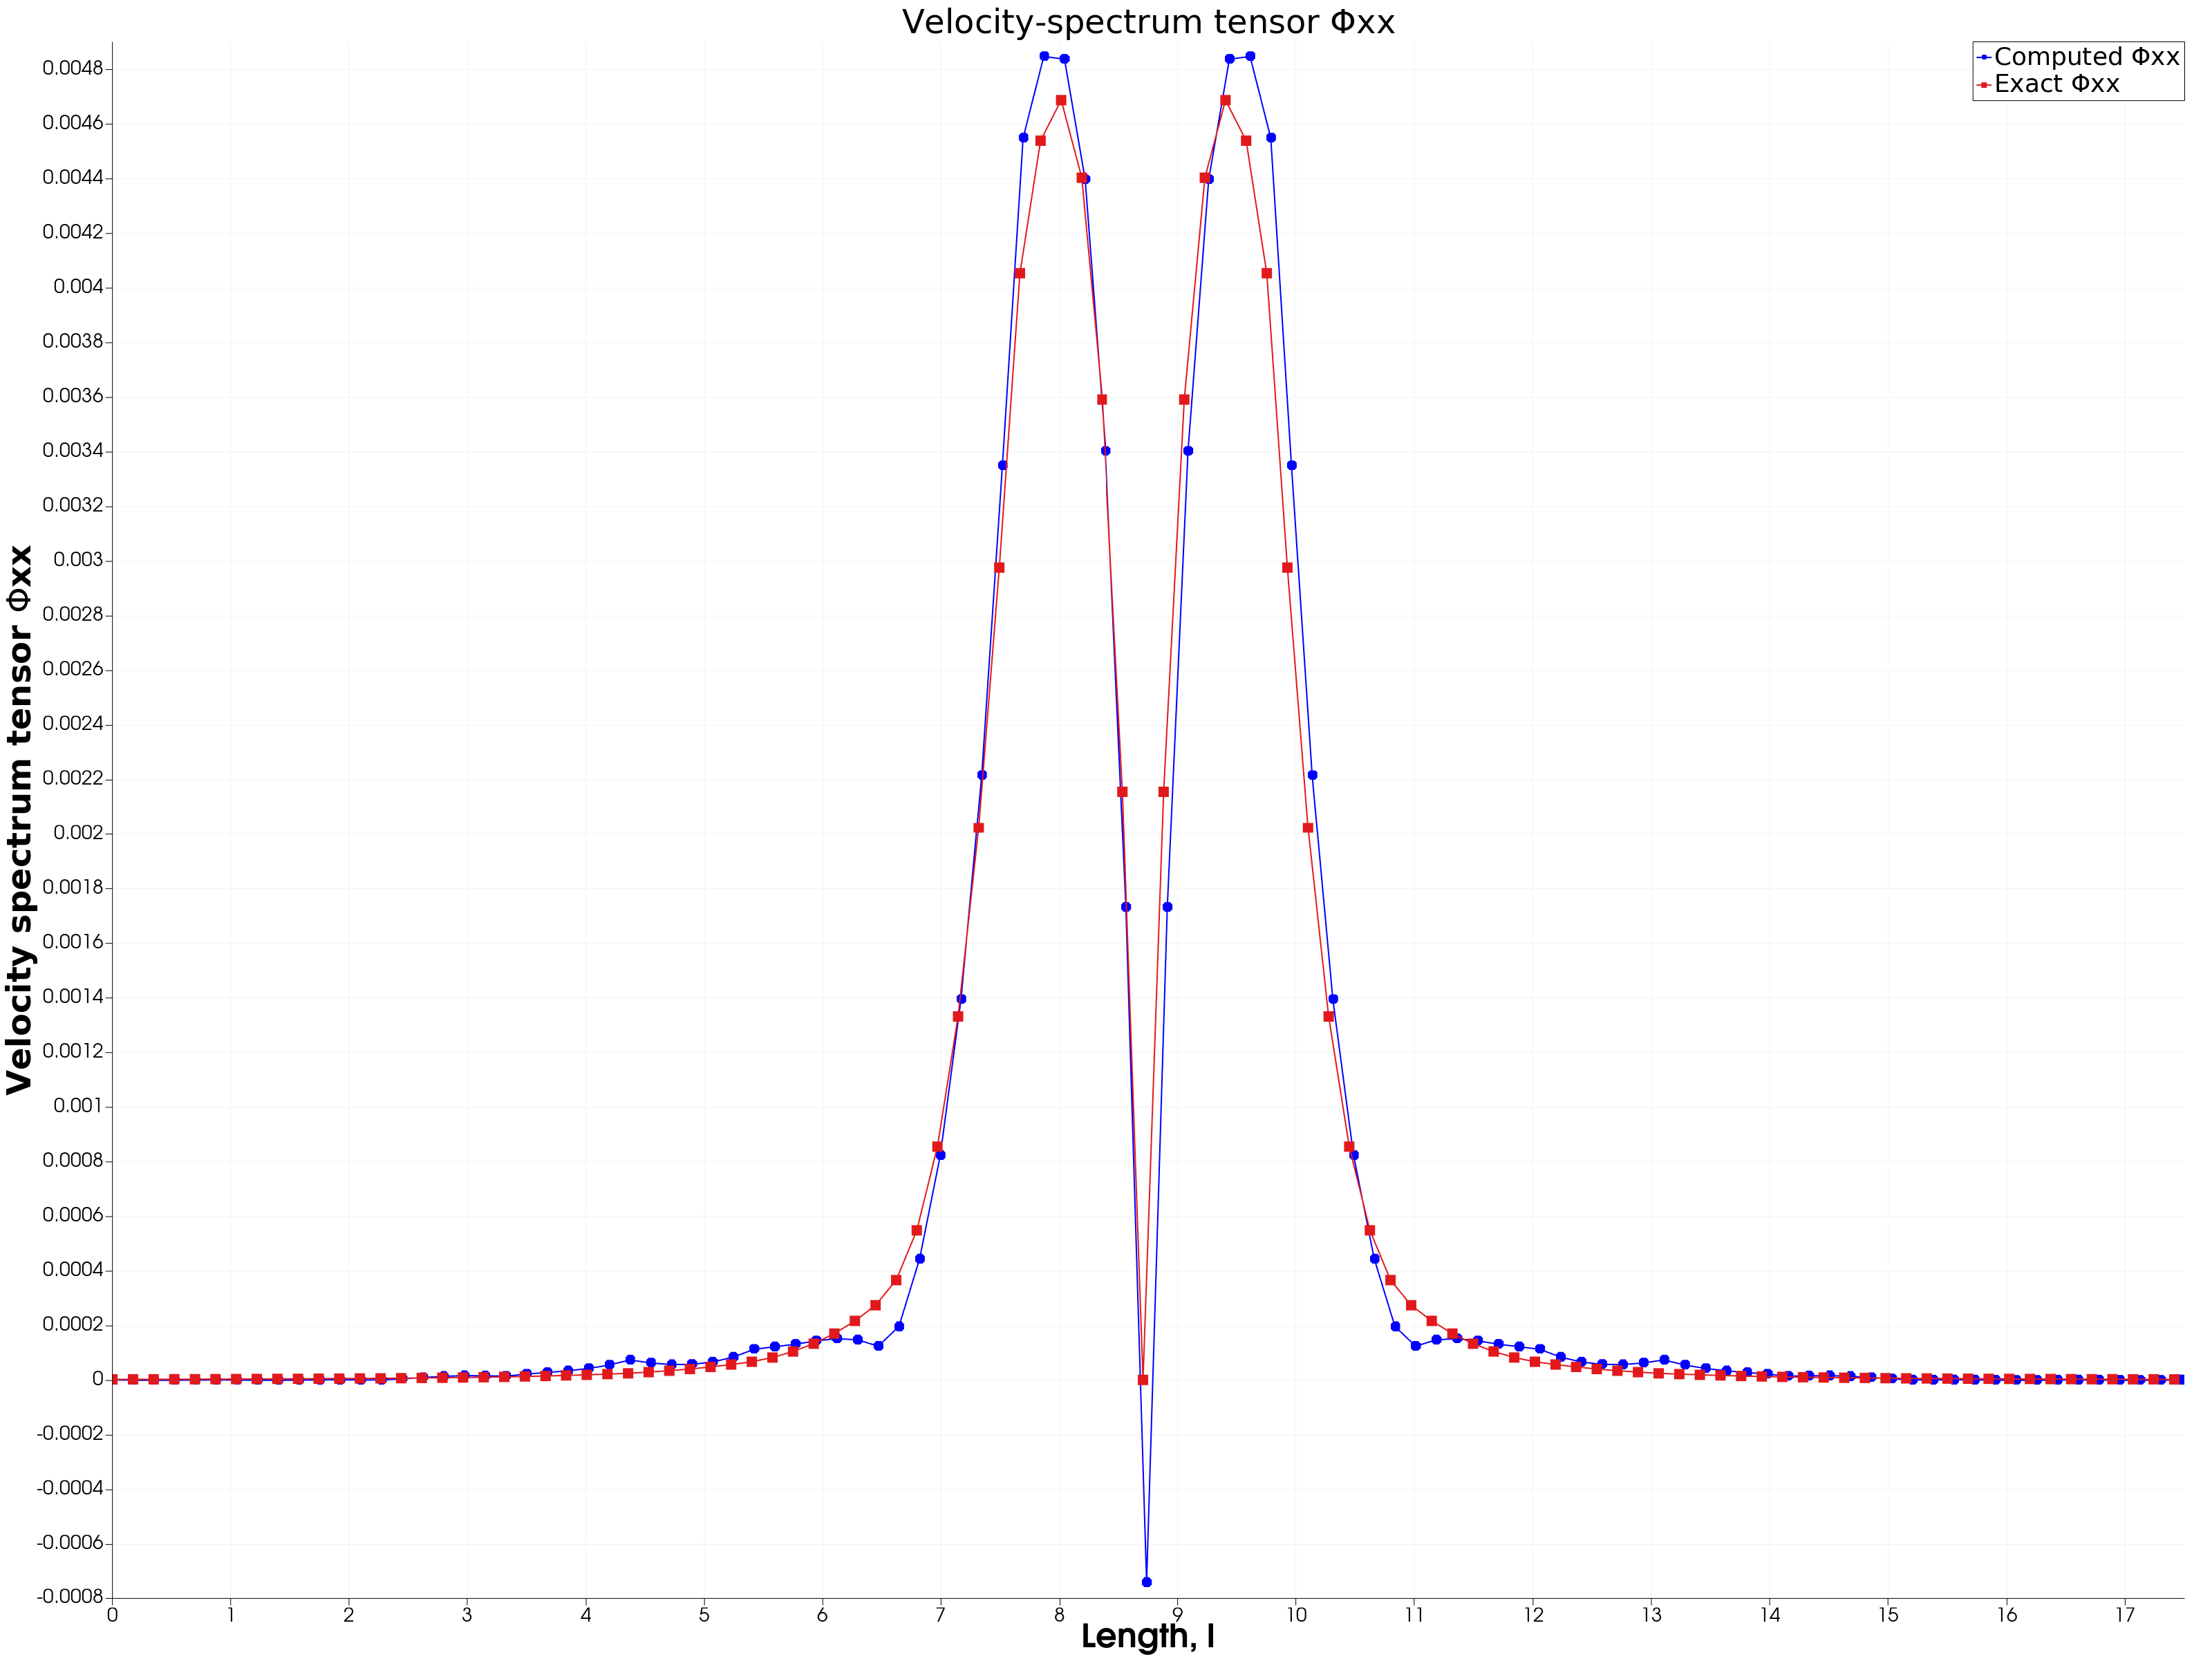
\includegraphics[width=0.34\linewidth]{images/kriging/3components/phi_11_diagonal.png}}%
        \hfill       
        \subcaptionbox{$R_{xy}$ и $R_{yx}$\label{img:kriging_computed_phi_12_diagonal}} 
        {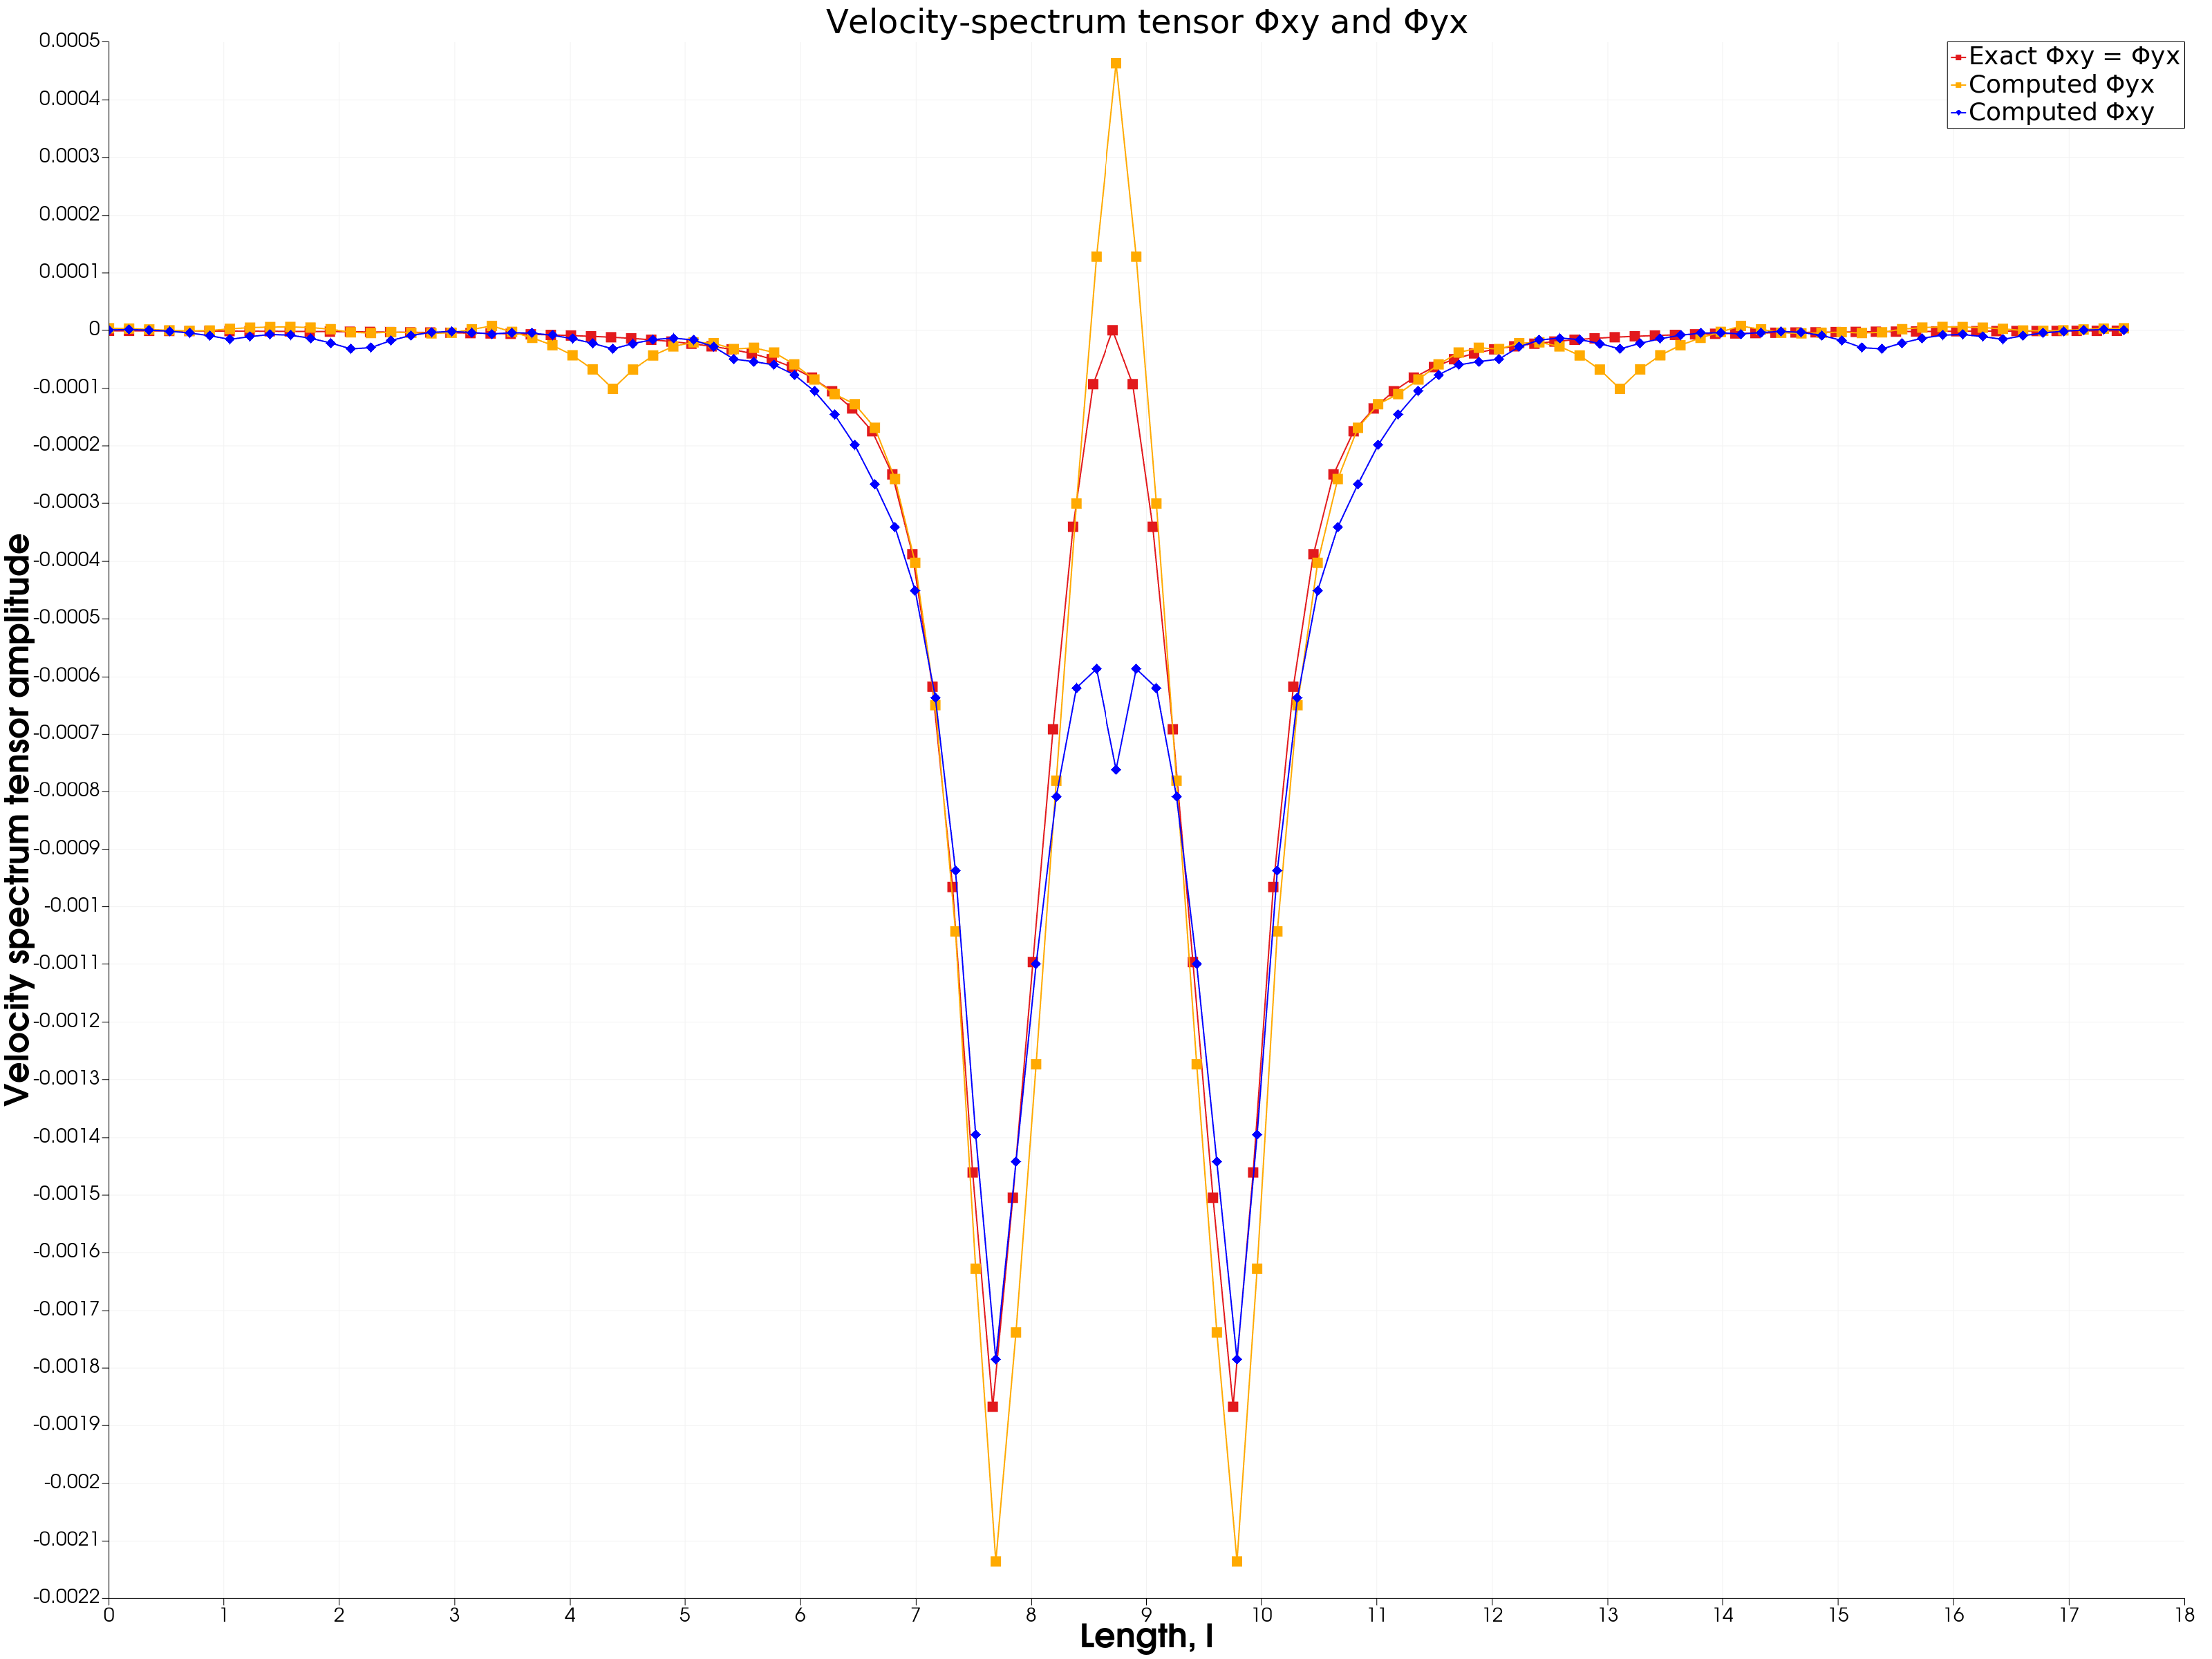
\includegraphics[width=0.34\linewidth]{images/kriging/3components/phi_12_21_diagonal.png}} \\
        \hfill
        \subcaptionbox{$R_{xz}$ и $R_{zx}$\label{img:kriging_computed_phi_13_diagonal}} 
        {\includegraphics[width=0.34\linewidth]{images/kriging/3components/phi_13_31_diagonal.png}}
        \hfill       
        \subcaptionbox{$R_{yy}$\label{img:kriging_computed_phi_22_diagonal}} 
        {\includegraphics[width=0.34\linewidth]{images/kriging/3components/phi_22_diagonal.png}} \\
        \hfill
        \subcaptionbox{$R_{yz}$ и $R_{yz}$\label{img:kriging_computed_phi_23_diagonal}} 
        {\includegraphics[width=0.34\linewidth]{images/kriging/3components/phi_23_32_diagonal.png}}
        \hfill
        \subcaptionbox{$R_{zz}$\label{img:kriging_computed_phi_33_diagonal}} 
        {\includegraphics[width=0.34\linewidth]{images/kriging/3components/phi_33_diagonal.png}}
        \hfill
    }
    
    \onehalfspacing{Функции тензора спектра энергий представлены дволь диагонали куба в пространстве фурье $n=17$, $k_l=10$}
    \caption{Ковариационные функции, заданные для применения трёхмерного стохастического метода}
    \label{img:exact_covariance_comparison_heat_maps}  
\end{figure}

Как можно заметить, основные различия между вычисленными и заданными компонентами тензора присутствуют при $\Phi \approx 0$. Далее используя формулу \eqref{eq:part3_2} перейдём от тензора спектра скоростей к энергетическому спектру. 

\begin{figure}[ht] 
  \center
  \includegraphics [width=0.9\linewidth] {images/kriging/3components/energy_function_kriging_loglog.png}
  \caption{Энергетический спектр поля скоростей полученный в результате стохастического моделирования в сравнении с целевым спектром в логарифмических координатах} 
  \label{img:kriging_spectra_function_compare}  
\end{figure}

Полученный спектр хорошо сходится с целевым спектров области наиболее энергонесущих мод. Есть сходство со спектром получаемым в результате метода Крайшнана, в частности резкое убывание, предположительно связанное с критерием Нейквиста.

Рассмотрим генерацию поля флуктуаций с использованием последовательного моделирования. Как говорилось в \ref{chapt1}, в данном случае, основным параметров генерации, который мы можем варьировать -- число ближайших соседей, учитываемых при расчёта среднего и ковариации величины в точке. Наиболее оптимальным оказалось число $N=15$ при котором наблюдается хорошая аппроксимация целевого спектра, а также достаточно высокая производительность. Для обычного непоследовательного стохастического метода, помимо высокого затрачиваемого процессорного времени, требуется достаточно большой объём памяти, что может сильно ограничить возможность генерации на подробных сетках. В свою очередь, метод последованных симуляций позволяет сократить требуемое количество памяти, за счёт отказа от хранения матрицы ковариаций целиком (теперь необходимо хранить матрицы $n \times n$). Малое число параметров, позволяет более простым образом задать требуемый спектр. Ниже представлено сравнение спектров, результирующего, полученного с использованием 1000 реализаций поля генерируемого последовательным методом. Параметры сеток задавилсь следующими: для сетки пространства Фурье $l_F=20$, $n_F = 51$, для сетки физического пространства $n_{P} = 31$, $l=10$. Число учитываемых ближайших соседей $N = 15$.

\begin{figure}[ht] 
    \center
    \includegraphics [width=0.8\linewidth] {images/kriging/spectrum.png}
    \caption{Сравнение энергетического спектра для предлагаемой модиификации спектрального метода с целевым} 
    \label{img:kriging_result_field_no_angle}  
\end{figure}

\begin{figure}[ht] 
    \center
    \includegraphics [width=0.8\linewidth] {images/kriging/spectrum_loglog.png}
    \caption{Сравнение энергетического спектра для предлагаемой модиификации спектрального метода с целевым в логарифмических координатах} 
    \label{img:kriging_result_field_on_angle}  
\end{figure}

Как и в случае спектрального метода, наблюдается разница в спектрах для малых волновых чисел, в остальном, особенно в инерционном интервале, получаем практически точное сходство. Наибольшое отклонение результирующего от задаваемого спектров $\Delta E = 0.025$, но также стоит отметить, что это значение находится в волнвых числах меньше чем минимальное волнове число на сетке $k_{min}=\frac{2 \pi}{10} \approx 0.628$. Как было сказано выше основным критерием выбора метода является удовлетворению целевому спектру. Рассмотрим сравнение полученных спектров обоими методами с целевым спектром.

\begin{figure}[ht] 
    \center
    \includegraphics [width=0.8\linewidth] {images/comparison_of_result_spectras.png}
    \caption{Сравнение энергетического спектра для предлагаемой модиификации спектрального метода с целевым в логарифмических координатах} 
    \label{img:main_comparison_of_target_spectras}  
\end{figure}

Для полей получаемых по результатам спектрального метода, наблюдается лучшая точность при малых волновых числах, с учётом того что существуют ограничения на волновые числа многократно описанные выше. Метод последовательных симуляций лучшим образом аппроксиммирует спектр в инерционном интервале, а также имеет более точное совпадение пика для наиболее энергонесущей волны. Но по сравнению со спектральным методом, данный имеет большее затрачиваемое время на одну реализацию. С сетки и параметра $N$ описанных выше, генерация 1000 полей происходит за 2 минуты 14 секунд, одна реализация требует $\frac{134}{1000} \approx 0.134$ секунд, без учёта времени на запись результатов, результат больше чем требуется для спектрального метода в 3 раза.